% !TEX root = FDS_Validation_Guide.tex

\chapter{Description of Experiments}

\label{Experiments_Chapter}

This chapter contains a brief description of the experiments that were used for model validation. Only enough detail is included here to provide a general understanding of the model simulations. Anyone wishing to use the experimental measurements for validation ought to consult the cited test reports or other publications for a comprehensive description.


\section{ArupFire Tunnel Fire Experiments}
\label{ArupFire_Tunnel_Fire_Description}

Gabriele Vigne and Jimmy J\"{o}nsson of ArupFire conducted a series of fire experiments within a tunnel with a 50~m$^2$ cross section. The tunnel is located in La Ribera del Folgoso, Spain. It is approximately 6.5~m high, 8~m wide and 300~m long. Five replicate tests were conducted using a 1~m by 2~m steel pan filled with heptane on water. Near-ceiling temperatures were measured 2~m, 4~m, 6~m and 8~m from the plume centerline. The peak heat release rate was approximately 5.3~MW.


\section{ATF Corridors Experiments}
\label{ATF_Corridors_Description}

A series of eighteen experiments were conducted in a two-story structure with long hallways and a connecting stairway in the large burn room of the ATF Fire Research Laboratory in Ammendale, Maryland, in 2008~\cite{Sheppard:Corridors}. The test enclosure consisted of two 17.0~m long hallways connected by a stairway consisting of two staircases and an intermediary landing. There was a door at the opposite end of the first floor hallway, which was closed during all tests. The end of the second floor hallway was open with a soffit near the ceiling.

The walls and ceilings of the test structure were constructed of 1.2~cm gypsum wallboard. The flooring throughout the structure, including the stairwell landing floor, consisted of one layer of 1.3~cm thick cement board on one layer of 1.9~cm thick plywood supported by wood joists. The first set of stairs, which had eight risers, led from the first floor up to the landing area. The second set of stairs, which had nine risers, led from the landing area up to the second floor. The stairs were constructed of 2.5~cm thick clear pine lumber. The two set of stairs were separated by an approximately 0.42~m wide gap in the middle of the stairwell. This gap was separated from the stairs by a 0.91~m tall barrier constructed of a single piece of gypsum board. The flue space was open to the first floor.  The flue space was separated from the second floor by a 0.9~m tall barrier constructed of gypsum board. There was a metal exterior type door at the end of the first floor near the burner.  The door was closed during all experiments.

The fire source was a natural gas diffusion burner.  The burner surface was horizontal, square and 0.45~m on each side, its surface was 0.37~m above the floor, and it was filled with gravel. The burner was located near the end of the first floor away from the stairs. A diagram of the test structure is displayed in Figure~\ref{ATF Drawing}.

\begin{figure}[p]
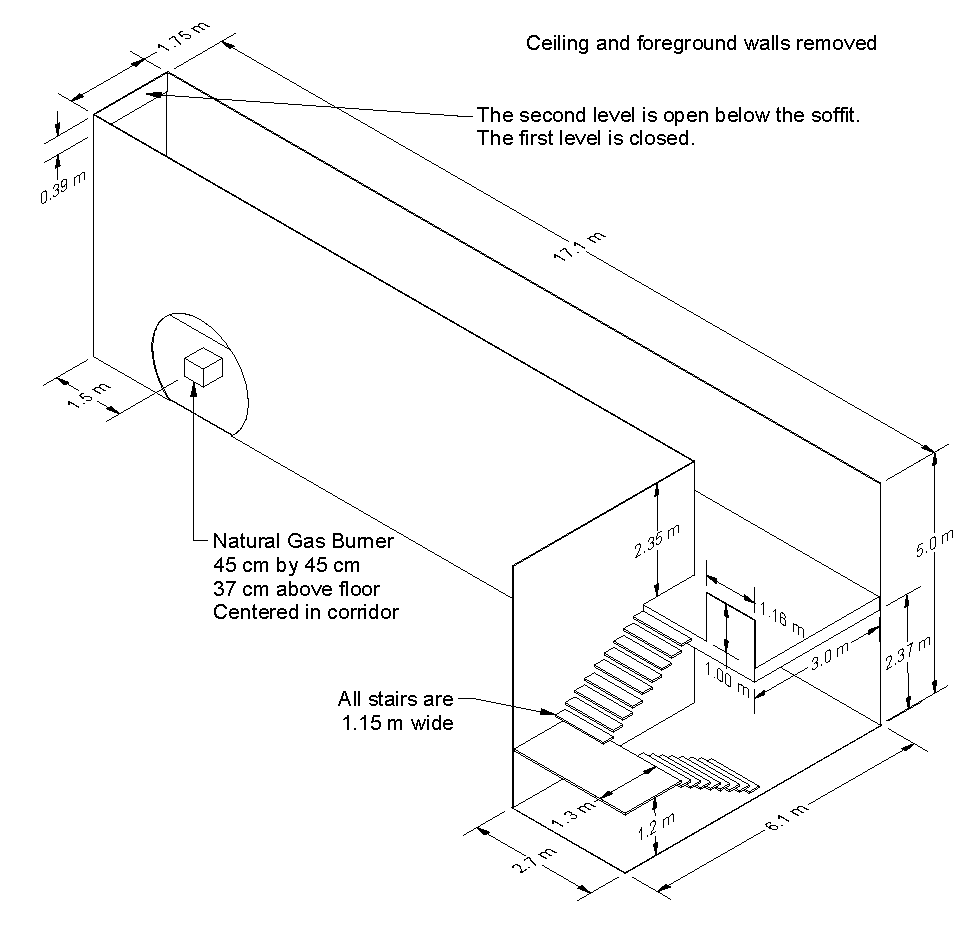
\includegraphics[width=\textwidth]{FIGURES/ATF_Corridors/ATF_Corridors_Drawing}
\caption{Geometry of the ATF Corridors Experiments.}
\label{ATF Drawing}
\end{figure}


\section{Atmospheric Dispersion Correlations}
\label{Atmospheric_Dispersion_Description}

A common exercise in atmospheric dispersion modeling is predicting the plume rise height of stack emissions. Stull~\cite{Stull:2000} presents an empirical correlation for plume rise height from a smoke stack in a stable atmospheric boundary layer. Details of the correlation and simulation are found in Section~\ref{Plume_Height_Discussion}.



\section{Backward Facing Step}
\label{Backward_Facing_Step_Description}

A common validation experiment for CFD codes involves flow through a channel with a backward facing step. These experiments are designed to test the influence of grid resolution, inlet turbulence, wall boundary treatments, and eddy viscosity models. One set of experiments has been conducted by Jovic and Driver~\cite{JD:1994}.  A schematic view of the experiment is shown in Fig.~\ref{tunnel_drawing}. The dimensions of the channel are based on step height $h$ = 0.0098 m.  The length of the channel is $24 \, h$. The width of the channel is $4 \, h$. The height of the inlet section is $5 \, h$, and the height of the channel downstream of the step is $6 \, h$. The expansion ratio is thus 1.2.  The inlet is split into three sub-inlets to permit localized variation of inlet turbulence.  The Reynolds number of the flow is 5100, based on the free-stream velocity (7.2~m/s) and the step height.

\begin{figure}[!ht]
\includegraphics[width=\textwidth]{FIGURES/Backward_Facing_Step/tunnel_drawing}
\caption[Geometry of the Backward Facing Step experiments]{Geometry of the Backward Facing Step experiments.}
\label{tunnel_drawing}
\end{figure}


\section{Beyler Hood Experiments}
\label{Beyler_Hood_Description}

Craig Beyler performed small-scale fire experiments where a variety of circular gas burners were centered at various heights underneath a closed, cylindrical hood, 100~cm in diameter and 48~cm in height~\cite{Beyler:Hood}.  The hood consisted of two concentric cylinders separated by an air gap, as shown in Fig.~\ref{Beyler_Hood_Sketch}.  The inner cylinder was shorter than the outer and this allowed combustion products to be removed uniformly from the hood perimeter.  The exhaust gases were then analyzed to determine species concentrations. The burner could be raised and lowered with respect to the bottom edge of the hood. The reported relative standard uncertainty of the measured gas species mass fractions was 6~\%. The fuels consisted of acetone, ethanol, isopropanol, methanol, propane, propylene, and toluene. Hood equivalence ratios varied from 0.2 to 1.7.  A subset of 47 of the original 148 experiments spanning the equivalence ratio range for each fuel were simulated for validation, see Table~\ref{beyler_sum}.

\begin{figure}[h]
\centering
\includegraphics[width=\textwidth]{FIGURES/Beyler_Hood/Beyler_Hood}
\caption[Sketch of Beyler Hood cross section]{Sketch of Beyler Hood cross section.}
\label{Beyler_Hood_Sketch}
\end{figure}

\begin{table}[!ht]
\centering
\caption[Summary of simulated Beyler Hood experiments]{Summary of simulated Beyler Hood experiments. A negative value of Separation Distance indicates the burner top is below the lower rim of the hood.}
\label{beyler_sum}
\begin{tabular}{|c|c|c|c|c||c|c|c|c|c|}
\hline
Exp.   & Fuel          & HRR      & Burner           & Sep.           &  Exp.   & Fuel          & HRR      & Burner           & Sep.            \\
No.    & Gas           & (kW)     & (cm)             & Dist. (cm)     &  No.    & Gas           & (kW)     & (cm)             & Dist. (cm)      \\ \hline \hline
117    & Acetone       & 18.0     & 22.6             & -12            &  232    & Propane       & 13.5     & 19.5             & -5              \\ \hline
119    & Acetone       & 16.4     & 22.6             & -1             &  257    & Propane       & 8.2      & 19.5             & -15             \\ \hline
122    & Acetone       & 16.4     & 22.6             & 4              &  287    & Propane       & 7.9      & 19.5             & 5               \\ \hline
142    & Acetone       & 12.1     & 22.6             & 4              &  303    & Propane       & 18.3     & 19.5             & 5               \\ \hline
145    & Acetone       & 12.7     & 22.6             & 4              &  307    & Propane       & 21.4     & 19.5             & 5               \\ \hline
106    & Ethanol       & 17.3     & 22.6             & -9             &  318    & Propane       & 18.3     & 19.5             & -20             \\ \hline
107    & Ethanol       & 21.3     & 22.6             & -4             &  322    & Propane       & 21.4     & 19.5             & -20             \\ \hline
108    & Ethanol       & 17.3     & 22.6             & 4              &  334    & Propane       & 21.4     & 19.5             & -15             \\ \hline
110    & Ethanol       & 13.5     & 22.6             & 4              &  355    & Propane       & 18.3     & 19.5             & 0               \\ \hline
115    & Ethanol       & 13.5     & 22.6             & 4              &  359    & Propane       & 21.4     & 19.5             & 0               \\ \hline
130    & Isopropanol   & 12.4     & 22.6             & 4              &  371    & Propane       & 21.4     & 19.5             & -5              \\ \hline
132    & Isopropanol   & 12.4     & 22.6             & 4              &  389    & Propane       & 18.3     & 19.5             & 0               \\ \hline
133    & Isopropanol   & 12.4     & 22.6             & 4              &  429    & Propane       & 28.1     & 19.5             & -10             \\ \hline
136    & Isopropanol   & 12.4     & 22.6             & -1             &  433    & Propane       & 31.5     & 19.5             & -10             \\ \hline
141    & Isopropanol   & 12.4     & 22.6             & 4              &  445    & Propane       & 31.5     & 19.5             & -15             \\ \hline
942    & Methanol      & 11.0     & 22.6             & 0              &  780    & Propylene     & 7.5      & 19.5             & -10             \\ \hline
943    & Methanol      & 11.0     & 22.6             & 0              &  805    & Propylene     & 7.5      & 19.5             & -10             \\ \hline
945    & Methanol      & 11.0     & 22.6             & -5             &  859    & Propylene     & 31.4     & 19.5             & -10             \\ \hline
947    & Methanol      & 11.0     & 22.6             & 0              &  870    & Propylene     & 19.0     & 19.5             & -2              \\ \hline
951    & Methanol      & 9.8      & 22.6             & 0              &  882    & Propylene     & 19.1     & 19.5             & -10             \\ \hline
160    & Toluene       & 11.5     & 22.6             & -6             &  886    & Propylene     & 19.1     & 19.5             & -5              \\ \hline
162    & Toluene       & 11.5     & 22.6             & -1             &  910    & Propylene     & 31.4     & 19.5             & -11             \\ \hline
165    & Toluene       & 11.5     & 22.6             & 4              &  \multicolumn{5}{c|}{}                                                  \\ \cline{1-5}
166    & Toluene       & 11.5     & 22.6             & 5              &  \multicolumn{5}{c|}{}                                                  \\ \cline{1-5}
170    & Toluene       & 11.5     & 22.6             & 4              &  \multicolumn{5}{c|}{}                                                  \\ \hline
\end{tabular}
\end{table}

\subsubsection{Modeling Notes}

Simulations of the Beyler Hood experiments are performed at 3~cm resolution within a fairly simple facsimile of the actual hood. The boundary conditions are set to adiabatic to allow for a relatively quick ramp up to steady-state conditions.

The two-step simple chemistry combustion scheme is applied, where an infinitely fast reaction converts the fuel to CO, soot, and water vapor, followed sequentially by a second fast reaction that converts the soot and CO to CO$_2$. Some of the soot and CO does not convert to CO$_2$, based on post-flame yields listed by Tewarson~\cite{SFPE:Tewarson}.

A minimum auto-ignition temperature is specified for each fuel~\cite{SFPE:Beyler} to prevent the fuel vapor from igniting at the layer interface. This restriction is relaxed in the grid cells just above the burner surface to allow for ignition without a secondary heat source. In addition, a critical flame temperature of 500~$^\circ$C is applied in all cases to account for local flame extinction. The grid is too coarse to support the actual values, and the chosen value is a placeholder until a better flame extinction model is developed.

\section{BGC/GRI LNG Fire Experiments}
\label{BGC_GRI_LNG_Fires_Description}

In 1982 and 1983, P.A. Croce and K.S. Mudan of Arthur D. Little, Inc., and J. Moorhouse of the British Gas Corporation (BGC) supervised 13 liquified natural gas (LNG) trench fire experiments conducted by BGC on behalf of the Gas Research Institute (GRI)~\cite{Croce:GRI}. Thirteen experiments were performed with nominal trench sizes ranging from 0.8~m by 4.4~m to 3.9~m by 52~m and aspect ratios ranging from approximately 5 to 30. Wind speeds varied from approximately 1~m/s to almost 10~m/s. Measurements made during the tests included flame geometry, radiative heat flux, emissive power, burning rate, LNG liquid and vapor compositions, and meteorological data. The fires were observed to exhibit substantial flame drag and flame breakup, unlike low aspect ratio pools. Steady burning was achieved in all tests.

The key parameters for each experiment are listed in Table~\ref{BGC_sum}. The Flame Tilt angle is the measured deflection of the flame from the vertical. The Flame Drag Ratio is the distance that the flame drags along the ground outside of the trench added to the trench width, and then divided by the trench width. The Avg.~Flame Length denotes the time-averaged flame length, while the Max.~Flame Length refers to the time-averaged extent of the fluctuating flame tips.

\begin{table}[!ht]
\centering
\caption[BGC/GRI LNG Fires test parameters]{BGC/GRI LNG Fires test parameters.}
\label{BGC_sum}
\begin{tabular}{|c|c|c|c|c|c|c|c|c|c|}
\hline
Test  & Trench     & Trench    & Aspect  & Wind        & Burning           & Flame       & Flame       & Avg.~Flame  & Max.~Flame  \\
No.   & Length     & Width     & Ratio   & Speed       & Rate              & Tilt        & Drag        & Length      & Length      \\ 
      &        (m) &       (m) &         & (m/s)       & (kg/m$^2$/s)      & (deg)       & Ratio       &        (m)  &        (m)  \\ \hline
1     & 23.53      & 1.81      & 13.00   & 3.8         & 0.064             & 56.3        & 2.57        & 4.4         & 8.9         \\ \hline
2     & 15.52      & 1.81      & 8.57    & 1.5         & 0.069             & 56.1        & 2.30        & 3.8         & 7.3         \\ \hline
3     & 9.23       & 1.83      & 5.04    & 1.0         & 0.098             & 45.2        & 1.21        & 7.1         & 11.4        \\ \hline
4     & 23.50      & 1.83      & 12.84   & 8.36        & 0.054             & 56.8        & 2.96        & 3.4         & 7.3         \\ \hline
5     & 9.05       & 1.82      & 4.97    & 9.31        & 0.060             & 60.5        & 2.96        & 4.2         & 8.2         \\ \hline
6     & 23.45      & 3.94      & 5.95    & 4.98        & 0.082             & 59.6        & 2.62        & 6.9         & 16.8        \\ \hline
7     & 23.45      & 0.82      & 28.60   & 3.80        & 0.049             & 48.3        & 3.98        & 2.0         & 4.3         \\ \hline
8     & 11.82      & 0.82      & 14.41   & 2.05        & 0.058             & 49.8        & 3.77        & 2.1         & 4.6         \\ \hline
9     & 9.10       & 0.82      & 11.10   & 5.40        & 0.051             & 47.0        & 3.68        & 1.5         & 3.7         \\ \hline
10    & 52.05      & 3.89      & l3.38   & 7.05        & 0.060             & 61.3        & 2.83        & 7.9         & 20.3        \\ \hline
11    & 4.37       & 0.81      & 5.40    & 5.90        & 0.052             & 49.9        & 4.16        & 1.8         & 3.6         \\ \hline
12    & 52.15      & 1.82      & 28.65   & 8.60        & 0.046             & 61.3        & 3.70        & 3.3         & 8.1         \\ \hline
13    & 23.10      & 0.77      & 30.00   & 3.69        & 0.043             & 55.7        & 4.23        & 2.1         & 5.3         \\ \hline
\end{tabular}
\end{table}

\subsubsection{Modeling Notes}

The experiments are simulated using the specified fuel burning rate. The fuel is assumed to be methane. The atmosphere is assumed to be neutral with a large Obukhov length, $L=1000000$, and the ground surface is flat with an assumed aerodynamic roughness, $z_0=0.1$~m. The relative humidity, ambient temperature and pressure, and wind speed at 9~m are specified in the report. The radiative fraction is assumed to 0.25 and the radiative path length is assumed to be 50~m; that is, the effective absorption coefficients of the various gas mixtures are evaluated over a distance of 50~m. The radiation source term is taken directly as 25~\% of the combustion energy release rate. The soot yield is assumed to be 0.005.

\begin{description}
\item[Flame Height Results:] Section~\ref{Flame Height} 
\item[Flame Tilt Results:] Section~\ref{Flame Tilt} 
\item[Heat Flux Results:] Section~\ref{BGC_GRI_LNG_Fires_Heat_Flux} 
\end{description}

\FloatBarrier


\section{Bittern Sprinkler Experiments}
\label{Bittern_Sprinkler_Description}

In 2004, a set of 22 fire experiments was conducted at the University of Canterbury, New Zealand, by Adam Bittern~\cite{Bittern:Thesis,Wade:FT2007}. In each experiment, a single chair was burned within an enclosure with two sprinklers installed. The sprinklers were not charged with flowing water during the experiments, but pressure gauges were installed immediately upstream of each sprinkler to indicate activation. The sprinkler actuation time, chair mass loss rate, and gas temperature profile were measured. The HRR was estimated from the measured mass loss rate and heat of combustion of the fuel.

The experiments incorporated four different types of sprinklers, two fire locations (the center and corner of the enclosure), and two ventilation conditions (open or closed door). The enclosure was timber-framed and lined with 10~mm thick gypsum plasterboard. The door was made of plywood and was 0.8~m wide by 2.1~high. The compartment layout, dimensions and experimental arrangement are shown in Figure~\ref{bit_plan}. The chair used as fuel for each experiment was made of flexible polyurethane foam slabs, where each slab measured approximately 0.5~m by 0.4~m by 0.1~m. The seat was ignited using a solid petroleum lighter.

Table~\ref{bit_sum} reports the sprinkler actuation times of each sprinkler.

\begin{figure}[h]
\centering
\includegraphics[width=\textwidth]{FIGURES/Bittern_Sprinkler_Experiments/Bittern_Sketch}
\caption[Plan view of the Bittern Sprinkler Experiments]{Plan view of the Bittern Sprinkler Experiments.}
\label{bit_plan}
\end{figure}


\begin{table}[!ht]
\centering
\caption[Summary of results, Bittern experiments]{Summary of results, Bittern experiments. Note that Exp.~11 has been excluded because of a failed mass loss measurement.}
\label{bit_sum}
\begin{tabular}{|c|c|c|c|c|c|c|c|}
\hline
Exp. & Spr.~1 & Time (s) & Spr.~2 & Time (s) & $T_0$ ($^\circ$C) & Door   & Fire Position \\ \hline \hline
1    & Res A  & 210      & Res A  & 250      & 23.7              & Open   & Center        \\ \hline
2    & Res A  & 225      & Res A  & 211      & 25.5              & Open   & Center        \\ \hline
3    & Res B  & 192      & Res B  & 192      & 25.5              & Open   & Center        \\ \hline
4    & SS68   & 226      & SS68   & 226      & 25.7              & Open   & Center        \\ \hline
5    & SS68   & 266      & SS68   & 272      & 27.5              & Open   & Center        \\ \hline
6    & SS68   & 216      & SS68   & 211      & 27.7              & Open   & Center        \\ \hline
7    & Res A  & 182      & Res A  & 186      & 28.2              & Open   & Center        \\ \hline
8    & Res B  & 182      & Res B  & 187      & 27.9              & Open   & Center        \\ \hline
9    & Res B  & 233      & Res B  & 230      & 28.9              & Open   & Center        \\ \hline
10   & Res A  & 183      & Res B  & 184      & 29.4              & Open   & Center        \\ \hline
12   & SS68   & 246      & Res B  & 228      & 24.0              & Closed & Center        \\ \hline
13   & SS68   & 204      & Res B  & 194      & 24.5              & Closed & Center        \\ \hline
14   & SS68   & 203      & Res B  & 187      & 24.2              & Closed & Center        \\ \hline
15   & SS68   & 270      & Res B  & 253      & 23.7              & Closed & Center        \\ \hline
16   & Res B  & 178      & Res A  & 224      & 20.6              & Closed & Corner        \\ \hline
17   & Res B  & 181      & Res A  & 228      & 23.8              & Closed & Corner        \\ \hline
18   & SS68   & 187      & Res A  & 221      & 25.0              & Closed & Corner        \\ \hline
19   & SS68   & 189      & Res A  & 223      & 26.4              & Closed & Corner        \\ \hline
20   & SS68   & 205      & Res A  & DNA      & 25.3              & Closed & Corner        \\ \hline
21   & SS93   & 216      & SS93   & 330      & 25.2              & Closed & Corner        \\ \hline
22   & SS93   & 205      & SS93   & 263      & 25.2              & Closed & Corner        \\ \hline
\end{tabular}
\end{table}

\subsubsection{Modeling Notes}

The assumptions given in this section were used in the original analysis of the experiments~\cite{Bittern:Thesis}.

The gypsum board had a thickness of 1~cm, density of 731~kg/m\textsuperscript{3}, specific heat of 0.90~kJ/(kg$\cdot$K), conductivity of 0.17~W/(m$\cdot$K), and emissivity of 0.88. The concrete floor was assumed to have a thickness of 10~cm, density of 2300~kg/m$^3$, specific heat of 0.88~kJ/(kg$\cdot$K), conductivity of 1.2~W/(m$\cdot$K), and emissivity of 0.5.

The properties of the sprinklers are shown in Table~\ref{Bittern_Sprinklers}. These properties are based on the manufacturer's specification where available or otherwise estimated based on measured values of comparable sprinklers. For modeling purposes, the sprinkler offset, 2~cm, was selected based on an approximate 2~cm glass bulb length, and the C-factor selected was based on a sensitivity analyses undertaken in the original study.

\begin{table}[!ht]
\centering
\caption[Properties of sprinklers used in Bittern Experiments]{Properties of sprinklers used in Bittern Experiments.}
\label{Bittern_Sprinklers}
\begin{tabular}{|l|l|c|c|c|}
\hline
\textbf{Short} & \textbf{Description}                & \textbf{RTI}        & \textbf{C-Factor} & \textbf{Act. Temp.} \\
\textbf{Name}  &                                     & (m$\cdot$s)$^{1/2}$ & (m/s)$^{1/2}$     & $^\circ$C           \\ \hline
Res A          & Residential, 3 mm glass bulb        & 36                  & 0.4               & 68                  \\ \hline
Res B          & Residential, 3 mm glass bulb        & 36                  & 0.4               & 68                  \\ \hline
SS68           & Standard Response, 5 mm glass bulb  & 95                  & 0.4               & 68                  \\ \hline
SS93           & Standard Response, 5 mm glass bulb  & 95                  & 0.4               & 93                  \\ \hline
\end{tabular}
\end{table}

The average heat of combustion of the upholstery was measured in a cone calorimeter to be 21.9~MJ/kg (Exp.~1-10) and 20.4~MJ/kg (Exp.~12-22). Since the primary fuel used in the experiments was flexible polyurethane foam, the radiant loss fraction assumed in the fire model was 0.46. Other combustion parameters were as for polyurethane foam, and all parameters selected are consistent with those used in the original BRANZFIRE study~\cite{Wade:FT2007}. For the ``simple chemistry'' combustion model, inputs for stoichiometric yields have been selected from literature based on GM23 foam, with an effective molecular formula of CH$_{1.8}$O$_{0.35}$N$_{0.06}$. The soot yield was assumed to be 0.227~kg/kg. The area of the fire was taken to be 0.4~m by 0.5~m. The height of the fire was assumed to be 0.65~m above the floor.

For experiments 11 to 22, the door to the compartment was closed. The estimated leakage area was assumed based on data for loose-fitting internal walls. An area of 0.053 m\textsuperscript{2} was evenly distributed across the door.


\section{Bouchair Solar Chimney}
\label{Bouchair_Solar_Chimney_Description}

To evaluate solar-induced ventilation systems in desert climates, Bouchair~\cite{Bouchair:Thesis} constructed a simple test apparatus shown in Fig.~\ref{Bouchair_Drawing}. A compartment with interior dimensions of approximately 1.6~m long, 1.8~m, and 2.0~m high had a window on one side and an air inlet slot on the other, leading into a 1.5~m wide cavity with two heating panels spanning the long dimension. The panels were heated to 10~$^\circ$C, 20~$^\circ$C, 30~$^\circ$C, or 40~$^\circ$C above ambient, drawing air through the compartment and into the thermal cavity. The mass flow rate of air through the cavity was measured. The inlet slot was either 0.1~m or 0.4~m high, and 1.4~m wide. The thermal cavity was 1.5~m wide, and the hot panels were separated by 0.1~m, 0.2~m, 0.3~m, 0.5~m, or 1.0~m. In all, there were 40 different sets of test parameters.

In addition to the results presented in this guide, simulations of this experiment were performed by Shi and Zhang~\cite{Shi:BE2016}. The objective of the simulations is to predict the mass flow rate by accurately modeling the convective heat transfer between the air and hot panels.

\begin{figure}[!ht]
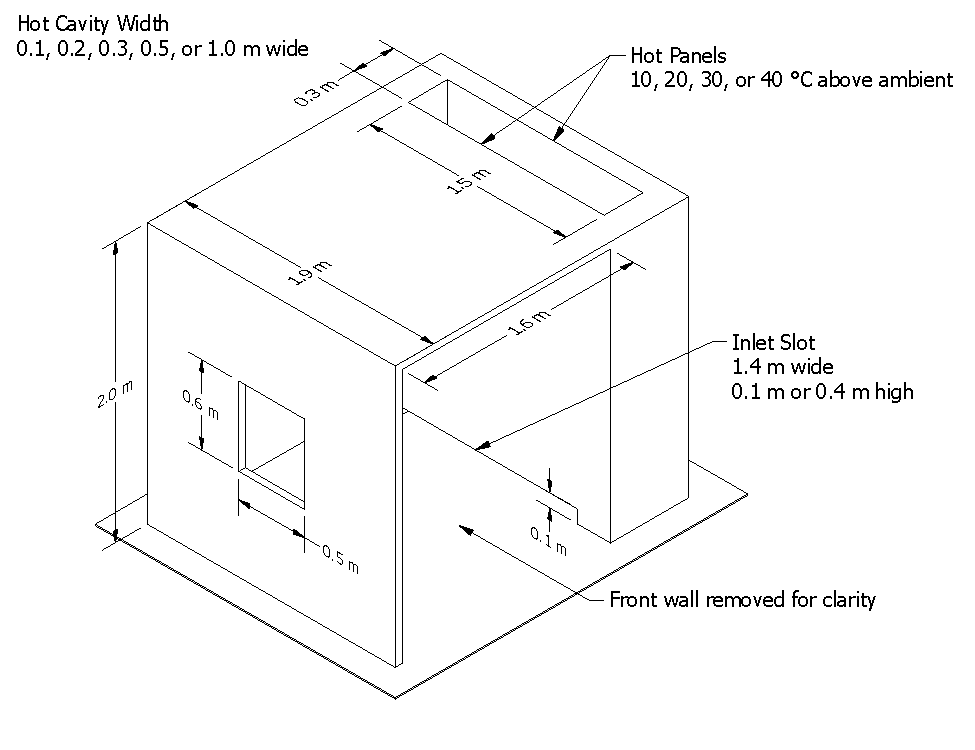
\includegraphics[trim={16in 2.5in 16in 2.5in},clip,width=\textwidth]{FIGURES/Bouchair_Solar_Chimney/Bouchair_Solar_Chimney}
\caption[Geometry of the Bouchair Solar Chimney experiment]{Geometry of the Bouchair Solar Chimney experiment.}
\label{Bouchair_Drawing}
\end{figure}


\section{BRE Spray Test for Radiation Attenuation}
\label{BRE_Spray_Description}

Murrel et al.~\cite{Murrel:1995} measured the attenuation of thermal radiation passing through a water
spray using a heat flux gauge. The radiation was produced by a heat panel, one meter square, at 900~$^\circ$C. The horizontal distance
from the radiation panel to the spray nozzle was 2 m and to the measurement point 4 m. The nozzles were positioned at
a height 0.24 m above the panel upper edge. The heat flux gauge was positioned at the line passing through the center
of the panel. The attenuation of radiation was defined as $(q_0-q_s)/q_0$, where $q_0$ is the initial radiative heat flux,
measured without a spray, and $q_s$ is the heat flux measured during the spray operation.

Experimental results are used from three full-cone type nozzles, labeled A, B and D. The opening angles of the nozzles were between 90 and 108 degrees.
The purpose of the simulation is to compare the measured and simulated attenuation of radiation at different flow conditions. The nozzles were
specified in terms of median droplet size and mean vertical velocity using PDPA measurement in a single position, 0.7 m below the nozzle. The droplet
boundary conditions were determined by assuming $d_m \propto p^{-1/3}$ and $v \propto p^{1/2}$ type of dependencies between the droplet size, speed
and pressure.

\section{Bryant Doorway Velocity Measurements}
\label{Bryant_Doorway_Velocity_Description}

Rodney Bryant of the Fire Research Division at NIST performed a series of velocity measurements of the gas velocity within the doorway of a standard ISO~9705 compartment for fires ranging from 34~kW to 511~kW~\cite{Bryant:FSJ2009,Bryant:EF2009,Bryant:CS2010}. A doorway served as the only vent for the enclosure. It included a jamb of 37~cm extending outward to facilitate the laser measurements. The entire compartment was elevated 0.3~m off the floor of the laboratory (see Fig.~\ref{Bryant_Drawing}). The measurements were made using both bi-directional probes and PIV (Particle Image Velocimetry). The PIV measurements only cover the
lower two-thirds of the doorway because of difficulties in seeding the hot outflow gases. The bi-directional probe measurements span the entire height of the doorway, but Bryant reports that these measurements were up to 20~\% greater than the PIV measurements in certain regions of the flow. Consequently, only the PIV data was used for comparison to the model.

\begin{figure}[ht]
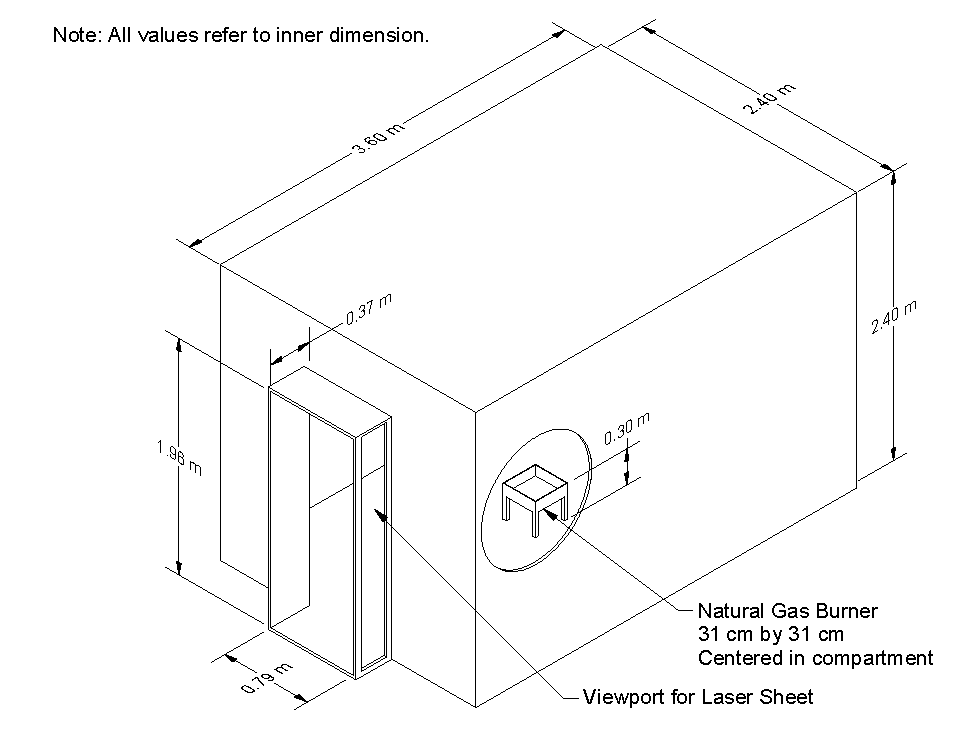
\includegraphics[width=\textwidth]{FIGURES/Bryant_Doorway/Bryant_Compartment}
\caption[Geometry of Bryant's compartment]{Geometry of Bryant's compartment.}
\label{Bryant_Drawing}
\end{figure}

\section{BST/FRS Wood Crib Fire Experiments}
\label{BST_FRS_wood_cribs_description}

In 1993, British Steel Technical, Swinden Laboratories, in collaboration with the Building Research Establishment (BRE), Fire Research Station, conducted nine fire experiments inside the BRE ex-airship hangar testing facility at Cardington, Bedfordshire, England~\cite{BST_FRS:1994}. The objective of the experiments was to examine the influence of combustible loading and ventilation on fire severity.

The roof of the test compartment was made of 20~cm thick reinforced aerated concrete slabs with a density of 450~kg/m$^3$. The walls were made of 215~mm thick lightweight concrete blocks with a density of 1375~kg/m$^3$. The floor was covered with a 125~mm deep layer of sand with a density of 1750~kg/m$^3$. Both the roof and walls were lined with two 25~mm thick layers of standard grade ceramic fiber blanket with a density of 128~kg/m$^3$. Taking into account the lining materials, the compartment was 22.9~m long, 5.6~m deep, and 2.8~m high.

Ventilation was provided at one end of the compartment through a full-width, variable height opening. Lightweight concrete blocks were used to construct temporary walls to reduce the ventilation from fully open to an eighth of the available area.

The combustibles consisted of 33 1~m square wood cribs in 11 rows. Each crib was constructed of 1~m long and 5~cm square cross section sticks of Western Hemlock softwood ( density 400~kg/m$^3$), dried to 10~\% moisture content. The sticks were stacked with 5~cm gaps. Table~\ref{BST_FRS_wood_cribs_tests} lists the fire load densities and ventilation areas. The rear-most three cribs at the back of the compartment were ignited simultaneously. Temperatures were measured along crib lines 2 (back), 6 (middle) and 10 (front), using 3~mm thermocouples placed 300~mm below the ceiling. The average of three thermocouples at the same longitudial position is used for model validation.

\begin{table}[ht]
\begin{center}
\caption[BST/FRS test cases]{Fire load densities and relative ventilation areas in the BST/FRS experiments~\cite{BST_FRS:1994}.}
\label{BST_FRS_wood_cribs_tests}
\begin{tabular}{|l|c|c|c|c|c|c|}
\hline
Test number                     & 1   & 2   & 3   & 4   & 5  & 6  \\ \hline \hline 
Combustible load (kg/m$^2$)     & 40  & 20  & 20  & 40  & 20 & 20 \\
Relative Ventilation Area       & 1/1 & 1/1 & 1/2 & 1/2 & 1/4 & 1/8 \\ \hline
\end{tabular}
\end{center}
\end{table}

\subsubsection{Modeling Notes}

The fire spread on wood cribs is modeled as a combination of simple and complex pyrolysis models. The unresolved surface area of the wood cribs is compensated using a area multiplicator input parameter. Modeling is reported in~\cite{Janardhan:FSJ2021}.


\section{Cable Response to Live Fire -- CAROLFIRE}
\label{CAROLFIRE_Description}

CAROLFIRE was a project sponsored by the U.S.~Nuclear Regulatory Commission to study the thermal response and functional behavior of electrical cables~\cite{CAROLFIRE}. The primary objective of CAROLFIRE was to characterize the various modes of electrical failure (e.g., hot shorts, shorts to ground) within bundles of power, control and instrument cables. A secondary objective of the project was to develop a simple model to predict \underline{th}ermally-\underline{i}nduced \underline{e}lectrical \underline{f}ailure (THIEF). The measurements used for these purposes were conducted at Sandia National Laboratories and are described in Volume II of the CAROLFIRE test report. In brief, there were two series of experiments. The first were conducted within a heated cylindrical enclosure. Single and bundled cables were exposed to various heat fluxes and the electrical failure modes recorded. The second series of experiments involved cables within trays in a semi-enclosed space under which a gas-fueled burner created a hot layer to force cable failure. Only results from the first series are used here.

Petra Andersson and Patrick Van Hees of the Swedish National Testing and Research Institute (SP) proposed that a cable's thermally-induced electrical failure can be predicted via a one-dimensional heat transfer calculation, under the assumption that the cable can be treated as a homogenous cylinder~\cite{Andersson:2005}. Their results for PVC cables were encouraging and suggested that the simplification of the analysis is reasonable and that it should extend to other types of cables. The assumptions underlying the THIEF model are as follows:
\begin{enumerate}
\item The heat penetration into a cable of circular cross section is primarily in the radial direction.
\item The cable is homogeneous in composition. In reality, a cable is constructed of several different types of polymeric materials, cellulosic fillers, and a conducting metal, most often copper.
\item The thermal conductivity, specific heat, and density of the assumed homogeneous cable are independent of temperature. In reality, both the thermal conductivity and specific heat of polymers are temperature-dependent, but this information is not easily obtained from manufacturers.
\item It is assumed that no decomposition reactions occur within the cable during its heating, and ignition and burning are not considered in the model. In fact, thermoplastic cables melt, thermosets form a char layer, and both release volatile gases up to and beyond the point of electrical failure.
\item Electrical failure occurs when the temperature just inside the cable jacket reaches an experimentally determined value.
\end{enumerate}



\section{Crown Fires}
\label{Crown_Fires_Description}

The term ``crown fire'' refers to a wildfire that spreads from the ground surface into the tree canopy. Alexander and Cruz~\cite{Alexander:CJFR2006} compiled a data set of 57 crown fires that occurred in the U.S. and Canada between 1965 and 2003. For each fire, the relative humidity, ambient temperature, and dominant vegetation type are reported, along with estimated values for the vegetation moisture content, {\em canopy}\footnote{Note the difference between {\em canopy} bulk density and {\em crown} bulk density, both of which are abbreviated CBD. The former is the bulk density over the entire forested area, whereas the latter refers to the bulk density within the crown of an individual tree.} bulk density, and open 10~m wind speed. The vegetation consists mainly of coniferous trees, like pines and spruces, and dry undergrowth and ground cover, i.e. scrub brush and dry pine needles. The reported relative humidity ranges between 5~\% and 50~\%, the estimated moisture content ranges between 5~\% and 10~\%, the estimated {\em canopy} bulk density ranges between 0.1~kg/m$^3$ and 0.2~kg/m$^3$, the estimated wind speed ranges between 10~km/h and 50~km/h, and the observed rate of spread ranges between 10~m/min and 110~m/min.

\subsubsection{Modeling Notes}

It is not possible to compare directly the model simulations with the observed fires because of lack of information about the number, spacing, and height of the trees; and the depth, mass, and composition of the ground cover. Instead, Ziegler~et~al.~\cite{Ziegler:thesis,Ziegler:FEM2017,Ziegler:Data2019,Hoffman:FT2016} developed tree maps based on various forests found in the western region of the U.S. The maps contain the location and rough dimensions of each tree in a 4~ha area. Eight maps were developed based on four specific locations and pre- or post-treated conditions. In addition, Ziegler~et~al.~suggest that the moisture content of the trees is approximately 100~\%, and the ground cover 5~\%. The {\em crown} bulk density for all simulations is 1.2~kg/m$^3$, and the surface density is 0.72~kg/m$^2$ with a depth of 6~cm. The simulated fires are ignited along a strip, and the rate of spread is calculated based on the position of peak temperature.

The simulations are performed with a numerical grid that has a resolution of 1~m by 1~m by 0.5~m near the ground, and the vertical dimension increases gradually with height. Because of this relatively coarse resolution, the burning rate of the vegetation is limited to ensure that any given patch of surface vegetation or volume of canopy vegetation cannot burn completely in less than 30~s.





\section{CSIRO Grassland Fires}
\label{CSIRO_Grassland_Fires_Description}

In July and August of 1986, the Commonwealth Scientific and Industrial Research Organisation (CSIRO) of Australia conducted controlled grassland fire experiments near Darwin, Northern Territory~\cite{Cheney:IJWF1993}. July and August are in the middle of the dry season when the grasses are fully cured (dried) and the weather is warm and dry. The experiments were conducted on flat plots measuring 100~m by 100~m, 200~m by 200~m, or 200~m by 300~m. Two cases have been simulated. Case~C064 was conducted on a 100~m by 100~m plot of kerosene grass ({\it Eriachne burkittii}); Case~F19 was conducted on a 200~m by 200~m plot of kangaroo grass ({\it Themeda australis}).

\subsubsection{Modeling Notes}

Two of these experiments were originally simulated with FDS by Mell~et~al.~\cite{Mell:IJWF2007}. These simulations modeled the grass as a collection of cylindrical Lagrangian particles. The pyrolysis model assigned to the particles is described in the FDS User's Guide~\cite{FDS_Users_Guide}, chapter ``Earth, Wind and Fire,'' Section~\ref{UG-vegetation_model}, ``Thermal Degradation Model for Vegetation.''

Now these two experiments are also simulated using the Boundary Fuel Model (BFM)~\cite{Perez-Ramirez:FT2017} and the Rothermel-Albini fire spread algorithm~\cite{Rothermel:1972,Albini:1976}. For the experiment labelled Case~C064, fuel index 1 (Short Grass) is used, with a modified moisture fraction of 0.063. For F19, fuel index 3 (Tall Grass) is used, with a modified moisture fraction of 0.058.

Measured properties for the specific types of grasses burned in the two experiments are listed in Table~\ref{Properties_Grasses}. Properties that were not measured are listed in Table~\ref{Assumed_Properties_Grasses}. These assumed properties are typically for wood or cellulosic fuels. The moisture is modeled as water. The grass is assumed to be composed primarily of cellulose.



\begin{figure}[p]
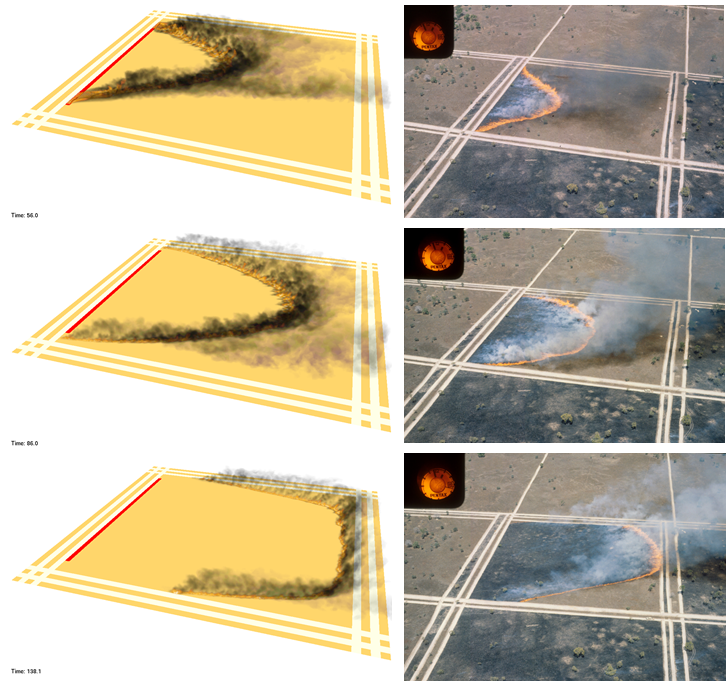
\includegraphics[width=\textwidth]{FIGURES/CSIRO_Grassland_Fires/F19_collage.png}
\caption[Snapshots of the simulation of CSIRO Grassland Fire F19]{Snapshots of the simulation of CSIRO Grassland Fire F19 compared to photographs of the fire.}
\label{F19}
\end{figure}

Snapshots of the Lagrangian particle simulation of Case~F19 is shown in Fig.~\ref{F19}. The computational domain in this case is 240~m by 240~m by 20~m. The grid cells are 0.5~m cubes. The domain is subdivided into 36 individual meshes and run in parallel. The grass is represented 1 simulated blade per grid cell. The radius of the cylinder is derived from the measured surface area to volume ratio. Each simulated blade of grass represents many more actual blades of grass. The weighting factor is determined from the measured bulk mass per unit area. The fires in the experiments were ignited by two men carrying drip torches walking in opposite directions along the upwind boundary of the plot (the red strip in Fig.~\ref{F19}). In FDS, this action was modeled using a specified spread rate along the strip.

\begin{table}[ht]
\begin{center}
\caption[Measured properties for the CSIRO Grassland Fire cases]{Measured properties for the CSIRO Grassland Fire cases~\cite{Cheney:IJWF1993}.}
\label{Properties_Grasses}
\begin{tabular}{|l|c|c|c|}
\hline
Property                        & Units         & Case F19      & Case C064     \\ \hline \hline
Wind Speed                      & m/s           & 4.8           & 4.6           \\ \hline
Ambient Temperature             & $^\circ$C     & 34            & 32            \\ \hline
Surface Area to Volume Ratio    & m$^{-1}$      & 12240         & 9770          \\ \hline
Grass Height                    & m             & 0.51          & 0.21          \\ \hline
Bulk Mass per Unit Area         & kg/m$^2$      & 0.313         & 0.283         \\ \hline
Moisture Fraction               & \%            & 5.8           & 6.3           \\ \hline
\end{tabular}
\end{center}
\end{table}

\begin{table}
\begin{center}
\caption[Assumed properties for dry grass and soil]{Assumed properties for various types of dried grass and soil. Note that the Pyrolysis Temperature is taken to be the temperature at which the mass loss rate peaks in the TGA experiments of Morvan and Dupuy~\cite{Morvan:CF2004}.}
\label{Assumed_Properties_Grasses}
\begin{tabular}{|l|c|c|c|}
\hline
Property                        & Units                 & Value                     & Reference                             \\ \hline \hline
Chemical Composition            & --                    & C$_6$H$_{10}$O$_5$        & Assumption                            \\ \hline
Heat of Combustion              & kJ/kg                 & 15600                     & \cite{Susott:FS1982}                  \\ \hline
Soot Yield                      & kg/kg                 & 0.015                     & \cite{SFPE:Tewarson}                  \\ \hline
Char Yield                      & kg/kg                 & 0.2                       & \cite{Susott:FS1982}                  \\ \hline
Specific Heat                   & kJ/(kg$\cdot$K)       & 1.5                       & Various sources                       \\ \hline
Conductivity                    & W/(m$\cdot$K)         & 0.1                       & Assumption                            \\ \hline
Density                         & kg/m$^3$              & 512                       & \cite{Rothermel:1972}                 \\ \hline
Heat of Pyrolysis               & kJ/kg                 & 418                       & \cite{Morvan:CF2004}                  \\ \hline
Pyrolyis Temperature            & $^\circ$C             & 200                       & \cite{Morvan:CF2004}                  \\ \hline \hline
Obukhov Length                  & m                     & -500                      & Assumption                            \\ \hline
Aerodynamic Roughness Length    & m                     & 0.03                      & Assumption                            \\ \hline
Drag Coefficient                & --                    & 2.8                       & \cite{Falkenstein-Smith:2018}         \\ \hline \hline
Soil Specific Heat              & kJ/(kg$\cdot$K)       & 2.0                       & \cite{Farouki:1981}                   \\ \hline
Soil Conductivity               & W/(m$\cdot$K)         & 0.25                      & \cite{Farouki:1981}                   \\ \hline
Soil Density                    & kg/m$^3$              & 1300                      & \cite{Farouki:1981}                   \\ \hline

\end{tabular}
\end{center}
\end{table}


\section{CSTB Tunnel Experiments}

Between 2005 and 2008, the French building research laboratory, Centre Scientifique et Technique du B\^{a}timent (CSTB) cooperated with the French Tunnel Study Center (CETU), the French National Centre for Scientific Research (CNRS, Institut PPRIME) and the French Directorate for Civil Security (DSC) to conduct fire experiments in a tunnel, some of which involved a water mist system~\cite{Meyrand,Blanchard:FT2014}. The first aim was to improve the understanding of the interaction between water mist and a tunnel fire.  The second was to develop a database for model validation. A one-third scale was selected with the objective of studying realistic fire phenomena in an affordable way.  Twenty-eight experiments were conducted (20 with and 8 without water mist) with varying fuels (heptane pool, wood crib, and wood pallet) and longitudinal velocities (with and without back layering).

The tunnel was 43~m long, with a semi-circular cross section whose area was approximately 4~m$^2$. The walls were covered by a fire resistant mortar cement with well known thermal properties. The floor was made of concrete. A fan was mounted at the downstream side of the tunnel.  Measurements were made of the following: fuel mass, gas temperature, air velocity, radiative heat flux and gas concentration (CO, CO$_2$ and O$_2$).  Sensors were located at 11 longitudinal positions.

Tests~2 and 27 have been selected because neither exhibited back layering. The longitudinal velocity in Test~2 was approximately 2.2~m/s and in Test 27 it was 3.1~m/s. Both experiments involved a 0.5~m$^2$ area heptane pool. In Test~2, the HRR was deduced from the fuel mass loss rate only.  In Test~27, the HRR was deduced from both the mass loss rate and from oxygen consumption calorimetry.

In Test 27, a water mist system was manually activated 300~s after ignition. The water mist system was composed of six nozzles along the centerline of the tunnel, from 4~m upstream to 3.5~m downstream of the fire, 1.5~m apart.  The operating pressure was approximately 90~bar. The water flow rate injected at each nozzle was close to 5.5~L/min, corresponding to a total mist discharge rate of approximately 33~L/min.  Test~27 is interesting because it involved a very low water injection rate.  The main consequence is that the HRR actually increased slightly after the nozzles were activated, and the fire did not extinguish.  The experiment stopped when the fuel was exhausted. This allowed for an assessment of the model's ability to predict the gas cooling and radiation attenuation.

\subsubsection{Modeling Notes}

The simulations of these experiments are performed using 12 meshes. To prevent numerical instability due to oscillations in pressure, a common problem for tunnel fire simulations, the {\ct VELOCITY\_TOLERANCE} and {\ct PRESSURE\_TOLERANCE} are reduced to 0.01~m/s and 400~s$^{-2}$, respectively, and the {\ct MAX\_PRESSURE\_ITERATIONS} is increased to 50. The multi-port mist nozzles are each modeled as a collection of single nozzles with varying orientations.



\section{Cup Burner Experiments}
\label{Cup_Burner_Description}

The cup-burner is a widely used experimental apparatus for studying the effectiveness of flame extinguishing agents. Typically, these experiments feature a steady fuel-air co-flow diffusion flame that is established above the cup. The extinguishing agent is gradually introduced into the air stream to determine the minimum concentration of the agent that leads to lift off. One hundred and ten experimental data sets are examined. The data sets include sixteen fuels: acetone, acetylene, benzene, butane, dodecane, ethanol, ethylene, heptane, hexane, hydrogen, methane, methanol, octane, propanol, and toluene, and five inert gases: argon (Ar), carbon dioxide (CO$_2$), helium (He), and nitrogen (N$_2$), and sulfur hexaflouride (SF$_6$). A STANJAN\footnote{STANJAN is a program for chemical equilibrium calculations.} calculation has been performed to determine the equilibrium temperature using the measured minimum extinguishing concentration for each experiment. The calculation assumes constant pressure and enthalpy using a stoichiometric mixture of fuel and air plus agent. For combinations of fuel and agent with multiple experiments, the average extinguishing concentration and the average flame temperature is taken, resulting in forty-six unique combinations of fuel and agent listed in Table~\ref{Cup_Table}.

\begin{table}[p]
\caption{Summary of Cup Burner Data}
\label{Cup_Table}
\small
\begin{tabular}{|l|c|c|c|c|l|}
\hline
Fuel       &  Agent  & MEC  & CFT  & References   \\ \hline \hline
Acetone    & Ar      & 34.0 & 1729 & \cite{Tapscott:1,Moore:1}  \\ \hline
Acetone    & CO$_2$  & 19.0 & 1678 & \cite{Yamamoto:1}  \\ \hline
Acetone    & N$_2$   & 28.0 & 1670 & \cite{Tapscott:1,Yamamoto:1}  \\ \hline
Acetylene  & CO$_2$  & 45.0 & 1338 & \cite{Yamamoto:1}  \\ \hline
Acetylene  & N$_2$   & 58.0 & 1312 & \cite{Yamamoto:1}  \\ \hline
Benzene    & CO$_2$  & 20.1 & 1691 & \cite{Yamamoto:1,Sakei:1}  \\ \hline
Benzene    & N$_2$   & 30.3 & 1683 & \cite{Tapscott:1,Yamamoto:1,Sakei:1}  \\ \hline
Butane     & N$_2$   & 31.0 & 1594 & \cite{Yamamoto:1}  \\ \hline
Butane     & CO$_2$  & 19.0 & 1639 & \cite{Yamamoto:1}  \\ \hline
Dodecane   & N$_2$   & 33.0 & 1577 & \cite{Tapscott:1}  \\ \hline
Ethanol    & Ar      & 36.5 & 1654 & \cite{Tapscott:1,Moore:1}  \\ \hline
Ethanol    & CO$_2$  & 23.7 & 1542 & \cite{Yamamoto:1,Sakei:1}  \\ \hline
Ethanol    & N$_2$   & 34.6 & 1529 & \cite{Tapscott:1,Yamamoto:1,Sakei:1}  \\ \hline
Ethylene   & CO$_2$  & 32.0 & 1471 & \cite{Yamamoto:1}  \\ \hline
Ethylene   & N$_2$   & 45.0 & 1441 & \cite{Yamamoto:1}  \\ \hline
Heptane    & Ar      & 39.5 & 1643 & \cite{Tapscott:1,Bogdan:1,Moore:1,Sheinson:FSJ,Grosshandler:Cup,Saito:FSJ,NFPA_2001,ISO_14520,Senecal:FSJ}  \\ \hline
Heptane    & N$_2$   & 31.2 & 1617 & \cite{Tapscott:1,Bogdan:1,Hamins:CS1998,Moore:1,Hirst:1,Sheinson:FSJ,Grosshandler:Cup,Saito:FSJ,Yamamoto:1,Sakei:1,NFPA_2001,ISO_14520,Senecal:FSJ}  \\ \hline
Heptane    & CO$_2$  & 21.4 & 1617 & \cite{Moore:1,Hirst:1,Sheinson:FSJ,Grosshandler:Cup,Saito:FSJ,Yamamoto:1,Sakei:1}  \\ \hline
Heptane    & He      & 31.5 & 1763 & \cite{Sheinson:FSJ,Grosshandler:Cup}  \\ \hline
Heptane    & SF$_6$  & 11.0 & 1531 & \cite{Sheinson:FSJ}  \\ \hline
Hexane     & Ar      & 33.0 & 1740 & \cite{Moore:1}  \\ \hline
Hexane     & CO$_2$  & 20.0 & 1647 & \cite{Yamamoto:1}  \\ \hline
Hexane     & N$_2$   & 29.0 & 1646 & \cite{Tapscott:1,Yamamoto:1}  \\ \hline
Hydrogen   & CO$_2$  & 60.0 &  913 & \cite{Yamamoto:1}  \\ \hline
Hydrogen   & N$_2$   & 72.0 &  870 & \cite{Yamamoto:1}  \\ \hline
Methane    & Ar      & 33.8 & 1659 & \cite{Tapscott:1,Takahashi:CS2007,Moore:1}  \\ \hline
Methane    & N$_2$   & 24.2 & 1663 & \cite{Takahashi:CS2007,Yamamoto:1,Ural:1}  \\ \hline
Methane    & CO$_2$  & 14.4 & 1694 & \cite{Yamamoto:1,Sakei:1}  \\ \hline
Methane    & He      & 26.7 & 1746 & \cite{Takahashi:CS2007}  \\ \hline
Methanol   & Ar      & 45.0 & 1494 & \cite{Tapscott:1,Moore:1}  \\ \hline
Methanol   & CO$_2$  & 29.2 & 1410 & \cite{Yamamoto:1,Sakei:1}  \\ \hline
Methanol   & N$_2$   & 40.8 & 1395 & \cite{Tapscott:1,Yamamoto:1,Sakei:1}  \\ \hline
Octane     & Ar      & 27.0 & 1790 & \cite{Moore:1}  \\ \hline
Octane     & CO$_2$  & 24.0 & 1542 & \cite{Yamamoto:1}  \\ \hline
Octane     & N$_2$   & 33.0 & 1564 & \cite{Tapscott:1,Yamamoto:1}  \\ \hline
Propane    & Ar      & 37.5 & 1652 & \cite{Tapscott:1,Moore:1}  \\ \hline
Propane    & CO$_2$  & 21.0 & 1600 & \cite{Yamamoto:1}  \\ \hline
Propane    & N$_2$   & 32.3 & 1573 & \cite{Hamins:CS1998,Yamamoto:1,Ural:1}  \\ \hline
Propanol   & Ar      & 28.0 & 1781 & \cite{Moore:1}  \\ \hline
Propanol   & CO$_2$  & 22.0 & 1584 & \cite{Yamamoto:1}  \\ \hline
Propanol   & He      & 30.0 & 1755 & \cite{Sheinson:FSJ}  \\ \hline
Propanol   & N$_2$   & 30.0 & 1608 & \cite{Yamamoto:1,Sheinson:FSJ}  \\ \hline
Propanol   & SF$_6$  & 11.0 & 1515 & \cite{Sheinson:FSJ}  \\ \hline
Toluene    & Ar      & 27.0 & 1854 & \cite{Moore:1}  \\ \hline
Toluene    & CO$_2$  & 17.0 & 1744 & \cite{Yamamoto:1,Sakei:1}  \\ \hline
Toluene    & N$_2$   & 24.4 & 1755 & \cite{Yamamoto:1,Sakei:1}  \\ \hline
\end{tabular}
\noindent
\begin{tabbing}
MEC  \hspace{0.05in} \= Minimum Extinguishing Concentration (mol/mol) \\
CFT                  \> Critical Flame Temperature ($^\circ$C)
\end{tabbing}
\end{table}


\subsubsection{Modeling Notes}

Cup burner dimensions, fuel inlet velocity, and co-flow inlet velocity vary slightly amongst the researchers; however, extinguishing concentrations have been shown to be fairly insensitive over the range of typical values. The cup burner model was implemented as a 2D, cylindrical geometry with a 1 cm radius for the burner and a 4 cm radius for the tube. A 1 mm grid resolution was used. For gaseous fuels a 1 cm/s inlet velocity was used for the burner. Liquid fuels used burning rates from the SFPE Handbook; fuels without published burning rates scaled the burning rate of a chemically similar fuel (e.g. alcohol, alkane) using the heat of vaporization for the fuel. The fuel temperature boundary condition was ambient for gaseous fuels and one-half of the boiling point for liquid fuels. The co-flow was set to 12~cm/s. The agent mass fraction was ramped from approximately 10~\% below to 10~\% above the values shown in Table~\ref{Cup_Table}. The {\ct CRITICAL\_FLAME\_TEMPERATURE} was set to the values in Table~\ref{Cup_Table}.

\section{DelCo Trainer Experiments}
\label{DelCo_Description}

The NIST Fire Fighting Technology Group conducted a series of experiments in two structures of similar design located at the Delaware County (``DelCo'') Emergency Services Training Center in Sharon Hill, Pennsylvania~\cite{DelCo_TN}. Three propane burners were used to provide the fire source for all experiments, and various sensors were used to collect gas temperature, gas velocity, heat flux, and gas concentration measurements throughout the structure.

The single level structure was instrumented with five bare-bead thermocouple arrays and two gas sample inlet pipes at the locations shown in Fig.~\ref{fig:east_instrumentation}. Both floors of the two level structure were instrumented with three bare-bead thermocouple arrays and one gas sample inlet pipe at the locations shown in Fig.~\ref{fig:west_instrumentation}.

\begin{figure}[!ht]
\includegraphics[width=\columnwidth]{FIGURES/DelCo_Trainers/East_Structure_Dimensioned_Instrumentation}
\caption[Instrumentation of the single level DelCo training structure]{Instrumentation of the single level DelCo training structure. The thermocouple arrays are denoted by crossed circles and the gas sampling measurement locations are denoted by hexagons at locations A1 and A4. The burner is denoted by three cross-hatched squares.}
\label{fig:east_instrumentation}
\end{figure}

\begin{figure}[p]
\includegraphics[width=0.94\columnwidth]{FIGURES/DelCo_Trainers/West_Structure_2nd_Floor_Dimensioned_Instrumentation}
\\~\\
\includegraphics[width=\columnwidth]{FIGURES/DelCo_Trainers/West_Structure_1st_Floor_Dimensioned_Instrumentation}
\caption[Instrumentation of the two level DelCo training structure]{Instrumentation of the second floor (top) and first floor (bottom) of the two level DelCo training structure. The thermocouple arrays are denoted by crossed circles and the gas sampling measurement locations are denoted by hexagons at locations A1 and A10. The burner is denoted by three cross-hatched squares.}
\label{fig:west_instrumentation}
\end{figure}


\section{DoJ/HAI Pool Fire Experiments}
\label{DoJ_HAI_Pool_Fires_Description}

The U.S. Department of Justice sponsored a series of liquid pool fire experiments performed by Hughes Associates, Inc.~\cite{Mealy:DoJ_HAI_Pool_Fires}. Hundreds of experiments were performed, involving six different liquid fuels, eight different substrates, a variety of pan sizes and pool depths. Of these, 44 experiments were chosen from the ``Diked Fire Test Series,'' where gasoline or kerosene was burned within 0.3~m, 0.6~m, or 1.2~m square pans with liquid depths ranging from 1~mm to 20~mm. The substrate was either coated concrete or vinyl, each of which was designed to avoid liquid absorption. The vinyl flooring material had a nominal thickness of 1.2~mm applied to a 14.7~mm plywood using a vinyl adhesive. Table~\ref{DoJ_HAI_Matrix} provides a summary of the experimental parameters.

\subsubsection{Modeling Notes}

The test report for the experiments does not explicitly list the components of the gasoline or kerosene. Rather, distillation curves are provided showing that the initial and final boiling points for gasoline are 45~$^\circ$C and 212~$^\circ$C, and for kerosene 170~$^\circ$C and 257~$^\circ$C. The density of the gasoline is 742~kg/m$^3$ and the kerosene 798~kg/m$^3$. From various industry documents, it is postulated that the gasoline is a mixture of n-hexane (0.521 by mass), n-heptane (0.054), n-octane (0.063), n-decane (0.023), benzene (0.20), and toluene (0.139). The kerosene is assumed to be a mixture of iso-octane (0.04), n-nonane (0.19), iso-nonane (0.12), n-decane (0.15), iso-decane (0.11), n-undecane (0.09), and cis-decalin (0.30). The relavant properties of these liquids are listed in Table~\ref{fuelprops}.

A few additional assumptions are made concerning the mixtures. First, that the absorption coefficient of all components is set to 150~m$^{-1}$, a value that is typical of heavy hydrocarbon liquids. Seconds, the thermal conductivity of the components is set to an artificially low value of 0.02~W/m/K to roughly account for the buoyancy that drives heated liquid upwards towards the surface. Third, all liquid components are assumed to evaporate into a single gas phase species, n-hexane. If this were not assumed, additional transport equations and combustion reactions would be needed for all liquid components.

Finally, to simulate the ignition of the liquid pools, an external flux is imposed at the surface for 10~s in the case of gasoline and 25~s for kerosene.
 
\begin{table}[h!]
\begin{center}
\caption[Gasoline and kerosene components]{Gasoline and kerosene components~\cite{CRCHandbook:Enthalpy_of_Vaporization}.} 
\label{fuelprops2}
\begin{tabular}{|l|c|c|c|c|c|c|} \hline
Fuel        & Chemical          & $W$         & $\rho$      & $c_p$              & $h_{\rm v}$        & $T_{\rm b}$     \\
Component   & Formula           & (g/mol)     & (kg/m$^3$)  & (kJ/(kg$\cdot$K))  & (kJ/kg)            & $^\circ$C       \\
\hline \hline
Benzene     & C$_6$H$_{6}$      & 78.1        & 879         & 1.72              & 393                 & 80.1   \\ \hline
cis-Decalin & C$_{10}$H$_{18}$  & 138.3       & 897         & 1.68              & 297                 & 195.8  \\ \hline
iso-Decane  & C$_{10}$H$_{22}$  & 142.3       & 728         & 2.20              & 269                 & 167.0  \\ \hline
n-Decane    & C$_{10}$H$_{22}$  & 142.3       & 730         & 2.21              & 278                 & 174.1  \\ \hline
n-Heptane   & C$_7$H$_{16}$     & 100.2       & 684         & 2.24              & 317                 & 98.4   \\ \hline
n-Hexane    & C$_6$H$_{14}$     & 86.2        & 659         & 2.27              & 335                 & 68.7   \\ \hline
iso-Nonane  & C$_9$H$_{20}$     & 128.3       & 708         & 2.34              & 350                 & 143.0  \\ \hline
n-Nonane    & C$_9$H$_{20}$     & 128.3       & 718         & 2.22              & 290                 & 150.8  \\ \hline
iso-Octane  & C$_8$H$_{18}$     & 114.2       & 692         & 2.09              & 270                 & 99.2   \\ \hline
n-Octane    & C$_8$H$_{18}$     & 114.2       & 702         & 2.23              & 301                 & 125.6  \\ \hline
Toluene     & C$_7$H$_{8}$      & 92.1        & 867         & 1.67              & 360                 & 110.6  \\ \hline
n-Undecane  & C$_{11}$H$_{24}$  & 156.3       & 740         & 2.21              & 268                 & 195.9  \\ \hline
\end{tabular}
\end{center}
\end{table}


\section{Droplet Evaporation}
\label{Droplet_Evaporation_Description}

Five sets of experiments have been selected for validation of the evaporation of liquid droplets.

\subsubsection{Fujita, Kurose, and Komori Experiments}
\label{Fujita_exp}

Fujita, Kurose, and Komori performed a series of experiments that suspended a water drop in a heated, vertical wind tunnel~\cite{Fujita}. Four experiments were modeled with relative humidity values of 0~\% and 30~\% and droplet Reynolds numbers of 60 and 150 (approximately 0.8~m/s and 2.0~m/s). Droplet size and surface temperature were recorded as functions of time.

\subsubsection{Gavin Experiments}
\label{Gavin_exp}

Gavin performed two experiments of a single water drop falling in dry air~\cite{Gavin}. The test apparatus was a vertical wind tunnel. A drop was injected into the wind tunnel and the vertical air stream velocity was changed over time to maintain the drop at a constant elevation in the wind tunnel. The first droplet was 769~$\mu$m with an initial temperature of 23.0~$^\circ$C. The second droplet was 557~$\mu$m with an initial temperature of 24.3~$^\circ$C.

\subsubsection{Kolaitis and Founti Experiments}
\label{Kolaitis_exp}

Kolaitis and Founti measured the diameter and temperature of suspended liquid fuel droplets in a heated air stream~\cite{Kolaitis}. Four experiments were chosen: a 1.26~mm droplet of ethanol at an initial temperature of 34.2~$^\circ$C in 94~$^\circ$C quiescent air, a 1.13~mm droplet of decane at an initial temperature of 73.8~$^\circ$C in 94~$^\circ$C quiescent air, a 1.15~mm droplet of heptane at an initial temperature of 49.0~$^\circ$C in 94~$^\circ$C quiescent air, and a 1.42~mm droplet of heptane at an initial temperature of 15.5~$^\circ$C in 94~$^\circ$C air at 0.146~m/s.

\subsubsection{Maqua, Castanet, and Lemoine Experiments}
\label{Maqua_exp}

Maqua, Castanet, and Lemoine measured the temperature of falling droplets of ethanol and acetone mixtures in a heated plume~\cite{Maqua}. Because the temperature and velocity of the plume was not well-characterized, only the experiments involving a droplet falling in quiescent air were modeled. As FDS does not currently have a sub-model for the evaporation of a multi-component fuel, only the experiments for a pure ethanol droplet (140~$\mu$m) and a pure acetone droplet (140~$\mu$m) were modeled. The initial droplet temperature in both experiments was 45~$^\circ$C in 20~$^\circ$C air.

\subsubsection{Taflin Experiments}
\label{Taflin_exp}

Taflin measured the diameter of suspended water droplets in dry air~\cite{Snegirev:1}. One droplet was initially 43.9~$\mu$m and the other was 56.6~$\mu$m.

\section{Edinburgh Vegetation Drag}
\label{Edinburgh_Veg_Drag_Description}

Mueller et al.~\cite{Mueller:TIPM2021} characterized the pressure drop through beds of randomly oriented pine needles and used the results to parameterize a drag model following the form of the Forchheimer equation. They then measured the development of velocity profiles within and above these pine needle beds, using a hotwire anemometer, and compared the results to FDS predictions using the parameterized model. Fuel beds with bulk densities of 20~kg/m$^3$, 40~kg/m$^3$, and 60~kg/m$^3$ were tested, with inlet velocities in the range of 0.5-2.0~m/s. A condensed version of the comparison is reproduced in this guide, which serves to test the ability of the model to represent the general features of flow in sparse multiphase media.

\subsubsection{Modeling Notes}

In the experiment, the test section extended 400~mm beyond the vegetation layer. This extent of the domain is reproduced in the simulations in order to avoid possible influence of the downstream boundary condition. The upstream boundary condition is set using the measurements located at $x=-75$~mm, which allows for the reproduction of a slight non-uniformity in the flowfield. Due to difficulties in compacting the high bulk density case, the fuel layer is set to extend to 55~mm in the 60~kg/m$^3$ simulations.

\begin{figure}[ht]
\centering
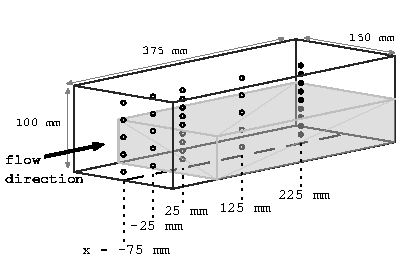
\includegraphics[width=0.5\textwidth]{FIGURES/Edinburgh_Vegetation_Drag/domain_schematic}
\caption[Geometry of the Edinburgh Vegetation Drag experiments]{Geometry of the wind tunnel test section for the Edinburgh Vegetation Drag experiments. Vegetation filled the lower half of the 150~mm x 100~mm test section, starting from $x=0$~mm. Circles indicate the locations of velocity measurements, with the filled circles corresponding to those used for comparison in this guide.}
\label{Ed_Veg_Drag_Layout}
\end{figure}

\section{FAA Cargo Compartments}
\label{FAA_Cargo_Description}

The U.S.~Federal Aviation Administration (FAA) has sponsored experiments and modeling of smoke transport within aircraft storage compartments~\cite{FAA-AR-03-49,FAA-AR-07-27}. Two types of compartments were used; one from a Boeing~707 and one from a McDonnell Douglas DC-10. The 707 compartment was 6.7~m in length, 3.2~m in width, and 1.4~m in height. The DC-10 compartment was 14~m in length, 4.4~m in width, and 1.7~m in height. The fire for all experiments was fueled by a 0.1~m by 0.1~m tray of plastic resin producing a peak HRR of 5~kW~\cite{FAA-AR-06-21}. The long walls of the compartments were barrel-shaped to conform to the shape of the aircraft fuselage. The fire was placed in different locations, and measurements of gas and ceiling temperature, heat flux, gas concentration, and smoke obscuration were made at a variety of locations, mostly near the ceiling.


\section{FAA Polymers}
\label{FAA_Polymers_Description}

As part of their efforts to characterize the burning behavior of commonly used plastics, the U.S.~Federal Aviation Administration (FAA) conducted measurements of the thermal properties of charring and non-charring polymers with the specific purpose of providing input data for numerical pyrolysis models~\cite{Stoliarov:CF2009,Stoliarov:CF2010}. The study aimed to determine whether a one-dimensional conduction/reaction model could be used as a practical tool for prediction and/or extrapolation of the results of fire calorimetry tests. The non-charring polymers included poly(methyl methacrylate) (PMMA), high-impact polystyrene (HIPS), and high density polyethylene (HDPE). The charring polymers included polycarbonate (PC) and polyvinyl chloride (PVC).


\section{Fleury Heat Flux Measurements}
\label{Fleury_Heat_Flux_Description}

Rob Fleury, a master's degree student at the University of Canterbury in Christchurch, New Zealand, measured the heat flux from a variety of propane fires~\cite{Fleury:Masters}. The objective of the work was to evaluate a variety of empirical heat flux calculation methods. For the measurements, heat flux gauges were mounted on moveable dollies that were placed in front of, and to the side of, burners with dimensions of 0.3~m by 0.3~m (1:1 burner), 0.6~m by 0.3~m (2:1 burner), and 0.9~m by 0.3~m (3:1 burner). The heat release rates were set to 100~kW, 150~kW, 200~kW, 250~kW, and 300~kW. The gauges were mounted at heights of 0~m, 0.5~m, 1.0~m, and 1.5~m relative to the top edge of the burner.


\section{FM Burner Experiments}
\label{FM_Burner_Description}

A series of gas burner experiments was conducted by Zeng and Wang at FM Global in which the co-flow air stream was gradually diluted with nitrogen until flame extinction was achieved~\cite{Zeng:26ICDERS}. Numerical simulations were subsequently performed by Ren~et~al.~\cite{Ren:CS2018}. In the experiments, a cylindrical, water-cooled steel burner (15.2~cm O.D., 13.7~cm I.D.) was placed near the floor of a 1.22~m by 1.22~m by 1.83~m tall compartment. Four fuels were used: ethylene (C$_2$H$_4$), methane (CH$_4$), propane (C$_3$H$_8$), and propylene (C$_3$H$_6$). The heat release rate in each experiment was 10~kW with a 1~kW ring of premixed ethylene pilot burners to stabilize the flame. At the start of each experiment, air was pumped through the floor at a rate sufficient to supply the fire with approximately 10 times the stoichiometric requirement. Subsequently, nitrogen was slowly added to the air stream until the fire was extinguished.

In the same enclosure and using the same burner, Ren et al.~\cite{Ren:IAFSS2020} made high-frequency mean and rms temperature measurements along six radial profiles above a 15~kW ethylene fire. Soot measurements were made at similar locations. The co-flow air stream at the floor was set to 20.9~\%, 16.8~\%, and 15.2~\% oxygen volume fraction. Additional experiments were performed at 19~\%, 17~\%, and 15~\% oxygen in which global radiation measurements were made, including total radiative fraction and the vertical distribution of radiative emission.

\subsubsection{Modeling Notes}

The FDS simulations of the 10~kW ethylene, methane, propane and propylene fires are run for 65~s, in which time the oxygen concentration in the co-flow stream is ramped down linearly from 21~\% to 8~\%. The volume flow of the co-flow stream has been increased tenfold compared to the experiments to prevent a downwash of ambient air into the sealed compartment. The 15~kW ethylene fire simulations at the various fixed oxygen levels are performed for 20~s. For these simulations, the oxygen volume fraction is specified directly, as is the co-flow stream.

The 10 kW variable fuel cases examining combustion efficiency and extinction are modeled using a two-step reaction scheme. In the first step, fuel is converted to CO, soot, and water vapor, and in the second step, the CO and Soot are oxidized to form CO$_2$. Both reactions are fast, but the oxidation step follows the first reaction in serial. That is, in a given time step, all available oxygen first converts fuel to CO and Soot, assumed to be C$_{0.9}$H$_{0.1}$. Any leftover oxygen is then used to oxidize existing CO and Soot. There are two assumptions: (i) the ratio of fuel C that is converted to CO in the first reaction step (the remainder goes to Soot) and (ii) the post-flame yields of CO and Soot.  For the first assumption (the intermediate step), we assume that 95 \% of the carbon goes to CO for a clean fuel like methane, we assume 85 \% goes to CO for propane, and that 60 \% goes to CO for both ethylene and propylene.  The post flame yields for each fuel are taken from Tewarson's measurements reported in the SFPE Handbook~\cite{SFPE:Tewarson}.

Under the assumption that Air contains 383~ppm CO$_2$ and water vapor corresponding to 40~\% humidity, the full two-step reaction scheme for ethylene is written in terms of ``lumped'' species as follows:
\begin{eqnarray}
\lefteqn{ \underbrace{\mathrm{ (C_2H_4) }}_\text{Fuel} \; + \;
7.60 \; \underbrace{ \mathrm{\left( 0.208 \, O_2 + 0.783 \; N_2 + 0.0004 \, CO_2 + 0.009 \, H_2O \right)}}_\text{Air} \longrightarrow } \quad \quad \quad \quad \quad \quad \quad \nonumber \\
& & 10.07 \, \underbrace{\mathrm{(0.119 \; CO +  0.201 \; H_2O + 0.088 \; Soot +  0.591\, N_2 + 0.0003 \, CO_2)}}_\text{Products 1}
\end{eqnarray}
\be
(\text{Products 1}) + 0.63 \; (\text{Air}) \longrightarrow  1.49 \, \underbrace{\mathrm{(0.0009 \, CO + 0.0077 \, Soot + 0.126 \, CO_2 +  0.141 \; H_2O  + 0.724 \; N_2)}}_\text{Products 2}
\ee

The pilot ring is modeled with a ``pilot fuel model''.  We use 36 particles arranged in a uniform ring around the burner.  The mass flow rate of ethylene from each particle is set to achieve the total 1 kW from the pilot ring.  In the pilot fuel model, the fuel stream from the pilot particles sees an auto-ignition temperature (AIT) of 0 K.  That is, fuel emanating from the pilot particles is not subject to an ignition temperature threshold.  Further, this fuel undergoes simple 1-step, fast chemistry.  The fuel emanating from the main burner (for each different fuel type, including ethylene) undergoes 2-step, fast chemistry as discussed above and is subject to an ignition temperature threshold with the AIT for each fuel taken from Beyler's chapter in the SFPE Handbook~\cite{SFPE:Beyler}.  Likewise, the critical flame temperatures for each fuel are taken from ~\cite{SFPE:Beyler}.  While there are now 3 chemical reactions for each case (a pilot fuel reaction plus the two main fuel reactions), each with its own ``fuel'', the CFT for the extinction model is based on the fuel for the main burner first step reaction, either methane, ethylene, propylene, or propane.

The burner surface temperature was modeled by specifying a 2.54 cm thick surface made of sand.  The back side temperature was held constant at \SI{25}{\degreeCelsius} to match the water cooled burner in the experiment.

The radiative fraction has been predicted rather than specified in all simulations.

\section{FM/FPRF Data Center Experiments}
\label{FM_FPRF_Datacenter_Description}

The Fire Protection Research Foundation funded a series of large scale tests of smoke detection in high airflow data centers as part of a research project on behalf of the NFPA~75 and NFPA~76 Technical Committees~\cite{FM_Datacenter_Rpt}. The tests consisted of a data center mockup that was 4.9~m high, 4.9~m wide, and 7.3~m deep. The mockup was divided into a 0.9~m tall subfloor with air supplied via a natural vent opening on one short wall, a 0.9~m tall ceiling plenum with air removed via a mechanical vent opening on one short wall, two 2~m tall by 0.6~m wide by 5.3~m long enclosed cold aisles located along the outer walls, and a 3.1~m tall hot aisle.  Flow from the subfloor to the cold aisles occurred through grated floor tiles, flow from the cold aisles to the hot aisle was through two rows of empty equipment cabinets with perforated metal doors, and flow from the hot aisle to the ceiling plenum was through perforated metal ceiling tiles.

Two groups of tests were performed. The first group of tests used a sonic anemometer to map the flow field in the facility for a flow of 78 air changes per hour (ACH) and 265~ACH. Additional measurements were made of the pressure drops through the floor and ceiling tiles. The second group of tests measured smoke detection response to a variety of detectors from a range of typical smoke sources plus propylene (used for its ease of characterization and repeatability).

The FDS model of the facility makes use of the screen drag model for Lagrangian particles to model the pressure losses through the various metal meshes and grates present in the mockup. The FDS model also uses the specified leakage location model to model leakage through the seams of floor and ceiling tiles. The actual leakage area was not measured during the test. Instead the area was estimated using the reduction in the FM measured pressure drop from to the manufacturer's reported pressure drop to compute a leakage flow. A description of the process used to create the FDS model and the test uncertainties can be found in a companion report documenting modeling of the tests with FDS 6.0.0~\cite{FDS_Datacenter_Rpt}.


\section{FM Parallel Panel Experiments}
\label{FM_Parallel_Panel_Description}

Patricia Beaulieu of Worcester Polytechnic Institute made heat flux measurements within a set of vertical parallel panels as part of a cooperative research program between Worcester Polytechnic Institute and FM Global (Factory Mutual)~\cite{Beaulieu:FM}. The experimental apparatus consisted of two vertical parallel panels, 2.4~m high and 0.6~m wide, with a sand burner at the base. The objective of the project was to measure the flame spread rate over various composite wall lining materials, but there were also experiments conducted with inert walls for the purpose of measuring the heat flux from fires fueled by propane and propylene at heat release rates of 30~kW, 60~kW, and 100~kW. A sketch of the apparatus is shown in Fig.~\ref{Parallel_Panel_Sketch}.

\begin{figure}[!ht]
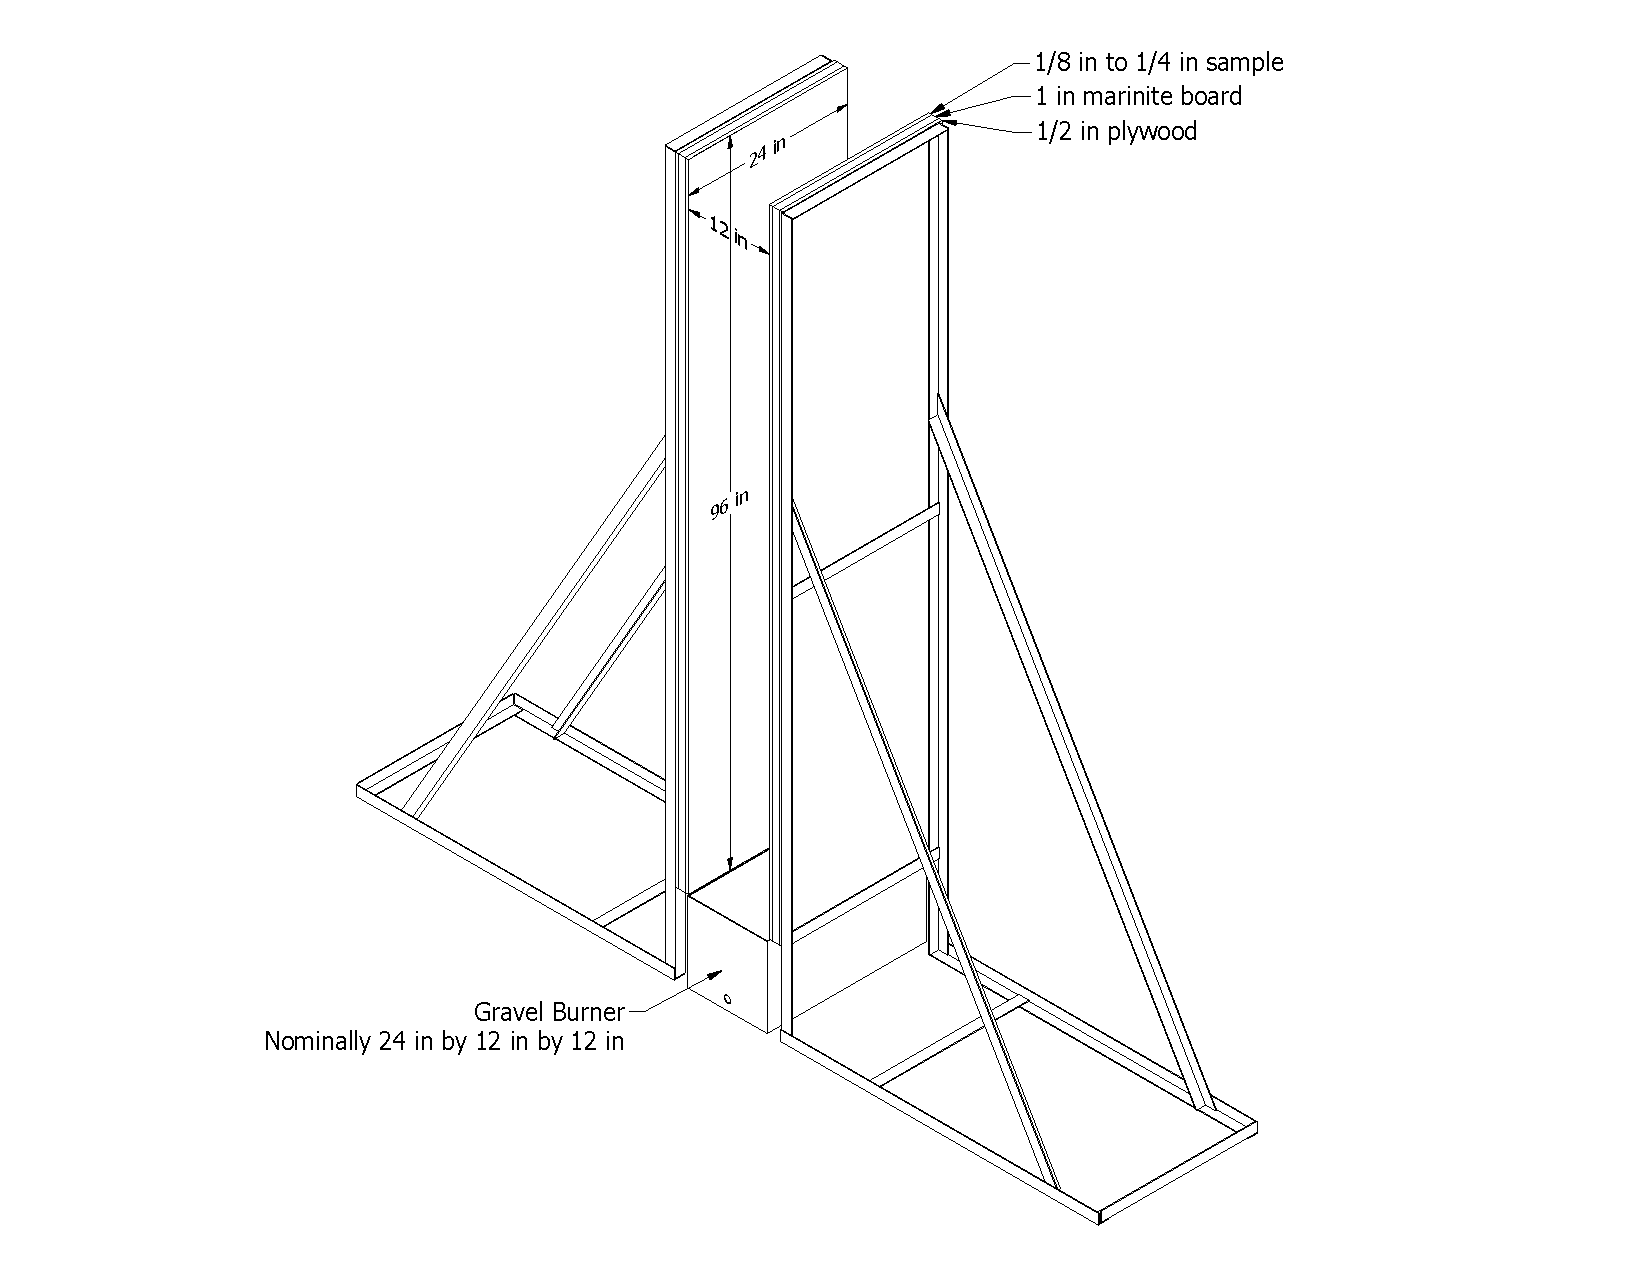
\includegraphics[width=\textwidth]{FIGURES/FM_Parallel_Panel/Full_Assembly}
\caption[Sketch of the FM parallel panel apparatus]{Sketch of the FM parallel panel apparatus.}
\label{Parallel_Panel_Sketch}
\end{figure}



\section{FM/SNL Experiments}
\label{FM_SNL_Description}


The Factory Mutual and Sandia National Laboratories (FM/SNL) test series consists of 25 compartment fire experiments conducted in 1985 for the U.S.~Nuclear Regulatory Commission (NRC) by Factory Mutual Research Corporation (FMRC), under the direction of Sandia National Laboratories (SNL)~\cite{Nowlen:NUREG4681,Nowlen:NUREG4527}. The primary purpose of these experiments was to provide data with which to validate computer models for various types of compartments typical of nuclear power plants. The experiments were conducted in an enclosure measuring approximately 18~m long by 12~m wide by 6~m high, constructed at the FMRC fire test facility in Rhode Island. A drawing is included in Fig.~\ref{FM_SNL_Drawing}. All of the experiments included forced ventilation to simulate typical power plant conditions. Six of the experiments were conducted with a full-scale control room mock-up in place. Parameters varied during the experiments included fire intensity, enclosure ventilation rate, and fire location. Only data from nineteen experiments (Tests 1-17, 21, and 22) is used in the current study. In these experiments, the fires were fueled by a propylene gas burner, and heptane and methanol liquid pools. In the experiments not selected, the heat release was not reported and could not be estimated with confidence. Table~\ref{FM_SNL_Matrix} lists the test parameters.

The following information was provided by the test director, Steve Nowlen of Sandia National Laboratory. In particular, Tests 4, 5, and 21 were given extra attention.
\begin{description}
\item[Heat Release Rate:] The HRR was determined using oxygen consumption calorimetry in the exhaust stack with a correction applied for the carbon dioxide in the upper layer of the compartment. The uncertainty of the fuel mass flow was not documented. Several tests selected for this study had the same target peak heat release rate of 516~kW following a 4~min ``t-squared'' growth profile. The test report contains time histories of the measured HRR, for which the average, sustained HRR following the ramp up for Tests 4, 5, and 21 have been estimated as 510~kW, 480~kW, and 470~kW, respectively. Once reached, the peak HRR was maintained essentially constant during a steady-burn period of 6~min in Tests~4 and 5, and 16~min in Test~21. Note that in Test 21, Nowlen reports a ``significant'' loss of effluent from the exhaust hood that could lead to an under-estimate of the HRR towards the end of the experiment.
\item[Radiative Fraction:] The radiative fraction was not measured during the experiment, but in this study it is assumed to equal 0.35, which is typical for a smoky hydrocarbons. It was further assumed that the radiative fraction was about the same in Test~21 as the other tests, as fuel burning must have occurred outside of the electrical cabinet in which the burner was placed.
\item[Measurements:] Four types of measurements were conducted during the FM/SNL test series that are used in the current model evaluation study, including the HGL temperature and depth, and the ceiling jet and plume temperatures. Aspirated thermocouples (TCs) were used to make all of the temperature measurements. Generally, aspirated TC measurements are preferable to bare-bead TC measurements, as systematic radiative exchange measurement error is reduced.
\item[HGL Depth and Temperature:] Data from all of the vertical TC trees were used when reducing the HGL height and temperature. For the majority of the tests, Sectors 1, 2, and 3 were used, all weighted evenly. For Tests 21 and 22, Sectors 1 and 3 were used, evenly weighted. Sector 2 was partially within the fire plume.
\end{description}



\begin{table}[!ht]
\caption[Summary of FM/SNL Experiments]{Summary of FM/SNL Experiments. ACH stands for Air Changes per Hour.}
\begin{center}
\begin{tabular}{|c|c|c|c|c|c|}
\hline
Test    &  Fuel             & Nominal Peak  & Fire          & Ventilation       & Room                   \\
No.     &  Type             & HRR (kW)      & Position      & Rate (ACH)        & Configuration          \\ \hline \hline
1       & Propylene Burner  &     516       & Center        & 10                & Empty                  \\ \hline
2       & Propylene Burner  &     516       & Center        & 10                & Empty                  \\ \hline
3       & Propylene Burner  &    2000       & Center        & 10                & Empty                  \\ \hline
4       & Propylene Burner  &     516       & Center        & 1                 & Empty                  \\ \hline
5       & Propylene Burner  &     516       & Center        & 10                & Empty                  \\ \hline
6       & Heptane Pool      &     500       & Wall          & 1                 & Empty                  \\ \hline
7       & Propylene Burner  &     516       & Center        & 1                 & Empty                  \\ \hline
8       & Propylene Burner  &    1000       & Center        & 1                 & Empty                  \\ \hline
9       & Propylene Burner  &    1000       & Center        & 8                 & Empty                  \\ \hline
10      & Heptane Pool      &    1000       & Wall          & 4.4               & Empty                  \\ \hline
11      & Methanol Pool     &     500       & Wall          & 4.4               & Empty                  \\ \hline
12      & Heptane Pool      &    2000       & Wall          & 4.4               & Empty                  \\ \hline
13      & Heptane Pool      &    2000       & Wall          & 8                 & Empty                  \\ \hline
14      & Methanol Pool     &     500       & Wall          & 1                 & Empty                  \\ \hline
15      & Heptane Pool      &    1000       & Wall          & 1                 & Empty                  \\ \hline
16      & Heptane Pool      &     500       & Corner        & 1                 & Empty                  \\ \hline
17      & Heptane Pool      &     500       & Corner        & 10                & Empty                  \\ \hline
21      & Propylene Burner  &     500       & Cabinet       & 1                 & Furnished              \\ \hline
22      & Propylene Burner  &    1000       & Cabinet       & 1                 & Furnished              \\ \hline
\end{tabular}
\end{center}
\label{FM_SNL_Matrix}
\end{table}



\begin{figure}[p]
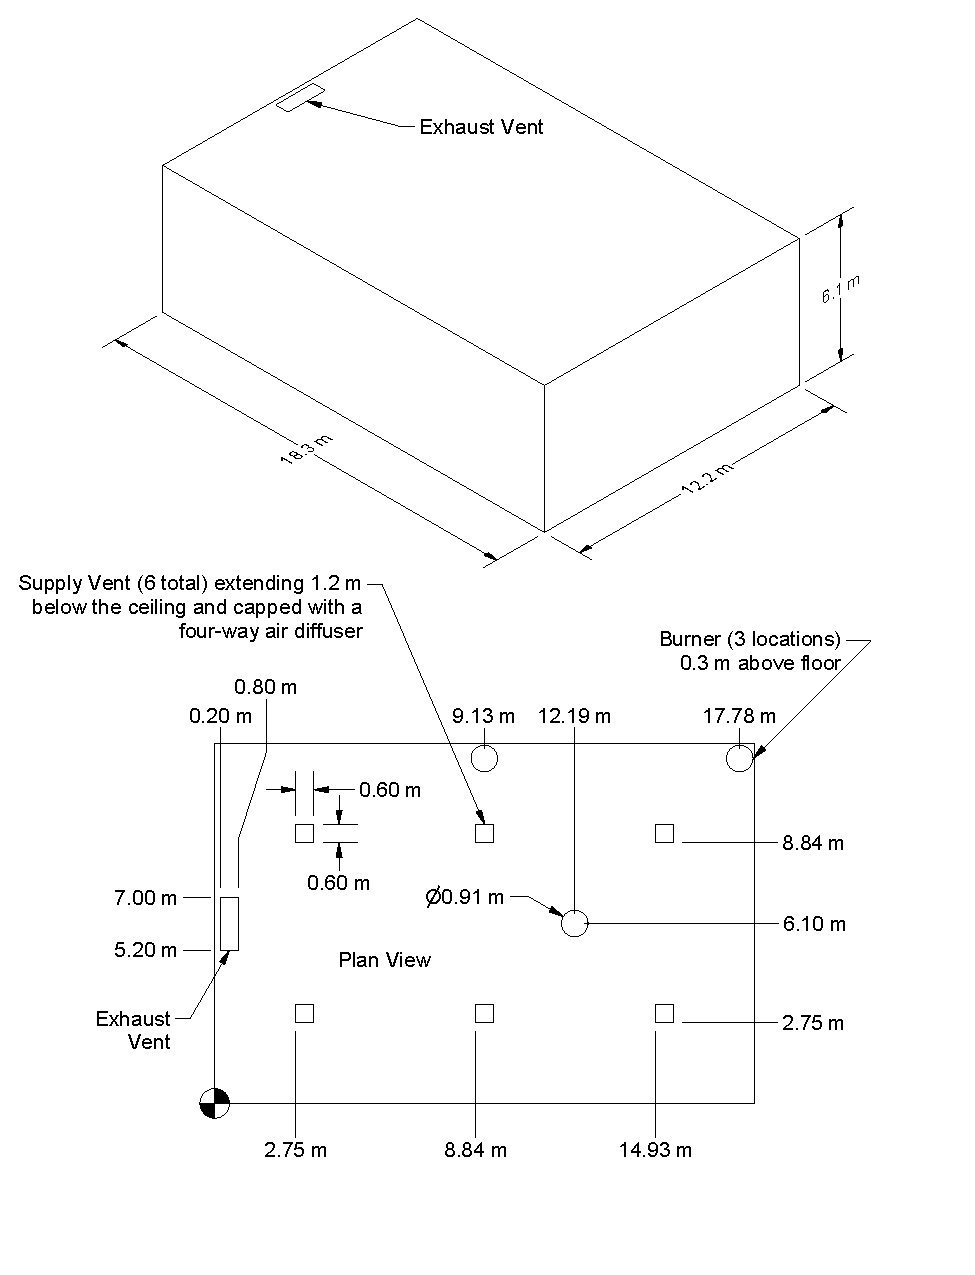
\includegraphics[width=\textwidth]{FIGURES/FM_SNL/FM_SNL_Drawing}
\caption[Geometry of the FM/SNL Experiments]{Geometry of the FM/SNL Experiments.}
\label{FM_SNL_Drawing}
\end{figure}

\FloatBarrier


%\section{FPRF/HAI Corridor Test Series}
%
%The Fire Protection Research Foundation sponsored a series of tests to evalaute the performance of smoke detection mounted in a corridor with deep beam pockets.  The test apparatus consisted of a 14.63 m (48 ft) x 3.66 m (12 ft) movable ceiling to which walls and beams could be attached.  The ceiling was instrumented with gas thermocouples along the centerline,  both at the ceiling and on the bottoms of beams, gas thermocouples along the wall and optical density meters.  21 combinations of beam depth (none, 0.3 m and 0.6 m), corridor width (1.52 m and 3.66 m), and ceiling height (2.74 m, 3.66 m, and 5.49 m) were tested.  Each ceiling height was also tested without walls to serve as an unconfined, smooth ceiling test.  Each test used an 0.3 m (1 ft) x 0.3 m, square sand burner that was centered in the corridor.  Fires were 100 kW propylene fires with a soot yield of 4.8 \% (the soot yield was measured during the test series).  A summary of the tests is shown in Table~\ref{FPRF_HAI_Matrix}.
%
%\begin{table}[h!]
%\caption{Summary of FPRF/HAI Corridor Experiments.}
%\begin{center}
%\begin{tabular}{|c|c|c|c|}
%\hline
%Test    &  Ceiling Height &  Ceiling Width &  Beam Depth  \\
%No.     &  m              &  m             &  m           \\ \hline \hline
%1,2     &  5.49           &  no walls      &  no beams    \\ \hline
%3,4     &  3.66           &  no walls      &  no beams    \\ \hline
%5,6     &  2.74           &  no walls      &  no beams    \\ \hline
%7,8     &  2.74           &  3.66          &  no beams    \\ \hline
%9,10    &  3.66           &  3.66          &  no beams    \\ \hline
%11,12   &  5.49           &  3.66          &  no beams    \\ \hline
%13,14   &  5.49           &  3.66          &  0.30        \\ \hline
%15,16   &  3.66           &  3.66          &  0.30        \\ \hline
%17,18   &  2.77           &  3.66          &  0.30        \\ \hline
%19,20   &  5.49           &  3.66          &  0.61        \\ \hline
%21,22   &  3.66           &  3.66          &  0.61        \\ \hline
%23,24   &  2.74           &  3.66          &  0.61        \\ \hline
%25,26   &  5.49           &  1.52          &  0.61        \\ \hline
%27,28   &  3.66           &  1.52          &  0.61        \\ \hline
%29,30   &  2.74           &  1.52          &  0.61        \\ \hline
%31,32   &  5.49           &  1.52          &  0.30        \\ \hline
%33,34   &  3.66           &  1.52          &  0.30        \\ \hline
%35,36   &  2.74           &  1.52          &  0.30        \\ \hline
%37,38   &  2.74           &  1.52          &  no beams    \\ \hline
%39,40   &  3.66           &  1.52          &  no beams    \\ \hline
%41,42   &  5.49           &  1.52          &  no beams    \\ \hline
%
%\end{tabular}
%\end{center}
%\label{FPRF_HAI_Matrix}
%\end{table}
%
%
%\FloatBarrier

\section{FM Vertical Wall Flame Experiments}
\label{FM_Vertical_Wall_Flame_Description}

A series of experiments was conducted by FM Global~\cite{deRis:IAFSS} in which turbulent flames were generated by flowing various gases through a vertical, water-cooled burner, 1.32~m tall and 0.38~m wide, with 0.152~m side walls. Measurements of soot depth, temperature, radiative heat flux, and radiance were made at various heights.


\section{Frankman Vegetation Experiments}
\label{Frankman_Vegetation_Description}

Experiments were performed by Frankman et al.~\cite{Frankman:CST2010} at Brigham Young University in 2010 in which small wood shavings and pine needles were exposed to various levels of heat flux from a ceramic burner. Small thermocouples recorded the steady state temperatures. The fuel elements were positioned 15~cm, 25~cm, 35~cm, and 45~cm from the 23~cm by 15~cm rectangular ceramic burner with a radiative heat flux of approximately 37~kW/m$^2$. The fuel elements were suspended by a wire with a horizontal orientation. The hydraulic diameters of the small excelsior, large excelsior and Ponderosa pine samples were reported to be 0.44~mm, 1.29~mm, and 0.70~mm, respectively.

\subsubsection{Modeling Notes}

These calculations are performed with a relatively crude grid because typical wildland fire simulations cannot employ fine grids. A free convection correlation for horizontal cylinders is employed for the convective heat transfer coefficient of the fuel samples. Cylindrical Lagrangian particles are used to represent the fuels with diameters equal to the reported hydraulic diameters. The burner is modeled as a hot plate with a radiative heat flux of 37~kW/m$^2$. Nominal values of 0.1~W/m/K, 1~kJ/kg/K, and 450~kg/m$^3$ are assumed for the thermal conductivity, specific heat, and density of the vegetation. The emissivity is assumed to be 1. The results are relatively insensitive to the thermal properties because the final temperatures are largely determined via the balance of radiation heat flux on to and convective heat flux off of the fuel samples. The temperature rise of all samples does not exceed 100~$^\circ$C.


\section{Hamins Gas Burner Experiments}
\label{Hamins_Gas_Burner_Description}

Anthony Hamins of NIST measured the heat flux at various points around gas burner fires~\cite{Hostikka:3}. Three different sized circular burners were used, with diameters of 0.10 m, 0.38 m, and 1.0 m. Three different gases were used, acetylene, methane, and propane. The heat release rates ranged from 2~kW to 200~kW, and values of $\dot{Q}^*$ ranged from 0.04 to 10.6.


\section{Harrison Spill Plumes}
\label{Harrison_Spill_Plumes_Description}

Roger Harrison, a student at the University of Canterbury, New Zealand, performed a series of one-tenth scale experiments to characterize thermal spill plume entrainment~\cite{Harrison:2009,Harrison:IAFSS2008,Harrison:FT2007,Harrison:FSJ2010}. The dimensions of the fire compartment were 1~m by 1~m by 0.5~m high.  The height of the compartment opening was equal to the height of the compartment. The width of the opening was varied from 0.2~m to 1~m.  A 0.3~m balcony was attached to the top of the compartment opening. The balcony extended 0.5~m beyond each side of the fire compartment.  The heat release rate of the fire varied from 5~kW to 15~kW.
The plume entrainment rate was measured at different heights by varying the exhaust rate of gases from a hood above the compartment.
Two different test configurations were used to model both detached and adhered spill plumes. A diagram of the test structure is displayed in Figure~\ref{Harrison_Drawing}.

\begin{figure}[p]
\includegraphics[width=\textwidth]{FIGURES/Harrison_Spill_Plumes/Harrison_Spill_Plumes_Drawing}
\caption{Geometry of the Harrison Spill Plumes Experiments.}
\label{Harrison_Drawing}
\end{figure}




\section{Heskestad Flame Height Correlation}
\label{Heskestad_Flame_Height_Description}

A widely used experimental correlation for flame height is given by the expression~\cite{Heskestad:FSJ1983,SFPE:Heskestad}:
\be
   \frac{L_{\rm f}}{D} = 3.7 \; (\dot{Q}^*)^{2/5} - 1.02  \quad ; \quad \dot{Q}^* = \frac{\dQ}{\rho_\infty \, c_p \, T_\infty \, \sqrt{g} \; D^{5/2} }
\ee
where $\rho_\infty$, $c_p$, and $T_\infty$ are the ambient density, specific heat, and temperature. $\dot{Q}^*$ is a non-dimensional quantity that relates the fire's heat release rate, $\dQ$, with the diameter of its base, $D$. The greater the value of $Q^*$, the higher the flame height relative to its base diameter.

\section{Insulation Material Fire Resistance Tests}
\label{Insulation_Materials_Description}

Paudel et al.~\cite{Paudel:2020} studied small-scale fire resistance tests for 30 different types of stone wool insulation varying in density, thickness, and organic content. During each test, a 60~cm square sample of insulation covered by a 1~mm thick steel plate was mounted to the opening of a small combustion chamber. Thus, one side of the sample was exposed to ambient ($ T_\infty $) conditions, and the other side was attached to the steel plate whose temperature followed the ISO 834 standard fire curve,
\begin{equation}
   T_\textrm{h}(t) = T_\infty + 345 \, \textrm{log}_{10}(8t + 1)
   \label{eq:isocurve}
\end{equation}
with time, $t$, in minutes and exposure temperature, $T_{\textrm{h}}$, in $^\circ$C. The temperature measurements were made using K-type thermocouples covered with 30~mm square inorganic insulating pads. The pads were attached to the back side of the sample using heat-resistant glue or pins.

\subsubsection{Modeling Notes}

The numerical simulation is explained in Ref.~\cite{Paudel:2020}. Because detailed kinetic properties of the material are currently not available, the chemical decomposition parameters ($A$, $E_{\textrm{a}}$ and $n$) were optimized based on the cold-side measured temperatures. Unlike in Ref.~\cite{Paudel:2020}, the optimized values in the simulation are constant, $A=0.0028$~s$^{-1}$, $E_{\textrm{a}}=21700$~J/mol, and $n=0.71$. The optimization used a Monte Carlo method of 1000 Latin hypercube samples, where the sampling range was 0.001 to 1000~s$^{-1}$ for $A$, $1\times10^4$ to $1\times10^5$~J/mol for $E_{\textrm{a}}$, and 0.1 to 1 for $n$.




\section{JH/FRA Rail Car Experiments}
\label{JH_FRA_Description}

Hodges, DiDomizio, Lattimer, and Kapahi~\cite{Hodges:FRA22} conducted a series of seventeen compartment fire tests consisting of fourteen unique configurations and three repeated tests.
Tests were conducted at three scales including full-scale, half-scale, and quarter-scale. 
The baseline full-scale compartment design was based on a standard size National Fire Protection Agency (NFPA) 286 fire room, which is 2.44 m wide, 2.44 m tall, and 3.66 m deep with a single door opening which is 0.9 m wide, and 2.0 m tall.
The initiating fire was a propane burner in the back-left corner of the compartment. 
The reduced-scale compartment designs were geometrically scaled except for the ventilation, which was non-linearly scaled to maintain the equivalence ratio of the compartment. 
The lining material thickness was kept the same at each scalle to preserve the burning duration.

A total of five permutations of the compartment design were evaluated.
The first two scenarios used a specified heat release rate with inert boundaries.
Two heat release rate stages were included in the baseline configuration (non-combustible door configuration), including 5 minutes at a pre-flashover level (full-scale 320 kW) and 5 minutes at a post-flashover level (full-scale 640 kW).
The second scenario, the non-combustible door-window configuration, added a window at the center of the east wall to evaluate the impact of additional ventilation on the scaling approach.
The post-flashover level was increased to ensure flashover with the additional air flow (full-scale 720 kW).

The other scenarios included cases where the heat release rate was dependent on thermal feedback with the fire environment.
Scenarios three and four replaced parts of the inert wall and ceiling material in the non-combustible door configuration with combustible linings.
Two different combustible materials were used: plywood and a fiber-reinforced plastic (FRP).
The last scenario used a kerosene-type jet fuel, JP-5, in the same geometric configuration as the non-combustible door configuration but replaced the propane burner with a liquid pool fire.

Table \ref{JH_FRA_Matrix} provides a summary of the experiments. 
Each HRR listed for cases with non-combustible lining (NC) corresponded to a separate 5-minute exposure level (i.e., test 2 had 3 stages each 5 minutes long starting at 20 kW, then increasing the burner to 45 kW, then a final 5-minute stage at 50 kW).

\begin{table}[!htb]
\caption[Summary of JH/FRA Rail Car Experiments]{Summary of JH/FRA Rail Car Experiments.~\cite{Hodges:FRA22}}
\begin{center}
\begin{tabular}{|c|c|c|c|c|c|c|}
\hline
Test & Scale   & Lining   &  Initiating & Peak       & Ventilation   & Fuel Type \\
No.  & Config. & Material &  HRR (kW)   & HRR (kW)   &               &           \\ \hline \hline
1    & Quarter & NC       & 20/40       & 20/40      & Door          & Propane   \\ \hline
2    & Quarter & NC       & 20/45/50    & 20/45/50   & Door + Window & Propane   \\ \hline
3    & Quarter & Plywood  & 40          & 113        & Door          & Propane   \\ \hline
4    & Quarter & FRP      & 40          & 87         & Door          & Propane   \\ \hline
5    & Quarter & NC       & -           & 60         & Door          & JP-5      \\ \hline
6    & Half    & NC       & 80/160      & 80/160     & Door          & Propane   \\ \hline
7    & Half    & NC       & 80/160/200  & 80/160/200 & Door + Window & Propane   \\ \hline
8    & Half    & Plywood  & 160         & 466        & Door          & Propane   \\ \hline
9    & Half    & FRP      & 160         & 400        & Door          & Propane   \\ \hline
10   & Half    & NC       & -           & 110        & Door          & JP-5      \\ \hline
11   & Full    & NC       & 720/1,430   & 720/1,430  & Door          & Propane   \\ \hline
12   & Full    & NC       & 720/1,610   & 720/1,610  & Door + Window & Propane   \\ \hline
13   & Full    & Plywood  & 1,430       & 5,500      & Door          & Propane   \\ \hline
14   & Full    & FRP      & 1,430       & 4,500      & Door          & Propane   \\ \hline

\end{tabular}
\end{center}
\label{JH_FRA_Matrix}
\end{table}

The instrumentation plan from the test series is shown in Figure ~\ref{JH_FRA_instrumentation_fig}. 
Dimensions for each scale are summarized in Tables \ref{JH_FRA_instrumentation_tab1}-\ref{JH_FRA_instrumentation_tab4}.

\begin{figure}[h!]
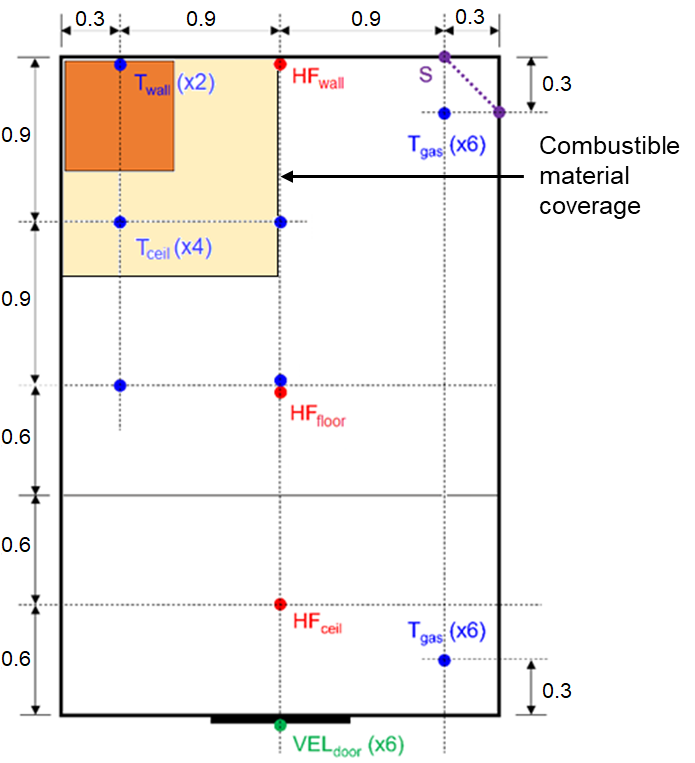
\includegraphics[width=0.49\textwidth]{FIGURES/JH_FRA/JH_FRA_instrumentation1}
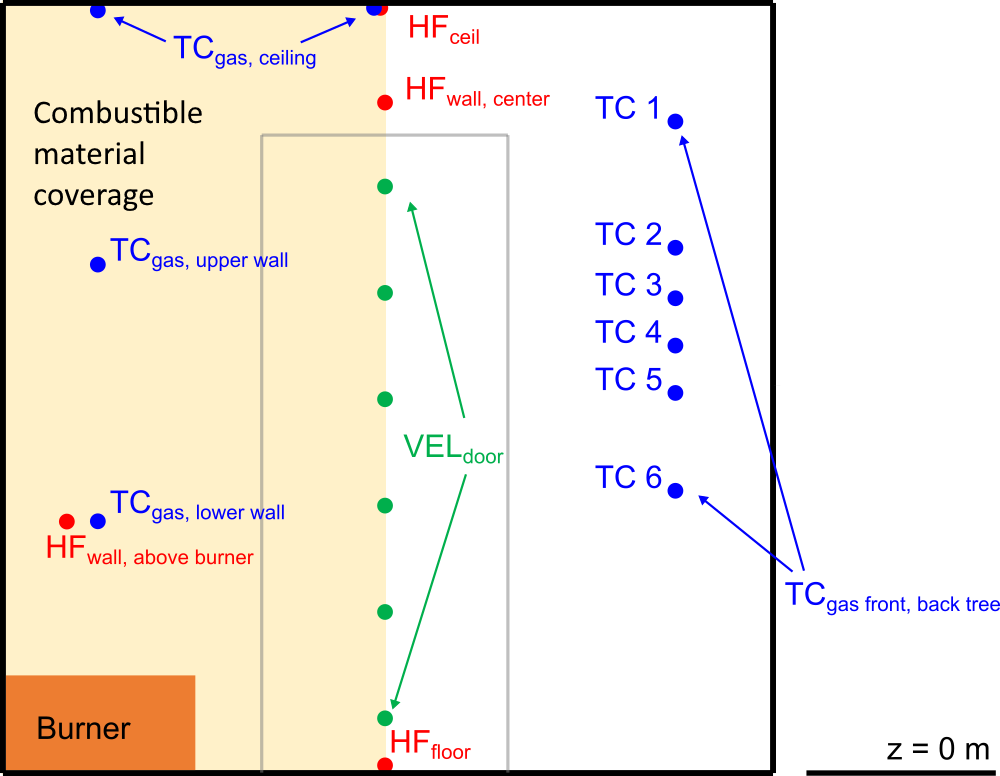
\includegraphics[width=0.49\textwidth]{FIGURES/JH_FRA/JH_FRA_instrumentation2} \\
\caption[Instrumentation plan from compartment fire experiments]{Instrumentation plan from compartment fire experiments (left) plan view (right) front view).}
\label{JH_FRA_instrumentation_fig}
\end{figure}

\begin{table}[h!]
\begin{center}
\caption[Dimensions for instrumentation schematic]{Dimensions for instrumentation schematic~\cite{Hodges:FRA22}.} \label{JH_FRA_instrumentation_tab1}
\begin{tabular}{|l|c|c|c|c|c|} \hline
Scale   & \si{W_1}     & \si{W_2}     & \si{H_1}     & \si{H_2}    & \si{H_3}  \\
        & \si{\m}      & \si{\m}      & \si{\m}      & \si{\m}     & \si{\m}   \\
\hline \hline
Full    & 0.30  &  0.91   & 0.91    & 0.61   & 0.30    \\ \hline
Half    & 0.15  &  0.46   & 0.46    & 0.30   & 0.15    \\ \hline
Quarter & 0.08  &  0.23   & 0.23    & 0.15   & 0.08    \\ \hline
\end{tabular}
\end{center}
\end{table}

\begin{table}[h!]
\begin{center}
\caption[Thermocouple tree heights]{Thermocouple tree heights~\cite{Hodges:FRA22}.} \label{JH_FRA_instrumentation_tab2}
\begin{tabular}{|l|c|c|c|c|c|c|} \hline
Scale   & \si{TC 1}     & \si{TC 2}     & \si{TC 3}     & \si{TC 4}    & \si{TC 5}   & \si{TC 6}   \\
        & \si{\m}       & \si{\m}       & \si{\m}       & \si{\m}      & \si{\m}     & \si{\m}     \\
\hline \hline
Full    & 2.08  &  1.68   & 1.52    & 1.37   & 1.22   & 0.91   \\ \hline
Half    & 1.04  &  0.84   & 0.76    & 0.69   & 0.61   & 0.46   \\ \hline
Quarter & 0.52  &  0.42   & 0.38    & 0.34   & 0.30   & 0.23   \\ \hline
\end{tabular}
\end{center}
\end{table}

\begin{table}[h!]
\begin{center}
\caption[Ventilation velocity heights]{Ventilation velocity heights~\cite{Hodges:FRA22}.} \label{JH_FRA_instrumentation_tab3}
\begin{tabular}{|l|c|c|c|c|c|c|c|c|} \hline
Scale   & \si{Door 1}     & \si{Door 2}     & \si{Door 3}     & \si{Door 4}    & \si{Door 5}   & \si{Door 6}  & \si{Window 1}    & \si{Window 2}   \\
        & \si{\m}       & \si{\m}       & \si{\m}       & \si{\m}      & \si{\m}     & \si{\m}      & \si{\m}    & \si{\m} \\
\hline \hline
Full    & 0.168 &  0.505   & 0.842  & 1.179   & 1.516   & 1.853   & 1.372    & 1.525 \\ \hline
Half    & 0.084 &  0.253   & 0.421  & 0.590   & 0.758   & 0.927   & 0.686    & 0.762 \\ \hline
Quarter & 0.042 &  0.126   & 0.211  & 0.295   & 0.379   & 0.463   & 0.343    & 0.381 \\ \hline
\end{tabular}
\end{center}
\end{table}

\begin{table}[h!]
\begin{center}
\caption[Heat flux heights]{Heat flux heights~\cite{Hodges:FRA22}.} \label{JH_FRA_instrumentation_tab4}
\begin{tabular}{|l|c|c|c|c|} \hline
Scale   & \si{Ceiling}     & \si{Wall}     & \si{Burner}     & \si{Floor}   \\
        & \si{\m}       & \si{\m}       & \si{\m}       & \si{\m}    \\
\hline \hline
Full    & 2.44 &  1.83   & 0.813  & 0.000 \\ \hline
Half    & 1.22 &  0.92   & 0.407  & 0.000 \\ \hline
Quarter & 0.61 &  0.46   & 0.203  & 0.000 \\ \hline
\end{tabular}
\end{center}
\end{table}

\FloatBarrier

\subsubsection{Modeling Notes}

The combustible lining experiments in this study are used to evaluate a scaling-based simplified pyrolysis model.
The model input parameters used in simulating these experiments are summarized in Table \ref{JH_FRA_Properties}.
Additional detail on these properties can be found in previous test reports~\cite{Luo:FRA2019,Lattimer:NIJ19}.
The cone calorimeter data used as a reference for the scaling-based pyrolysis model is the 50 \si{kW/m^2} curve provided in Figure \ref{JH_FRA_plywood_cone}.

\begin{table}[h!]
\begin{center}
\caption[Parameters for JH/FRA simulations]{Parameters for JH/FRA simulations~\cite{Hodges:FRA22}.} \label{JH_FRA_Properties}
\begin{tabular}{|l|c|c|c|c|c|} \hline
        & $\rho$               & $c_p$                        & $k$                & $T_{ign}$       & $\Delta$  \\
Fuel    & \si{\kg/\m^3}        & \si{\kJ/(\kg.\K)}            & \si{\W/(\m.\K)}    & \si{^{$\circ$}}C   & \si{mm} \\
\hline \hline
Plywood  &  625  &  3.13   & 0.295  & 287  & 7.2     \\ \hline
FRP      &       &         &        &      &         \\ \hline
\end{tabular}
\end{center}
\end{table}

\begin{figure}[p]
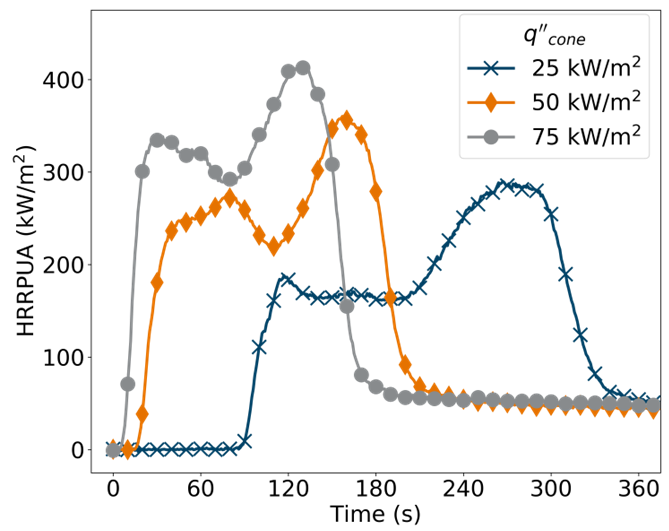
\includegraphics[width=\textwidth]{FIGURES/JH_FRA/JH_FRA_plywood_cone}
\caption[Plywood heat release rate per unit area]{Plywood heat release rate per unit area.}
\label{JH_FRA_plywood_cone}
\end{figure}

\FloatBarrier






\section{LEMTA Spray Test for Radiation Attenuation}
\label{LEMTA_Spray_Description}

Lechene et al.~\cite{Lechene} measured the attenuation of thermal radiation passing through a water spray using a heat flux gauge. The radiation was produced by a 30~cm by 35~cm heat panel whose emission was close to a black body at 500~$^\circ$C. The horizontal distance from the radiation panel to the spray nozzle was 1.5~m and to the measurement point 3~m. The heat flux gauge was positioned at the line passing through the center of the panel. Seven nozzles were arranged in a row, 10~cm apart. They were positioned 1.5~m high. The heat panel was translated vertically during the experiment, the distance between the panel upper edge and the nozzle row varying between 20~cm and 100~cm. The attenuation of radiation is defined as previously described for the BRE Spray experiments. The purpose of the simulations is to compare the measured and simulated attenuation of radiation at different heights. The water mist nozzle has been characterized by Lechene by measuring the spray angles and the water flow rate. The droplet size is set by using a PDPA measurement in a single position, 20~cm below the injection point.


\section{LLNL Enclosure Experiments}
\label{LLNL_Enclosure_Description}

Sixty-four compartment experiments were conducted at Lawrence Livermore National Laboratory (LLNL) in 1986 to study the effects of ventilation on enclosure fires~\cite{Foote:LLNL1986}. These experiments are the basis of the Foote, Pagni, Alvares compartment temperature correlation~\cite{Foote:IAFSS1}.

The test enclosure was 6~m long, 4~m wide, and 4.5~m high (Fig.~\ref{LLNL_Enclosure_Drawing}) with a methane rock burner in the center of the space positioned at various elevations. For most of the experiments the burner was placed on the floor. The fires varied in size, $\dot{Q}$, from 50~kW to 400~kW. The burner was 0.57~m in diameter and 0.23~m height. A single door was closed and sealed for most experiments, and air was pulled through the compartment at rates, $\dot{m}$, varying from 100~g/s to 500~g/s. In some tests the enclosure included a plenum space, where make-up air could be injected from above or below. The test matrix is listed in Table~\ref{LLNL_Matrix}.

\begin{table}[p]
\caption[Summary of LLNL Enclosure Experiments]{Summary of LLNL Enclosure Experiments.}
\begin{center}
\begin{tabular}{|c|c|c|c|c|c|c||c|c|c|c|c|c|c|}
\hline
Test & Room    & $h_0$ &  $\dot{Q}$ & $\dot{m}$ & $T_\infty$ & $t_{\rm end}$  &   Test & Room    & $h_0$ &  $\dot{Q}$ & $\dot{m}$ & $T_\infty$ & $t_{\rm end}$  \\
No.  & Config. & m     &  kW        & g/s       & $^\circ$C  & s              &   No.  & Config. & m     &  kW        & g/s       & $^\circ$C  & s           \\ \hline \hline
1    & TL      & 0     & 200        & 0         & 23         & 560            &   33   & PH      & 0     & 100        & 200       & 23         & 5100        \\ \hline
2    & TL      & 0     & 200        & 0         & 27         & 545            &   34   & PH      & 0     & 100        & 300       & 34         & 4280        \\ \hline
3    & TL      & 0     & 400        & 0         & 27         & 300            &   35   & PH      & 0     & 100        & 400       & 22         & 4110        \\ \hline
4    & TL      & 0     & 300        & 0         & 24         & 385            &   36   & PH      & 0     & 100        & 500       & 29         & 4060        \\ \hline
5    & TL      & 0     & 50         & 0         & 28         & 2770           &   37   & PH      & 0     & 200        & 100       & 20         & 520         \\ \hline
6    & TL      & 0     & 100        & 0         & 29         & 1295           &   38   & PH      & 0     & 200        & 300       & 29         & 4100        \\ \hline
7    & TL      & 0     & 100        & 0         & 35         & 1240           &   39   & PH      & 0     & 250        & 100       & 18         & 430         \\ \hline
8    & TL      & 0     & 200        & 0         & 35         & 555            &   40   & PH      & 0     & 200        & 400       & 28         & 4290        \\ \hline
9    & TL      & 0     & 200        & 500       & 33         & 4220           &   41   & PH      & 0     & 150        & 100       & 20         & 970         \\ \hline
10   & TL      & 0     & 200        & 100       & 28         & 6050           &   42   & PHE     & 2     & 200        & 180       & 30         & 5120        \\ \hline
11   & TL      & 0     & 200        & 200       & 18         & 4780           &   43   & PHE     & 2     & 200        & 0         & 32         & 570         \\ \hline
12   & TL      & 0     & 200        & 300       & 21         & 5440           &   44   & PHE     & 1     & 200        & 180       & 19         & 2670        \\ \hline
13   & TL      & 0     & 200        & 400       & 28         & 5150           &   45   & PHE     & 1     & 200        & 0         & 30         & 810         \\ \hline
14   & TL      & 0     & 200        & 400       & 28         & 5090           &   46   & PHE     & 0.6   & 200        & 180       & 19         & 960         \\ \hline
15   & TL      & 0     & 100        & 300       & 24         & 4070           &   47   & PHE     & 0.6   & 200        & 0         & 19         & 730         \\ \hline
16   & TL      & 0     & 200        & 300       & 21         & 6560+          &   48   & PHE     & 0.3   & 200        & 0         & 21         & 520         \\ \hline
17   & PL      & 0     & 200        & 500       & 26         & 3980           &   49   & PHE     & 0.3   & 200        & 180       & 26         & 970         \\ \hline
18   & PL      & 0     & 200        & 400       & 21         & 4840           &   50   & PHE     & 1     & 200        & 180       & 21         & 4730        \\ \hline
19   & PL      & 0     & 200        & 300       & 18         & 5110           &   51   & PNE     & 1     & 200        & NAT       & 33         & 3360        \\ \hline
20   & PL      & 0     & 200        & 200       & 16         & 6570           &   52   & PN      & 0     & 200        & NAT       & 23         & 4680        \\ \hline
21   & PL      & 0     & 200        & 100       & 23         & 6570           &   53   & PHGS    & 0     & 200        & 185       & 33         & 1540        \\ \hline
22   & PH      & 0     & 200        & 190       & 30         & 950            &   54   & PHGS    & 0     & 200        & 215       & 21         & 4180        \\ \hline
23   & PH      & 0     & 200        & 215       & 28         & 4260           &   55   & PN      & 0     & 100        & NAT       & 31         & 4120        \\ \hline
24   & PH      & 0     & 200        & 205       & 26         & 1480           &   56   & PHGW    & 0     & 200        & 190       & 20         & 1240        \\ \hline
25   & PH      & 0     & 200        & 205       & 25         & 2050           &   57   & PHGW    & 0     & 200        & 215       & 29         & 5390        \\ \hline
26   & PH      & 0     & 200        & 500       & 24         & 4100           &   58   & PHX     & 0     & 200        & 190       & 18         & 4090        \\ \hline
27   & PH      & 0     & 200        & 100       & 23         & 540            &   59   & PHXE    & 1     & 200        & 190       & 24         & 4090        \\ \hline
28   & PH      & 0     & 150        & 150       & 31         & 1870           &   60   & PN      & 0     & 400        & NAT       & 22         & 2680        \\ \hline
29   & PH      & 0     & 250        & 250       & 28         & 1520           &   61   & TN      & 0     & 200        & NAT       & 31         & 2730        \\ \hline
30   & PH      & 0     & 250        & 300       & 34         & 4080           &   62   & TN      & 0     & 400        & NAT       & 22         & 2660        \\ \hline
31   & PH      & 0     & 250        & 500       & 36         & 4160           &   63   & TN      & 0     & 50         & NAT       & 28         & 3240        \\ \hline
32   & PH      & 0     & 100        & 100       & 33         & 4110           &   64   & TN      & 0     & 100        & NAT       & 17         & 3570        \\ \hline
\end{tabular}
\end{center}
\begin{tabbing}
\hspace{0.7in} \= T \hspace{0.2in}  \= full compartment     \hspace{0.8in} \= N \hspace{0.2in} \= natural ventilation (door open) \\
               \> P                 \> plenum configuration                \> X                \> 3 ft extension on inlet opening \\
               \> L                 \> low inlet duct                      \> GS               \> grate on inlet, north/south configuration \\
               \> H                 \> high inlet duct                     \> GW               \> grate on inlet, east/west configuration \\
               \> E                 \> elevated fire, $h_0$
\end{tabbing}
\label{LLNL_Matrix}
\end{table}

\begin{figure}[p]
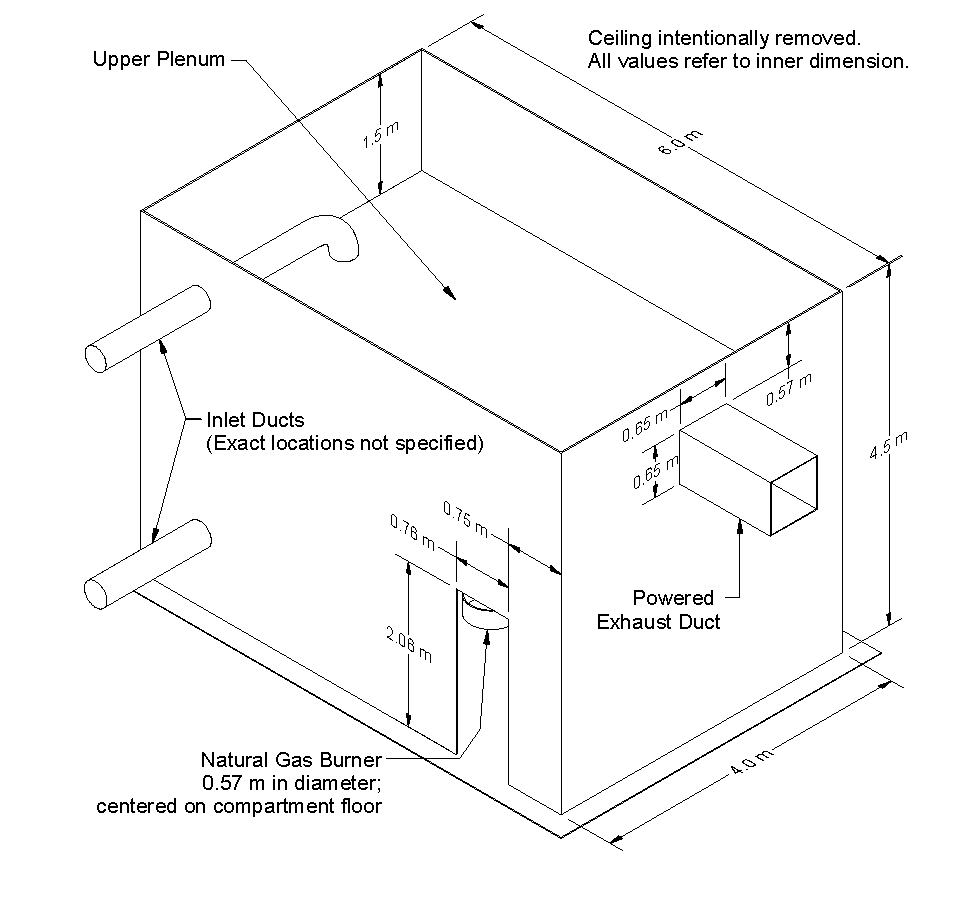
\includegraphics[width=\textwidth]{FIGURES/LLNL_Enclosure/LLNL_Enclosure_Drawing}
\caption[Geometry of the LLNL Enclosure Experiments]{Geometry of the LLNL Enclosure Experiments.}
\label{LLNL_Enclosure_Drawing}
\end{figure}

\subsubsection{Modeling Notes}

The LLNL Enclosure is modeled using a single mesh spanning the interior of the test compartment. The heat release rate of the methane burner and the thermal properties of the walls, ceiling and floor are specified based on information provided in the test report.

The test report of the LLNL Enclosure experiments lists the mass flow rate, $\dot{m}$, through the exhaust duct during the experiment. This mass flow rate is specified explicitly in the model. The make-up air into the compartment is supplied by an inlet duct and compartment leakage, both of which are modeled. The inlet duct is modeled as a 7~m long, 30~cm diameter circular duct with a loss coefficient of 25.6. The leakage area is then calculated based on the reported compartment under or over-pressures, $\Delta p$, during the experiment. The leak area is computed based on the following formulae:
\be
   \frac{\dot{m}}{\rho} = A_{\rm L} \, \sqrt{\frac{2 \, |\Delta p|}{\rho}}  \quad ; \quad A_{\rm L} = A_{\rm L,ref} \left( \frac{|\Delta p|}{|\Delta p_{\rm ref}|} \right)^{n-0.5}
\ee
The reference leakage area, $A_{\rm L,ref}$, is estimated to be 0.0033~m$^2$, $n=0.6311$, $\Delta p_{\rm ref}=50$~Pa.

In some of the experiments, the fire was reported to have self-extinguished, in which case the model employs the relatively simple Mowrer extinction model along with the one-step fast chemistry model of combustion. The Mowrer model predicts local flame extinction when the oxygen concentration within a grid cell is less than that required to raise the cell temperature to the critical flame temperature, which is 1507~$^\circ$C for methane~\cite{SFPE:Beyler}.


\section{LNG Dispersion Experiments}
\label{LNG_Dispersion_Description}

In 2006, the Fire Protection Research Foundation (FPRF) undertook a research project for the National Fire Protection Association (NFPA) Liquefied Natural Gas (LNG) Technical Committee to develop tools for evaluating LNG dispersion models. The work was carried out by the Health and Safety Laboratory (HSL), a directorate of the UK Health and Safety Executive (HSE). HSL developed the LNG Model Evaluation Protocol (MEP), which contained a structure for complete evaluation of LNG dispersion models~\cite{Ivings:HSL}. The experiments are described in Ref.~\cite{Stewart:HSL}.

\subsubsection{Modeling Notes}

The simulations of liquefied natural gas (LNG) dispersion experiments that are described in this report were originally designed by Jeffrey Engerer and Anay Luketa of Sandia National Laboratories on behalf of the Pipeline and Hazardous Materials Safety Administration of the U.S. Department of Transportation.

Parameters for the LNG dispersion experiments are given in Table~\ref{tab:LNG_Dispersion}. In some cases, values of the Monin-Obukhov parameters are taken directly from the test reports. However, for some of the experiments, these parameters were not derived using the same similarity functions as those presented above, in which case the parameters have been recomputed to best fit the measured velocity and temperature profiles. In the table, $u_*$ is the friction velocity, $\kappa=0.41$ is the Von K\'{a}rm\'{a}n constant, $z_0$ is the \emph{aerodynamic} roughness length, $\theta_*$ is the scaling potential temperature, $\theta_0$ is the ground level potential temperature, $L$ is the Monin-Obukhov length, and the similarity functions are those proposed by Dyer~\cite{Dyer:1974} and discussed in the report of the Falcon field experiments~\cite{Falcon}.

In the experiments, a fixed mass, $m$, of LNG was spilled onto water, forming a pool of increasing radius. For modeling purposes, it is assumed that the mass flux of natural gas from the circular pool is fixed at $\dot{m}''_{\rm max}=0.167$~kg/(m$^2 \cdot$s), and the temperature of the gas is $-162$~$^\circ$C, as suggested in the testing protocols. The diameter of the pool, $D$, is calculated using the assumed mass flux per unit area, the reported mass of LNG, $m$, and the spill duration, $\Delta t$.
\be
   D = \sqrt{ \frac{4 \, m}{\pi \, \dot{m}''_{\rm max} \, \Delta t} }
\ee
The values of $D$ are given in Table~\ref{tab:LNG_Dispersion}.

\begin{sidewaystable}[p]
\caption[Summary of LNG Dispersion Experiments]{Summary of LNG Dispersion Experiments.}
\begin{center}
\begin{tabular}{|l|c|c|c|c|c|c|c|c|c|c|c|c|c|}
\hline
Series                         & \multicolumn{4}{|c|}{Burro}       & \multicolumn{3}{|c|}{Coyote}  & \multicolumn{3}{|c|}{Falcon}                  & \multicolumn{3}{|c|}{Maplin Sands}          \\ \hline
Number                         & 3      & 7      & 8      & 9      &  3     & 5      & 6           &  1          & 3           & 4                 &  27             & 34             & 35      \\ \hline \hline
\multicolumn{14}{|c|}{Parameters supplied by test reports} \\ \hline
Fuel Mass, $m$ (kg)            & 14712  & 17289  & 12453  & 10730  & 6532   & 12676  & 10139       & 28074       & 21435       & 18984             & 3714            & 2094           & 3658    \\ \hline
Spill Duration, $\Delta t$ (s) & 167    & 174    & 107    & 79     & 65     & 98     & 82          & 131         & 154         & 301               & 160             & 95             & 135     \\ \hline
$p_0$ (mbar)                   & 948    & 940    & 941    & 940    & 936    & 939    & 942         & 908.9       & 900.8       & 906.3             & ---             & ---            & ---     \\ \hline
$T_0$ ($^\circ$C)              & 34.5   & 33.8   & 32.9   & 35.4   & 39.6   & 29.3   & 24.1        & 32.2        & 35.0        & 30.8              & 14.9            & 15.2           & 16.1    \\ \hline
RH (\%)                        & 5.2    & 7.4    & 4.5    & 14.4   & 11.3   & 22.1   & 22.8        & ---         & 4.0         & 12.0              & 53              & 90             & 77      \\ \hline
\multicolumn{14}{|c|}{Computed parameters} \\ \hline
$L$ (m)                        & -9.49  & -111   & 16.2   & -142   & -8.56  & -33.2  & 82.5        & 4.96        & -422        & 69.4              & -14.4           & -75.5          & -81.2   \\ \hline
$u_*$ (m/s)                    & 0.255  & 0.372  & 0.074  & 0.252  & 0.310  & 0.480  & 0.210       & 0.061       & 0.305       & 0.369             & 0.190           & 0.280          & 0.315   \\ \hline
$z_0$ (m)                      & 0.0002 & 0.0002 & 0.0002 & 0.0002 & 0.0002 & 0.0002 & 0.0002      & 0.008       & 0.008       & 0.008             & 0.0003$^\ddag$  & 0.0003$^\ddag$ & 0.0003$^\ddag$  \\ \hline
$\theta_*$ (K)                 & -0.532 & -0.097 & 0.026  & -0.035 & -0.890 & -0.520 & 0.039       & 0.058       & -0.018      & 0.152             & -0.180          & -0.075         & -0.088  \\ \hline
$\dot{q}''$ (W/m$^2$)          & -154   & -41    & 2      & -10    & -314   & -284   & 9           & 4           & -5          & 58                & -39             & -24            & -32     \\ \hline
$D$ (m)                        & 25.9   & 27.5   & 29.9   & 32.2   & 27.7   & 31.4   & 30.6        & 19.5$^\dag$ & 16.0$^\dag$ & 10.8$^\dag$       & 13.3            & 12.8           & 14.4    \\ \hline
\end{tabular}
\end{center}
$^\ddag$ The roughness length was changed to 0.00002~m to better match the measured velocity and temperature profiles

$^\dag$ The Falcon experiments involved 4 separated spills
\label{tab:LNG_Dispersion}
\end{sidewaystable}



\section{Loughborough Jet Fire Experiments}
\label{Loughborough_Jet_Fires_Description}

Researchers at Loughborough University, UK, conducted a series of six large-scale, high pressure jet fire experiments using natural gas and natural gas/hydrogen mixtures at the GL Noble Denton Spadeadam Test Site in Cumbria, UK~\cite{Lowesmith:PSEP2012}. For each fuel, the gas was released horizontally at high pressure (approximately 60~bar) through 20~mm, 35~mm and 50~mm diameter holes at the end of a 15~cm diameter pipe. The jet fires engulfed a 0.9~m diameter, 16~m long pipe section perpendicular to the flow direction. Heat flux measurements were made at various locations on the pipe and further afield. A typical jet fire experiment at the facility is shown in Fig.~\ref{jet_photo}.

\begin{figure}[!ht]
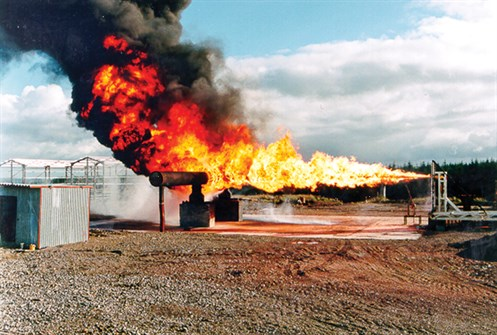
\includegraphics[width=\textwidth]{FIGURES/Loughborough_Jet_Fires/Safety-Fig-03_497x335}
\caption[Photograph of a jet fire experiment at the Spadeadam Test Site]{Photograph of a jet fire experiment at the Spadeadam Test Site.}
\label{jet_photo}
\end{figure}

Table~\ref{Loughborough_Parameters} lists the key parameters for the natural gas experiments which have been chosen for this study. Note that the direction of the jet was nominally to the east, parallel to the prevailing wind. The wind deviated slightly in each experiment, as indicated in the table.

\begin{table}[!ht]
\caption[Summary of the Loughborough Jet Fire Experiments]{Summary of the Loughborough Jet Fire Experiments.}
\begin{tabular}{|c|c|c|c|c|c|c|c|c|c|c|}
\hline
Test    & Fuel     & Hole  & Dist.    & Wind          & Wind    & Mass   & Heat Rel.    & Flame     & Stand-Off  & Rad.      \\
No.     & Type     & Diam. & to Pipe  & Dir.          & Speed   & Flow   & Rate         & Length    & Distance   & Frac.     \\ 
        &          & (mm)  & (m)      & ($^\circ$)    & (m/s)   & (kg/s) & (MW)         & (m)       & (m)        & (\%)      \\ \hline
1       & Nat.~Gas & 20    & 9.45     & 271           & 6.3     & 2.9    & 140          & 19.8      & 6.0        & 13.7      \\
2       & Nat.~Gas & 35    & 15.45    & 297           & 6.2     & 9.6    & 462          & 37.8      & 7.5        & 17.9      \\
3       & Nat.~Gas & 50    & 21.61    & 267           & 3.6     & 19.5   & 939          & 49.9      & 8.7        & 20.2      \\ \hline
\end{tabular}
\label{Loughborough_Parameters}
\end{table}

\subsubsection{Modeling Notes}

FDS is a low Mach number code and cannot model directly the supersonic flow at the pipe orifice. Instead, cold (-160~$^\circ$C) droplets with a median volumetric diameter of 1000~$\mu$m are injected wtih an initial velocity of 1000~m/s and spray angle of 10$^\circ$. These droplets evaporate readily to form methane gas. No attempt is made to model the stand-off distance because there is no mechanism in FDS to account for flame suppression due to high shear.

The grid resolution is 20~cm; thus, the circular pipe is modeled as a collection of 20~cm square rods with a cross section that is 0.8~m by 0.8~m, but with the corners removed. The velocity boundary condition is assumed to be free-slip because otherwise the polygonally-shaped obstruction would exert a fictitiously high drag force on the flow. The empirical heat transfer coefficient for the pipe is calculated using parameters appropriate for a cylindrical rather than a flat plate. The Nusselt number is taken as 
\be
   \NU = 0.027 \, \RE^{0.805} \, \PR^{1/3} \quad ; \quad \RE = \frac{\rho D \|\bu_{\rm t}\| }{\mu} \quad ; \quad \PR=0.7
\ee
This correlation is appropriate for $40,000 < \RE < 400,000$~\cite{Incropera:1}.

The values of radiative fraction in the model are based on the measured values reported in Table~\ref{Loughborough_Parameters}. To resolve the radiation field at the far-field radiometers, 600~angles are used in solving the radiation transport equation rather than the default 100. The radiation absorption coefficients are calculated by RadCal assuming a path length of 100~m rather than the default value of 0.1~m. 

The wind profile is based on measurements made 10.85~m above the relatively flat terrain. The aerodynamic roughness length, $z_0$, is set to 0.03~m, appropriate for relatively flat grasslands, prairies, farms, etc. The Obukhov length, $L$, is set to 100,000~m, typical of a neutral atmosphere. Synthetic turbulence is generated at the upstream boundary of the computational domain, with a characteristic eddy length scale of 1~m and root-mean-square velocity fluctuation of 0.1~m/s.

\begin{description}
\item[Flame Length Results:] Section~\ref{Flame Height}
\item[Heat Flux Results:] Section~\ref{Loughborough_Jet_Fires_Heat_Flux}
\end{description}


\FloatBarrier


\section{McCaffrey Plume Experiments}
\label{McCaffrey_Plume_Description}

In 1979, at the National Bureau of Standards (now NIST), Bernard McCaffrey measured centerline temperature and velocity profiles above a porous, refractory burner. There were five distinct heat release rates, ranging from 14~kW to 57~kW. The fuel was natural gas (35 kJ/L [45 MJ/kg assuming 19 kg/kgmol as mole weight for natural gas]). The burner was square, 0.3~m on each side. The results of the experiments are reported in Reference~\cite{McCaffrey:NBSIR_79-1910}. Along the centerline of the burner, velocity and temperature were measured using bi-directional probes and thermocouples, respectively.  The centerline data collapses when scaled by the Froude number as shown in Fig.~\ref{fig:McCaffrey_Correlations}. Radiant fraction measurements for natural gas were made in \cite{McCaffrey:1981}.  For convenience, we have extracted the data from that report for the heat release rates reported in \cite{McCaffrey:NBSIR_79-1910}.  See Table \ref{tab:McCaffrey_Plume_Exp}.  The burner surface temperatures are extrapolated to the surface location from a least squares fit of of the temperature data below $z/Q^{2/5} = 0.05$ \si{m.kW^{-2/5}}.  The extrapolations for each power are shown in Fig.~\ref{fig:McCaffrey_Surf_Temp}.

\begin{figure}[!ht]
\begin{tabular*}{\textwidth}{l@{\extracolsep{\fill}}r}
\includegraphics[height=2.2in]{SCRIPT_FIGURES/McCaffrey_Plume/McCaffrey_Temperature_Correlation} &
\includegraphics[height=2.2in]{SCRIPT_FIGURES/McCaffrey_Plume/McCaffrey_Velocity_Correlation} \\
\end{tabular*}
\caption[McCaffrey Plume Centerline Temperature and Velocity Correlations]
{McCaffrey Plume Centerline Temperature and Velocity Correlations (dashed lines) and raw data (symbols).}
\label{fig:McCaffrey_Correlations}
\end{figure}

\begin{table}[!ht]
\caption[Summary of McCaffrey Plume Experiments]{Summary of McCaffrey Plume Experiments, 1979.}
\begin{center}
\begin{tabular}{|c|c|c|c|c|c|}
\hline
$Q$ (kW) & $Q^*$    & $D^*$ (m)   & HRRPUA (kW/m$^2$)  & $\chi_r$ & $T_{\rm surf}$ (\si{\degreeCelsius}) \\ \hline\hline
14.4     & 0.270    & 0.178       & 160                & 0.17     & 750 \\ \hline
21.7     & 0.407    & 0.209       & 241                & 0.21     & 716 \\ \hline
33.0     & 0.618    & 0.248       & 367                & 0.25     & 630 \\ \hline
44.9     & 0.841    & 0.280       & 499                & 0.27     & 608 \\ \hline
57.5     & 1.07     & 0.309       & 639                & 0.27     & 534 \\ \hline
\end{tabular}
\end{center}
\label{tab:McCaffrey_Plume_Exp}
\end{table}

\begin{figure}[p]
\begin{tabular*}{\textwidth}{l@{\extracolsep{\fill}}r}
\includegraphics[height=2.2in]{SCRIPT_FIGURES/McCaffrey_Plume/McCaffrey_14kW_Surface_Temp} &
\includegraphics[height=2.2in]{SCRIPT_FIGURES/McCaffrey_Plume/McCaffrey_22kW_Surface_Temp} \\
\includegraphics[height=2.2in]{SCRIPT_FIGURES/McCaffrey_Plume/McCaffrey_33kW_Surface_Temp} &
\includegraphics[height=2.2in]{SCRIPT_FIGURES/McCaffrey_Plume/McCaffrey_45kW_Surface_Temp} \\
\includegraphics[height=2.2in]{SCRIPT_FIGURES/McCaffrey_Plume/McCaffrey_57kW_Surface_Temp} &
\end{tabular*}
\caption[McCaffrey Plume Burner Surface Temperatures]
{McCaffrey Plume Burner Surface Temperatures.}
\label{fig:McCaffrey_Surf_Temp}
\end{figure}


\section{Memorial Tunnel Experiments}
\label{Memorial_Tunnel_Description}

Between 1993 and 1995, 98 fire ventilation experiments were conducted in a decommissioned road tunnel near Charlestown, West Virginia~\cite{Memorial}. The experiments were intended to support the design of the ventilation system for the Central Artery Tunnel Project in Boston, Massachusetts.

The Memorial Tunnel is approximately 854~m long, 8.8~m wide, and 7.9~m tall at the peak of its semi-circular ceiling, with a 3.2~\% grade uphill from its south to north portal. At each portal, a fan room 4.3~m above the roadway extends 21.3~m into the tunnel. There is also a walkway along the west tunnel wall.

The fuel used in the experiments is described in the report as a ``low sulfur No.~2 fuel oil.'' The fuel was pumped into pans sized to produce nominally 50~MW, 20~MW, 10~MW, and 30~MW fires. Using a combination of pans, fires of 10~MW, 20~MW, 50~MW or 100~MW were produced.

Of interest here are the experiments where the flat roadway ceiling has been removed and longitudinal jet fans installed. These experiments, listed in Table~\ref{tab:Memorial_Test_Matrix}, are identified in the test report as Sequence~15 (natural ventilation), Sequence~17 (15 fans installed uphill of the fuel pans), and Sequence~18 (9 additional fans installed downhill of the fuel pans). A sketch of the tunnel cross-section is shown in Fig.~\ref{Memorial_Tunnel_Cross_Section}.  The fans were installed in sets of three, with each fan centerline a distance of 2.3~m from the curved ceiling and 2.4~m apart. Each fan had an inner diameter of 1.26~m and a volume flow of 42.9~m$^3$/s (91\,000~cfm). Varying numbers of fans were operated during each experiment to determine the ``critical velocity'' required to prevent smoke ``backlayering;'' that is, the spread of smoke in the uphill direction against the flow of air in the downhill direction.

\begin{figure}[!ht]
\centering
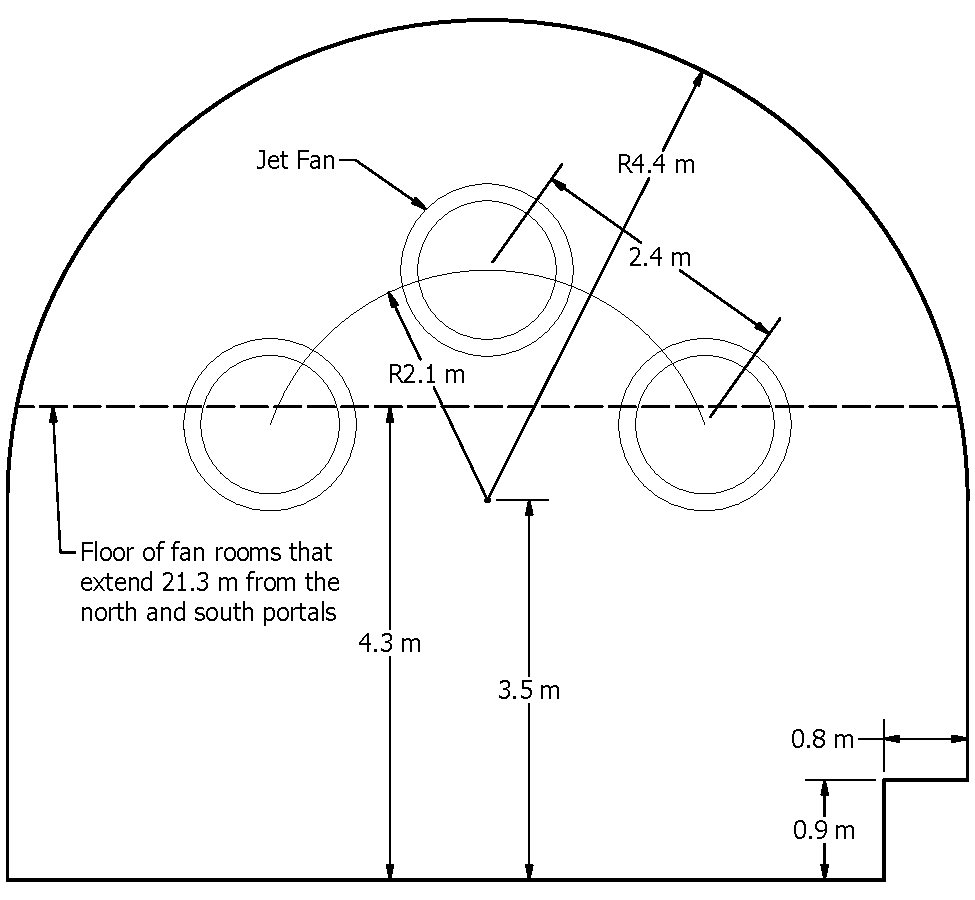
\includegraphics[width=5in]{FIGURES/Memorial_Tunnel/section}
\caption[Memorial Tunnel cross section]{Sketch of the Memorial Tunnel cross section.}
\label{Memorial_Tunnel_Cross_Section}
\end{figure}

\begin{table}[!ht]
\caption[Summary of Memorial Tunnel Experiments]{Summary of Memorial Tunnel Experiments.}
\begin{center}
\begin{tabular}{|c|c|c|c|c|}
\hline
Test     & Sequence & Heat Release  & Number   & Fan Start   \\ 
Number   & Number   & Rate (MW)     & of Fans  & Time (min)  \\ \hline \hline
501      & 15       & 20            & 0        & N/A         \\ \hline
502      & 15       & 50            & 0        & N/A         \\ \hline
605      & 17       & 10            & 1-15     & 0           \\ \hline
606A     & 17       & 10            & 0-3      & 5           \\ \hline
607      & 17       & 20            & 2-3      & 0           \\ \hline
608      & 17       & 20            & 0-4      & 2           \\ \hline
610      & 17       & 50            & 4-6      & 0           \\ \hline
611      & 17       & 50            & 0-6      & 2           \\ \hline
612B     & 17       & 50            & 0-10     & 5           \\ \hline
615B     & 17       & 100           & 0-6      & 2           \\ \hline
617A     & 17       & 10            & 1-5      & 0           \\ \hline
618A     & 17       & 20            & 0-4      & 2           \\ \hline
621A     & 17       & 100           & 2-8      & 0           \\ \hline
622B     & 17       & 50            & 0-10     & 0           \\ \hline
623B     & 18       & 20            & 1-6      & 0           \\ \hline
624B     & 18       & 50            & 0-7      & 2           \\ \hline
625B     & 18       & 100           & 3-7      & 0           \\ \hline
\end{tabular}
\end{center}
\label{tab:Memorial_Test_Matrix}
\end{table}


\subsubsection{Modeling Notes}

The simulations of the Memorial Tunnel experiments are performed with a 0.28~m uniform grid. This grid size is chosen so that the exit area of the jet fans can be approximated by a four by four array of cells. The jet fans are modeled as rectangular ducts with a specified volume flow of 42.9~m$^3$/s (91\,000~cfm). The fan speed is ramped up or down in approximately 10~s.

The 854~m tunnel is divided into 84 equal lengths. Rectangular obstructions approximate the semi-circular tunnel ceiling, vehicle silhouettes, and instrumentation packages.

The fuel is assumed to be n-heptane with a soot yield of 3.7~\% and CO yield of 1.0~\%~\cite{SFPE:Tewarson}. The heat release rates of the fires are specified as functions of time following the measured curves found in the test report.

The results of the simulations are found in Section~\ref{Memorial_Tunnel_Volume_Flow}.


\section{Montoir LNG Fires}
\label{Montoir_LNG_Fires_Description}

In 1987, British Gas, British Petroleum, Shell, Elf Aquitaine, Total CFP, and Gaz de France conducted 35~m diameter LNG pool fire experiments~\cite{Nedelka:1990}. The construction of the test facility was carried out by Gaz de France near the Montoir de Bretagne methane terminal. Three fire experiments were performed under different wind conditions. The Montoir site was selected because the ground is level and obstruction free. Wide angle radiation measurements were made at various locations around the fires, extending outwards approximately 300~m. A bund constructed of lightweight concrete and sand, approximately 1~m tall, surrounded the 35~m pool. 

A summary of the key test parameters is given in Table~\ref{Montoir_Summary}. Note that results were compiled for specific time intervals during each experiment.

\begin{table}[!ht]
\centering
\caption[Summary of the Montoir LNG Fire Experiments]{Summary of the Montoir LNG Fire Experiments.}
\label{Montoir_Summary}
\begin{tabular}{|c|c|c|c|c|c|c|c|}
\hline
                            & Time    & Burning      & Wind      & 9~m Wind & Amb.                & Rel.                & Atm.                    \\
Test                        & Interval& Rate         & Direction & Speed    & Temp.               & Hum.                & Pres.                   \\
                            & (s)     & (kg/m$^2$/s) & (deg)     & (m/s)    & ($^\circ$C)         & (\%)                & (mbar)                  \\ \hline \hline
\multirow{2}{*}{1}          & 60-100  & 0.12         & 59        & 2.5      & \multirow{2}{*}{25} & \multirow{2}{*}{53} & \multirow{2}{*}{1022}   \\  
                            & 130-170 & 0.13         & 70        & 4.8      &                     &                     &                         \\ \hline
\multirow{4}{*}{2}          & 35-50   & 0.14         & 268       & 6.8      & \multirow{4}{*}{21} & \multirow{4}{*}{54} & \multirow{4}{*}{1015}   \\
                            & 65-85   & 0.15         & 263       & 9.8      &                     &                     &                         \\
                            & 100-130 & 0.16         & 260       & 10.3     &                     &                     &                         \\
                            & 165-185 & 0.15         & 257       & 9.1      &                     &                     &                         \\ \hline
\multirow{3}{*}{3}          & 57-70   & 0.11         & 87        & 1.9      & \multirow{3}{*}{14} & \multirow{3}{*}{85} & \multirow{3}{*}{1009}   \\
                            & 90-120  & 0.13         & 79        & 3.5      &                     &                     &                         \\
                            & 130-160 & 0.13         & 82        & 4.2      &                     &                     &                         \\ \hline
\end{tabular}
\end{table}

\subsubsection{Modeling Notes}

The experiments are simulated using the specified fuel burning rates for the several time periods during each experiment. The fuel is assumed to be methane. The atmosphere is assumed to be unstable with an Obukhov length, $L=-350$, and the ground surface is roughly open with an assumed aerodynamic roughness, $z_0=0.1$~m. The relative humidity, ambient temperature and pressure, and wind speed at 9~m are specified in Table~\ref{Montoir_Summary}. 

The radiative fraction is assumed to 0.14 based on field estimates and the radiative path length is assumed to be 300~m; that is, the effective absorption coefficients of the various gas mixtures are evaluated over a distance of 300~m. 600 solid angles, rather than the default 100, are used to solve the radiative transport equation. The soot yield is assumed to be 0.01.

\begin{description}
\item[Flame Height Results:] Section~\ref{Flame Height}
\item[Flame Tilt Results:] Section~\ref{Flame Tilt}
\item[Heat Flux Results:] Section~\ref{Montoir_LNG_Fires_Heat_Flux}
\end{description}

\FloatBarrier


\section{NBS Multi-Room Experiments}
\label{NBS_Multi-Room_Description}

The National Bureau of Standards (NBS, which is now called the National Institute of Standards and Technology, NIST) Multi-Room Experiments consisted of 45 fire tests representing 9 different sets of conditions were conducted in a three-room suite (see Fig.~\ref{NBS_Drawing}). The experiments were conducted in 1985 and are described in detail in Ref.~\cite{Peacock:NBS_Multi-Room}. The suite consisted of two relatively small rooms, connected via a relatively long corridor. The fire source, a gas burner, was located against the rear wall of one of the small compartments.  Fire tests of 100~kW, 300~kW and 500~kW were conducted. For the current study, only three 100~kW fire experiments have been used, including Test~100A from Set~1, Test~100O from Set~2, and Test~100Z from Set~4. These tests were selected because they had been used in prior validation studies, and because these tests had the steadiest values of measured heat release rate during the steady-burn period.

Following is additional information provided by the test director, Richard Peacock of NIST:
\begin{description}
\item[Heat Release Rate:] In the two tests for which the door was open, the HRR during the steady-burn period measured via oxygen consumption calorimetry was 110~kW with an uncertainty of about 15~\%, consistent with the replicate measurements made during the experimental series and the uncertainty typical of oxygen consumption calorimetry. It was assumed that the closed door test (Test~100O) had the same HRR as the open door tests.
\item[Radiative Fraction:] Natural gas was used as the fuel in Test~100A. In Tests~100O and 100Z, acetylene was added to the natural gas to increase the smoke yield, and as a consequence, the radiative fraction increased. The radiative fraction of natural gas has been studied previously, whereas the radiative fraction of the acetylene/natural gas mixture has not been studied. The radiative fraction for the natural gas fire was assigned a value of 0.20, whereas a value of 0.30 was assigned for the natural gas/acetylene fires.
\item[Measurements:] Only two types of measurements conducted during the NBS test series were used in the evaluation considered here, because there was less confidence in the other measurements. The measurements considered here were the HGL temperature and depth, in which bare bead TCs were used to make these measurements. Single point measurements of temperature within the burn room were not used in the evaluation of plume or ceiling jet algorithms. This is because the geometry was not consistent in either case with the assumptions used in the model algorithms of plumes or jets. Specifically, the burner was mounted against a wall, and the room width-to-height ratio was less than that assumed by the various ceiling jet correlations.
\end{description}

\begin{figure}[p]
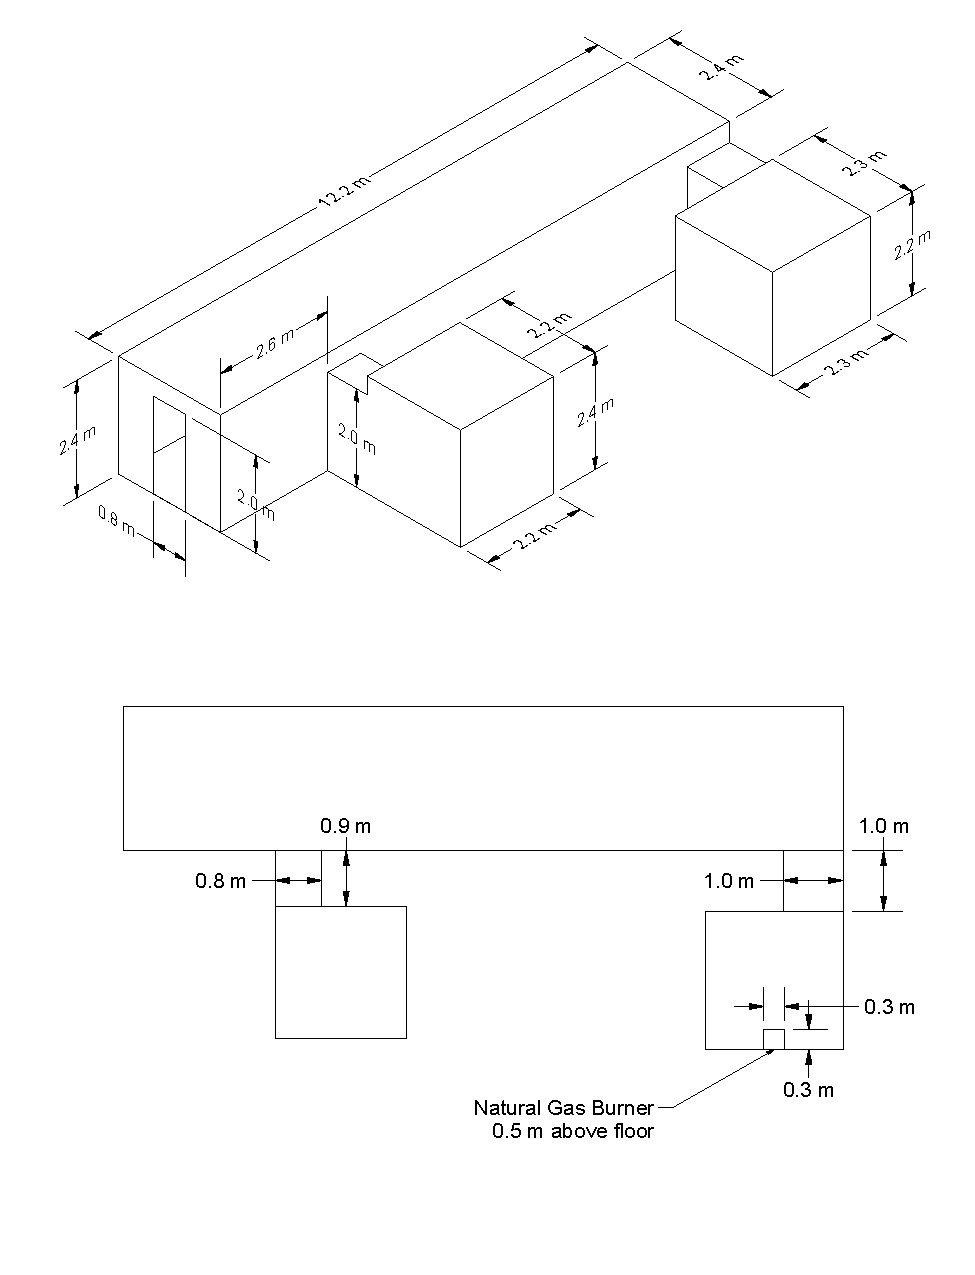
\includegraphics[width=\textwidth]{FIGURES/NBS/NBS}
\caption[Geometry of the NBS Multi-Room Experiments]{Geometry of the NBS Multi-Room Experiments.}
\label{NBS_Drawing}
\end{figure}


\section{NIST Composite Beam Experiments}
\label{NIST_Composite_Beam_Description}

A set of experiments was conducted in the Large Fire Laboratory at NIST to study the behavior of long-span steel-concrete composite floor beams designed and constructed following U.S. building codes and standards~\cite{Ramesh:TNXXXX}. The composite beam consisted of a 12.8~m long W18$\times$35 steel beam and an 16~cm thick lightweight concrete slab cast on top of 7.6~cm deep ribbed steel decking. Drawings of the compartment are shown in Figs.~\ref{NIST_Composite_Beam_Drawing_1} through \ref{NIST_Composite_Beam_Drawing_3}.

Simultaneous mechanical and fire loading was applied to the specimens. The measurements focused on evaluation of the characteristics of the fire loading, temperatures, and structural responses of the specimens to fires.

\subsubsection{Modeling Notes}

The simulations of the NIST Composite Beam experiments are performed with 5~cm grid cells and 32 meshes. The calculations are sped up by a factor of 10 using {\ct TIME\_SHRINK\_FACTOR=10}, whereby a 60~min experiment is simulated in 6~min of real time because the heat release rate is held steady for most of the experiment. The specific heats of all solid materials are reduced by a factor of 10 automatically to account for the change in time scale.

Because these experiments involve a global equivalence ratio of approximately 1, the two-step simple chemistry model is used, where soot and CO are produced when the fire becomes under-ventilated.

\begin{sidewaysfigure}[p]
\includegraphics[width=\textwidth]{FIGURES/NIST_Composite_Beam/NFRL_CompositeBeamTest_CompartmentWallLayout_1}
\caption[Elevation view of NIST Composite Beam experiments]{Elevation view of NIST Composite Beam experiments.}
\label{NIST_Composite_Beam_Drawing_1}
\end{sidewaysfigure}

\begin{sidewaysfigure}[p]
\includegraphics[width=\textwidth]{FIGURES/NIST_Composite_Beam/NFRL_CompositeBeamTest_CompartmentWallLayout_2}
\caption[Plan view of NIST Composite Beam experiments]{Plan view of NIST Composite Beam experiments.}
\label{NIST_Composite_Beam_Drawing_2}
\end{sidewaysfigure}

\begin{sidewaysfigure}[p]
\includegraphics[width=\textwidth]{FIGURES/NIST_Composite_Beam/NFRL_CompositeBeamTest_CompartmentWallLayout_3}
\caption[Side view of NIST Composite Beam experiments]{Side view of NIST Composite Beam experiments.}
\label{NIST_Composite_Beam_Drawing_3}
\end{sidewaysfigure}

\section{NIST E119 Compartment Experiments}
\label{NIST_E119_Compartment_Description}

In December 2018, three fire experiments were conducted in a compartment approximately 10.8~m wide, 7.0~m deep and 3.8~m high, constructed in the Large Fire Laboratory of NIST~\cite{Ana:TNXXXX}. The experiments were designed to test different types of floor assemblies. Two experiments, designed as replicates, lasted 15~min, and the third lasted 75~min. Four natural gas burners generated a peak heat release rate of approximately 10~MW in the 75~min experiments. The measured average upper layer gas temperature was comparable with that prescribed in the ASTM~E119 standard~\cite{E119}. Drawings of the compartment are shown in Figs.~\ref{NIST_E119_Compartment_Drawing_1} through~\ref{NIST_E119_Compartment_Drawing_3}.

\begin{sidewaysfigure}[p]
\includegraphics[width=0.65\textwidth, angle =90]{FIGURES/NIST_E119_Compartment/NIST_E119_Compartment_TCTrees}
\caption[Plan view of NIST E119 Compartment experiment]{Plan view of NIST E119 Compartment experiment.}
\label{NIST_E119_Compartment_Drawing_1}
\end{sidewaysfigure}

\begin{sidewaysfigure}[p]
\includegraphics[width=\textwidth]{FIGURES/NIST_E119_Compartment/NIST_E119_Compartment_SWall}
\caption[Elevation view of NIST E119 Compartment experiment]{Elevation view of NIST E119 Compartment experiment.}
\label{NIST_E119_Compartment_Drawing_2}
\end{sidewaysfigure}

\begin{sidewaysfigure}[p]
\includegraphics[width=\textwidth]{FIGURES/NIST_E119_Compartment/NIST_E119_Compartment_NWall}
\caption[Elevation view of NIST E119 Compartment experiment]{Elevation view of NIST E119 Compartment experiment.}
\label{NIST_E119_Compartment_Drawing_3}
\end{sidewaysfigure}

\FloatBarrier

\section{NIST Douglas Firs}
\label{NIST_Douglas_Firs_Description}

In 2009, Mell et~al. measured the burning rate and heat fluxes from individual Douglas fir trees of various sizes and moisture contents~\cite{Mell:2009}. Nine of the trees were approximately 2~m tall, and three were approximately 5~m tall. The results were presented as averages: the three 5~m trees had an average moisture content of 26~\%, three of the 2~m trees had an average moisture content of 49~\%, and the remaining six 2~m trees had a moisture content of 14~\%. The 2~m trees were ignited with a natural gas ring burner with a diameter of 80~cm and a heat release rate of 30~kW. The trees with a moisture content of 14~\% were exposed to the burner for 10~s and the 49~\% trees were exposed for 30~s. The 5~m trees were exposed to a hexagonal burner with a span of 122~cm and HRR of 130~kW for 30~s.

\subsubsection{Modeling Notes}

The trees are modeled as a collection of cylindrical Lagrangian particles. Mell~et~al.~\cite{Mell:2009} group the particles into three size classes. The pyrolysis model applied to the particles is based on TGA measurements of longleaf pine needles described in the FDS Verification Guide~\cite{FDS_Verification_Guide}, chapter ``Pyrolysis,'' Section ``TGA for a Charring Sample (Needle\_TGA).''

Measured properties of the trees are listed in Table~\ref{Properties_Trees}, and assumed properties are listed in Table~\ref{Assumed_Properties_Trees}. These assumed properties are typically for wood or cellulosic fuels. The moisture is modeled as water. The vegetation is assumed to be composed primarily of cellulose. Reference~\cite{Mell:2009} provides an estimate of the distribution of mass for the foliage, roundwood less than 3~mm in diameter, roundwood 3~mm to 6~mm, and roundwood 6~mm to 10~mm. For the 2~m trees, the distribution is approximately 64~\%, 11~\%, 10~\%, and 15~\%, respectively. For the 5~m trees, it is 60~\%, 17~\%, 12~\%, and 11~\%, respectively.

\begin{table}[ht]
\begin{center}
\caption[Measured properties for the NIST Douglas Fir Experiments]{Measured properties for the NIST Douglas Fir Experiments~\cite{Mell:2009}.}
\label{Properties_Trees}
\begin{tabular}{|l|c|c|c|c|}
\hline
Property                                & Units         & Case 1        & Case 2        & Case 3     \\ \hline \hline
Replicate Experiments                   & --            & 6             & 3             & 3          \\ \hline
Avg.~Crown Height                       & m             & 1.9           & 1.9           & 4.2        \\ \hline
Avg.~Base Height                        & m             & 0.15          & 0.15          & 0.3        \\ \hline
Avg.~Base Width                         & m             & 1.7           & 1.7           & 2.9        \\ \hline
Foliage Surface Area to Volume Ratio    & m$^{-1}$      & 3940          & 3940          & 3940       \\ \hline
Avg.~Initial Mass                       & kg            & 9.7           & 13.5          & 57.9       \\ \hline
Avg.~Moisture Fraction                  & \%            & 14            & 49            & 26         \\ \hline
Assumed Bulk Mass per Unit Volume       & kg/m$^3$      & 3.2           & 4.6           & 2.7        \\ \hline
\end{tabular}
\end{center}
\end{table}

\begin{table}
\begin{center}
\caption[Assumed properties for the NIST Douglas Fir Experiments]{Assumed properties for the NIST Douglas Fir Experiments.}
\label{Assumed_Properties_Trees}
\begin{tabular}{|l|c|c|c|}
\hline
Property                        & Units                 & Value                              & Reference                             \\ \hline \hline
Chemical Composition            & --                    & C$_{3.4}$H$_{6.2}$O$_{2.5}$        & \cite{Ritchie:1}                      \\ \hline
Heat of Combustion              & kJ/kg                 & 17700                              & \cite{Susott:FS1982}                  \\ \hline
Soot Yield                      & kg/kg                 & 0.02                               & \cite{Mell:2009}                      \\ \hline
Char Yield                      & kg/kg                 & 0.26                               & \cite{Susott:FS1982}                  \\ \hline
Specific Heat                   & kJ/(kg$\cdot$K)       & $1.1+0.0037 \, T$                  & \cite{Parker:1989}                    \\ \hline
Conductivity                    & W/(m$\cdot$K)         & 0.2                                & Assumption                            \\ \hline
Density                         & kg/m$^3$              & 514                                & \cite{Rothermel:1972}                 \\ \hline
Heat of Pyrolysis               & kJ/kg                 & 416                                & \cite{Morvan:CF2004}                  \\ \hline
\end{tabular}
\end{center}
\end{table}


\section{NIST Enclosure Experiments}
\label{NIST_Enclosure_Description}

A variety of reduced-scale and full-scale compartment fire experiments have been performed at NIST over the past few decades. The main objective of each series is to measure the concentrations of oxygen, carbon dioxide, carbon monoxide, soot, and unburned hydrocarbons in an under-ventilated compartment. These data sets also provide extreme temperature and heat flux measurements.

\subsection{NIST Reduced Scale Enclosure Experiments, 1994}
\label{NIST_RSE_1994_Description}

The NIST Reduced Scale Enclosure (RSE) was a 40~\% scale version of the ISO~9705 compartment~\cite{Bryner:1}. It measured 0.98~m wide by 1.46~m deep by 0.98~m tall. A door, centered on the smaller wall, was 0.48~m wide by 0.81~m tall.  A 15~cm diameter natural gas burner was positioned in the center of the compartment.  The burner was on a stand so that its top was 15~cm above the floor. The fires ranged from 50~kW to 600~kW. Species measurements, including CO concentration, were made near the ceiling in the front and back of the compartment.

\subsection{NIST Reduced Scale Enclosure Experiments, 2007}
\label{NIST_RSE_2007_Description}

Another set of reduced-scale compartment experiments was conducted in 2007 at NIST~\cite{Bundy:1}. The compartment was similar in dimension: 0.95~m wide by 1.42~m deep by 0.98~m tall with the exact same door dimensions. Four different burner types were used: a 13~cm square sand burner, a 25~cm square liquid fuel burner, a spray nozzle into 0.4~m diameter circular pan, and a 60~cm diameter circular pan. Six different fuels were used: natural gas; heptane, methanol, ethanol and toluene liquids; and solid polystyrene beads. The fires ranged from 15~kW to 425~kW, but only fires greater than 190~kW were used for comparison because the smaller fires produced no significant CO. Measurements of O$_2$, CO$_2$, CO, soot, and unburned hydrocarbon concentration were made near the ceiling in the front and back of the compartment.

\begin{table}[!ht]
\caption{Summary of NIST Reduced-Scale Experiments, 2007.}
\begin{center}
\begin{tabular}{|c|c|c|c|c|c|}
\hline
Test   &  Fuel         &  Fuel           & Peak        &  Burner       &  Doorway          \\
No.    &  Type         &  Formula        & HRR (kW)    &  Size (m$^2$) &  Opening (cm)     \\ \hline \hline
1      &  Natural Gas  &  CH$_4$         & 190         &  0.017        &  48               \\ \hline
2      &  Natural Gas  &  CH$_4$         & 395         &  0.017        &  48               \\ \hline
3      &  Natural Gas  &  CH$_4$         & 410         &  0.017        &  48               \\ \hline
4      &  Heptane      &  C$_7$H$_{16}$  & 375         &  0.063        &  48               \\ \hline
5      &  Heptane      &  C$_7$H$_{16}$  & 220         &  0.063        &  24               \\ \hline
6      &  Natural Gas  &  CH$_4$         & 420         &  0.063        &  24               \\ \hline
7      &  Heptane      &  C$_7$H$_{16}$  & 340         &  0.063        &  48               \\ \hline
10     &  Toluene      &  C$_7$H$_8$     & 340         &  0.063        &  48               \\ \hline
11     &  Ethanol      &  C$_2$H$_6$O    & 335         &  0.126        &  48               \\ \hline
12     &  Methanol     &  CH$_4$O        & 305         &  0.126        &  48               \\ \hline
15     &  Heptane      &  C$_7$H$_{16}$  & 375         &  0.126        &  48               \\ \hline
16     &  Polystyrene  &  C$_8$H$_8$     & 360         &  0.283        &  48               \\ \hline
\end{tabular}
\end{center}
\label{tab:NIST_RSE_Exp}
\end{table}


\subsection{NIST Full-Scale Enclosure Experiments, 2008}
\label{NIST_FSE_2008_Description}

The NIST FSE (2008) Experiments were conducted in an ISO~9705 compartment~\cite{Lock:1}. The compartment was 2.4~m wide by 3.6~m long by 2.4~m high with a 2~m high door at one end (Fig.~\ref{NIST_FSE_2008_Drawing}). The door width varied between 0.1~m and 0.8~m. The experiments were designed to study the effects of fuel type, fuel distribution, and vent size on under-ventilated compartment fires. Twenty-seven of the thirty experiments were simulated, which included 7 different fuels, 3 fuel sources, and 4 ventilation openings. The three experiments not simulated had several malfunctions of equipment such that the data could not be trusted.

Peak heat release rates ranged from approximately 100~kW to 2.5~MW. Table~\ref{tab:NIST_FSE_Exp} provides a summary of the experiments. Species concentrations and temperature measurements were made at the front and rear of the compartment.



\begin{figure}[!ht]
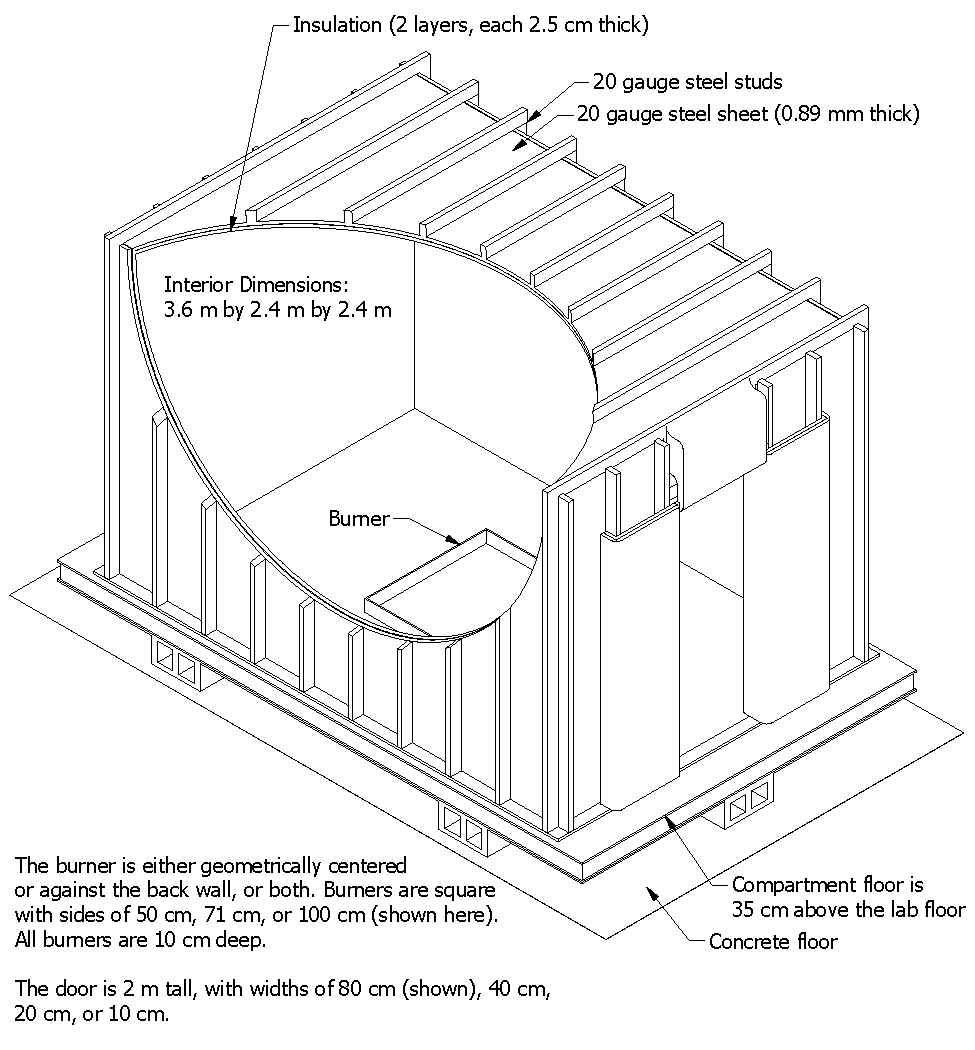
\includegraphics[width=\textwidth]{FIGURES/NIST_FSE_2008/NIST_FSE_2008_Drawing}
\caption[Geometry of the compartment used in the NIST Full-Scale Enclosure experiments]{Geometry of the compartment used in the NIST Full-Scale Enclosure (FSE) experiments.}
\label{NIST_FSE_2008_Drawing}
\end{figure}

\begin{table}[!ht]
\caption[Summary of NIST FSE Experiments selected for model validation]{Summary of NIST FSE Experiments selected for model validation.}
\begin{center}
\begin{tabular}{|l|l|c|c|c|c|c|}
\hline
Test          &  Fuel         &  Fuel             &  Fuel      &  No.~of   &  Burner       &  Doorway          \\
Name          &  Type         &  Formula          &  Mass (kg) &  Burners  &  Size (m$^2$) &  Opening (cm)     \\ \hline \hline
ISONG3        &  Natural Gas  &  CH$_4$           &            &  1        &  1.0          &  80               \\ \hline
ISOHept4      &  Heptane      &  C$_7$H$_{16}$    &  Pool Fed  &  1        &  1.0          &  80               \\ \hline
ISOHept5      &  Heptane      &  C$_7$H$_{16}$    &  Pool Fed  &  1        &  1.0          &  40               \\ \hline
ISOHept8      &  Heptane      &  C$_7$H$_{16}$    &  10        &  1        &  0.5          &  20               \\ \hline
ISOHept9      &  Heptane      &  C$_7$H$_{16}$    &  20        &  1        &  0.5          &  20               \\ \hline
ISONylon10    &  Nylon        &  C$_6$H$_{11}$NO  &  10        &  1        &  0.5          &  20               \\ \hline
ISOPP11       &  Propylene    &  C$_3$H$_6$       &  10        &  1        &  0.5          &  20               \\ \hline
ISOHeptD12    &  Heptane      &  C$_7$H$_{16}$    &  20        &  2        &  0.25         &  20               \\ \hline
ISOHeptD13    &  Heptane      &  C$_7$H$_{16}$    &  20        &  2        &  0.25         &  20               \\ \hline
ISOPropD14    &  Propanol     &  C$_3$H$_8$O      &  24        &  2        &  0.25         &  20               \\ \hline
ISOProp15     &  Propanol     &  C$_3$H$_8$O      &  24        &  1        &  0.5          &  20               \\ \hline
ISOStyrene16  &  Styrene      &  C$_8$H$_8$       &  10        &  1        &  0.5          &  20               \\ \hline
ISOStyrene17  &  Styrene      &  C$_8$H$_8$       &  30        &  1        &  1.0          &  20               \\ \hline
ISOPP18       &  Propylene    &  C$_3$H$_6$       &  20        &  2        &  0.5          &  20               \\ \hline
ISOHept19     &  Heptane      &  C$_7$H$_{16}$    &  20        &  1        &  0.5          &  20               \\ \hline
ISOToluene20  &  Toluene      &  C$_7$H$_8$       &  17        &  1        &  0.5          &  20               \\ \hline
ISOStyrene21  &  Styrene      &  C$_8$H$_8$       &  15        &  1        &  0.5          &  20               \\ \hline
ISOHept22     &  Heptane      &  C$_7$H$_{16}$    &  Spray     &  1        &  0.5          &  20               \\ \hline
ISOHept23     &  Heptane      &  C$_7$H$_{16}$    &  Spray     &  1        &  0.5          &  10               \\ \hline
ISOHept24     &  Heptane      &  C$_7$H$_{16}$    &  Spray     &  1        &  0.5          &  10               \\ \hline
ISOHept25     &  Heptane      &  C$_7$H$_{16}$    &  Spray     &  1        &  0.5          &  40               \\ \hline
ISOHept26     &  Heptane      &  C$_7$H$_{16}$    &  Spray     &  1        &  0.5          &  40               \\ \hline
ISOHept27     &  Heptane      &  C$_7$H$_{16}$    &  Spray     &  1        &  0.5          &  10               \\ \hline
ISOHept28     &  Heptane      &  C$_7$H$_{16}$    &  Spray     &  1        &  0.5          &  20               \\ \hline
ISOToluene29  &  Toluene      &  C$_7$H$_8$       &  Spray     &  1        &  0.5          &  20               \\ \hline
ISOPropanol30 &  Propanol     &  C$_3$H$_8$O      &  Spray     &  1        &  0.5          &  20               \\ \hline
ISONG32       &  Natural Gas  &  CH$_4$           &            &  1        &  0.28         &  20               \\ \hline
\end{tabular}
\end{center}
\label{tab:NIST_FSE_Exp}
\end{table}

\subsection{Modeling Notes}

In the simulations of all of the NIST enclosure experiments, it is assumed that the combustion can be simplified to two fast reactions, the first converting fuel to CO and soot, and the second converting CO and soot to CO$_2$. By default, 2/3 of the carbon in the fuel is converted to CO in the first step, the remaining 1/3 to soot. The heats of combustion for the reactions are calculated directly from the heats of formation of the individual molecules. For cases where the fuel molecule is not pre-defined in FDS (e.g., styrene), the fuel's enthalpy of formation is specified. For cases where the fuel's enthalpy of formation is not known (e.g. nylon), the heat of combustion that is reported for complete combustion is specified in a single reaction test case, from which an effective enthalpy of formation is reported\footnote{The FDS diagnostic output (.out) file contains detailed information about the reaction stoichiometry, heats of combustion, and enthalpies of formation.} and then used in the actual two-step reaction scheme.

In the experiments, the heat release rate was measured via oxygen consumption calorimetry. In the simulations, the mass loss rate of fuel was specified by taking the measured HRR and dividing by the heats of combustion listed in Ref.~\cite{SFPE:Tewarson}.

In all simulations, the model geometry included the compartment interior plus a comparable volume at the exterior to allow for a natural flow into and out of the compartment.

Also, in all simulations, the fire suppression algorithm has been turned off ({\ct SUPPRESSION=.FALSE.}). The reason for this is that the suppression algorithm is not able to distinguish viability of a fire that is close to the point of extinction. Research continues in this area.


\FloatBarrier


\section{NIST Helium Experiments}
\label{NIST_Helium_Description}

Eighteen experiments were conducted at NIST in which helium was released over a lengthy time period inside of a 1.5~m by 1.5~m by 0.75~m plexiglass box with one or two small leakage holes~\cite{Pitts:2011}. The experiments were intended to represent the release of hydrogen from passenger vehicle fuel cell inside of a residential garage. Test parameters included the release rate and length, the location of the release, and the size and location of the leakage. Measurements were made of the helium concentration in a rake at seven locations over the height of the compartment during the release and for a period of up to 11 hours post-release.

Test variables included all permutations of the leak rate and time (14.8~L/min over 3600~s or 3.71~L/min over 14400~s), leak location (on the floor at the center of the compartment, on the floor at the center of the rear wall, and 2.5~cm below the ceiling at the center of the compartment), and the leak area (2.4~cm by 2.4~cm at the center of the front wall, 3.05~cm by 3.05~cm at the center of the front wall, and a pair of 2.15~cm by 2.15~cm centered on the front wall 2.5~cm from the floor and ceiling).

Leakage areas were square holes under 10~cm$^2$ in area.  Attempting to resolve flows through these holes would have required very small grid cells in the vicinity of the holes.  Instead, the FDS HVAC model was used.  For each leakage hole a pair of HVAC ducts was defined over a height of two grid cells (one grid cell height for each vent).  Each duct was assigned one-half the leakage area and the experimentally determined orifice flow coefficient. This approach enabled bi-directional flow to occur at the leakage vent as occurred during each test following the termination of the helium release.



\section{NIST/NRC Compartment Experiments}
\label{NIST_NRC_Description}

These experiments, sponsored by the US NRC and conducted at NIST, consisted of 15 large-scale experiments performed in June 2003. All 15 tests were included in the validation study. The experiments are documented in Ref.~\cite{Hamins:SP1013-1}. The fire sizes ranged from 350 kW to 2.2 MW in a compartment with dimensions 21.7~m by 7.1~m by 3.8~m high, designed to represent a compartment in a nuclear power plant containing power and control cables. A diagram of the test structure is displayed in Figure~\ref{NIST_NRC_Drawing}.

\begin{figure}[p]
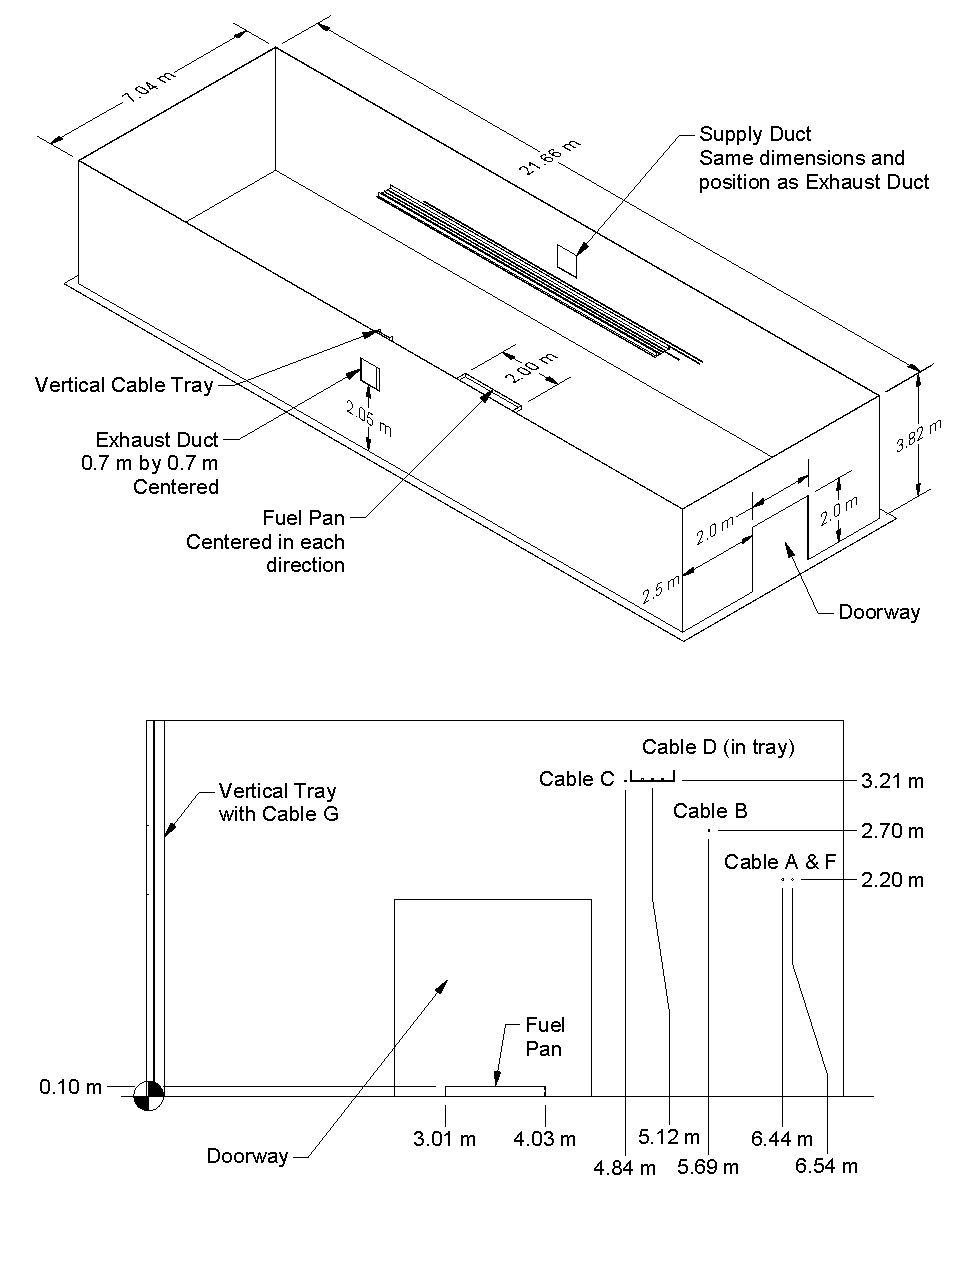
\includegraphics[width=\textwidth]{FIGURES/NIST_NRC/NIST_NRC_Drawing}
\caption[Geometry of the NIST/NRC Experiments]{Geometry of the NIST/NRC Experiments.}
\label{NIST_NRC_Drawing}
\end{figure}

The walls and ceiling were covered with two layers of marinate boards, each layer 0.0125~m thick. The floor
was covered with one layer of gypsum board on top of a layer of plywood. Thermo-physical and optical properties of the marinate
and other materials used in the compartment are given in Ref.~\cite{Hamins:SP1013-1}. The room had one door and a mechanical air injection and extraction
system. Ventilation conditions, the fire size, and fire location were varied. Numerous measurements (approximately 350 per test) were made including
gas and surface temperatures, heat fluxes and gas velocities.

Following are some notes provided by Anthony Hamins, who conducted the experiments:
\begin{description}
\item[Natural Ventilation:] The compartment had a 2~m by 2~m door in the middle of the west wall. Some of the tests had a closed door and no mechanical
ventilation (Tests 2, 7, 8, 13, and 17), and in those tests the measured compartment leakage was an important consideration. The test report lists leakage
areas based on measurements performed prior to Tests 1, 2, 7, 8, and 13. For the closed door tests, the leakage area used in the simulations was
based on the last available measurement. The chronological order of the tests differed from the numerical order.
For Test 4, the leakage area measured before Test 2 was used. For Tests 10 and 16, the leakage area
measured before Test 7 was used.
\item[Mechanical Ventilation:] The mechanical ventilation and exhaust was used during Tests 4, 5, 10, and 16, providing about 5 air changes per hour. The
door was closed during Test 4 and open during Tests 5, 10, and 16. The supply duct was positioned on the south wall, about 2~m off the floor. An
exhaust duct of equal area to the supply duct was positioned on the opposite wall at a comparable location. The flow rates through the supply and
exhaust ducts were measured in detail during breaks in the testing, in the absence of a fire. During the tests, the flows were monitored with single
bi-directional probes during the tests themselves.
\item[Heat Release Rate:] A single nozzle was used to spray liquid hydrocarbon fuels onto a 1~m by 2~m fire pan that was about 0.1~m deep. The test plan
originally called for the use of two nozzles to provide the fuel spray. Experimental observation suggested that the fire was less unsteady with the
use of a single nozzle. In addition, it was observed that the actual extent of the liquid pool was well-approximated by a 1~m circle in the
center of the pan. For safety reasons, the fuel flow was terminated when the lower-layer oxygen concentration
dropped to approximately 15~\% by volume.
The fuel used in 14 of the tests was heptane, while toluene was used for one test. The HRR was
determined using oxygen consumption calorimetry. The recommended uncertainty values
were 17~\% for all of the tests.
\item[Radiative Fraction:]  The values of radiative fraction and its uncertainty were reported as
\num{0.44 \pm 0.07} and \num{0.40 \pm 0.09} for heptane and toluene, respectively.
\item[Soot Yield:]  The values of the soot yield and its uncertainty were reported as \SI{0.0149 \pm 0.0033}{kg/kg}
and \SI{0.195 \pm 0.052}{kg/kg} for heptane and toluene, respectively.
\end{description}


\FloatBarrier

\section{NIST/NRC Corner, Wall, and Cabinet Experiments}
\label{NIST_NRC_Corner_Wall_Cabinet_Description}

In the summer of 2017, experiments were conducted in a large compartment in the NIST large fire laboratory on behalf of the U.S. Nuclear Regulatory Commission. There were two sets of experiments. In the first set, conducted in July, 2017, a natural gas burner was positioned either in a corner or against a wall, and gradually moved outward. In the second set of experiments, conducted in September, 2017, a natural gas burner was placed inside one of two steel cabinets meant to represent typical industrial-scale electrical enclosures.

The compartment for all experiments was 11~m long, 7~m wide, and 3.8~m high. The long dimension of the compartment ran east-west. A 1.8~m wide, 2.4~m high door was centered on the east (short) wall.

All of the fires were fueled by one or more 30.5~cm (1~ft) square natural gas burners. Each burner was essentially a steel box, 30.5~cm square in plan and 15~cm deep, fueled from below. The lip of the burner was 2.5~cm (1~in) wide. A 2.5~cm thick piece of Kaowool insulation was placed under a steel mesh to form the surface of the burner.

\subsection{Wall and Corner Effects}

Six large compartment experiments~\cite{McGrattan:TN1984} were conducted in July, 2017, where four natural gas burners were positioned (1) in a corner and (2) against a wall, and then moved outward in stages until the corner or wall effect became negligible. The quad burner was 60~cm by 60~cm and the burner surface was 54~cm above the floor. The corner fire was located in the southwest corner of the large compartment. The wall fire was centered on the south (long) wall.

The experiments began with the quad burner in the corner or against the wall for the first 30~min. At 30~min, the burner was moved so that its edge(s) was 10~cm away from the wall(s). It remained for 15~min, after which it was moved to 20~cm, 30~cm, 50~cm, 100~cm, and 160~cm, each time remaining 15~min for a total experiment time of 2~h.

A three-dimensional array of thermocouples was positioned on a track mounted to the ceiling above the burner. The purpose of this array was to measure maximum plume temperatures at heights of 2.1~m, 2.7~m, and 3.4~m above the floor. As the burner moved, the thermocouple array moved with it. For the corner fire experiments, when the burner was at the 0~cm, 10~cm, and 20~cm positions, the thermocouple array overhead remained at its original location in the corner. As the burner moved beyond 20~cm, the thermocouple array was moved the same amount so that the burner was always below the array in the same position. In other words, for the corner fire experiments, after the center point of the burner reached the point directly below the position 18 on the diagram below, the burner and array moved together, maintaining their relative position.

The experimental data consists primarily of thermocouple measurements. The key to the column names are as follows:
\begin{itemize}
\item TC-AG-01 through TC-AG-29 are the thermocouples at the top of the cage, 46~cm below the ceiling (see pattern below).
\item TC-BG-01 through TC-BG-29 are the thermocouples at the mid-level of the cage, 107 cm below the ceiling (see pattern below).
\item TC-CG-01 through TC-CG-29 are the thermocouples at the bottom of the cage, 168 cm below the ceiling (see pattern below).
\item TC-WT-01 through TC-WT-13 are the thermocouples of the vertical array called the West Tree. The array was 2.75 m from the west (short) wall and 3.5 m from the south (long) wall. TC-WT-01 was located 2 cm below the ceiling, and the rest were spaced 30 cm apart.
\item TC-ET-01 through TC-ET-13 are the thermocouples of the East Tree. The array was 2.75 m from the east (short) wall and 3.5 m from the south (long) wall. TC-ET-01 was located 2 cm below the ceiling, and the rest were spaced 30 cm apart.
\item TC-C-01 through TC-C-11 are the thermocouples 2 cm from the corner above the corner fire. TC-C-01 was located 2 cm below the ceiling, and the rest were spaced 30 cm apart.
\item TC-W-01 through TC-W-11 are the thermocouples 2 cm from the wall above the wall fire. TC-W-01 was located 2 cm below the ceiling, and the rest were spaced 30 cm apart.
\item HRR (cal) is the heat release rate of the fire as measured using oxygen consumption calorimetry. HRR (NG) is the heat release rate determined from the mass flow rate of natural gas.
\end{itemize}

\begin{figure}[!ht]

\begin{center}
\setlength{\unitlength}{1in}
\begin{picture}(5.5,4.5)
\multiput(0,0)(0.5,0.0){10}{\line(0,1){4.5}}
\multiput(0,0)(0.0,0.5){10}{\line(1,0){4.5}}
\multiput(0,0)(1.0,0.0){5}{\multiput(0,0)(0.0,1.0){5}{\circle*{0.075}}}
\multiput(0.5,0.5)(1.0,1.0){4}{\circle*{0.075}}
\put(0.1,0.1){1}
\put(0.1,1.1){7}
\put(0.1,2.1){13}
\put(0.1,3.1){19}
\put(0.1,4.1){25}
\put(1.1,0.1){2}
\put(1.1,1.1){8}
\put(1.1,2.1){14}
\put(1.1,3.1){20}
\put(1.1,4.1){26}
\put(2.1,0.1){3}
\put(2.1,1.1){9}
\put(2.1,2.1){15}
\put(2.1,3.1){21}
\put(2.1,4.1){27}
\put(3.1,0.1){4}
\put(3.1,1.1){10}
\put(3.1,2.1){16}
\put(3.1,3.1){22}
\put(3.1,4.1){28}
\put(4.1,0.1){5}
\put(4.1,1.1){11}
\put(4.1,2.1){17}
\put(4.1,3.1){23}
\put(4.1,4.1){29}
\put(0.6,0.6){6}
\put(1.6,1.6){12}
\put(2.6,2.6){18}
\put(3.6,3.6){24}
\put(5.25,2){\vector(0,-1){2}}
\put(5.25,2.5){\vector(0,1){2}}
\put(5.25,2.25){\makebox(0,0){0.91 m (36 in)}}
\put(2.25,-0.25){\makebox(0,0){South Wall}}
\end{picture}
\end{center}
\vspace{0.2in}
\caption[Diagram of thermocouple layout for NIST/NRC Corner Effects experiments]{Diagram of thermocouple layout for NIST/NRC Corner Effects experiments.}
\label{TC_pattern}

\end{figure}

The East and West Tree thermocouples were used to estimate the height of the hot gas layer (HGL), and the average temperatures of the upper and lower layers. Also, the three horizontal arrays of thermocouples above the burner were processed by first taking a 2~min running average of each TC, and then choosing the maximum value for each of the three elevations above the fire. These were taken as approximate centerline plume temperatures at each height. These experimental files are labelled with ``HGL'' and ``Plume'', respectively.

\subsection{Cabinet Effects}

In this second series of experiments, conducted in September, 2017, two different mock steel cabinets were used. Each cabinet was constructed of 12 gauge (2.8~mm or 7/64~in) steel plate with openings as shown in Figs.~\ref{Large_Cabinet} and \ref{Medium_Cabinet}. The large cabinet was nominally 0.9~m by 0.9~m by 2.1~m and the medium size cabinet was 0.6~m by 0.6~m by 2.1~m. The openings near the top of each cabinet were sometimes covered with a steel grill, shown in Fig.~\ref{cabinet_grill}.

\begin{figure}[p]
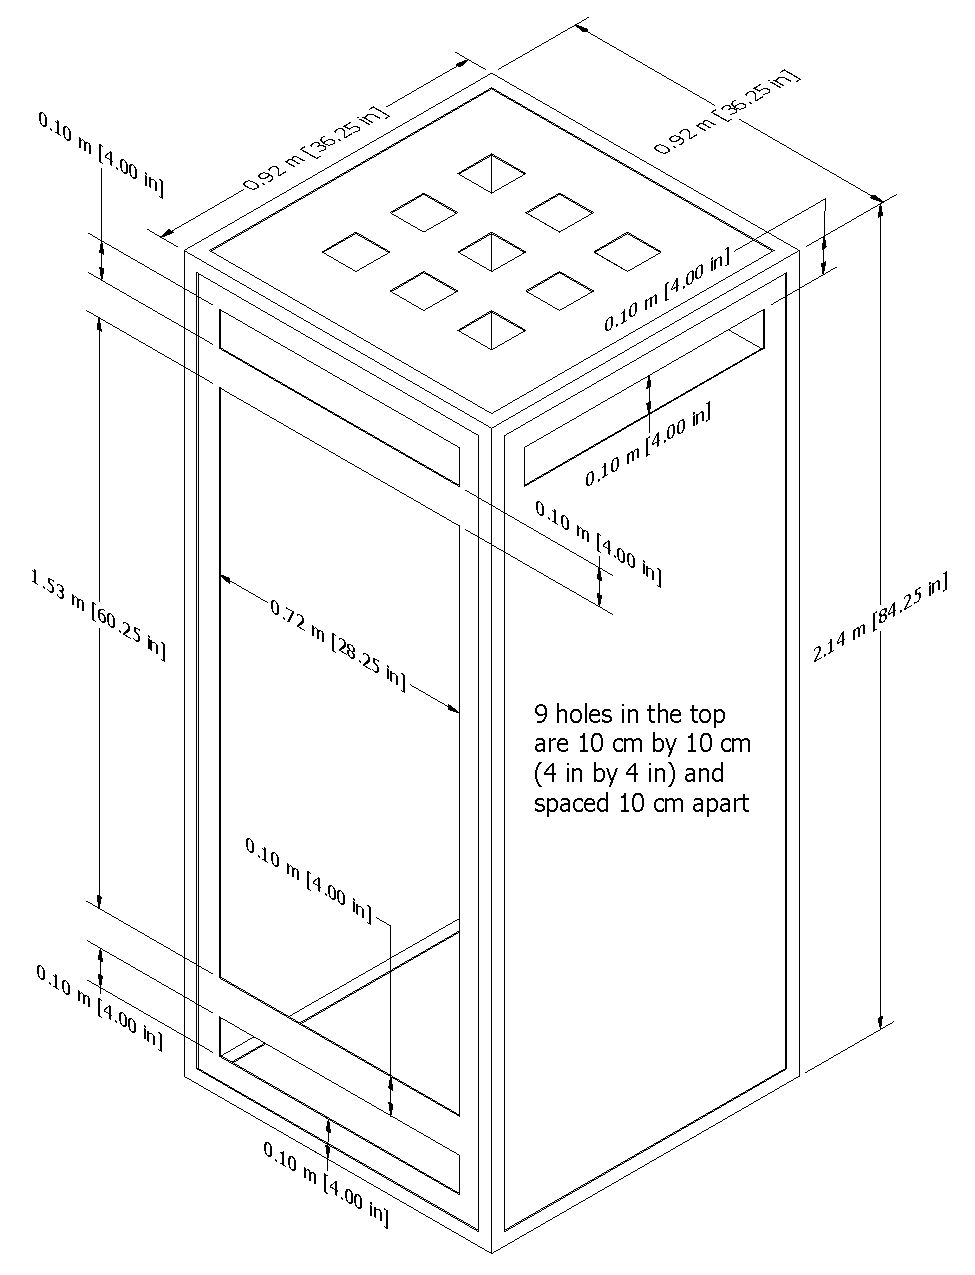
\includegraphics[width=\textwidth]{FIGURES/NIST_NRC_Corner_Effects/Cabinet_3x3x7}
\caption[Large cabinet drawing, NIST/NRC Corner Effects Experiments]{Large cabinet drawing, NIST/NRC Corner Effects Experiments.}
\label{Large_Cabinet}
\end{figure}

\begin{figure}[p]
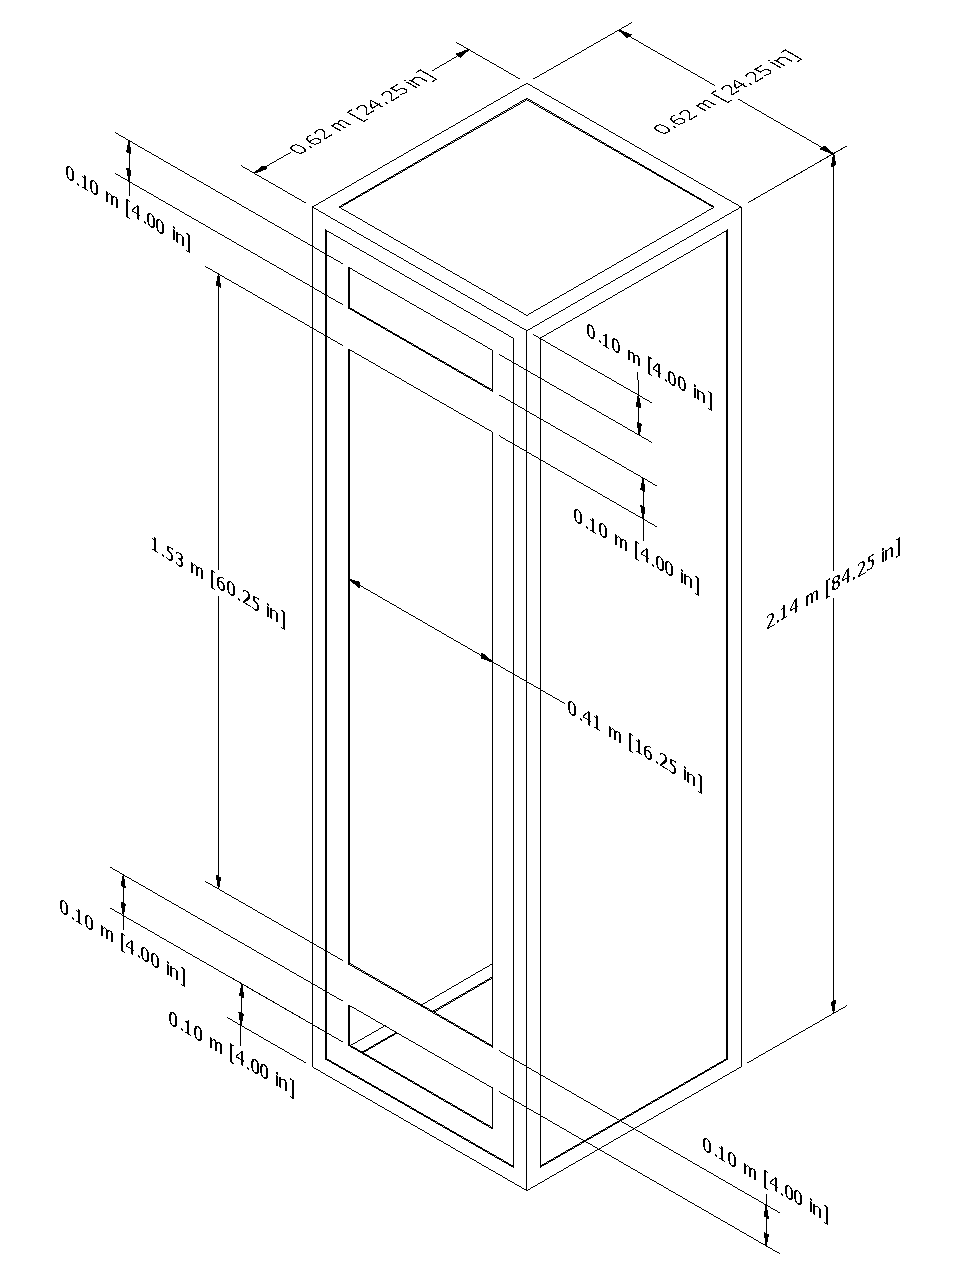
\includegraphics[width=\textwidth]{FIGURES/NIST_NRC_Corner_Effects/Cabinet_2x2x7}
\caption[Medium-sized cabinet drawing, NIST/NRC Corner Effects Experiments]{Medium-sized cabinet drawing, NIST/NRC Corner Effects Experiments.}
\label{Medium_Cabinet}
\end{figure}

\begin{figure}[!ht]
\includegraphics[width=\textwidth]{FIGURES/NIST_NRC_Corner_Effects/grill_drawing}
\caption[Cabinet grill, NIST/NRC Corner Effects Experiments]{Cabinet grill, NIST/NRC Corner Effects Experiments.}
\label{cabinet_grill}
\end{figure}


For the first set of experiments (1-6), the large cabinet was positioned with its front opening facing eastward towards the opening of the test compartment. Its left side was 1.8~m from the south wall and its front side was 5.8~m from the east wall. Two 0.3~m by 0.3~m natural gas burners were placed side by side in the cabinet from the perspective of the cabinet front opening. The top of the burner was 50~cm above the floor of the cabinet. For Tests~1-4, the front door of the cabinet was closed, and the heat release rate was initially set to 50~kW for 30~min, then it was increased to 100~kW for 15~min, 200~kW for 15~min, and 400~kW for 15~min. For Tests~5-6, the front door was opened, and the heat release rate was set to 200~kW, 400~kW, and 700~kW for 15~min each, and then 1000~kW for 5~min, a total of 50~min.

In the second set of experiments (7-10), the medium-sized cabinet was positioned so that its front was the same distance from the east wall as the large cabinet, and its left side was 2.0 m (6.5 ft) from the south wall. A single 30~cm by 30~cm gas burner was centered within. For the closed door tests, the heat release rate was 25~kW, 50~kW, 100~kW, and 200~kW, each for 15~min. For the open door tests, the heat release rate was 40~kW, 80~kW, 200~kW, and 325~kW, each for 15~min.

In the third set of experiments (11-12), the cabinet was removed, and two 30~cm by 30~cm burners were spaced 0.9~m (3~ft) apart, side to side. One of the burners was centered under the array of thermocouples. Both burners were 2.0~m from the south wall. These experiments used the same heat release rate sequence as the open and closed door large cabinet experiments.

The data files for these experiments are labelled, {\ct NIST\_NRC\_Cabinet\_Test\_n.csv}. These files contain the same measurement positions as the corner and wall experiments, with the following additional measurements:
\begin{itemize}
\item PT-1 through PT-8 are plate thermometers positioned 0.6~m (2 ft) from each side of the cabinet at heights of 0.8~m (2.5~ft) and 1.4~m (4.5~ft). PT-1 is the upper plate on the left side. PT-2 is lower left. PT-3 is upper back. PT-4 is lower back. PT-5 is upper front. PT-6 is lower front. PT-7 is upper right. PT-8 is lower right.
\item STC-1 through STC-6 are sheathed thermocouples within the cabinet, 15 cm (6 in) from the left side, centered. STC-1 is 6~cm (2.5~in) from the top. STC-2 through STC-6 are 30~cm, 60~cm, 90~cm, 120~cm, and 150~cm from the top, respectively.
\item TC-Cab is a single 24 gauge Type K thermocouple welded to the center of the back side on the outside of the cabinet. For Test~11, this TC was placed just under the Kaowool surface of the burner, and for Test~12, it was placed just above the surface.
\end{itemize}
The three dimensional array of thermocouples used in the wall and corner experiments was positioned over the front of the cabinet, such that TC positions 1, 7, 13, 19, and 25 in Fig.~\ref{TC_pattern} were just above the upper front edge of the cabinet.

The test matrix is as follows:
\begin{table}[!ht]
\caption{Summary of NIST/NRC Cabinet Experiments.}
\begin{center}
\begin{tabular}{|c|c|c|c|l|l|}
\hline
Test   & Cabinet    & Front Door & Top Vents        & Upper Side Vents                   & HRR (kW)               \\ \hline \hline
1      & Large      & Closed     & Closed           & Grill                              & 50, 100, 200, 400      \\ \hline
2      & Large      & Closed     & All open         & Grill                              & 50, 100, 200, 400      \\ \hline
3      & Large      & Closed     & Closed           & Front open, all others closed      & 50, 100, 200, 400      \\ \hline
4      & Large      & Closed     & Closed           & Front and back open, others closed & 50, 100, 200, 400      \\ \hline
5      & Large      & Open       & Closed           & Front and back open, others closed & 200, 400, 700, 1000    \\ \hline
6      & Large      & Open       & Open             & All open                           & 200, 400, 700, 1000    \\ \hline
7      & Medium     & Closed     & Closed           & Grill                              & 25, 50, 100, 200       \\ \hline
8      & Medium     & Closed     & Closed           & Open                               & 25, 50, 100, 200       \\ \hline
9      & Medium     & Open       & Closed           & Open                               & 40, 80, 200, 325       \\ \hline
10     & Medium     & Open       & Closed           & Closed                             & 40, 80, 200, 325       \\ \hline
11     & None       & N/A        & N/A              & N/A                                & 200, 400, 700, 1000    \\ \hline
12     & None       & N/A        & N/A              & N/A                                & 50, 100, 200, 400      \\ \hline
\end{tabular}
\end{center}
\label{tab:NIST_Cabinet_Experiments}
\end{table}


\FloatBarrier

\section{NIST/NRC OLIVE-Fire Experiments}
\label{NIST_NRC_OLIVE-Fire_Description}

In March, 2022, experiments were conducted at NIST to determine the maximum heat release rate that a fire can reach within steel electrical enclosures~\cite{OLIVE-Fire:2022}. OLIVE is an acronym for \underline{O}xygen-\underline{L}imited Fires \underline{I}nside Under-\underline{V}entilated \underline{E}nclosures. Photographs of the enclosures are shown in Fig.~\ref{NIST_NRC_OLIVE_Photos}. The enclosures were pressure-tested before and after the experiments to determine the leakage and vent opening areas. These opening areas are a key parameter in the numerical modeling.

Thirty-two experiments were conducted; twenty-one of which were fueled by a natural gas burner. The others involved a variety of plastics and electrical cables. Eighteen of the natural gas experiments were chosen for simulation. The natural gas cases not chosen had unexpectedly large gaps between the steel panels open up during the experiment. The leakage throught these gaps could not be measured.

\begin{figure}[p]
\begin{tabular*}{\textwidth}{l@{\extracolsep{\fill}}r}
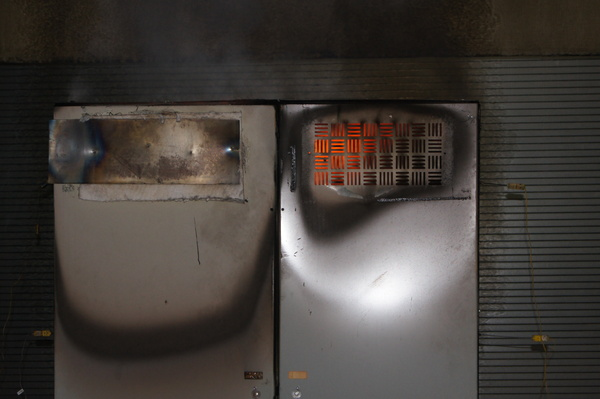
\includegraphics[height=2.0in]{FIGURES/NIST_NRC_OLIVE-Fire/Test_31_photo} &
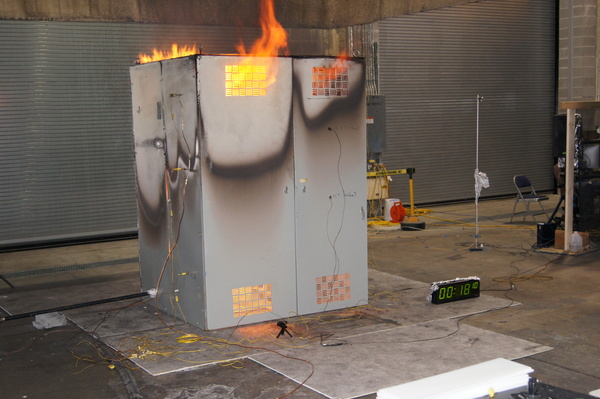
\includegraphics[height=2.0in]{FIGURES/NIST_NRC_OLIVE-Fire/Test_12_photo} \\
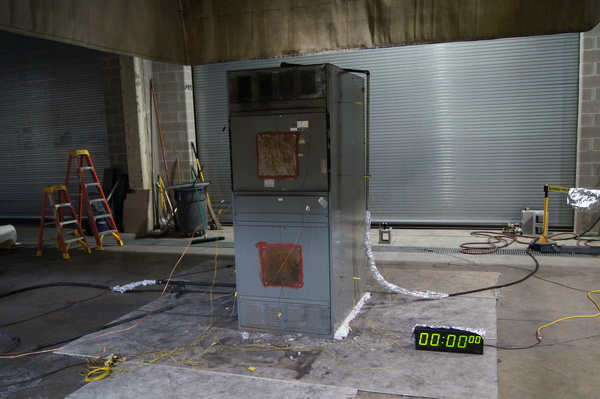
\includegraphics[height=2.0in]{FIGURES/NIST_NRC_OLIVE-Fire/Test_17_photo} &
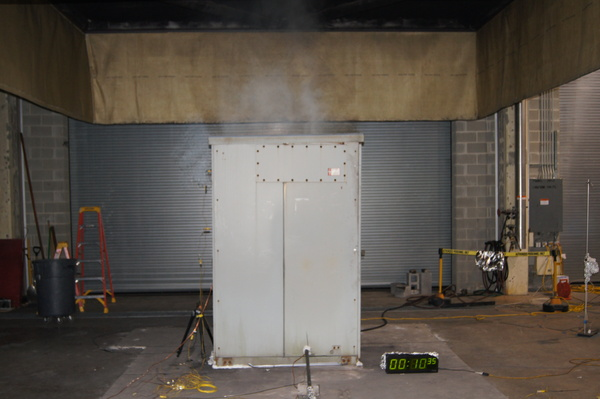
\includegraphics[height=2.0in]{FIGURES/NIST_NRC_OLIVE-Fire/Test_26_photo} \\
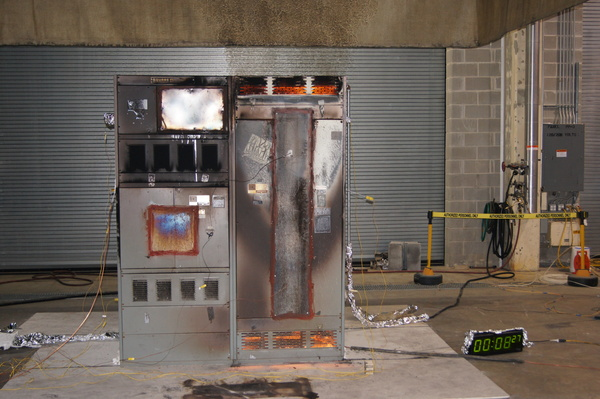
\includegraphics[height=2.0in]{FIGURES/NIST_NRC_OLIVE-Fire/Test_8_photo} &
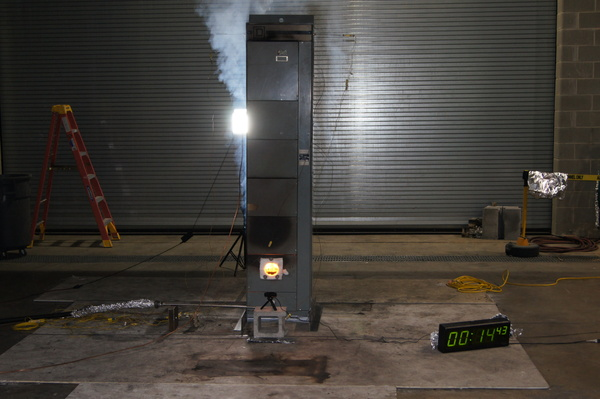
\includegraphics[height=2.0in]{FIGURES/NIST_NRC_OLIVE-Fire/Test_9_photo} \\
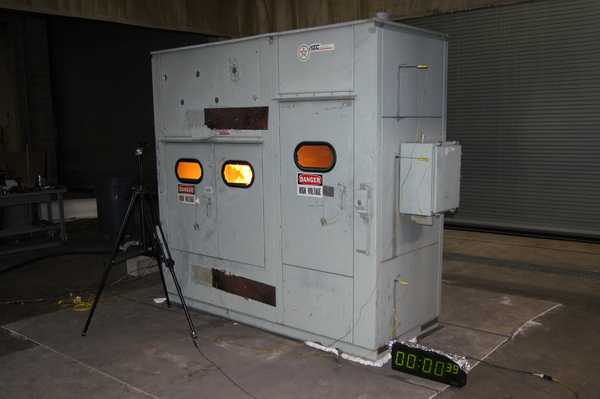
\includegraphics[height=2.0in]{FIGURES/NIST_NRC_OLIVE-Fire/Test_23_photo} &
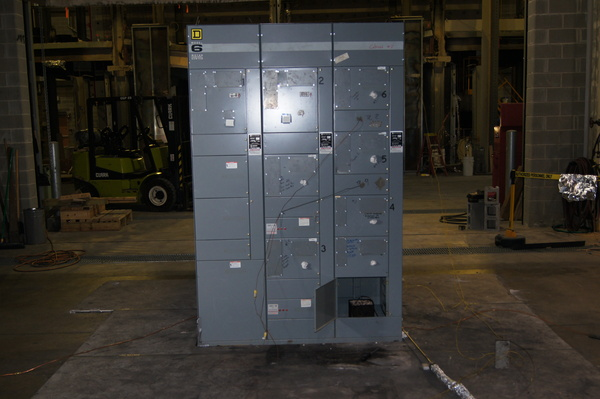
\includegraphics[height=2.0in]{FIGURES/NIST_NRC_OLIVE-Fire/Test_19_photo}
\end{tabular*}
\caption[NIST/NRC OLIVE-Fire enclosure photographs]
{Photographs of the eight electrical enclosures used for the NIST/NRC OLIVE-Fire experiments. The enclosures are numbered 1 through 8 in sequence. Enclosure~\#1 and \#2 (top row) have the same exterior design.}
\label{NIST_NRC_OLIVE_Photos}
\end{figure}

\subsubsection{Modeling Notes}

The simulations are performed with a spatial resolution of 4~cm. The enclosures are modeled simply as rectangular steel boxes with no internal partitions included. Both leakage and vents are modeled in the same way by using the ``localized leakage'' methodology in FDS where the volume flow rate, $\dot{V}$, through a vent or a crack is a function of the pressure difference, $\Delta p$:
\begin{equation}
    \dot{V} = C \, A \, \left( \frac{2 \Delta p}{\rho_0} \right)^{0.5} \left( \frac{\Delta p}{\Delta p_{\rm ref}} \right)^{0.1} \label{leak_eq}
\end{equation}
The discharge coefficient, $C=0.61$, is recommended by the manufacturer of the calibrated fan used for determining the leakage area, $A$. The extra pressure term in the expression represents a weak relationship between the discharge coefficient and the pressure rise. The pressure exponent of 0.6 best fits the leakage data. The reference pressure, $\Delta p_{\rm ref}$, is taken as 1~Pa to maintain unit consistency.


\FloatBarrier

\section{NIST/NRC Parallel Panel Experiments}
\label{NIST_NRC_Parallel_Panels_Description}

As part of a Nuclear Regulatory Commission (NRC) research project to assess fire behavior in electrical enclosures, rate of spread and heat release rate measurements were made on various plastics lining a parallel panel apparatus. The panels were 0.6~m (2~ft) wide, 2.4~m (8~ft) tall, and separated by 0.3~m (1~ft). A 60~kW propane sand burner was positioned at the base of the two panels. Plastics tested to date include PMMA, PVC, and PBT, cut into 6.4~mm (0.25~in) thick panels. A sketch of the apparatus, originally developed by Factory Mutual, is shown in Fig.~\ref{Parallel_Panel_Sketch}.


\section{NIST/NRC Transient Combustibles Experiments}
\label{NIST_NRC_Transient_Combustibles_Description}

In December, 2019 and February, 2020, 40 calorimetry experiments were conducted at the National Fire Research Laboratory at NIST on behalf of the U.S. Nuclear Regulatory Commission. The experiments were conducted under a 6.1~m (20~ft) by 6.1~m hood with a nominal capacity of 3~MW. The full report on the experiments can be found in Ref.~\cite{McGrattan:Multiple_Transients_2020}.

The items burned are described briefly in Fig.~\ref{Items_1}. These consist of commercially available materials constructed mainly of wood and paper. Each item was weighed before and after the experiment on a load cell accurate to 10~g.

The fires were all ignited using one or more 7.5~cm (3~in) segments of approximately 1~cm (0.5~in) diameter cotton rope soaked in approximately 10~mL of acetone. For some items like the wood cribs and pallets, a small amount of shredded craft or ``crinkle'' paper was used to sustain the ignition until steady burning was achieved.

The floor beneath the burning item was protected with a single layer of gypsum board covered by a single layer of concrete board.


\begin{figure}[!t]
\begin{tabular*}{\textwidth}{l@{\extracolsep{\fill}}r}
\parbox[b][2.0in][c]{2.6in}{\sloppy {\bf Box \#1:} Single-wall corrugated box with nominal dimensions 61~cm by 61~cm by 46~cm (24~in by 24~in by 18~in) filled with ``crinkle paper,'' a common packing material made by shredding craft paper. The box alone had a mass of approximately 1.6~kg (3.5~lb), and the box and paper combined had a mass of 8.0~kg (18~lb). The box top flaps were closed, end over end, but not sealed with tape.} &
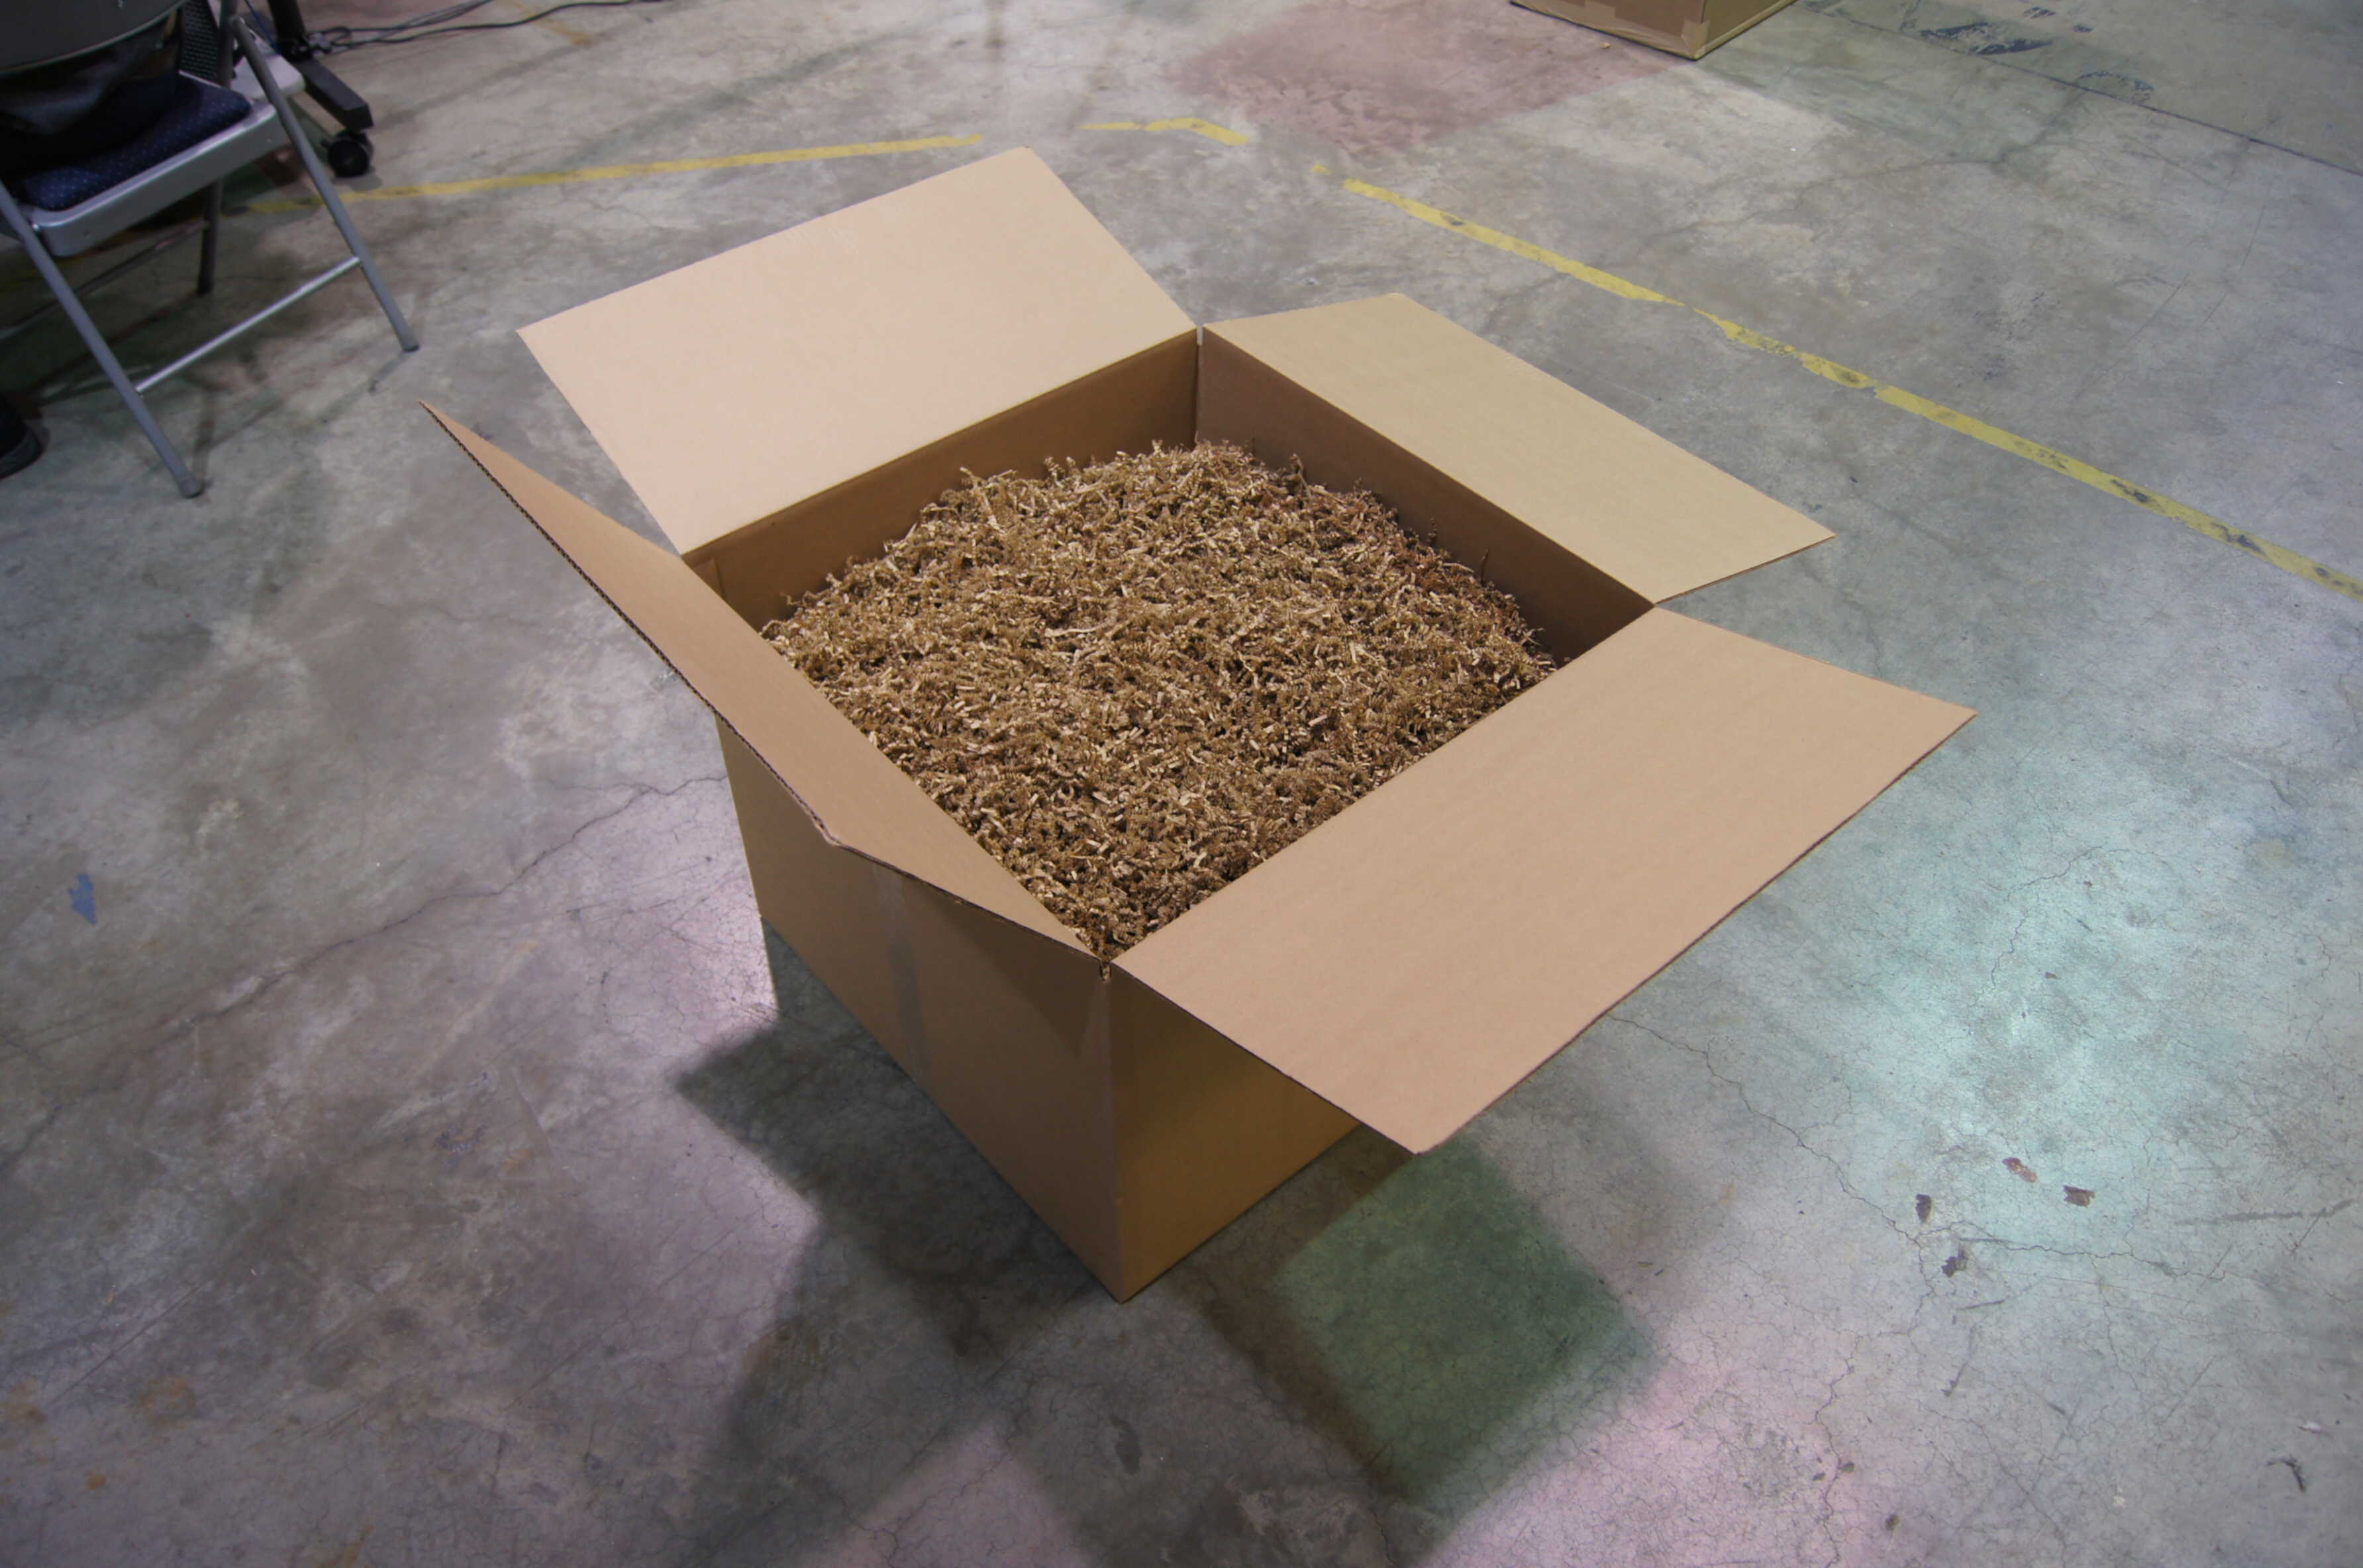
\includegraphics[width=2.9in]{FIGURES/NIST_NRC_Transient_Combustibles/box}  \\
\parbox[b][2.0in][c]{2.6in}{\sloppy {\bf Pallet:} Pine wood pallet with dimensions 122~cm by 102~cm by 12~cm (48~in by 40~in by 4.75~in). Its mass was approximately 16.0~kg (35~lb). Its moisture content was less than 5~\%. Shown at right are two pallets, which were ignited with 1~kg (2.2~lb) of crinkle paper distributed evenly throughout the lower pallet.} &
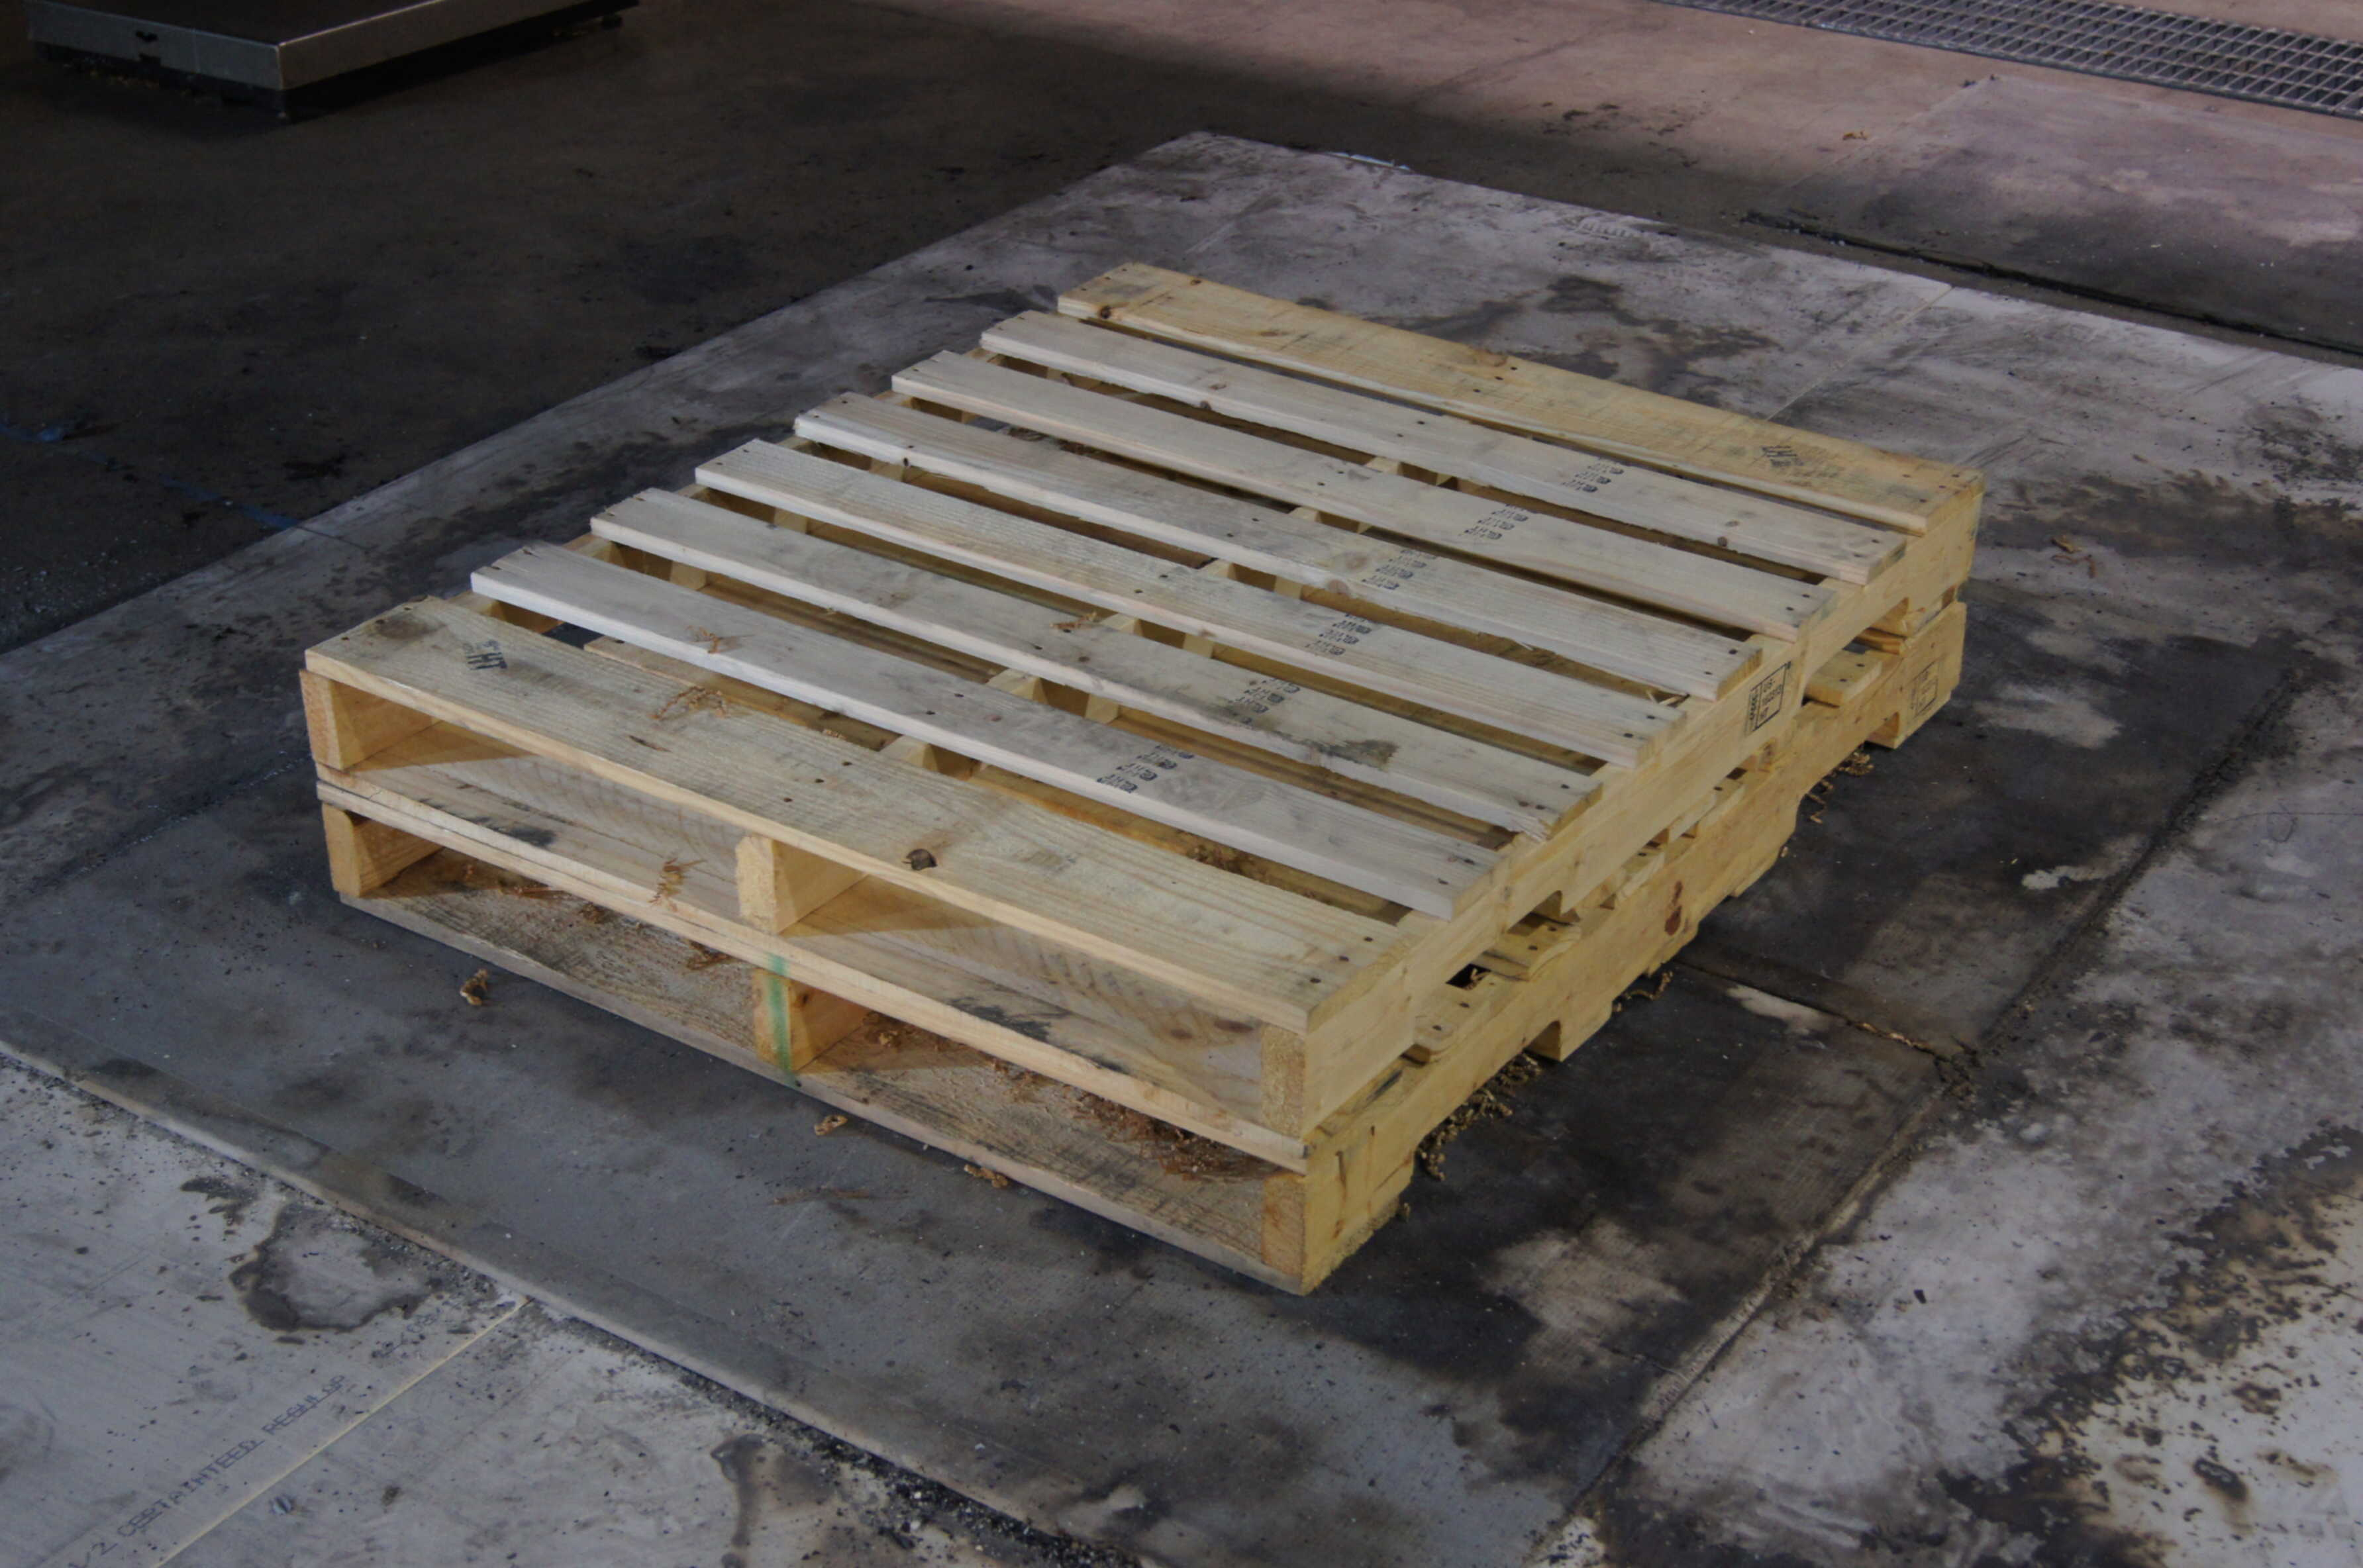
\includegraphics[width=2.9in]{FIGURES/NIST_NRC_Transient_Combustibles/pallet}  \\
\parbox[b][2.0in][c]{2.6in}{\sloppy {\bf Crib:} Pine wood crib with dimensions 56~cm by 56~cm by 46~cm (22~in by 22~in by 18~in) constructed of slats with a cross-section 3.8~cm (1.5~in) square. Its mass was approximately 39~kg (86~lb). Its moisture content was less than 5~\%. It was ignited with 0.75~kg (1.7~lb) of crinkle paper stuffed in the space below the first row of slats.} &
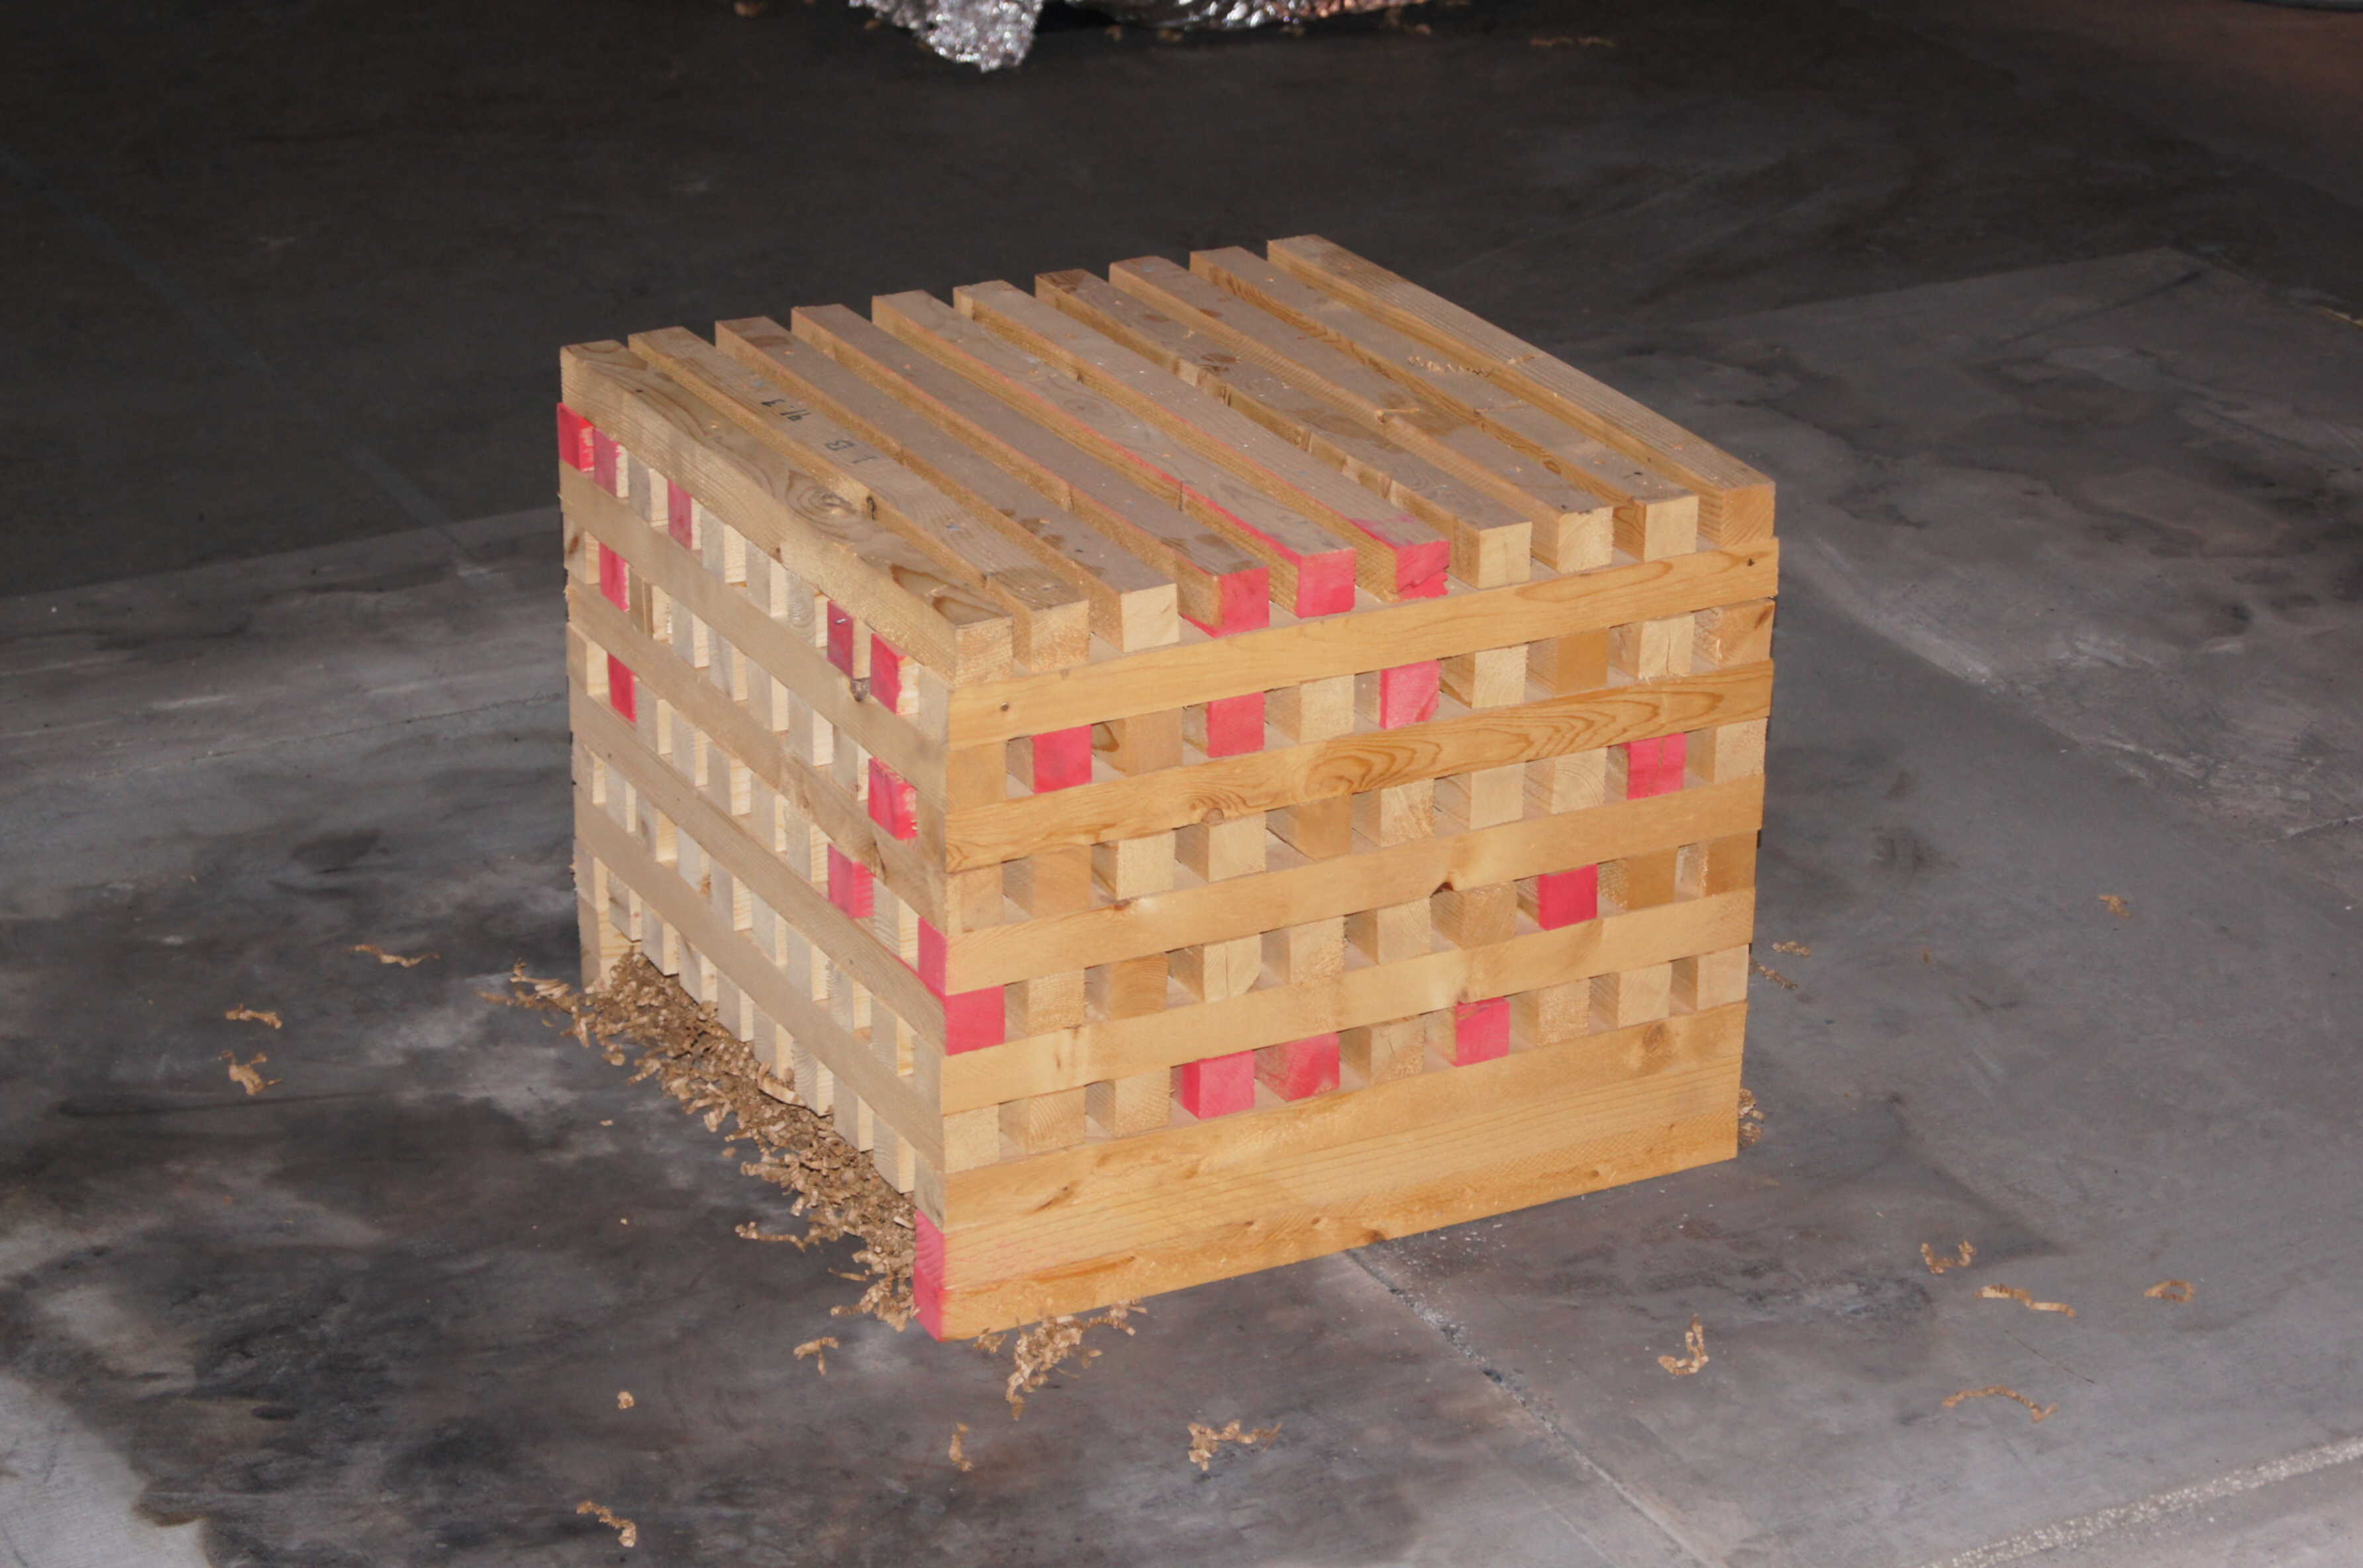
\includegraphics[width=2.9in]{FIGURES/NIST_NRC_Transient_Combustibles/crib}
\end{tabular*}
\caption[Description of test items]{Description of test items.}
\label{Items_1}
\end{figure}

%\begin{figure}[p]
%\begin{tabular*}{\textwidth}{l@{\extracolsep{\fill}}r}
%\parbox[b][2.0in][c]{2.6in}{\sloppy {\bf Box \#2:} Single-wall corrugated box with nominal dimensions 41~cm by 30~cm by 30~cm (16~in by 12~in by 12~in) filled with dry cotton rags. The box alone had a mass of approximately 0.8~kg (1.8~lb), and the box and rags combined had a mass of approximately 4.5~kg (10~lb). The box top was taped shut for the burns.} &
%\includegraphics[width=2.9in]{FIGURES/NIST_NRC_Transient_Combustibles/DSC01463}  \\
%\parbox[b][2.0in][c]{2.6in}{\sloppy {\bf Box \#3:} Single-wall corrugated box with nominal dimensions 53~cm by 53~cm by 53~cm (21~in by 21~in by 21~in) filled with 100 rigid polystyrene cups. The corrugated box and inner liners alone had a mass of approximately 3.5~kg (7.7~lb), and the total combined mass was approximately 7.0~kg (15~lb). The top was taped shut. This item was originally developed by FM Global for use in rack storage commodity testing.} &
%\includegraphics[width=2.9in]{FIGURES/NIST_NRC_Transient_Combustibles/DSC01465} \\
%\parbox[b][2.0in][c]{2.6in}{\sloppy {\bf Tarp:} Lightweight plastic tarp with dimensions 3.0~m by 2.4~m (10~ft by 8~ft) draped across a steel rod. Its mass was approximately 0.8~kg (1.8~lb).} &
%\includegraphics[width=2.9in]{FIGURES/NIST_NRC_Transient_Combustibles/DSC01287} \\
%\parbox[b][2.0in][c]{2.6in}{\sloppy {\bf Bin \#1:} Cylindrical, open-top plastic trash bin approximately 71~cm (28~in) tall with an opening diameter of 51~cm (20~in). Its mass was approximately 2.7~kg (5.9~lb). The bin was half filled with crinkle paper for a combined mass of 5.0~kg (11~lb).} &
%\includegraphics[width=2.9in]{FIGURES/NIST_NRC_Transient_Combustibles/DSC01218}  \\
%\parbox[b][2.0in][c]{2.6in}{\sloppy {\bf Bin \#2:} The same as Bin \#1, but with the rags and cardboard of Box~\#2 mixed in. The total mass was approximately 9.5~kg (21~lb).} &
%\includegraphics[width=2.9in]{FIGURES/NIST_NRC_Transient_Combustibles/DSC01358}
%\end{tabular*}
%\caption[Description of test items (cont.)]{Description of test items (cont.)}
%\label{Items_2}
%\end{figure}

The heats of combustion and product yields of the various items burned are given in Table~\ref{Item_Yields}. These values are derived from the measured initial and final mass, and an assumed value of 13.61~MJ/kg for the energy released per unit mass of oxygen consumed.

\begin{table}[h]
\caption[Average heat and product yields of the various test items]{Average heat and product yields of the various test items.}
\centering
\begin{tabular}{|c|c|c|c|c|c|}
\hline
Item        & $\Delta H$ (MJ/kg)  & CO Yield           & CO$_2$ Yield   & Soot Yield          & Residue Yield               \\ \hline \hline
Box \#1     & $14.8\pm0.5$        & $0.039\pm0.001$    & $1.48\pm0.05$  & $0.0014\pm0.0003$   & $0.031\pm0.016$               \\ \hline
%Box \#2     & $13.8\pm0.5$        & $0.066\pm0.003$    & $1.33\pm0.05$  & $0.0042\pm0.0019$   & $0.035\pm0.020$               \\ \hline
%Box \#3     & $25.4\pm1.5$        & $0.055\pm0.002$    & $2.13\pm0.08$  & $0.0976\pm0.014  $  & $0.003\pm0.002$               \\ \hline
Pallet      & $17.2\pm0.5$        & $0.031\pm0.001$    & $1.66\pm0.06$  & $0.0033\pm0.0006$   & $0.059\pm0.024$               \\ \hline
Crib        & $16.7\pm0.5$        & $0.023\pm0.001$    & $1.63\pm0.06$  & $0.0020\pm0.0003$   & $0.053\pm0.034$               \\ \hline
%Bin \#1     & $27.6\pm1.7$        & $0.021\pm0.004$    & $2.18\pm0.08$  & $0.0153\pm0.0027$   & $0.090\pm0.040$               \\ \hline
%Bin \#2     & $20.8\pm1.2$        & $0.031\pm0.001$    & $1.80\pm0.07$  & $0.0099\pm0.0029$   & $0.040\pm0.020$               \\ \hline
\end{tabular}
\label{Item_Yields}
\end{table}

\subsubsection{Modeling Notes}

The combustible items are modeled as collections of Lagrangian particles that undergo a three-step decomposition process consisting of moisture evaporation, pyrolysis, and char oxidation. The moisture content, $M$, of the conditioned materials was less than the 0.05 lower limit of the moisture meter, and this value is used in the calculations.

In the model, all of the wood and paper materials are assumed to be made up of cellulose, C$_6$H$_{10}$O$_5$, with a net heat of combustion of 16.12~MJ/kg~\cite{SFPE}. It is also assumed that the materials have a char yield of 20~\%, meaning that 20~\% of the dry mass is converted into char that undergoes an exothermic oxidation reaction generating 32.12~MJ/kg of char consumed. The decomposition reactions are as follows:

\vspace{\baselineskip}

\noindent 1. Endothermic moisture evaporation
\be
 {\rm Wet\ Vegetation} \rightarrow \nu_{\rm H_2O} \, {\rm H_2O} + (1-\nu_{\rm H_2O}) \, {\rm Dry\ Vegetation} \quad ; \quad \nu_{\rm H_2O} = \frac{M}{1+M}
\ee
\noindent 2. Endothermic pyrolysis of dry vegetation
\be
 {\rm Dry\ Vegetation} \rightarrow 0.2 \, {\rm Char} + 0.8 \, \hbox{C}_{3.3}\hbox{H}_{10}\hbox{O}_5
\ee
\noindent 3. Exothermic char oxidation
\be
 \label{char_reaction}
 {\rm Char} + 1.65 \, {\rm O_2} \rightarrow 2.4 \, {\rm CO_2} + 0.25 \, {\rm Ash}
\ee
Note that the fuel gas is taken as cellulose with 20~\% of its molecular mass decreased to account for the residual char, which is assumed to be pure carbon. The heat of combustion of this modified fuel gas is 12120~MJ/kg. The yield of residual Ash is based on the measured residual mass.

The crinkle paper is assumed to consist of 3~cm long, 4~mm wide strips with a surface area to volume ratio of 10000~m$^{-1}$ (approximately 0.2~mm thick). The length and width are important only in defining the mass and volume of each particle. The thermal and kinetic properties of the paper are assumed to be similar to those of corrugated cardboard given in Table~\ref{Properties_Cardboard}. The cardboard that makes up the box that holds the crinkle paper has a mass of 0.62~kg/m$^2$ and the box itself has a mass of 1.6~kg. The corrugated paper has an assumed dry density of 350~kg/m$^3$, yielding an effective thickness of 1.8~mm. In the model, the box does not undergo char oxidation but rather ``burns away'' to expose the crinkle paper inside.

The wood crib is made up of 104 56~cm (22~in) long, 3.8~cm (1.5~in) square interlacing pine wood strips. The particles used to model the crib are assumed to be cylindrical in shape but with a surface area to volume ratio of 69~m$^{-1}$ based on a direct measurement of the actual crib geometry. The dry density of the wood has been measured to be 463~kg/m$^3$, its peak pyrolysis temperature is taken to be 320~$^\circ$C~\cite{Fraga:2020}, its char yield assumed to be 20~\%, and its heat of reaction is taken to be 418~kJ/kg~\cite{Morvan:CF2001}. Other property values are based on the default vegetation pyrolysis model described in the FDS User's Guide.

The pine wood pallets are constructed of 1.6~cm (5/8~in) thick planks and modeled as a collection of flat particles with a thickness of 8~mm and the same thermal and kinetic properties as the cribs, except that the wood making up the pallets has a dry density of 414~kg/m$^3$.

The drag per unit volume exerted by the particles is given by
\be
   \mathbf{f} = \frac{\rho}{2} C_{\rm d} \, \kappa \, \bu |\bu|   \quad ; \quad \kappa = C_{\rm s} \sigma \beta
\ee
where $\rho$ is the gas density, $C_{\rm d}$ is a drag coefficient, $\bu$ is the local velocity vector, $C_{\rm s}$ is a shape factor, $\sigma$ is the surface area to volume ratio, and $\beta$ is the packing ratio; that is the ratio of particle volume to cell volume. The shape factor is taken as 0.25 for all particle types. The packing ratio is determined by the measured mass of the item and the volume it occupies. The drag coefficient for the wood crib is 65, a value obtained by simulating a finely-resolved wood crib in a wind tunnel and calibrating the drag of the equivalent ``crib particles'' accordingly. The drag coefficient of the crinkle paper is taken as 1, and that of the pallet is taken as 3. These are only order of magnitude estimates and have not been verified.


\section{NIST Pool Fire Experiments}
\label{NIST_Pool_Fires_Description}

The NIST Pool Fire Experiments include temperature, species concentration, velocity, and heat flux measurements of 30~cm and 100~cm diameter circular liquid fuel fires, and 37~cm gaseous burner fires.

The 30~cm burner is 15~cm deep and has a wall thickness of 1.6~mm. The burner is fitted with legs such that the burner rim is positioned 30~cm above the floor. The bottom of the burner is maintained at a constant temperature by flowing tap water (nominally 20~$^\circ$C) through a 3~cm section on the bottom of the fuel pan. The dimensions of the circular burner are similar to Weckman's methanol experiment described in Section~\ref{Waterloo_Methanol_Description}.

The 100~cm burner is also 15~cm deep, has a wall thickness of 1.6~mm, and is water-cooled.

The 37~cm burner is actually 38~cm in diameter with an effective diameter of 37~cm. It is water cooled, and the surface temperature is maintained at approximately 40~$^\circ$C.  The measured fuel flow rate for the methane fire was 0.69~g/s and its estimated HRR was 34.5~kW. The heat release rates of the two propane fires were 20~kW and 34~kW.

Details and references with regard to the plume temperature measurements are given in Section~\ref{NIST_Pool_Fires_Plume_Temps}. Details on the heat flux measurements are given in Section~\ref{NIST_Pool_Fires_Heat_Flux_Results}. Details on the gas species measurements is given in Section~\ref{sec:NIST_Pool_Fires}. Details on the velocity measuremnts is given in Section~\ref{NIST_Pool_Fires_Velocity}.


\subsubsection{Modeling Notes}

The 30~cm pool fires are modeled at three different grid resolutions---2~cm, 1~cm, and 0.5~cm. The 100~cm pool fires are modeled at 4~cm, 2~cm, and 1~cm resolution. The mass loss rate of the fuel is specified.

A two-step reaction mechanism is implemented. In the first reaction, fuel is converted to CO, soot, H$_2$, and H$_2$O. In the second reaction, the CO, soot, and H$_2$ are converted to CO$_2$ and H$_2$O. Both reactions employ fast kinetics, but proceed in series, not in parallel. The relative amounts of CO, soot, and H$_2$ produced in the first step are still subjects of study, and for the moment have been estimated based on measured results. The fractions of carbon atoms converted to CO in the first step are as follows---0.85 for acetone; 0.95 for ethanol; 0.97 for methane; 1.0 for methanol; 0.85 for propane. For all fuels, one half of the hydrogen atoms are converted to H$_2$ in the first step.

The radiative fractions are specified based on measured values---0.31 for acetone; 0.26 for ethanol; 0.15 for methane; 0.21 for 1~m methanol; 0.22 for 30~cm methanol; 0.22 for propane.


\section{NIST Smoke Alarm Experiments}
\label{NIST_Smoke_Alarm_Description}

A series of experiments was conducted by NIST to measure the activation time of ionization and photoelectric smoke alarms in a residential setting~\cite{Bukowski:1}. Tests were conducted in actual homes with representative sizes and floor plans, utilized actual furnishings and household items for fire sources, and tested actual smoke alarms sold in retail stores at that time. Thirty-six tests were conducted in two homes; 27 in a single-story manufactured home, and 8 in a two-story home. Eight experiments that were conducted in the single-story manufactured home were selected for model validation. Only tests that used a flaming ignition source with a couch or mattress fuel package were considered; the cooking oil fires and tests that used a smoldering ignition source were not considered. The flaming ignition tests used a moderate flame source to quickly ignite the fuel package.

The primary partitioning of the single-story floor plan consisted of three bedrooms, one full bathroom, one kitchen/dining area, one living room, and two hallways (see Fig.~\ref{NIST_Smoke_Alarms_Drawing}). For testing, the doors to Bedroom~3 and the bathroom were always closed. The ceiling was peaked on the long axis, reaching a height of 2.4~m. The outside walls were approximately 2.1~m in height. The slope of the ceiling was approximately 8.4$^\circ$. Groups of smoke alarms were located in the room of fire origin, at least one bedroom, and in a central location. Five stations (Station A through Station E) containing smoke alarm\footnote{Note that, in the FDS Guides, smoke detectors and smoke alarms are collectively referred to as smoke detectors because the same smoke detection algorithm is used to predict activation of either type of device.} arrays were mounted parallel to the ceiling.

Although a load cell was used in the experiments to measure the mass loss rate of the fuel package, the mass loss data were not reliable enough to reconstruct the HRR curves for each test. Instead, the HRR curves were determined by approximating the fire growth using a $t$-squared ramp, as in Eq.~(\ref{eq:t_squared}). The parameters for the $t$-squared ramp were calibrated in FDS by using the temperature measured at the highest thermocouple in the tree (2~cm below the ceiling) in the fire room.
\be
\dot Q = \dot Q_0 \left( \frac{t}{\tau} \right)^2
\label{eq:t_squared}
\ee
A time offset was used to align the predicted ceiling thermocouple temperatures with the measured temperatures. This offset is reported as the time at which the $t$-squared ramp begins. The t-squared calibration parameters and time offsets for the HRR ramps are shown in Table~\ref{tab:NIST_Smoke_Alarms_Summary}. Additionally, the ignition source had a small effect on the measured ceiling thermocouple temperatures. Therefore, the size of the ignition source was approximated as either 3~kW or 7~kW, and the time offset of the ignition source was also calibrated by using the measured ceiling thermocouple temperatures. The resulting HRR curve was input into FDS as a fire ramp. A summary of the eight tests selected for model validation is shown in Table~\ref{tab:NIST_Smoke_Alarms_Summary}.

\begin{table}[h!]
\caption[Summary of NIST Smoke Alarm Experiments selected for model validation]{Summary of NIST Smoke Alarm Experiments selected for model validation.}
\begin{center}
\begin{tabular}{|c|c|c|c|c|c|}
\hline
Test No.  &  Fire Source  &  Fire Location  &  $\dot Q_0$ (kW)  &  $\tau$ (s)  &  Time Offset (s)  \\ \hline \hline
SDC02     &  Chair        &  Living Room    &  150              &  180         &  20               \\ \hline
SDC05     &  Mattress     &  Bedroom        &  200              &  180         &  20               \\ \hline
SDC07     &  Mattress     &  Bedroom        &  350              &  180         &  50               \\ \hline
SDC10     &  Chair        &  Living Room    &  150              &  180         &  40               \\ \hline
SDC33     &  Chair        &  Living Room    &  100              &  180         &  10               \\ \hline
SDC35     &  Chair        &  Living Room    &  100              &  180         &  10               \\ \hline
SDC38     &  Mattress     &  Bedroom        &  120              &  180         &  25               \\ \hline
SDC39     &  Mattress     &  Bedroom        &  200              &  180         &  25               \\ \hline
\end{tabular}
\end{center}
\label{tab:NIST_Smoke_Alarms_Summary}
\end{table}

\begin{figure}[p]
\includegraphics[width=\textwidth]{FIGURES/NIST_Smoke_Alarms/Manufactured_Home_Drawing}
\caption[Geometry of the manufactured home from the NIST Smoke Alarm Experiments]{Geometry of the manufactured home from the NIST Smoke Alarm Experiments.}
\label{NIST_Smoke_Alarms_Drawing}
\end{figure}

\FloatBarrier

\section{NIST Soot Deposition Gauge}
\label{NIST_SDG_Description}

A series of tests were performed as part of an effort to develop a gauge capable of making real time measurements of soot deposition \cite{NIST_SDG}. The test apparatus consisted of a hot plate and cold plate measuring 8 cm wide by 41~cm long and separated by 1~cm. The hot plate was electrically heated and the cold plate was water cooled. A laminar diffusion flame burner using propene as the fuel was used to generate soot. A portion of the effluent from the burner was sent through the test apparatus. In addition to tests using the new gauge, a series of gravimetric tests were performed using 47~mm diameter pieces of aluminum foil attached to the cold plate in four locations. Tests with the aluminum foil used nominal flowrates of 2.5, 5.0, and 10.0 SLPM and nominal temperature differences of 100~$^{\circ}$C and 200~$^{\circ}$C. The test channel was mounted vertically to avoid gravitational settling and with the laminar flow speeds the device essentially creates only thermophoretic deposition. Four replicate tests were performed for the 2.5 and 5.0 SLPM flowrates and three for the 10.0 SLPM flowrate. A summary of the 22 tests modeled is given in the table below.

\begin{table}[h!]
	\caption{Experiment Details for Gravimetric Measurements of Soot Deposition}
	\begin{center}
		\begin{tabular}{|c|c|c|c|}
			\hline
		Test no. & Flow Speed & $\Delta$T & Inlet Soot Conc.  \\
		         & (SLPM)     & (K)       & (mg/m$^3$)        \\ \hline \hline
		1        & 2.5        &  94       &  67.6             \\ \hline
		2        & 2.5        &  94       &  69.2             \\ \hline
		3        & 2.5        &  96       &  64.2             \\ \hline
		4        & 2.5        &  96       &  64.2             \\ \hline
		5        & 5.0        &  96       &  65.5             \\ \hline
		6        & 5.0        &  95       &  62.7             \\ \hline
		7        & 5.0        &  92       &  61.9             \\ \hline
		8        & 5.0        &  94       &  68.4             \\ \hline
		9        & 10.0       &  97       &  25.9             \\ \hline
		10       & 10.0       &  98       &  27.4             \\ \hline
		11       & 10.0       &  99       &  25.5             \\ \hline
		12       & 2.5        &  187      &  60.2             \\ \hline
		13       & 2.5        &  190      &  61.5             \\ \hline
		14       & 2.5        &  189      &  64.2             \\ \hline
		15       & 2.5        &  187      &  59.1             \\ \hline
		16       & 5.0        &  188      &  59.7             \\ \hline
		17       & 5.0        &  186      &  58.5             \\ \hline
		18       & 5.0        &  187      &  60.7             \\ \hline
		19       & 5.0        &  187      &  55.5             \\ \hline
		20       & 10.0       &  191      &  23.5             \\ \hline
		22       & 10.0       &  188      &  24.4             \\ \hline
		21       & 10.0       &  189      &  22.6             \\ \hline
		\end{tabular}
	\end{center}
	\label{tab:NIST_SDG}
\end{table}


\section{NIST Structure Separation Experiments}
\label{NIST_Structure_Separation_Description}

Maranghides et al.~\cite{Maranghides:TN2161,Maranghides:TN2235} have developed a series of tests designed to understand safe structure separation distances for sheds, fences, and other combustible materials, with and without wind, in the wildland-urban interface (WUI).

\subsubsection{Verification Tests}

Prior to modeling heat fluxes to surfaces with attached flames or modeling ignition of siding material, a relatively simple test was carried out to record heat fluxes from a know fire source to targets in the proximity to the flame.  The 8 MW NFRL calibration burner \cite{Bryant:NISTSP1007} (see Fig.~\ref{NFRL_8MW_calibration_burner}) is positioned on a raised platform under the medium scale hood in NFRL.  Three heat flux gauge towers are positioned 1, 2, and 3 m from the burner edge (or 2, 3, and 4 m from the burner center).  Figure~\ref{NIST_SSE_Verification_Setup} shows a photograph from \cite{Maranghides:TN2235} (courtesy Matt Hoehler).

\begin{figure}[h]
\centering
\includegraphics[width=.75\textwidth]{../../../cad/NIST_Calibration_Burners/NIST_8MW_assembly_drawing}
\caption[NFRL 8 MW calibration burner assembly drawing]{NFRL 8 MW calibration burner assembly drawing produced by NIST SURF student Louis Serrano Torres.  Units in inches.}
\label{NFRL_8MW_calibration_burner}
\end{figure}

\begin{figure}[h]
\centering
\includegraphics[width=.75\textwidth]{FIGURES/NIST_Structure_Separation/SSE_Verification_Exp_Setup}
\caption[Structure Separation Verification setup]{Structure Separation Verification setup showing natural gas burner and heat flux gauge positions.}
\label{NIST_SSE_Verification_Setup}
\end{figure}

\subsubsection{Modeling Notes}

The burner is roughly 1 m $\times$ 1.5 m with 802 fuel ports 1/8th inch in diameter (see Fig.~\ref{NFRL_8MW_calibration_burner}).  The FDS model of the burner is built from particles (see Fig below).  Each particle has a radius set to give a spherical area equivalent to a 1/8th inch diameter fuel port.  The time ramp in the FDS simulation is compressed by a factor of 10.  The ``gauge heat flux'' is recorded in an orientation pointing toward the burner ($+x$ direction).  The burner flow baffle plates are made from thin {\ct OBST}.  Fictitious manifolds are made from thickened {\ct OBST}.  The number of radiation angles in increased to 400.  The radiation path length is set to 2 m.  Ambient conditions are taken from historical weather data for the day of the experiment.  The natural gas composition is taken from NFRL records on the day.  A radiant fraction of 0.25 is prescribed, which is both consistent with a methane flame with additional ethane and the heat flux data farthest from the fire source under the assumption of a point source model.  The burner has a $D^*$ of approximately 2.2.  As a baseline, a grid resolution of 5 cm provides a $D^*/\Delta x = 44$.  Reasonably high resolution may be necessary if near-flame heat flux values are of interest.  However, we also provide FDS results for 10 cm resolution.

\begin{figure}[h]
\centering
\includegraphics[width=.5\textwidth]{FIGURES/NIST_Structure_Separation/nfrl_burner_particles}
\caption[FDS particle model of NFRL 8 MW burner]{Image of the FDS particle model for the 8 MW NFRL burner.}
\label{FDS_NFRL_8MW_particle_burner}
\end{figure}


\section{NIST Vent Study}
\label{NIST_Vent_Description}

A series of 15 reduced-scale enclosure experiments were conducted during the summer of 2017 by Summer Undergraduate Research Fellows (SURF) Fateema Farzana and Cory Schovanec. There is no test report or paper describing these experiments; only what is included here.

\subsubsection{Enclosure Geometry}
\label{Enclosure_Geometry}

A drawing of the enclosure is given in Fig.~\ref{NIST_Vent_Study_Drawing}. The enclosure consisted of two compartments stacked one on top of the other. The interior lateral dimensions of each compartment were 119~cm by 121~cm. The height of the lower compartment was 59~cm, and the upper was 61~cm. The enclosure was located within a vented laboratory space that was approximately 3~m by 3~m by 2.8~m high. The floor of this space was tiled, but a single sheet of gypsum board served as the lower floor of the test enclosure.

The front door was open in all experiments. For some portion of some of the experiments, the second floor was completely sealed. The leakage area was approximately 18~cm$^2$, measured at an over-pressure of 25~Pa.

\begin{figure}[p]
\includegraphics[width=\textwidth]{FIGURES/NIST_Vent_Study/Latex_Drawing_Plan}
\includegraphics[width=\textwidth]{FIGURES/NIST_Vent_Study/Latex_Drawing_Front}
\caption[Geometry of the compartment from the NIST Vent Study]{Geometry of the compartment from the NIST Vent Study}
\label{NIST_Vent_Study_Drawing}
\end{figure}

\subsubsection{Material Properties}

The walls, ceiling and floor of each compartment was 1.6~cm (5/8~in) Type~X gypsum board. Wood studs formed the exterior frame. Thermo-physical properties of the gypsum board were taken from in Ref.~\cite{Manzello:SiF08} and manufacturer literature. It was assumed that the specific heat was 1.089~kJ/(kg $\cdot$ K), thermal conductivity 0.15~W/m/K, and density 673~kg/m$^3$.  Additionally, a  layer of kaowool, shown in Fig.~\ref{NIST_Vent_Study_Drawing} was used to seal the gap between the removable roof and the second story walls. Aluminum tape was used to seal all other seams.

\subsubsection{Burner}

For all experiments, a 10~cm square propane burner fueled at a rate of 1.65~L/min generated a 2.5~kW fire according to the following calculation:
\be
   1.65 \frac{\rm L}{\rm min} \times \frac{1}{60} \frac{\rm min}{\rm s} \times \frac{1}{1000} \frac{{\rm m}^3}{\rm L} \times 1.967 \, \frac{\rm kg}{{\rm m}^3} \times 46,300 \, \frac{\rm kJ}{\rm kg} = 2.50 \; {\rm kW}
\label{Conversion_Equation}
\ee
Note that the mass flow controller (Sierra Instruments SmartTrak~50) assumed standard conditions to be 0~$^\circ$C and 101325~Pa. For Tests~13-15, a Dwyer flow meter was used in place of the mass flow controller. The flow meter had a flow range of 4~L/min air.

\subsubsection{Thermocouples}

Eight Type-K thermocouples were inserted at each level to measure the vertical temperature profile. The thermocouples formed a vertical array at 84~cm from the left wall of the enclosure, and 17~cm from the front wall. TC-1 was defined as the uppermost thermocouple, with heights defined as the vertical distance from the compartment specific floor.

\begin{table}[h!]
\caption{Heights of the thermocouples above the floor of each level of the enclosure}
\begin{center}
\begin{tabular}{|c|c|c|c|c|c|c|c|c|c|c|c|c|c|c|c|c|}
\hline
Floor 2 TC's   & 1& 2& 3 & 4& 5& 6& 7&8\\ \hline
Height (cm) & 56.5& 50.8& 45.5& 41.0& 36.0& 29.8& 19.8& 10.5\\ \hline
Floor 1 TC's & 9&10&11&12&13&14&15&16\\ \hline
Height (cm) &51.8&47.0&40.64&35.6&30.48&25.7& 16.5&7.0\\ \hline


\end{tabular}
\end{center}
\label{Tab.TC}
\end{table}

\subsubsection{Test Procedure}

Each experiment lasted 100~min with a 5~min cool down period. Table~\ref{tab:NIST_Vent_Study} indicates the times when vents and windows were opened after the start of each experiment. For Test No. 1-4, two trials were performed. In each case, the difference in temperature remained within 3 percent, a difference of less than 1~$^\circ$C. For this reason, no further replicates were conducted.

\begin{table}[h!]
\caption{Vent State by Experiment: Time Opened}
\begin{center}
\begin{tabular}{|c|c|c|c|c|c|c|c|c|c|}
\hline
Test & Front    & Left    & Right     & Left     & Right   & Left         & Right        & Right   & Roof    \\
No.  & Window   & Window  & Window    & Vent     & Vent    & Vent Area    & Vent Area    & Vent    & Vent    \\
     & (min)    & (min)   & (min)     & (min)    & (min)   & (cm$^2$)     & (cm$^2$)     & Shape   & (min)   \\ \hline \hline
1    & 0        &  0      &  0        &  Closed  &  0      &  0           &  100         &  Square & Closed  \\ \hline
2    & 0        &  0      &  0        &  Closed  &  20     &  0           &  100         &  Square & Closed  \\ \hline
3    & 60       &  40     &  Closed   &  Closed  &  20     &  0           &  100         &  Square & Closed  \\ \hline
4    & 0        &  0      &  0        &  Closed  &  0      &  0           & 400          &  Square & Closed  \\ \hline
5    & 0        &  0      &  0        &  Closed  &  20     &  0           &  400         &  Square & Closed  \\ \hline
6    & 60       &  40     &  Closed   &  Closed  &  20     &  0           &  400         &  Square & Closed  \\ \hline
7    &  0       &  0      &  0        &  0       &  0      &  100         &  400         &  Square & Closed  \\ \hline
8    &  0       &  0      &  0        &  20      &  40     &  100         &  400         &  Square & Closed  \\ \hline
9    &  80      &  60     &  Closed   &  20      &  40     &  100         &  400         &  Square & Closed  \\ \hline
10   &  0       &  0      &  0        &  Closed  &  0      &  0           &  100         & Circle  & Closed  \\ \hline
11   &  0       &  0      &  0        &  Closed  &  20     &  0           &  100         & Circle  & Closed  \\ \hline
12   &  60      &  40     &  Closed   &  Closed  &  20     &  0           &  100         & Circle  & Closed  \\ \hline
13   &  0       &  0      &  0        &  0       &  0      &  100         &  400         &  Square & 0       \\ \hline
14   &  0       &  0      &  0        &  20      &  40     &  100         &  400         &  Square & 60      \\ \hline
15   &  Closed  & Closed  &  Closed   &  20      &  40     &  100         &  400         &  Square & 60      \\ \hline
\end{tabular}
\end{center}
\label{tab:NIST_Vent_Study}
\end{table}


\FloatBarrier

\section{NRCC Facade Heat Flux Measurements}
\label{NRCC_Facade_Description}

A series of experiments was conducted by the Fire Research Section of the Institute for Research in Construction, National Research Council of Canada (NRCC), to measure the heat flux to a mock exterior building facade due to a fire within a compartment~\cite{Oleszkiewicz:ASME,Oleszkiewicz:FireTech}. The experiments selected for model validation were conducted using a series of propane line burners within a compartment whose interior dimensions were 5.95~m wide, 4.4~m deep, and 2.75~m high (see Fig.~\ref{NRCC_Facade_Drawing}). There were five different door/window sizes:
\begin{enumerate}
\item 0.94 m by 2.00 m high
\item 0.94 m by 2.70 m high (door)
\item 2.60 m by 1.37 m high (shown in Fig.~\ref{NRCC_Facade_Drawing})
\item 2.60 m by 2.00 m high
\item 2.60 m by 2.70 m high (door)
\end{enumerate}
There were four fire sizes: 5.5~MW, 6.9~MW, 8.6~MW, and 10.3~MW. In all, 19 experiments were conducted, with the exception of the 10.3~MW fire with Window~1. In each experiment, heat flux measurements were made 0.5~m, 1.5~m, 2.5~m, and 3.5~m above the top of the door/window.

\begin{figure}[p]
\includegraphics[width=\textwidth]{FIGURES/NRCC_Facade/NRCC_Facade}
\caption[Geometry of the NRCC Facade Experiments]{Geometry of the NRCC Facade Experiments.}
\label{NRCC_Facade_Drawing}
\end{figure}


\section{NRCC Smoke Tower Experiments}
\label{NRCC_Smoke_Tower_Description}

In 2006 and 2007, the National Research Council of Canada (NRCC) conducted 10 fire experiments in a 10 story experimental facility in Almonte, Ontario to study smoke movement through the stair shaft to the upper floors of the building. Four of these experiments utilized actual commodities as fuel, and six utilized a propane burner. Four of the six propane fires were intended to reproduce the heat release of the commodity fires, and these experiments (BK-R, CMP-R, CLC-I-R, and CLC-II-R) have been chosen for this guide. Details of the experiments are included in a master's thesis and paper by Yan Wang~\cite{Wang:Thesis,Wang:FT2011}. A description of FDS simulations of the propane experiments not included in this guide is given by Hadjisophocleous and Jia~\cite{Hadjisophocleous:FT2009}. The analysis of the propane burner experiments discussed in this guide are based on the work of Paul Tyson at Ulster University as part of his master's thesis~\cite{Tyson:Thesis}.

\begin{figure}[p]
\includegraphics[width=\textwidth]{FIGURES/NRCC_Smoke_Tower/NRCC_Smoke_Tower}
\caption[Geometry of the NRCC Smoke Tower Experiments]{Geometry of the NRCC Smoke Tower Experiments.}
\label{NRCC_Smoke_Tower_Drawing}
\end{figure}

The tower was designed as a test bed for the center core of a high-rise building. It includes a compartment and corridor on each floor, a stair shaft, elevator shaft and service shafts~\cite{Achakji:1987}. Figure~\ref{NRCC_Smoke_Tower_Drawing} displays the geometry of the building as modeled in FDS. All walls and floor slabs are taken to be 0.2~m thick. The first two floors are 3.4~m high, slab to slab. The upper eight floors are 2.4~m, slab to slab. The propane burner was located on the second floor and the smoke flowed through open doors to the stair vestibule and stair shaft itself. In the four experiments considered in this guide, the stair shaft was open on the fourth, sixth, eighth, and tenth floors. The other floors were closed off to the stair shaft. The ventilation system was turned off. A single door was opened on the first floor, and there were no other openings to the outside save natural building leakage. The referenced documents do not explicitly include estimates of leakage areas, but for the sake of modeling, the leakage for each floor was concentrated at a single 1.5~m by 1.5~m exterior window. The leakage area was specified based on an estimate of a ``loose'' building exterior in NFPA~92~\cite{NFPA_92}. This is a very important consideration in modeling because it determines the extent to which the smoke rising up the stair shaft encounters an opposing downward flow.

Thermocouples and gas analyzers were placed at various locations to measure temperature and O$_2$, CO$_2$ and CO concentrations. A vertical array of TCs was located in the fire compartment and the doorway leading into the stair shaft on the second floor. TCs were also placed at each floor in the stair shaft. The gas analyzers were located in the stair shaft at the second floor, just outside the door to the fire compartment.



%\section{NRL Confined Space Experiments}
%
%The U.S. Naval Research Laboratory (NRL) performed a multi-year series of experiments inside of a four level,
%23 compartment test facility with 20 doors and ceiling vents whose exterior boundaries were airtight~\cite{Confined_JFPE} ~\cite{Confined_DTIC}.
%Three HVAC systems were installed in the facility: a supply air system that takes suction from a fan room and discharges the air to the each of the compartments,
%an exhaust system that takes suction from each of the compartments and discharges it to the fan room, and a smoke control control system that takes suction from an upper
%level compartment and discharges it to the ambient (see Figure~\ref{confined_HVAC}).
%A second set of HVAC ducts directly connected the second level with the fourth level (see Figure~\ref{confined_bypass}).
%
%\begin{figure}[ht]
%\begin{center}
%%\includegraphics[width=5.in]{FIGURES/NRL_Confined_Space/confined_space_hvac_layout}
%\end{center}
%\caption{Confined space HVAC system layouts.}
%\label{confined_HVAC}
%\end{figure}
%
%\begin{figure}[ht]
%\begin{center}
%%\includegraphics[width=5.in]{FIGURES/NRL_Confined_Space/confined_space_bypass}
%\end{center}
%\caption{Confined space bypass ducts.}
%\label{confined_bypass}
%\end{figure}
%
%The test facility was instrumented with gas thermocouples, surface thermocouples, optical density meters, gas sampling lines (CO$_2$, CO, and O$_2$),
%and velocity probes in a small number of doors, vents, and HVAC ducts.  Test variables included the number of opened doors and hatches, the number of vent openings to the ambient,
%the fire location, the fire size, and the operation of the HVAC systems.  All the fires were marine diesel pool fires.
%
%\FloatBarrier


\section{NRL/HAI Wall Heat Flux Measurements}
\label{NRL_HAI_Description}

Back, Beyler, DiNenno and Tatem~\cite{Back:IAFSS4} measured the heat flux from 9 different sized propane fires set up against a wall composed
of gypsum board. The experiments were sponsored by the Naval Research Laboratory and conducted by Hughes Associates, Inc., of Baltimore, Maryland. The
square sand burner ranged in size from 0.28~m to 0.70~m, and the fires ranged in size from 50~kW to 520~kW.


\section{Phoenix LNG Fires}
\label{Phoenix_LNG_Fires_Description}

In 2009, Sandia National Laboratories conducted two large-scale LNG pool fire experiments in a 120~m diameter pond in its Area III test complex in Albuquerque, New Mexico~\cite{Blanchat:2011}. The fires were approximately 21~m and 83~m in diameter. Measurements of flame height, smoke production, burn rate, and heat flux were performed. A photograph of Test~2 is shown in Fig.~\ref{Phoenix_Photo}.

\begin{figure}[p]
\includegraphics[width=\textwidth]{FIGURES/Phoenix_LNG_Fires/Phoenix02_photo}
\caption[Photograph of Phoenix LNG Fire Test 2]{Photograph of Phoenix LNG Fire Test 2~\cite{Blanchat:2011}.}
\label{Phoenix_Photo}
\end{figure}


\subsubsection{Modeling Notes}

The simulation of Test~1 uses 1~m grid cells, while Test~2 uses 2~m cells. The computational domain for both simulations forms the shape of a cross that includes the fire and the radiometers to the north, south, east and west. Methane is the specified fuel, with a soot yield of 0.01 and radiative fraction of 0.25. Both values are estimates. 

There are 1200 solid angles, rather than the default 100, used in the radiative transport equation to uniformly distribute the fire's radiative energy outward approximately 250~m. The value of 1200 is based on an assessment of the contours of the integrated radiative intensity. Also, both wide and narrow-angle radiometer measurements were made at distances ranging from 100~m to 250~m from the pool center, with various inclination angles. For the narrow-angle measurements, FDS chooses the nearest discrete radiation angle to represent the narrow-angle heat flux. At such large distances, it is difficult to ``find'' an angle that emanates from the fire to the location of the device.

\begin{description}
\item[Flame Height Results:] Section~\ref{Flame Height} 
\item[Flame Tilt Results:] Section~\ref{Flame Tilt} 
\item[Heat Flux Results:] Section~\ref{Phoenix_LNG_Fires_Heat_Flux} 
\end{description}

\FloatBarrier

\section{Pool Fires}
\label{Pool_Fires_Description}

The ``Pool Fires'' cases include a variety of flammable and non-flammable liquid evaporation experiments:
\begin{enumerate}
\item A variety of pure liquid pool fires compiled by Gottuk and White~\cite{SFPE:Gottuk_and_White} based on earlier compilations such as that by Mudan~\cite{Mudan:1984}. The liquids are listed in Table~\ref{fuelprops}.
\item A single experiment involving the evaporation of water under a 50~kW/m$^2$ heat flux in the ASTM~E2058 fire propagration apparatus, reported in Ref.~\cite{SFPE:Tewarson}. 
\item Two heptane pool fire experiments described in Ref.~\cite{Sikanen:2016}.
\end{enumerate}

\subsubsection{Modeling Notes}

Because there are few details concerning the burning rates cited by Gottuk and White~\cite{SFPE:Gottuk_and_White}, the pans for the fuels listed in Table~\ref{fuelprops}, with the exception of water, are assumed to be 1~m square with a fuel depth of 10~cm.

The simulations of the VTT heptane pool fires are performed in a 4~m by 4~m by 6~m domain with open boundaries, and a circular pool with steel (one cell high and thick) lip. The pool surface is 1~m above the floor.

The burning rate of liquid hydrocarbon fuels has been found to correlate well with the ratio of the heat of combustion, $\Delta h_{\rm c}$, and the heat of gasification, $\Delta h_{\rm g}$:
\begin{equation}
\dot{m}''= 0.001 \; \frac{\Delta h_{\rm c}}{\Delta h_{\rm g}} \quad ; \quad \Delta h_{\rm g} = \Delta h_{\rm v} + \int_{T_0}^{T_{\rm b}} c_p \; dT
\label{poolcorr}
\end{equation}
where $\Delta h_{\rm v}$ is the latent heat of vaporization, $T_0$ is the initial temperature, $T_{\rm b}$ is the boiling temperature, and $c_p$ is the specific heat of the liquid fuel. The heat of gasification is the amount of energy required to raise the fuel from its initial temperature to its boiling temperature and evaporate it. 

Table~\ref{fuelprops} lists the liquid fuel properties used in the simulations. Note that the heats of vaporization are evaluated at the liquid boiling temperature. The thermal conductivities, $k$, are found in Ref.~\cite{CRCHandbook}, except for butane, which is found in Ref.~\cite{Webbook:FluidThermo}. The heats of combustion, $\Delta h_{\rm c}$, are computed in FDS based on the heats of formation of the reactants and products listed in Ref.~\cite{NIST_JANAF}. The heats of combustion account for the presence of products of incomplete combustion, like CO and soot.

The effective absorption coefficients. $\kappa$, for benzene and ethanol are based on curve fits to experimental data as explained in Appendix~K of the FDS Technical Reference Guide. The absorption coefficient for methanol presented in Appendix~K is calculated with the assumption that the incoming radiation is approximately blackbody radiation. The absorption coefficient for ethanol is calculated based on experimentally determined spectrum of an ethanol flame. Since both methanol and ethanol flames are low sooting, the blackbody radiation assumption is not correct. Instead it is assumed that the absorption coefficient for methanol should be of similar magnitude as that for ethanol. For heptane, butane and acetone the absorption coefficients are simple order of magnitude estimates.

\begin{table}[h!]
\begin{center}
\caption[Liquid fuel properties]{Liquid fuel properties.} \label{fuelprops}
\begin{tabular}{|l|c|c|c|c|c|c|c|c|c|c|} \hline
        & $\rho$               & $c_p$                        & $k$                &  $\Delta h_{\rm v}$         &  $\Delta h_{\rm c}$  & $\chi_{\rm r}$       & $y_{\rm CO}$         & $y_{\rm s}$          & $T_{\rm b}$                    & $\kappa$  \\
Fuel    & \si{\kg/\m^3}        & \si{\kJ/(\kg.\K)}            & \si{\W/(\m.\K)}    & \si{\kJ/\kg}                & \si{\kJ/\kg}         &                      &  \si{\g/\g}          &  \si{\g/\g}          & $^\circ$C                      & m$^{-1}$  \\
        & \cite{Babrauskas:1}  & \cite{Webbook:HeatCapacity}  & \cite{CRCHandbook} &  \cite{Webbook:FluidThermo} & See text             & \cite{SFPE:Tewarson} & \cite{SFPE:Tewarson} & \cite{SFPE:Tewarson} & \cite{Webbook:BoilingPoint}    & See text  \\
\hline \hline
Acetone  &  791  &  2.13   & 0.20  &   501   & 28555  & 0.27 & 0.003 & 0.014 & 56.15 & 100    \\ \hline
Benzene  &  874  &  1.74   & 0.14  &   393   & 33823  & 0.60 & 0.067 & 0.181 & 80.15 & 123    \\ \hline
Butane   &  573  &  2.28   & 0.12  &   385   & 44680  & 0.31 & 0.007 & 0.029 & 0     & 100    \\ \hline
Ethanol  &  794  &  2.44   & 0.17  &   837   & 27474  & 0.25 & 0.001 & 0.008 & 78.35 & 1534.3 \\ \hline
Heptane  &  675  &  2.24   & 0.14  &   317   & 43580  & 0.33 & 0.010 & 0.037 & 98.35 & 187.5  \\ \hline
Methanol &  796  &  2.48   & 0.20  &   1099  & 20934  & 0.16 & 0.001 & 0.001 & 64.65 & 1500   \\ \hline
Water    & 1000  &  4.18   & 0.60  &   2260  & N/A    & N/A  & N/A   & N/A   & 100.0 & 140    \\ \hline
\end{tabular}
\end{center}
\end{table}


\section{PRISME Project}
\label{PRISME_Description}

PRISME is the name of a fire test program conducted under the auspices of the Organization for Economic Cooperation and Development, Nuclear Energy Agency (OECD/NEA). The experiments were conducted at the French Institut de radioprotection et de s\^{u}ret\'{e} nucl\'{e}aire (IRSN) at Cadarache. A variety of experiments were conducted to study ventilation effects, electrical cable failure, and leakage. The test reports are not publicly available, but an entire edition of {\em Fire Safety Journal} documented various experimental and modeling studies~\cite{Audouin:FSJ}.

The PRISME DOOR series consisted of six experiments, five of which involving two compartments connected by an open door (Tests 1-5) and one involving a third compartment (Test 6). The compartments were 5~m by 6~m by 4~m high. A well-instrumented ventilation system supplied air and exhausted combustion products at specified rates, but the thermal expansion of the gases caused these rates to change, a phenomenon that was intended to test the ventilation capabilities of the models. Wahlqvist and van Hees~\cite{Wahlqvist:FSJ} modeled these experiments using FDS and contributed the input files for the cases documented in this guide.

The PRISME LEAK series consisted of experiments where smoke and heat flowed through various types of leaks between the test compartments. Instrumented cables were placed at various locations, and gas and solid phase temperatures were measured. FDS was used to simulate the heating up of the cables using the measured gas temperature several centimeters from the cables~\cite{Dreisbach:Interflam}.

\section{Purdue Flames}
\label{Purdue_Flames_Description}

A turbulent buoyant diffusion flame is established on a diffuser burner with an exit diameter of 7.1 cm. The diverging angle of the burner is 7$^\circ$ such that the gaseous fuel (methane) is decelerated and forms a uniform velocity distribution at the burner exit \cite{Xin:CF2005}. The methane (CH4) mass flow rate (84.3 mg/s) The buoyant diffusion flame burns in a quiescent atmospheric pressure environment. The flame is surrounded by a screened enclosure to minimize flame disturbance. The Froude number of the flame is 0.109 and matches that of a 7.1 cm diameter liquid toluene pool fire \cite{Xin:CF2005,Zhou:CS1998}. The total heat release rate of the methane flame is 4.2 kW under the assumption of complete combustion, and the visible flame height is approximately 36 cm \cite{Xin:CF2005}. Measured and computed vertical and horizontal velocity, mixture fraction, and temperature values for this flame have been reported by Xin et al.~\cite{Xin:CF2005,Xin:PhD2002} and Zhou et al.~\cite{Zhou:CS1998,Zhou:PurduePhD1999}. The mean temperatures have been inferred from the measured species concentrations \cite{Xin:CF2005} by assuming an adiabatic flame. The interdependencies between species concentrations, temperature and specific heat have been ignored for determining the mean temperature.

\section{Ranz Marshall Droplet Experiments}
\label{Ranz_Marshall_Description}

In 1952, Ranz and Marshall performed a set of droplet evaporation experiments that ultimately led to the development of Nusselt and Schmidt number correlations for droplets~\cite{Ranz}. The experiments documented in Figure~8 and Tables~1-4 in the paper have been modeled with FDS. For Figure~8 of the paper, a 1043~$\mu$m water droplet was suspended in still dry air at an ambient temperature and pressure of 24.9~$^\circ$C and 98792~Pa, and its diameter was measured over time. For the experiments in Tables~1-4 in the paper, droplets were suspended in a dry air stream. Experimental parameters include the fluid type (water or benzene), initial droplet diameter, ambient temperature, and velocity of the air stream. The evaporation rate in the simulations is calculated based the time required for the droplet to decrease in size to 350~$\mu$m, the minimum reported diameter. Table~\ref{Ranz_Marshall_Summary} summarizes the experiments.

\begin{longtable}[c]{|c|c|c|c|c|c|c|}
\caption[Summary of Ranz and Marshall droplet evaporation experiments]{Summary of Ranz and Marshall droplet evaporation experiments.}
\label{Ranz_Marshall_Summary} \\
\hline
Table   & Test   & Fluid  &  Diameter  &  Air Temperature & Pressure &  Velocity  \\
			No.     & No.    &        & ($\mu$m)   &  ($^{\circ}$C)   &  (Pa)    &  (m/s)     \\
\hline \hline
\endfirsthead
\caption[]{Continued} \\
\hline
Table   & Test   & Fluid  &  Diameter  &  Air Temperature & Pressure &  Velocity  \\
			No.     & No.    &        & ($\mu$m)   &  ($^{\circ}$C)   &  (Pa)    &  (m/s)     \\
\hline \hline
\endhead
\hline
\endfoot

\hline
\endlastfoot
1 & 1 & Water & 954 & 19.9 & 99059 & 2.46 \\
1 & 2 & Water & 954 & 24.6 & 98659 & 2.1 \\
1 & 3 & Water & 954 & 24.9 & 98659 & 1.723 \\
1 & 4 & Water & 954 & 25.3 & 98659 & 1.532 \\
1 & 5 & Water & 954 & 25.4 & 98659 & 1.197 \\
1 & 6 & Water & 954 & 24.3 & 98392 & 0.952 \\
1 & 7 & Water & 954 & 24.4 & 98392 & 0.762 \\
1 & 8 & Water & 954 & 24.5 & 98392 & 0.571 \\
1 & 9 & Water & 954 & 24.5 & 98392 & 0.571 \\
1 & 10 & Water & 954 & 24.6 & 98392 & 0.285 \\
1 & 11 & Water & 954 & 24.7 & 98392 & 0.1513 \\
1 & 12 & Water & 954 & 24.8 & 98392 & 0.1718 \\
1 & 13 & Water & 954 & 24.9 & 98392 & 0.0841 \\
1 & 14 & Water & 954 & 25.0 & 98392 & 0.0337 \\
1 & 15 & Water & 954 & 23.2 & 98392 & 2.86 \\
1 & 16 & Water & 954 & 23.6 & 99459 & 2.67 \\
1 & 17 & Water & 954 & 23.7 & 99459 & 2.28 \\
1 & 18 & Water & 954 & 24.0 & 99459 & 3.06 \\
1 & 19 & Water & 954 & 24.9 & 98792 & 0 \\
2 & 1 & Water & 950 & 90.0 & 98792 & 2.3 \\
2 & 2 & Water & 950 & 77.5 & 98792 & 1.1 \\
2 & 3 & Water & 950 & 78.7 & 98792 & 1.1 \\
2 & 4 & Water & 950 & 78.7 & 98792 & 1.1 \\
2 & 5 & Water & 950 & 84.0 & 98792 & 1.83 \\
2 & 6 & Water & 950 & 82.5 & 98792 & 1.14 \\
2 & 7 & Water & 950 & 83.0 & 98792 & 1.14 \\
2 & 8 & Water & 950 & 66.4 & 98792 & 0.55 \\
2 & 9 & Water & 950 & 71.4 & 98792 & 0.176 \\
3 & 1 & Water & 850 & 115.0 & 98792 & 1.84 \\
3 & 2 & Water & 710 & 115.0 & 98792 & 1.84 \\
3 & 3 & Water & 560 & 85.0 & 98792 & 0.188 \\
3 & 4 & Water & 460 & 85.0 & 98792 & 0.188 \\
3 & 5 & Water & 960 & 221.0 & 98792 & 1.84 \\
3 & 6 & Water & 580 & 221.0 & 98792 & 1.84 \\
3 & 7 & Water & 880 & 193.0 & 98792 & 0.77 \\
3 & 8 & Water & 600 & 193.0 & 98792 & 0.77 \\
3 & 9 & Water & 1010 & 125.0 & 98792 & 0.21 \\
4 & 1 & Benzene & 1100 & 24.4 & 97592 & 0.051 \\
4 & 2 & Benzene & 1100 & 26.4 & 97592 & 0.153 \\
4 & 3 & Benzene & 1100 & 27.1 & 98125 & 0.289 \\
4 & 4 & Benzene & 1100 & 17.9 & 98525 & 0.748 \\
4 & 5 & Benzene & 1100 & 17.5 & 98525 & 1.124 \\
4 & 6 & Benzene & 1100 & 17.7 & 97725 & 1.5 \\
4 & 7 & Benzene & 1100 & 20.7 & 97725 & 0.188 \\
4 & 8 & Benzene & 1100 & 20.4 & 97725 & 0.283 \\
4 & 9 & Benzene & 1100 & 19.9 & 97725 & 0.755 \\
4 & 10 & Benzene & 1100 & 20.0 & 97725 & 1.13 \\
4 & 11 & Benzene & 1100 & 20.2 & 97725 & 1.516 \\
4 & 12 & Benzene & 1100 & 20.2 & 97725 & 1.9 \\
4 & 13 & Benzene & 1100 & 20.4 & 97725 & 2.88 \\
\hline
\end{longtable}

\section{Restivo Compartment Air Flow Experiment}
\label{Restivo_Description}

Velocity measurements for forced airflow within a 9~m by 3~m by 3~m high compartment (Fig.~\ref{Restivo_Drawing}) were made by Restivo~\cite{Restivo:1979}. These measurements have been widely used to validate CFD models designed for indoor air quality applications. It was also used to assess early versions of FDS~\cite{Emmerich:1,Emmerich:2,Musser:1}. In the experiment, air was forced into the compartment through a 16.8~cm vertical slot along the ceiling running the width of the compartment with a velocity of 0.455~m/s. A passive exhaust was located near the floor on the opposite wall, with conditions specified such that there was no buildup of pressure in the enclosure. The component of velocity in the lengthwise direction was measured in four arrays: two vertical arrays located 3~m and 6~m  from the inlet along the
centerline of the room, and two horizontal arrays located 8.4~cm above the floor and below the ceiling, respectively. These measurements were taken using hot-wire anemometers. While data on the specific instrumentation used are not readily available, hot-wire systems tend to have limitations at low velocities, with typical thresholds of approximately 0.1~m/s.

\begin{figure}[ht]
\includegraphics[width=\textwidth]{FIGURES/Restivo_Experiment/Restivo_Drawing}
\caption[Geometry of Restivo's compartment]{Geometry of Restivo's compartment.}
\label{Restivo_Drawing}
\end{figure}

\section{Sandia Methane Burner}
\label{Sandia_Methane_Burner_Description}

A series of 3~m diameter methane gas burner experiments were conducted in the Fire Laboratory for Accreditation of Models and Experiments (FLAME) facility in the Thermal Test Complex at Sandia National Laboratories~\cite{Blanchat:2011}. The test chamber (Fig.~\ref{FRH_Cutaway}) is cylindrical with an inner diameter of 18.3~m and a height of 13.1~m at the perimeter. The ceiling slopes upwards to a height of 15.2~m at the center. The perimeter walls are made of steel channel sections that are water-cooled. The gas burner is surrounded by a 12.7~m diameter steel spill plate. Beyond the spill plate is steel grating through which air can flow from the basement.

\begin{figure}[!ht]
\includegraphics[width=\textwidth]{FIGURES/Sandia_Methane_Burner/FRH_Cutaway}
\caption[Cutaway view of the Sandia FLAME test cell]{Cutaway view of the Sandia FLAME test cell.}
\label{FRH_Cutaway}
\end{figure}

\subsubsection{Modeling Notes}

The simulations of the 3~m methane fires are done with 10~cm grid resolution in an open domain. That is, the walls of the cylindrical test cell are not modeled. 

The radiative fraction is specified at 0.35 rather than the default 0.20 for methane because the large fire is far more sooty and luminous than a small methane flame. 600 solid angles are used to solve the radiative transport equation rather than the default 100 so as to resolve the radiative flux 9~m from the fire. 

\begin{description}
\item[Flame Height Results:] Section~\ref{Flame Height} 
\item[Heat Flux Results:] Section~\ref{Sandia_Methane_Burner_Heat_Flux} 
\end{description}

\FloatBarrier

\section{Sandia Plume Experiments}
\label{Sandia_Plume_Description}

The Fire Laboratory for Accreditation of Models by Experimentation (FLAME) facility \cite{OHern:2005,Blanchat:2001} at Sandia National Laboratories in Albuquerque, New Mexico, is designed specifically for validating models of buoyant fire plumes.  The plume source is 1 m in diameter surrounded by a 0.5 m steel `ground plane'.  O'Hern et al.~\cite{OHern:2005} studied a turbulent buoyant helium plume in the FLAME facility. PIV/PLIF techniques are used to obtain instantaneous joint scalar and velocity fields and thus obtain Favre averaged velocity fields. Earlier work to model this experiment has been performed by DesJardin et al.~\cite{DesJardin:2004}. Tieszen et al.~\cite{Tieszen:2004,Tieszen:2002} studied methane and hydrogen pool fires.

\subsubsection{Modeling Notes}

The data in the experimental repository for the helium plume is Favre averaged.  The ``helium'' was actually a mixture of 96.4 vol \% (0.7075 mass fraction) helium, 1.7 vol \% (0.1809 mass fraction) acetone, and 1.9 vol \% (0.1116 mass fraction) oxygen; this mixture is referred to as the ``plume fluid'' \cite{OHern:2005}.  The data for ``mass fraction'' in the experimental repository is for Favre averaged plume fluid mass fraction.  To account for any effect of differential diffusion, we separately transport helium, acetone, and oxygen in the simulations.  Then the plume fluid mass fraction is obtained using the conversion $Y_{\mathrm{plume\;fluid}} = Y_{\mathrm{acetone}}/0.1809$.

Note that the velocity fields in the methane and hydrogen fire plumes were obtained directly from PIV and are therefore ensemble averaged \cite{Tieszen:2004,Tieszen:2002}.

\section{SETCOM Wall Condensation Experiments}
\label{SETCOM_Cond_Description}

The Separate Effect Test for Condensation Modeling (SETCOM) facility is located in J\"{u}lich, Germany \cite{setcom_cfd}. The facility is a recirculating duct containing a flow conditioning section for establishing temperature and humidity and a test section for performing condensation experiments. The condensation section contains a 4~m or 5~m long, water-cooled, aluminum plate for its floor with the remaining walls adiabatic. The condensation section can be tilted from horizontal to vertical to investigate the effects of orientation on condensation. A set of five experiments were performed using the 4~m test section that measured the condensation heat flux from hot, high humidity air. Temperature, humidity, and flow rate were varied.

\subsubsection{Modeling Notes}

Prior to running the validation cases, a set of five scoping simulations were run with no condensation. These simulations used a short length of the test section with {\ct PERIODIC} boundary conditions. These cases were used to determine the rms velocity as a function of the mean velocity.

The condensation simulations included a 4~m portion of duct upstream to allow for flow development, and a 1 m portion of duct downstream to avoid boundary effects on the test section. The upstream boundary condition was set with the conditions shown in the table below along with synthetic eddy method inputs using the rms velocity determine from the scoping simulations. The outlet was defined as an {\ct OPEN} boundary. The experiments measured temperature 1.5~cm into the aluminum plate along the plate centerline. The test measured condensation heat transfer was used with the inside plate temperature to derive the plate surface temperature. The condensation plate {\ct TMP\_FRONT} was set to derived temperature as a function of length along the plate.

\begin{table}[h]
	\caption[Summary of SETCOM condensation experiments selected for model validation]{Summary of SETCOM condensation experiments selected for model validation.}
	\begin{center}
		\begin{tabular}{|c|c|c|c|}
			\hline
			Test      &  Air Speed        &  Temperature          &  Humidity             \\
			No.       &  (m/s)            &  ($^{\circ}$C)        &  (\%)                 \\ \hline \hline
			1         &  0.8              &  86                   &  69                   \\ \hline
			2         &  1.8              &  84                   &  57                   \\ \hline
			3         &  3.7              &  79                   &  59                   \\ \hline
			4         &  4.2              &  78                   &  71                   \\ \hline
			5         &  5.2              &  75                   &  71                   \\ \hline
		\end{tabular}
	\end{center}
	\label{SETCOM_condensation_Summary}
\end{table}

\FloatBarrier


\section{Shell LNG Fireball Experiments}
\label{Shell_LNG_Fireballs_Description}

Shell Research Ltd.~commissioned four large-scale BLEVE (Boiling Liquid Expanding Vapor Explosion) experiments using LNG (Liquified Natural Gas) at the DNV (Det Norske Veritas) GL test facility at Spadeadam, UK~\cite{Betteridge:2015}. For Experiments 2-4, the cylindrical containment vessel (Fig.~\ref{Shell_LNG_Fireball_Photos}) was constructed of 6~mm stainless steel plates and had a length of approximately 6.5 m and diameter of approximately 1~m, with a total volume of 5.055~m$^3$. The mass of LNG for Experiments~2-4 was approximately 681~kg, 1306~kg, and 1251~kg, respectively. The LNG consisted of 96.7~\% methane, 3.0~\% ethane, 0.2~\% nitrogen, and 0.1~\% propane, by volume. The reservoir pressure for Experiments~2-4 was maintained at 13.01~bar, 6.07~bar, and 13.62~bar; and the temperatures were $-115 \; ^\circ$C, $-131 \; ^\circ$C, and $-115 \; ^\circ$C, respectively.

\begin{figure}[!ht]
\includegraphics[width=\textwidth]{FIGURES/Shell_LNG_Fireballs/LNG_Tank}
\includegraphics[width=\textwidth]{FIGURES/Shell_LNG_Fireballs/Fireball_Images}
\caption[Photographs of the Shell LNG Fireball experiments]{(Top) Pressure vessel used in the Shell LNG Fireball experiments. (Bottom) Photographs of Tests 2, 3, and 4, respectively~\cite{Betteridge:2015}.}
\label{Shell_LNG_Fireball_Photos}
\end{figure}

The rupture of the vessels was initiated by an explosive cutting charge designed to rip open the vessel from end to end. Commercial fireworks were ignited just prior to the explosive charge to ensure ignition of the released gas.

Radiometers and pressure transducers were positioned at various distances from the vessel. Only a fraction of the data has been made public, including radiometer measurements at distances of 40~m, 70~m, and 100~m.

\subsubsection{Modeling Notes}

The FDS simulations of the three BLEVE experiments are performed with 1~m resolution spanning a volume that is 200~m long, 120~m wide, and 200~m high. The specified mass of LNG is injected uniformly for 0.2~s at the ground over an area 4~m long and 4~m wide. An inert obstruction that is 1~m long by 1~m wide and 1~m tall is suspended 1~m above the spill region to represent the remains of the containment vessel. No attempt is made to model the destuction of the vessel or the subsequent spill of LNG. 

Approximately 600 angles are used in the radiative transport solver rather than the default 100. A radiative fraction of 30~\% is used, rather than the default of 20~\% for methane.

\begin{description}
\item[Heat Flux Results:] Section~\ref{Shell_LNG_Fireballs_Heat_Flux} 
\end{description}

\FloatBarrier



\section{Sippola Aerosol Deposition Experiments}
\label{Sippola_Aerosol_Deposition_Description}

Mark Sippola, a doctoral student at the University of California, Berkeley, measured aerosol deposition velocities for various sizes of monodisperse fluorescent particles and various air velocities in a duct \cite{Sippola:2002,Sippola:2010}. The experimental facility consisted of a duct loop with a section for injecting fluorescent aerosol particles. The loop contained four measurement sections with two sections located after a long segment of straight duct such that fully-developed flow profiles existed. The experiments considered here include tests with measurements in the fully-developed flow test sections. Tests included 16 test for straight smooth steel duct and 15 tests in a straight duct lined with insulation. Based upon pressure drop measurements made in the duct, the roughness of the insulated duct was estimated as 1.5~mm. Both ducts had dimensions of 15~cm by 15~cm. The particle diameters were nominally 1~$\mu$m, 3~$\mu$m, 5~$\mu$m, 9~$\mu$m, and 16~$\mu$m. The air velocities in the duct were nominally 2.2~m/s, 5.3~m/s, and 9.0~m/s. In each test section, a total of twelve panels (20~cm by 10~cm) were cut from the duct section to measure the amount of particles deposited to the duct surfaces; four panels each from the duct ceiling, wall, and floor surfaces. Fluorescent measurement techniques and aerosol concentration measurements were used to calculate the deposition velocities of the particles to duct surfaces (ceiling, wall, and floor) in each of the two straight duct sections where the turbulent flow profile was fully developed. The experiments are summarized in Table~\ref{Sippola_Aerosol_Deposition_Summary}.

\begin{table}[h]
\caption[Summary of Sippola aerosol deposition experiments selected for model validation]{Summary of Sippola aerosol deposition experiments selected for model validation.}
\begin{center}
\begin{tabular}{|c|c|c|c|}
\hline
Test      &  Air Speed        &  Particle Diameter          &  Particle Density             \\
No.       &  (m/s)            &  ($\mu$m)                   &  (kg/m$^3$)                   \\ \hline \hline
1         &  2.2              &  1.0                        &  1350                         \\ \hline
2         &  2.2              &  2.8                        &  1170                         \\ \hline
3         &  2.1              &  5.2                        &  1210                         \\ \hline
4         &  2.2              &  9.1                        &  1030                         \\ \hline
5         &  2.2              &  16                         &  950                          \\ \hline
6         &  5.3              &  1.0                        &  1350                         \\ \hline
7         &  5.2              &  1.0                        &  1350                         \\ \hline
8         &  5.2              &  3.1                        &  1170                         \\ \hline
9         &  5.4              &  5.2                        &  1210                         \\ \hline
10        &  5.3              &  9.8                        &  1030                         \\ \hline
11        &  5.3              &  16                         &  950                          \\ \hline
12        &  9.0              &  1.0                        &  1350                         \\ \hline
13        &  9.0              &  3.1                        &  1170                         \\ \hline
14        &  8.8              &  5.4                        &  1210                         \\ \hline
15        &  9.2              &  8.7                        &  1030                         \\ \hline
16        &  9.1              &  15                         &  950                          \\ \hline
17        &  2.2              &  1.0                        &  1350                         \\ \hline
18        &  2.2              &  3.0                        &  1170                         \\ \hline
19        &  2.2              &  5.3                        &  1190                         \\ \hline
20        &  2.2              &  8.4                        &  1090                         \\ \hline
21        &  2.2              &  13                         &  960                          \\ \hline
22        &  5.3              &  1.0                        &  1350                         \\ \hline
23        &  5.2              &  2.9                        &  1170                         \\ \hline
24        &  5.2              &  4.9                        &  1190                         \\ \hline
25        &  5.3              &  8.2                        &  1090                         \\ \hline
26        &  5.3              &  13                         &  960                          \\ \hline
27        &  8.9              &  1.0                        &  1350                         \\ \hline
28        &  8.7              &  2.8                        &  1170                         \\ \hline
29        &  8.8              &  5.0                        &  1190                         \\ \hline
30        &  8.9              &  8.4                        &  1090                         \\ \hline
31        &  8.9              &  13                         &  960                          \\ \hline
\end{tabular}
\end{center}
\label{Sippola_Aerosol_Deposition_Summary}
\end{table}

\subsubsection{Modeling Notes}

FDS treats smoke particulate and aerosols in a similar way to other gaseous combustion products, basically a tracer gas whose production rate is a fixed fraction of the fuel consumption rate. However, there is an option in the model to allow smoke or aerosols to deposit on solid surfaces, thus reducing its concentration in the product stream. The particle deposition velocity, $u_{\rm dep}$, is calculated by
\be
   u_{\rm dep} = \frac{J_1 + J_2 + J_3 + J_4}{4 \; C_{\rm avg}}
\ee
where $J_1$ through $J_4$ are the deposition fluxes (\si{kg/(m^2.s)}) for duct panels 1 through 4 given by
\be
   J = \frac{m_{\rm d}}{A_{\rm d} \; \Delta t}
\ee
where $m_{\rm d}$ is the mass of particles on the duct panel (kg), $A_{\rm d}$ is the area of the duct panel (m$^2$), and $\Delta t$ is the duration over which the aerosol deposits onto the panel (s). $C_{\rm avg}$ is the
average aerosol concentration in the duct test section (kg/m$^3$) and is given by
\be
   C_{\rm avg} = \frac{C_{\rm upstream} + C_{\rm downstream}}{2}
\ee

\section{Smyth Slot Burner Experiment}
\label{Smyth_Slot_Burner_Description}

Kermit Smyth et al.~conducted diffusion flame experiments at NIST using a methane/air Wolfhard-Parker slot burner. The experiments are described in detail in Refs.~\cite{Norton:1,Smyth:1}. The Wolfhard-Parker slot burner consists of an 8~mm wide central slot flowing fuel surrounded by two 16~mm wide slots flowing dry air with 1~mm separations between the slots. The slots are 41~mm in length. Measurements were made of all major species and a number of minor species along with temperature and velocity. Experimental uncertainties have been reported as 5~\% for temperature  and 10~\% to 20~\% for the major species.

\subsubsection{Modeling Notes}

A two-step combustion scheme (a modified version of the mechanism by Andersen et al.~\cite{AndersenJ:1}) is used to simulate the Smyth Slot Burner Experiment.  A 2D DNS calculation is run at two different grid resolutions: 0.250~mm and 0.125~mm.  In the modified mechanism, the hydrocarbon/oxygen reaction to CO is assumed to be infinitely fast (mixed is burnt) to avoid complications of modeling ignition.  The reversible CO to CO$_2$ reaction is modeled with Arrhenius kinetics.  As discussed by Westbrook and Dryer~\cite{Westbrook:1}, the kinetic constants for the reduced CO mechanism may be model dependent.  Here, the Arrhenius constant for the forward CO to CO$_2$ reaction is tuned to match the Smyth experimental data.

A second set of simulations is run at the same two spatial resolutions, but in these cases both the first and second reactions are infinitely fast. However, the first reaction, where fuel is converted to CO and H$_2$O, proceeds before the second, where the CO is converted to CO$_2$. That is, the reactions are run serially rather than in parallel to illustrate that while both reactions are relatively fast compared to the mixing time scale, the first reaction is faster than the second. This assumption breaks down when the mixing time scale drops below approximately $3 \times 10^{-4}$~s, which is on the order of $\delta/s_{\rm L}$, the flame thickness divided by the laminar flame speed. For this reason, a lower limit on the time-scale ({\ct TAU\_CHEM=3E-4}) is imposed. This same modeling strategy is used in the large eddy simulations of the NIST Reduced Scale Enclosure (RSE) experiments of 1994 (Section~\ref{NIST_RSE_1994_Description}), RSE 2007 (Section~\ref{NIST_RSE_2007_Description}), Full-Scale Enclosure (FSE) 2008 (Section~\ref{NIST_FSE_2008_Description}), UMD Line Burner experiments~\ref{UMD_Line_Burner_Description}, and Waterloo Methanol Experiments (Section~\ref{Waterloo_Methanol_Description}). Note that in these LES simulations, the parameter {\ct TAU\_CHEM} is irrelevant---it is only needed when the grid resolution is on the order of 0.1~mm or less.

Comparisons of the simulations with measurements can be found in Section~\ref{Smyth_Reactions}.


\section{SP Adiabatic Surface Temperature Experiments}
\label{SP_AST_Description}

In 2008, three compartment experiments were performed at SP Technical Research Institute of Sweden under the sponsorship of Brandforsk, the Swedish Fire Research Board~\cite{Wickstrom_AST}. The objective of the experiments was to demonstrate how plate thermometer measurements in the vicinity of a simple steel beam can be used to supply the boundary conditions for a multi-dimensional heat conduction calculation for the beam. The adiabatic surface temperature was derived from the plate temperatures.

The experiments were performed inside a standard compartment designed for corner fire testing (ISO 9705). The compartment is 3.6~m deep, 2.4~m wide and 2.4~m high and includes a door opening 0.8~m by 2.0~m (Fig.~\ref{Room_Drawing}). The room was constructed of 20~cm thick light weight concrete blocks with a density of 600~kg/m$^3$~$\pm$~100~kg/m$^3$. The heat source was a gas burner run at a constant power of 450~kW. The top of the burner, with a square opening 30~cm by 30~cm, was placed 65~cm above the floor, 2.5~cm from the walls. A single steel beam was suspended 20~cm below the ceiling along the centerline of the compartment. There were three measurement stations along the beam at lengths of 0.9~m (Position A), 1.8~m (Position B), and 2.7~m (Position C) from the far wall where the fire was either positioned in the corner (Tests 1 and 2), or the center (Test 3). The beam in Test 1 was a rectangular steel tube filled with an insulation material. The beam in Tests 2 and 3 was an I-beam. A diagram of the room used in Test~2 is displayed in Figure~\ref{Room_Drawing}.

\begin{figure}[!ht]
\includegraphics[width=\textwidth]{FIGURES/SP_AST/SP_AST_Compartment_Drawing}
\caption[Geometry of the  SP/AST compartment for Test 2]{Geometry of the  SP/AST compartment for Test 2.}
\label{Room_Drawing}
\end{figure}

A second series of experiments involving plate thermometers was carried out in 2011~\cite{Sjostrom:AST}. A 6~m long, 20~cm diameter vertical steel column was positioned in the center of 1.1~m and 1.9~m diesel fuel and 1.1~m heptane pool fires. Gas, plate thermometer, and surface temperatures were measured at heights of 1~m, 2~m, 3~m, 4~m, and 5~m above the pool surface. These experiments are notable because the column is partially engulfed in flames.

A third series of experiments involving plate thermometers was conducted in 2015~\cite{Sjostrom:SP2016}. A simple compartment with a single door was constructed and instrumented primarily with plate thermometers. The compartment was 2.7~m long, 1.8~m wide, and 1.8~m tall, with a 0.6~m by 1.5~m door centered on one of the short walls. The PTs were affixed to the walls. The 12 experiments were conducted with four different wall linings. In Series~A, the compartment was lined with a 10~cm thick light concrete block. In Series~B, the compartment was lined with a 5~cm thick layer of insulation backed by a 3~mm thick plate of steel. In Series~C, the compartment was lined with an uninsulated 3~mm thick steel plate. In Series~D, the compartment was lined with a 3~mm thick steel plate backed by a 5~cm thick layer of insulation (the opposite of Series~B). The fires were fueled by a 0.3~m by 0.3~m propane burner located in the center of the room except for Test~A3, where it was centered on the back wall. For most of the experiments, the heat release rate was 1000~kW, except for A2 and C1, which were 500~kW, and A4 and C3, which employed linear ramp-ups to 1250~kW.


\section{SP Wood Crib Experiments}
\label{SP_Wood_Cribs_Description}

Hansen and Ingason burned piles of reduced-scale wood pallets in a reduced-scale wind tunnel to develop a simple model that predicts the heat release rate of multiple objects separated by varying distances~\cite{Hansen:2010,Hansen:FSJ2012}. The tunnel was 10~m long with a rectangular cross section 0.6~m wide by 0.4~m tall. Four piles of 1:4 scale pallets were placed at various positions in the tunnel. Each pile of 5 pallets was 0.3~m long, 0.2~m wide and 0.18~m tall. The fire was ignited on the windward side of the upwind pile with a 3~cm by 3~cm by 2.4~cm block of fiberboard soaked in 9~mL of heptane. The HRR was measured, along with temperature, heat flux, and oxygen concentration at various locations.

\subsubsection{Modeling Notes}

The FDS simulations of these experiments were originally performed by Janardhan and Hostikka~\cite{Janardhan:FT2019,Janardhan:FSJ2021} using a variety of pyrolysis models in which the pallets are partially resolved. Here, however, the piles of pallets are modeled as an array of Lagrangian particles in lieu of solid obstructions so that a relatively coarse grid of 4~cm can be used. The modeling strategy is very similar to that used for vegetation in wildfire simulations. The wood planks are characterized as a homogenous collection of flat disks with a surface area to volume ratio $\sigma=460$~m$^{-1}$ and a packing ratio $\beta=0.42$. The packing ratio is the bulk crib mass per unit volume divided by the density of the wood, $m'''/\rho_{\rm wood}$. The average mass of a pile of pallets is 1.7~kg.

The radiation absorption coefficient is taken as $\kappa=C_{\rm s} \sigma \beta$, where the shape factor, or ratio of plate surface area to projected area, is $C_{\rm s}=0.25$. The absorption coefficient, $\kappa$, also appears in the formula for wind drag, where the pressure drop, $\Delta p$, over a distance, $L$, is given by $\Delta p / L = 0.5 \rho C_{\rm d} \kappa u^2$. The drag coefficient, $C_{\rm d}=2.8$, was measured by Falkenstein-Smith~et~al.~\cite{Falkenstein-Smith:2018} in a study of vegetation. Its application to wood cribs has not been validated.

The wood is assumed to pyrolyze, forming C$_{3.4}$H$_{6.2}$O$_{2.5}$~\cite{Ritchie:1} with a heat of combustion of 18.1~MJ/kg~\cite{Hansen:2010}, according to the following reaction scheme~\cite{Janardhan:FSJ2021}:
\begin{eqnarray}
 {\rm Wet\ Wood} & \rightarrow & \frac{M}{1+M} \, {\rm H_2O} + \frac{1}{1+M} \, {\rm Dry\ Wood} \\[.1in]
 {\rm Dry\ Wood} & \rightarrow & \nu_{\rm char} \, {\rm Char} + (1-\nu_{\rm char}) \, {\rm Fuel\ Gas} \\[.1in]
\end{eqnarray}
The reaction rates are given by~\cite{Janardhan:FSJ2021}:
\begin{eqnarray}
  r_{\rm H_2O} &=& \left( \frac{\rho_{\rm s,H_2O}}{\rho_{\rm s,0}} \right)^{3.31} \, A_{\rm H_2O} \, \exp \left( -\frac{E_{\rm H_2O}}{R \, T} \right)  \\[.1in]
  r_{\rm wood} &=& \left( \frac{\rho_{\rm s,wood}}{\rho_{\rm s,0}} \right)^{1.69} \, A_{\rm wood} \, \exp \left( -\frac{E_{\rm wood}}{R \, T} \right)
\end{eqnarray}
The equation governing the temperature of the solid is
\be
\rho_{\rm s} \, c \, \frac{\partial T}{\partial t} = -\rho_{\rm s,0} \left( \Delta{h_{\rm H_2O}}\ r_{\rm H_2O} + \Delta {h_{\rm wood}}\ r_{\rm wood} \right) + \nabla \cdot{\mathbf{\dot{q}}}''_{\rm c}  +  \nabla \cdot{\mathbf{\dot{q}}}''_{\rm r}
\ee
The parameters for the pyrolysis model are listed in Table~\ref{Pine_Properties}.

\begin{table}[!ht]
\caption[Parameters for SP Wood Cribs simulations]{Parameters for SP Wood Cribs simulations~\cite{Janardhan:FSJ2021}.}
\begin{center}
\begin{tabular}{|l|c|c|}
\hline
Property                &      Units    &      Value                           \\ \hline \hline
$M$                     &    kg/kg      & 0.016                                \\ \hline
$\rho_{\rm H_2O}$       &     kg/m$^3$  & 1000                                 \\ \hline
$c_{\rm H_2O}$          &    kJ/kg/K    & 4.18                                 \\ \hline
$k_{\rm H_2O}$          &      W/m/K    & 0.1                                  \\ \hline
$A_{\rm H_2O}$          &               & $9.57 \times 10^{22}$                \\ \hline
$E_{\rm H_2O}$          & J/mol         & 136000                               \\ \hline
$\Delta h_{\rm H_2O}$   & kJ/kg         & 2500                                 \\ \hline \hline
$\rho_{\rm wood}$       &     kg/m$^3$  & 393                                  \\ \hline
$c_{\rm wood}$          &    kJ/kg/K    & $0.85+0.00241(T-20)$                 \\ \hline
$k_{\rm wood}$          &      W/m/K    & $0.07+0.00038(T-20)$                 \\ \hline
$\epsilon_{\rm wood}$   &               & 0.95                                 \\ \hline
$A_{\rm wood}$          &               & 141000                               \\ \hline
$E_{\rm wood}$          & J/mol         & 89700                                \\ \hline
$\Delta h_{\rm wood}$   & kJ/kg         & 250                                  \\ \hline \hline
$\rho_{\rm char}$       &     kg/m$^3$  & 135                                  \\ \hline
$c_{\rm char}$          &    kJ/kg/K    & (see Ref.~\cite{Janardhan:FSJ2021})  \\ \hline
$k_{\rm char}$          &      W/m/K    & $0.11+0.00031(T-20)$                 \\ \hline
$\epsilon_{\rm char}$   &               & 1.0                                  \\ \hline
$\nu_{\rm char}$        & g/g           & 0.195                                \\ \hline
\end{tabular}
\end{center}
\label{Pine_Properties}
\end{table}


\FloatBarrier

\section{Steckler Compartment Experiments}
\label{Steckler_Description}

Steckler, Quintiere and Rinkinen performed a set of 55 compartment fire tests at NBS in 1979. The compartment was 2.8~m by 2.8~m by 2.13~m high\footnote{The test report gives the height of the compartment as 2.18~m. This is a misprint. The compartment was 2.13~m high.}, with a single door of various widths, or alternatively a single window with various heights. A 30~cm diameter methane burner was used to generate fires with heat release rates of 31.6~kW, 62.9~kW, 105.3~kW and 158~kW. Vertical profiles of velocity and temperature were measured in the doorway, along with a single vertical profile of temperature within the compartment. A full description and results are reported in Reference~\cite{Steckler:NBSIR_82-2520}. The basic test matrix is listed in Table~\ref{Steckler_Table}. Note that the test report does not include a detailed description of the compartment. However, an internal report\footnote{ {\em Technical Research Report, Fire Induced Flows Through Room Openings - Flow Coefficients}, Project 203005-003, Armstrong Cork Company, Lancaster, Pennsylvania, May, 1981.} by the test sponsor, Armstrong Cork Company, reports that the compartment floor was composed of 19~mm calcium silicate board on top of 12.7~mm plywood on wood joists. The walls and ceiling consisted of 12.7~mm ceramic fiber insulation board over 0.66~mm aluminum sheet attached to wood studs. A diagram of the compartment is displayed in Fig.~\ref{Steckler_ Drawing}.

\begin{table}[h!]
\caption[Summary of Steckler compartment experiments]{Summary of Steckler compartment experiments.}
\begin{center}
\begin{tabular}{|c|c|c|c|c||c|c|c|c|c|}
\hline
        & Door      & Door          &  HRR       & Burner       &       & Door      & Door        &  HRR         & Burner        \\
Test    & Width     & Height        & $\dot{Q}$  & Location     & Test  & Width     & Height      & $\dot{Q}$    & Location      \\
        & (m)       & (m)           & (kW)       &              &       & (m)       &  (m)        & (kW)         &                \\ \hline \hline
10      & 0.24      & 1.83          &  62.9      & Center       & 224   & 0.74      & 0.92        &  62.9         & Back Corner         \\ \hline
11      & 0.36      & 1.83          &  62.9      & Center       & 324   & 0.74      & 0.92        &  62.9         & Back Corner         \\ \hline
12      & 0.49      & 1.83          &  62.9      & Center       & 220   & 0.74      & 1.83        &  31.6         & Back Corner         \\ \hline
612     & 0.49      & 1.83          &  62.9      & Center       & 221   & 0.74      & 1.83        &  105.3        & Back Corner         \\ \hline
13      & 0.62      & 1.83          &  62.9      & Center       & 514   & 0.24      & 1.83        &  62.9         & Back Wall           \\ \hline
14      & 0.74      & 1.83          &  62.9      & Center       & 544   & 0.36      & 1.83        &  62.9         & Back Wall           \\ \hline
18      & 0.74      & 1.83          &  62.9      & Center       & 512   & 0.49      & 1.83        &  62.9         & Back Wall           \\ \hline
710     & 0.74      & 1.83          &  62.9      & Center       & 542   & 0.62      & 1.83        &  62.9         & Back Wall           \\ \hline
810     & 0.74      & 1.83          &  62.9      & Center       & 610   & 0.74      & 1.83        &  62.9         & Back Wall           \\ \hline
16      & 0.86      & 1.83          &  62.9      & Center       & 510   & 0.74      & 1.83        &  62.9         & Back Wall           \\ \hline
17      & 0.99      & 1.83          &  62.9      & Center       & 540   & 0.86      & 1.83        &  62.9         & Back Wall           \\ \hline
22      & 0.74      & 1.38          &  62.9      & Center       & 517   & 0.99      & 1.83        &  62.9         & Back Wall           \\ \hline
23      & 0.74      & 0.92          &  62.9      & Center       & 622   & 0.74      & 1.38        &  62.9         & Back Wall           \\ \hline
30      & 0.74      & 0.92          &  62.9      & Center       & 522   & 0.74      & 1.38        &  62.9         & Back Wall           \\ \hline
41      & 0.74      & 0.46          &  62.9      & Center       & 524   & 0.74      & 0.92        &  62.9         & Back Wall           \\ \hline
19      & 0.74      & 1.83          &  31.6      & Center       & 541   & 0.74      & 0.46        &  62.9         & Back Wall           \\ \hline
20      & 0.74      & 1.83          &  105.3     & Center       & 520   & 0.74      & 1.83        &  31.6         & Back Wall           \\ \hline
21      & 0.74      & 1.83          &  158.0     & Center       & 521   & 0.74      & 1.83        &  105.3        & Back Wall           \\ \hline
114     & 0.24      & 1.83          &  62.9      & Back Corner  & 513   & 0.74      & 1.83        &  158.0        & Back Wall           \\ \hline
144     & 0.36      & 1.83          &  62.9      & Back Corner  & 160   & 0.74      & 1.83        &  62.9         & Center$^*$          \\ \hline
212     & 0.49      & 1.83          &  62.9      & Back Corner  & 163   & 0.74      & 1.83        &  62.9         & Back Corner$^*$     \\ \hline
242     & 0.62      & 1.83          &  62.9      & Back Corner  & 164   & 0.74      & 1.83        &  62.9         & Back Wall$^*$       \\ \hline
410     & 0.74      & 1.83          &  62.9      & Back Corner  & 165   & 0.74      & 1.83        &  62.9         & Left Wall$^*$       \\ \hline
210     & 0.74      & 1.83          &  62.9      & Back Corner  & 162   & 0.74      & 1.83        &  62.9         & Right Wall$^*$      \\ \hline
310     & 0.74      & 1.83          &  62.9      & Back Corner  & 167   & 0.74      & 1.83        &  62.9         & Front Center$^*$    \\ \hline
240     & 0.86      & 1.83          &  62.9      & Back Corner  & 161   & 0.74      & 1.83        &  62.9         & Doorway$^*$         \\ \hline
116     & 0.99      & 1.83          &  62.9      & Back Corner  & 166   & 0.74      & 1.83        &  62.9         & Front Corner$^*$    \\ \hline
122     & 0.74      & 1.38          &  62.9      & Back Corner  &  \multicolumn{5}{r|}{$^*$ Raised burner}                   \\ \hline
\end{tabular}
\end{center}
\label{Steckler_Table}
\end{table}


\begin{figure}[!ht]
\includegraphics[width=\textwidth]{FIGURES/Steckler_Compartment/Steckler_Room_Drawing}
\caption[Geometry of the Steckler Compartment Experiments]{Geometry of the Steckler Compartment Experiments.}
\label{Steckler_ Drawing}
\end{figure}


\FloatBarrier


\section{SWJTU Tunnel Experiments}
\label{SSJTU_Tunnel_Description}

Fires fueled by methanol and propane ranging from 5.6~kW to 16.8~kW were conducted in a 1:20 reduced-scale tunnel at Southwest Jiaotong University, Chengdu, China~\cite{Wang:TUST2019}. The tunnel was 0.45~m wide, 0.23~m high and 20.8~m long. The burner was located at the center of the tunnel and both ends were open. Temperatures and gas concentrations (i.e., O$_2$, CO and CO$_2$) were measured. The results showed that both methanol and propane fires self-extinguished in the 20.8~m long tunnel within approximately 10~min, except for the 5.6~kW methanol fire. The larger the heat release rate, the faster the self-extinction of the fire. The oxygen concentrations in the 20.8~m long tunnel decreased to approximately 12~\% except for the 5.6~kW methanol fire, which remained well above the limiting oxygen concentration.  Self-extinction was not observed for fires of the same heat release rates in a 10~m long tunnel of the same cross section. The oxygen concentrations in the 10~m long tunnel decreased to approximately 17~\%.  In the long tunnel with large fire sizes, the smoke layer descended to the floor, inhibiting the supply of fresh air reaching the fire.


\section{Theobald Hose Stream Experiments}
\label{Theobald_Description}

Fire hose nozzle jets with nominal diameters of 1.3 cm up to 2.5 cm were studied over a range of operating pressures and jet orientation angles.  The maximum throw distance was recorded as well as the max height of the ballistic arc and the distance to the max height.  Details of the experiments are presented in \cite{Theobald:1981}.  In the paper, the \emph{primary breakup length} is correlated as a function of Weber number (We) and Reynolds number (Re) of the water jet.

\subsubsection{Modeling Notes}

FDS models liquid water by means of Lagrangian particles.  This is the same model used to describe sprinkler droplets.  A key difference between sprinklers and hose streams, however, is that sprinkler nozzles purposely atomize the water jet immediately as the water is introduced into the computational domain.  To model hose streams, FDS introduces two new parameters to the {\ct PART} class: {\ct PRIMARY\_BREAKUP\_LENGTH} and {\ct PRIMARY\_BREAKUP\_DRAG\_REDUCTION\_FACTOR}.  The particles enter the domain and for the time period before the particle has traveled the distance {\ct PRIMARY\_BREAKUP\_LENGTH}, the particle drag coefficient is multiplied by the specified {\ct PRIMARY\_BREAKUP\_DRAG\_REDUCTION\_FACTOR}, which may be zero.  In this way, FDS can mimic the jet core, which experiences little to no drag before the jet goes unstable.

To calibrate the FDS results (this case is a calibration exercise more than a validation), the {\ct PRIMARY\_} {\ct BREAKUP\_LENGTH} was set to twice the value of $Z$ (the value of 50 \% jet breakup) in the paper and the {\ct PRIMARY\_BREAKUP\_DRAG\_REDUCTION\_FACTOR} was set to zero.


\section{UL/NIST Vent Experiments}
\label{UL_NIST_Vents_Description}

In 2012, the Fire Fighting Technology Group at NIST conducted experiments at Underwriters Laboratories (UL) in Northbrook, Illinois, to assess the change in compartment temperature due to the opening of one or two 1.2~m square ceiling vents~\cite{Opert:Masters}. Four experiments were conducted using a natural gas burner in a 6.1~m by 4.3~m by 2.4~m compartment with a single door opening. The fires ranged in size from 500~kW to 2~MW, and the vents were opened and closed such that during the four experiments there were 31 discrete time intervals in which model predictions could be compared to quasi-steady conditions. The compartment contained two vertical arrays of thermocouples, and the door and vents were instrumented with thermocouples and bi-directional velocity probes. Only the thermocouple data has been used in the validation study. A diagram of the compartment is displayed in Figure~\ref{UL_NIST_Drawing}. The major test parameters are listed in Table~\ref{UL_NIST_Table}.

\begin{figure}[ht]
\includegraphics[width=\textwidth]{FIGURES/UL_NIST_Vents/UL_NIST_Vents_Drawing}
\caption{Geometry of the UL/NIST Experiments.}
\label{UL_NIST_Drawing}
\end{figure}


\begin{table}[h!]
\caption[Summary of UL/NIST Vent experiments]{Summary of UL/NIST Vent experiments. Note that the 31 ``experiments'' are actually discrete time intervals during the course of four separate fires.}
\begin{center}
\begin{tabular}{|c|c|c|c||c|c|c|c|}
\hline
Exp.    & End Time  & HRR           &  No. of   & Exp.    & End Time  & HRR           &  No. of           \\
No.     & (s)       & (kW)          & Vents     & No.     & (s)       & (kW)          & Vents             \\ \hline \hline
\multicolumn{4}{|c||}{Fire 1}                   & \multicolumn{4}{|c|}{Fire 3}                            \\ \hline
1       & 1215      & 430           & 0         & 14      & 453       & 476           & 0                 \\ \hline
2       & 1840      & 430           & 1         & 15      & 816       & 476           & 1                 \\ \hline
3       & 2168      & 430           & 2         & 16      & 1153      & 476           & 2                 \\ \hline
4       & 2474      & 430           & 0         & 17      & 1640      & 1002          & 0                 \\ \hline
5       & 2955      & 1011          & 0         & 18      & 1936      & 1002          & 1                 \\ \hline
6       & 3170      & 1011          & 1         & 19      & 2233      & 1002          & 2                 \\ \hline
7       & 3604      & 1011          & 2         & \multicolumn{4}{|c|}{Fire 4}                            \\ \hline
8       & 3840      & 1011          & 0         & 20      & 519       & 1011          & 0                 \\ \hline
9       & 4153      & 2188          & 0         & 21      & 967       & 1011          & 1                 \\ \hline
10      & 4284      & 2188          & 1         & 22      & 1325      & 1011          & 2                 \\ \hline
\multicolumn{4}{|c||}{Fire 2}                   & 23      & 1559      & 470           & 2                 \\ \hline
11      & 565       & 2144          & 0         & 24      & 1653      & 470           & 1                 \\ \hline
12      & 833       & 2144          & 1         & 25      & 2013      & 470           & 0                 \\ \hline
13      & 931       & 2144          & 2         & 26      & 2411      & 470           & 1                 \\ \hline
\multicolumn{4}{|r||}{}                         & 27      & 2910      & 470           & 2                 \\ \cline{5-8}
\multicolumn{4}{|r||}{}                         & 28      & 3399      & 2188          & 2                 \\ \cline{5-8}
\multicolumn{4}{|r||}{}                         & 29      & 3586      & 2188          & 0                 \\ \cline{5-8}
\multicolumn{4}{|r||}{}                         & 30      & 3803      & 2188          & 1                 \\ \cline{5-8}
\multicolumn{4}{|r||}{}                         & 31      & 4035      & 2188          & 2                 \\ \hline
\end{tabular}
\end{center}
\label{UL_NIST_Table}
\end{table}


\FloatBarrier

\section{UL/NFPRF Sprinkler, Vent, and Draft Curtain Study}
\label{UL_NFPRF_Description}

In 1997, thirty-four heptane spray burner and five racked commodity experiments were conducted at the Large Scale Fire Test Facility at Underwriters Laboratories (UL) in Northbrook, Illinois~\cite{Sheppard:1,McGrattan:5}. The spray burner experiments were divided into two test series. Series I consisted of 22 4.4~MW experiments. Series~II consisted of 12 10~MW experiments. The objective of the spray burner experiments was to characterize the temperature and flow field for fire scenarios with a controlled heat release rate in the presence of sprinklers, draft curtains, and smoke \& heat vents.

The Large Scale Fire Test Facility at UL contains a 37~m by 37~m (120~ft by 120~ft) main fire test cell, equipped with a 30.5~m by 30.5~m (100~ft by 100~ft) adjustable height ceiling. The UL/NFPRF test results (Series I) are summarized in Table~\ref{ULmatrix}. The UL/NFPRF test results (Series II) are summarized in Table~\ref{ULburnermatrixII}. The layout of the experiments is shown in Figs.~\ref{layout}, \ref{burnerlayoutA}, and \ref{layout3}.

\begin{table}[h!]
\begin{center}
\begin{tabular}{|c||c|c|c|c|c|c|}
\hline
\multicolumn{7}{|c|}{\bf Heptane Spray Burner Test Series I}  \\ \hline \hline
Test & Burner & Vent                    & First         & Total      & Draft    & Heat Release Rate \\
No.  & Pos.   & Operation               & Actuation (s) & Actuations & Curtains & MW @ s \\
\hline \hline
I-1   & B  & Closed                     & 65            & 11        & Yes  & 4.4 @ 50  \\ \hline
I-2   & B  & Manual (0:40)              & 66            & 12        & Yes  & 4.4 @ 50  \\ \hline
I-3   & B  & Manual (1:30)              & 64            & 12        & Yes  & 4.4 @ 50  \\ \hline
I-4   & C  & Closed                     & 60            & 10        & Yes  & 4.4 @ 50  \\ \hline
I-5   & C  & Manual (0:40)              & 72            & 9         & Yes  & 4.4 @ 50  \\ \hline
I-6   & C  & Manual (1:30)              & 62            & 8         & Yes  & 4.4 @ 50  \\ \hline
I-7   & C  & 74$^\circ$C link (DNO)     & 70            & 10        & Yes  & 4.4 @ 50  \\ \hline
I-8   & B  & 74$^\circ$C link (9:26)    & 60            & 11        & Yes  & 4.4 @ 50  \\ \hline
I-9   & D  & 74$^\circ$C link (DNO)     & 70            & 12        & Yes  & 4.4 @ 50  \\ \hline
I-10  & D  & Manual (0:40)              & 72            & 13        & Yes  & 4.4 @ 50  \\ \hline
I-11  & D  & 74$^\circ$C link (4:48)    & N/A           & N/A       & Yes  & 4.4 @ 50  \\ \hline
I-12  & A  & Closed                     & 68            & 14        & Yes  & 4.4 @ 50  \\ \hline
I-13  & A  & 74$^\circ$C link (1:04)    & 69            & 5         & Yes  & 6.0 @ 60  \\ \hline
I-14  & A  & Manual (0:40)              & 74            & 7         & Yes  & 5.8 @ 60  \\ \hline
I-15  & A  & Manual (1:30)              & 64            & 5         & Yes  & 5.8 @ 60  \\ \hline
I-16  & A  & 74$^\circ$C link (1:46)    & 106           & 4         & Yes  & 5.0 @ 110 \\ \hline \hline
I-17  & B  & 100$^\circ$C link (DNO)    & 58            & 4         & No   & 4.6 @ 50 \\ \hline
I-18  & C  & 100$^\circ$C link (DNO)    & 58            & 4         & No   & 3.7 @ 50 \\ \hline
I-19  & A  & 100$^\circ$C link (10:00)  & 56            & 10        & No   & 4.6 @ 50 \\ \hline
I-20  & A  & 74$^\circ$C link (1:20)    & 54            & 4         & No   & 4.2 @ 50 \\ \hline
I-21  & C  & 74$^\circ$C link (7:00)    & 58            & 10        & No   & 4.6 @ 50 \\ \hline
I-22  & D  & 100$^\circ$C link (DNO)    & 60            & 6         & No   & 4.6 @ 50 \\ \hline
\end{tabular}
\end{center}
\caption[Results of the UL/NFPRF heptane spray experiments, Series~I]
{Results of Series~I of the UL/NFPRF heptane spray experiments. Note that DNO means ``Did Not Open''. Also note, the fires grew at a rate proportional to the square of the time until a certain flow rate of fuel was achieved at which time the flow rate was held steady. Thus, the ``Heat Release Rate'' was the size of the fire at the time when the fuel supply was leveled off.}
\label{ULmatrix}
\end{table}

\begin{figure}[p]
\begin{center}
\setlength{\unitlength}{.05416667in}
\begin{picture}(120,120)

\linethickness{1.mm} \put(0,0){\framebox(120,120)[tc]{North Wall}} \linethickness{.5mm} \put(10,10){\framebox(100,100)[tc]{Adjustable Height
Ceiling}}

\thinlines \put(117,67){\vector(0,-1){67}} \put(117,73){\vector(0, 1){47}} \put(117,70){\makebox(0,0){$120'$}} \put(113,57){\vector(0,-1){47}}
\put(111,110){\line(1,0){4.}} \put(111, 10){\line(1,0){4.}} \put(113,63){\vector(0, 1){47}} \put(113,60){\makebox(0,0){$100'$}}
\put(30.9,12.83){\dashbox{1}(67.1,71.17)[tc]{Draft Curtains}} \put(27.9,40){\vector(0,-1){27.17}} \put(27.9,46){\vector(0, 1){38.0}}
\put(25.9,84.){\line(1,0){4.}} \put(25.9,12.83){\line(1,0){4.}} \put(27.9,43){\makebox(0,0){$71'2''$}} \put(64.0,87.){\vector(-1,0){33.1}}
\put(72.0,87.){\vector( 1,0){26.0}} \put(30.9,85.){\line(0,1){4.}} \put(98.0,85.){\line(0,1){4.}} \put(68.0,87.){\makebox(0,0){$67'1''$}}

\put(16.0,87.){\vector(-1,0){6.}} \put(24.0,87.){\vector( 1,0){6.92}} \put(20.0,87.){\makebox(0,0){$20'11''$}} \put(101.,87.){\vector(-1,0){3.}}
\put(107.,87.){\vector( 1,0){3.}} \put(104.,87.){\makebox(0,0){$12'$}}

\put(27.9,100){\vector(0,1){10.}} \put(27.9,94){\vector(0,-1){10.}} \put(27.9,97){\makebox(0,0){$26'$}}

\put(27.9,8){\vector(0,1){2.}} \put(27.9,8){\line(1,0){3.}} \put(30.9,8){\makebox(0,0)[l]{$2'10''$}}

\put(55.08,14.83){\line(-1,0){2.}} \put(54.08,16.83){\vector(0,-1){2.}} \put(54.08,7.83){\vector(0,1){5.}} \put(54.08,7.83){\line(1,0){3.}}
\put(57.08,7.83){\makebox(0,0)[l]{$2'$}}

\put(85.08,24.83){\line(0,-1){2.}} \put(95.08,24.83){\line(0,-1){2.}} \put(93.08,23.83){\vector(1,0){2.}} \put(87.08,23.83){\vector(-1,0){2.}}
\put(103.00,23.83){\vector(-1,0){5.}} \put(103.00,23.83){\line(0,-1){3.}} \put(103.00,20.83){\makebox(0,0)[ct]{$2'11''$}}
\put(90.08,23.83){\makebox(0,0)[c]{$10'$}}

\thicklines \put(78.08,55.83){\framebox(4,8){ }}

\put(78.58,58.33){\framebox(3,3)[c]{A}} \put(78.58,68.33){\framebox(3,3)[c]{B}} \put(88.58,58.33){\framebox(3,3)[c]{C}}
\put(58.58,38.33){\framebox(3,3)[c]{D}}

\thinlines

\multiput(35.08,14.83)(0,10){7}{\circle*{.8}} \multiput(45.08,14.83)(0,10){7}{\circle*{.8}} \multiput(55.08,14.83)(0,10){7}{\circle*{.8}}
\multiput(65.08,14.83)(0,10){7}{\circle*{.8}} \multiput(75.08,14.83)(0,10){7}{\circle*{.8}} \multiput(85.08,14.83)(0,10){7}{\circle*{.8}}
\multiput(95.08,14.83)(0,10){7}{\circle*{.8}} \tiny \put(35.48,15.23){98} \put(45.48,15.23){91} \put(55.48,15.23){84} \put(65.48,15.23){81}
\put(75.48,15.23){78} \put(85.48,15.23){75} \put(95.48,15.23){72} \put(35.48,25.23){99} \put(45.48,25.23){92} \put(55.48,25.23){85}
\put(65.48,25.23){82} \put(75.48,25.23){79} \put(85.48,25.23){76} \put(95.48,25.23){73} \put(35.48,35.23){100} \put(45.48,35.23){93}
\put(55.48,35.23){86} \put(65.48,35.23){83} \put(75.48,35.23){80} \put(85.48,35.23){77} \put(95.48,35.23){74} \put(35.48,45.23){101}
\put(45.48,45.23){94} \put(55.48,45.23){87} \put(65.48,45.23){62} \put(75.48,45.23){58} \put(85.48,45.23){54} \put(95.48,45.23){50}
\put(35.48,55.23){102} \put(45.48,55.23){95} \put(55.48,55.23){88} \put(65.48,55.23){63} \put(75.48,55.23){59} \put(85.48,55.23){55}
\put(95.48,55.23){51} \put(35.48,65.23){103} \put(45.48,65.23){96} \put(55.48,65.23){89} \put(65.48,65.23){64} \put(75.48,65.23){60}
\put(85.48,65.23){56} \put(95.48,65.23){52} \put(35.48,75.23){104} \put(45.48,75.23){97} \put(55.48,75.23){90} \put(65.48,75.23){65}
\put(75.48,75.23){61} \put(85.48,75.23){57} \put(95.48,75.23){53} \put(70.08,49.83){\makebox(0,0)[c]{68}} \put(70.08,59.83){\makebox(0,0)[c]{69}}
\put(70.08,69.83){\makebox(0,0)[c]{70}} \put(80.08,49.83){\makebox(0,0)[c]{67}} \put(90.08,49.83){\makebox(0,0)[c]{66}}
\put(90.08,69.83){\makebox(0,0)[c]{71}}

\multiput(80.08,56.83)(0,1){7}{\circle*{.2}} \put(80.58,62.83){\line(1,0){22.5}} \put(104.,62.83){\makebox(0,0)[l]{43}}
\put(104.,61.33){\makebox(0,0)[l]{44}} \put(104.,59.83){\makebox(0,0)[l]{45}} \put(104.,58.33){\makebox(0,0)[l]{46}}
\put(104.,56.83){\makebox(0,0)[l]{47}} \put(104.,55.33){\makebox(0,0)[l]{48}} \put(104.,53.83){\makebox(0,0)[l]{49}}

\normalsize

\end{picture}
\end{center}
\caption[Plan view of the UL/NFPRF heptane spray experiments, Series~I] {Plan view of the UL/NFPRF heptane spray experiments, Series~I. The sprinklers are indicated by the solid circles and are spaced exactly 10~ft apart. The number beside each sprinkler location indicates the channel number of the nearest thermocouple. The vent dimensions are 4~ft by 8~ft. The boxed letters A, B, C and D indicate burner positions. Corresponding to each burner position is a vertical array of thermocouples. Thermocouples 1--9 hang 7, 22, 36, 50, 64, 78, 92, 106 and 120~in from the ceiling, respectively, above Position A. Thermocouples 10 and 11 are positioned above and below the ceiling tile directly above Position B, followed by 12--20 that hang at the same levels below the ceiling as 1--9. The same pattern is followed at Positions C and D, with thermocouples 21--31 at C and 32--42 at D.}
\label{layout}
\end{figure}




\begin{table}[ht!]
\begin{center}
\begin{tabular}{|c||c|c|c|c|c|c|c|}
\hline
\multicolumn{8}{|c|}{\bf Heptane Spray Burner Test Series II (10 MW Fires)}\\ \hline \hline
Test & Burner   & Vent      & Sprinklers & First      & Last      & \multicolumn{2}{|c|}{Avg.~Peak Temp.} \\ \cline{7-8}
No.  & Position & Operation & Opened     & Activation & Activation & $^\circ$C & $^\circ$F   \\
\hline \hline
II-1  & D  & 74$^\circ$C link (DNO)  & 27 & 1:15 & 6:13 & 129.4 &264.9 \\ \hline
II-2  & D  & All Open at Start       & 28 & 1:05 & 5:53 & 128.8 &263.8 \\ \hline
II-3  & A  & 74$^\circ$C link (1:15) & 12 & 1:08 & 4:00 & 101.8 &215.2 \\ \hline
II-4  & B  & 74$^\circ$C link (1:48) & 16 & 1:03 & 5:54 & 108.8 &227.8 \\ \hline
II-5  & D  & 74$^\circ$C link (DNO)  & 28 & 1:10 & 7:07 & 130.0 &266.0 \\ \hline
II-6  & D  & All Open at Start       & 27 & 1:10 & 5:21 & 127.5 &261.5 \\ \hline
II-7  & A  & Closed                  & 18 & 1:09 & 4:11 & 117.2 &243.0 \\ \hline
II-8  & B  & 74$^\circ$C link (1:12) & 13 & 1:10 & 3:34 & 107.7 &225.9 \\ \hline
II-9  & E  & 74$^\circ$C link (DNO)  & 23 & 1:07 & 3:28 & 115.8 &240.4 \\ \hline
II-10 & F  & 74$^\circ$C link (3:20) & 19 & 1:14 & 3:01 & 108.4 &227.1 \\ \hline
II-11 & C  & 74$^\circ$C link (DNO)  & 23 & 1:02 & 3:56 & 123.4 &254.1 \\ \hline
II-12 & C  & All Open at Start       & 23 & 0:58 & 4:55 & 119.0 &246.2 \\ \hline
\end{tabular}
\end{center}
\caption[Results of the UL/NFPRF heptane spray experiments, Series~II]
{Results of the UL/NFPRF heptane spray experiments, Series II. Note that all fires were ramped up to 10~MW in 75~s following a $t$-squared curve.}
\label{ULburnermatrixII}
\end{table}


\begin{figure}[p]
\begin{center}
\setlength{\unitlength}{.054166in}
\begin{picture}(120,120)

\linethickness{1mm}
\put(0,0){\framebox(120,120)[tc]{ }}
\put(60,118){\makebox(0,0){North Wall}}
\put(60,  2){\makebox(0,0){South Wall}}

\linethickness{.5mm}
\put(10,10){\framebox(100,100)[tl]{ }}

\thinlines
\put(117,67){\vector(0,-1){67}}
\put(117,73){\vector(0, 1){47}}
\put(117,70){\makebox(0,0){$120'$}}
\put(113,57){\vector(0,-1){47}}
\put(113,63){\vector(0, 1){47}}
\put(113,60){\makebox(0,0){$100'$}}
\put(10.0,86.0){\dashbox{1}(30.0,24.0)[tl]{ }}
\put(40.,10.5){\dashbox{1}(69.5,75.5)[tl]{              }}

\thicklines
\put(48.,16.){\framebox(4,8){ }}
\put(48.,67.){\framebox(4,8){ }}
\put(28.,67.){\framebox(4,8){ }}
\put(98.,67.){\framebox(4,8){ }}
\put(98.,16.){\framebox(4,8){ }}

\large
\put(68.5,49.5){\dashbox{.5}(3,3)[c]{D}}
\put(48.5,69.5){\dashbox{.5}(3,3)[c]{A}}
\put(48.5,79.5){\dashbox{.5}(3,3)[c]{B}}
\put(58.5,59.5){\dashbox{.5}(3,3)[c]{C}}
\put(38.5,54.5){\dashbox{.5}(3,3)[c]{E}}
\put(38.5,84.5){\dashbox{.5}(3,3)[c]{F}}
\normalsize

\multiput(15,11)(0,10){10}{\circle*{.8}}
\multiput(25,11)(0,10){10}{\circle*{.8}}
\multiput(35,11)(0,10){10}{\circle*{.8}}
\multiput(45,11)(0,10){10}{\circle*{.8}}
\multiput(55,11)(0,10){10}{\circle*{.8}}
\multiput(65,11)(0,10){10}{\circle*{.8}}
\multiput(75,11)(0,10){10}{\circle*{.8}}
\multiput(85,11)(0,10){10}{\circle*{.8}}
\multiput(95,11)(0,10){10}{\circle*{.8}}
\multiput(105,11)(0,10){10}{\circle*{.8}}

\end{picture}
\end{center}
\caption[Plan view of the UL/NFPRF heptane spray experiments, Series~II ]
{Plan view of the UL/NFPRF heptane spray experiments, Series~II. The boxed letters A, B, C, D, E and F indicate burner positions. The sprinklers are indicated by the solid circles and are spaced exactly 10~ft apart. The vents are 4~ft by 8~ft. }
\label{burnerlayoutA}
\end{figure}

\setlength{\unitlength}{.054166in}
\newsavebox{\eightbox}
\savebox{\eightbox}(3.5,3.5){%
\put(0,0){\framebox(3.5,3.5){ }}
\put(1.75,0){\line(0,1){3.5}}
\put(0,1.75){\line(1,0){3.5}}}

\newsavebox{\onebox}
\savebox{\onebox}(3.5,3.5){%
\put(0,0){\framebox(3.5,3.5){ }}}

\thinlines
\newsavebox{\fuel}
\savebox{\fuel}(31.5,30.5){%
\multiput( 0.000, 0.0)(4.000,0){ 2}{\usebox{\onebox}}
\multiput( 8.000, 0.0)(4.000,0){ 4}{\usebox{\eightbox}}
\multiput(24.000, 0.0)(4.000,0){ 2}{\usebox{\onebox}}
\multiput( 0.000,11.5)(4.000,0){8}{\usebox{\eightbox}}
\multiput( 0.000,15.5)(4.000,0){8}{\usebox{\eightbox}}
\multiput( 0.000,27.0)(4.000,0){ 2}{\usebox{\onebox}}
\multiput( 8.000,27.0)(4.000,0){ 4}{\usebox{\eightbox}}
\multiput(24.000,27.0)(4.000,0){ 2}{\usebox{\onebox}}
\put(15.000,13.25){\framebox(.5,.5){ }}
\put(16.000,12.75){\framebox(.5,.5){ }}
\put(16.000,13.25){\framebox(.5,.5){ }}
\put(15.000,12.75){\framebox(.5,.5){ }}
}

\begin{figure}[p]
\begin{center}
\setlength{\unitlength}{.054166in}
\begin{picture}(120,120)

\linethickness{1mm}
\put(0,0){\framebox(120,120)[tc]{ }}
\put(60,118){\makebox(0,0){North Wall}}
\put(60,  2){\makebox(0,0){South Wall}}

\linethickness{.5mm}
\put(10,10){\framebox(100,100)[tl]{ }}

\thinlines
\put(10.0,86.0){\dashbox{1}(30.0,24.0)[tl]{ }}
\put(40.,10.5){\dashbox{1}(69.5,75.5)[tl]{              }}

\thicklines
\put(48.,16.){\framebox(4,8){ }}
\put(48.,67.){\framebox(4,8){ }}
\put(28.,67.){\framebox(4,8){ }}
\put(98.,67.){\framebox(4,8){ }}
\put(98.,16.){\framebox(4,8){ }}

\put(34.25,67.75){\usebox{\fuel}}

\multiput(15,11)(0,10){10}{\circle*{.8}}
\multiput(25,11)(0,10){10}{\circle*{.8}}
\multiput(35,11)(0,10){10}{\circle*{.8}}
\multiput(45,11)(0,10){10}{\circle*{.8}}
\multiput(55,11)(0,10){10}{\circle*{.8}}
\multiput(65,11)(0,10){10}{\circle*{.8}}
\multiput(75,11)(0,10){10}{\circle*{.8}}
\multiput(85,11)(0,10){10}{\circle*{.8}}
\multiput(95,11)(0,10){10}{\circle*{.8}}
\multiput(105,11)(0,10){10}{\circle*{.8}}

\end{picture}
\end{center}
\caption[Plan view of the UL/NFPRF plastic commodity Test P-3]
{Plan view of the UL Large Scale Fire Test Facility with the layout of plastic commodity Test P-3. Tests P-1 and P-2 did not include the draft curtains (dashed lines). The sprinklers (dots) were separated by exactly 10~ft. The racks were located 30~ft south and 20~ft east of the position shown in Tests~P-1, P-4, and P-5. The racks were located 10~ft south of the position shown in Test~P-2. Each pallet load of boxed plastic commodity is represented by a square subdivided into four smaller squares to depict the individual boxes. Pallets containing empty boxes are represented by empty squares. Roof vents are represented by rectangles.}
\label{layout3}
\end{figure}

\begin{description}
\item[Ceiling:] The ceiling was raised to a height of 7.6~m and instrumented with thermocouples and other measurement devices. The ceiling was constructed of 0.6~m by 1.2~m by 1.6~cm UL fire-rated Armstrong Ceramaguard (Item 602B) ceiling tiles. The manufacturer reported the thermal properties of the material to be: specific heat 753 J/(kg$\cdot$K), thermal conductivity 0.0611~W/(m$\cdot$K), and density 313~kg/m$^3$.
\item[Draft Curtains:] Sheet metal, 1.2~mm thick and 1.8~m deep, was suspended from the ceiling for 16 of the 22 Series~I tests, enclosing an area of about 450~m$^2$ and 49 sprinklers. The curtains were in place for all of the Series~II tests.
\item[Sprinklers:] Central ELO-231 (Extra Large Orifice) uprights were used for all the tests. The orifice diameter of this sprinkler is reported by the manufacturer to be nominally 1.6~cm (0.64~in), the reference actuation temperature is reported by the manufacturer to be 74$^\circ$C (165$^\circ$F). The RTI (Response Time Index) and C-factor (Conductivity factor) were reported by UL to be 148~(m$\cdot$s)$^\ha$ and 0.7~(m/s)$^\ha$, respectively~\cite{Sheppard:1}. When installed, the sprinkler deflector was located 8~cm below the ceiling. The thermal element of the sprinkler was located 11~cm below the ceiling. The sprinklers were installed with nominal 3~m by 3~m (exact 10~ft by 10~ft) spacing in a system designed to deliver a constant 0.34~L/(s$\cdot$m$^2$) (0.50 gpm/ft$^2$) discharge density when supplied by a 131~kPa (19~psi) discharge pressure
\item[Vent:] UL-listed double leaf fire vents with steel covers and steel curb were installed in the adjustable height ceiling in the position shown in Figs.~\ref{layout} and \ref{burnerlayoutA}. The vent is designed to open manually or automatically. The vent doors were recessed into the ceiling about 0.3~m (1~ft).
\item[Heptane Spray Burner:] The heptane spray burner consisted of a 1~m by 1~m square of 1.3~cm pipe supported by four cement blocks 0.6~m off the floor. Four atomizing spray nozzles were used to provide a free spray of heptane that was then ignited. For all but one of the Series~I tests, the total heat release rate from the fire was manually ramped up following a ``t-squared'' curve to a steady-state in 75~s (150~s was used in Test I-16). The fire was ramped to 10~MW in 75~s for the Series~II tests. The fire growth curve was followed until a specified fire size was reached or the first sprinkler activated. After either of these events, the fire size was maintained at that level until conditions reached roughly a steady state, i.e., the temperatures recorded near the ceilings remained steady and no more sprinkler activations occurred. The heat release rate from the burner was confirmed by placing it under the large product calorimeter at UL, ramping up the flow of heptane in the same manner as in the tests, and measuring the total and convective heat release rates. It was found that the convective heat release rate was 0.65~$\pm$~0.02 of the total.
\item[Plastic Commodity:] The Factory Mutual Research Corporation (FMRC) standard ``Group A Plastic'' test commodity served as the fuel for the rack storage experiments~\cite{Troup:1}. The cartoned plastic commodity consists of rigid crystalline polystyrene cups packaged in compartmented, single-wall, corrugated paper cartons. Each carton is a cube 0.53~m (21~in) on a side. Eight boxes comprise a pallet load. Two-way, slatted deck hardwood pallets support the loads.  A pallet load weighs approximately 80~kg (170~lb), of which about 36~\% is plastic, 35~\% is wood, and 29~\% is corrugated paper~\cite{Troup:1}. Each storage array consisted of a main (ignition) double-row rack at the center, flanked on two sides by single row target racks. The rows were separated by 8~ft wide aisles.  Each of the two rows of the main array consisted of four 2.4~m (8~ft) long bays; a 0.15~m (6~in) flue separated the rows. Longitudinal flues of 0.2~m (7.5~in) were used to separate the pallets within a row. The overall loaded area of the double-row rack measured approximately 2.3~m (7.5~ft) wide by 10~m (33~ft) long.  The racks were divided vertically into 4 tiers; the overall loaded height was 5.8~m (19~ft). The fire was ignited with 2 standard igniters which consisted of 8~cm (3~in) long by 8~cm diameter cylinders of rolled cotton material, each soaked in 120~mL (4~oz) of gasoline and enclosed in a polyethylene bag.  The rolls were placed against the carton surfaces in the first tier, just above the pallet. The igniters were lit with a flaming propane torch at the start of each test.
\item[Instrumentation:] The instrumentation for the tests consisted of thermocouples, gas analysis equipment, and pressure transducers. The locations of the instrumentation are referenced in the plan view of the facility (Fig.~\ref{layout}). Temperature measurements were recorded at 104 locations. Type K 0.0625~in diameter Inconel sheathed thermocouples were positioned to measure (i) temperatures near the ceiling, (ii) temperatures of the ceiling jet, and (iii) temperatures near the vent.
\end{description}


\FloatBarrier


\section{UL/NIJ House Experiments}
\label{UL_NIJ_Description}

The Firefighter Safety Research Institute (FSRI) of Underwriters Laboratory (UL), with support from the National Institute of Justice (NIJ), conducted fire experiments in a one-story ranch-style house and a two-story colonial-style house in the large fire facility at Northbrook, Illinois, in 2016 and 2017~\cite{Madrzykowski:2019}. In addition to this validation guide, modeling of the experiments is also reported in \cite{McKinnon:FISJ2021}.  The goal of the experiments was to determine the effect of ventilation on fire patterns in fully-furnished homes. As part of the project, a natural gas burner was positioned within the unfurnished structures to evaluate changes in flow patterns as various doors and windows were opened and closed. The test structures were instrumented with thermocouple trees, pressure transducers, and bi-directional probes. The floor plan for the single story ranch-style house is included in Fig.~\ref{Ranch_layout}, and plans for the two story colonial-style house in Fig.~\ref{Colonial_layout}. The ceiling was 2.4~m above the floor in the ranch-style house. The colonial-style house featured an atrium with a 5.6~m ceiling height. The first story ceiling in the colonial-style house was 2.5~m above the floor, and the second story ceiling was 2.8~m above the floor.

The leakage area in the single story structure was measured to be 0.08~m$^2$ at 10~Pa. The leakage area in the two story structure was measured to be 0.18~m$^2$ at 10~Pa.

The natural gas burner in each set of experiments had dimensions of 0.6~m by 0.6~m, and the surface of the burner was approximately 0.6~m above the floor. The heat release rate for the single story ranch house was 250~kW, and 500~kW for the two story colonial. The locations of the burner in each house are indicated in the floor plans. The labels for the measurement devices in the one and two story houses are listed in Tables~\ref{Ranch_devices} and~\ref{Colonial_devices}, respectively. Three experiments with unique sequences of events (e.g. opening doors and windows) were conducted in each style of house. All experiments began with all exterior doors and windows closed and the times at which each door and window was opened are listed Table~\ref{Ranch_events} and~\ref{Colonial_events}.

\begin{figure}[p]
\includegraphics[width=\textwidth]{FIGURES/UL_NIJ_Houses/UL_NIJ_Ranch_layout}
\caption[Layout of the one story ranch-style house in the UL/NIJ experiments]{Layout of the one story ranch-style house in the UL/NIJ experiments.}
\label{Ranch_layout}
\end{figure}

\begin{figure}[p]
\includegraphics[width=\textwidth]{FIGURES/UL_NIJ_Houses/UL_NIJ_Colonial_layout}
\caption{Geometry of UL NIJ Colonial-style House}
\label{Colonial_layout}
\end{figure}

\begin{table}[ht!]
\begin{center}
\begin{tabular}{|c|l||c|l||c|l|}
\hline
Temp.           	& Location 			& Pressure          	& Location 		& Velocity              & Location 	\\ \hline \hline
1TC  				& Bedroom 1 		& 1PT 					& Bedroom 1 	& 1BDP 					& Window E 	\\ \hline
2TC  				& Bedroom 2 		& 2PT 					& Bedroom 2 	& 2BDP 					& Window D 	\\ \hline
3TC  				& Bedroom 3 		& 3PT 					& Bedroom 3 	& 3BDP 					& Window B 	\\ \hline
4TC  				& Hallway 			& 4PT 					& Living Room 	& 4BDP 					& Hallway 	\\ \hline
5TC  				& Living Room 		& 5PT 					& Kitchen 		& 5BDP 					& Window F 	\\ \hline
6TC  				& Dining Room 		& 6PT 					& Dining Room 	& 6BDP 					& Front Door\\ \hline
7TC  				& Kitchen (East) 	& \multicolumn{2}{r||}{}				& 7BDP 					& Window A 	\\ \cline{1-2} \cline{5-6}
8TC  				& Kitchen (West) 	& \multicolumn{2}{r}{}					& \multicolumn{2}{r|}{}  			\\ \hline
\end{tabular}
\end{center}
\caption[Locations of measurement devices in the UL/NIJ ranch-style house]
{Locations of measurement devices in the UL/NIJ ranch-style house.}
\label{Ranch_devices}
\end{table}

\begin{table}[ht!]
\begin{center}
\begin{tabular}{|c|l||c|l||c|l|}
\hline
Temp.           	& Location 					& Pressure          	& Location 			& Velocity              & Location 		\\ \hline \hline
1TC  				& Master Bedroom 			& 1PT 					& Master Bedroom 	& 1BDP 					& Front Door 	\\ \hline
2TC  				& Bedroom 2 				& 2PT 					& Bedroom 2 		& 2BDP 					& Window J 		\\ \hline
3TC  				& Bedroom 3 				& 3PT 					& Bedroom 3 		& 3BDP 					& Window K 		\\ \hline
4TC  				& Bedroom 4 				& 4PT 					& Bedroom 4 		& 4BDP 					& Window L 		\\ \hline
5TC  				& 2nd Floor Hallway (East) 	& 5PT 					& Front Corridor 	& 5BDP 					& Window E 		\\ \hline
6TC  				& 2nd Floor Hallway (Middle)& 6PT 					& Living Room 		& 6BDP 					& Window A 		\\ \hline
7TC  				& Family Room (West Corner)	& 8PT 					& Den 				& \multicolumn{2}{r|}{}  				\\ \cline{1-4}
8TC  				& Family Room (Center) 		& 9PT 					& Family Room 		& \multicolumn{2}{r|}{}  				\\ \cline{1-4}
9TC  				& Den 						& 10PT 					& Kitchen 			& \multicolumn{2}{r|}{} 				\\ \cline{1-4}
10TC 				& Living Room 				& \multicolumn{4}{r|}{}											 					\\ \cline{1-2}
11TC  				& Under 2nd Floor Hallway 	& \multicolumn{4}{r|}{} 															\\ \cline{1-2}
12TC  				& Foyer 					& \multicolumn{4}{r|}{} 											 				\\ \cline{1-2}
13TC  				& Dining Room 				& \multicolumn{4}{r|}{} 											 				\\ \cline{1-2}
14TC  				& Laundry Room 				& \multicolumn{4}{r|}{} 											 				\\ \cline{1-2}
15TC  				& Kitchen 					& \multicolumn{4}{r|}{} 											 				\\ \hline
\end{tabular}
\end{center}
\caption[Locations of measurement devices in the UL/NIJ colonial-style house]
{Locations of measurement devices in the UL/NIJ colonial-style house.}
\label{Colonial_devices}
\end{table}

\begin{table}[ht!]
\begin{center}
\begin{tabular}{|c||c|c|c|}
\hline
Event 			& Test 1  	& Test 2 	& Test 5 	\\ \hline \hline
Front Door Open & 300 s 	& 1200 s 	& 1290 s 	\\ \hline
Back Door Open  & 1275 s 	& 1860 s 	& 300 s 	\\ \hline
Window A Open  	& 1260 s 	& 1845 s 	& - 		\\ \hline
Window B Open  	& 1245 s 	& 1830 s 	& - 		\\ \hline
Window C Open  	& 1230 s 	& 900 s 	& - 		\\ \hline
Window D Open  	& 1215 s 	& - 		& 600 s 	\\ \hline
Window E Open  	& 600 s 	& 600 s 	& - 		\\ \hline
Window F Open  	& 1200 s 	& 1815 s 	& 1200 s 	\\ \hline
Window G Open  	& 1300 s 	& 1875 s 	& - 		\\ \hline
Burner Off 		& 900 s 	& 1500 s 	& 900 s 	\\ \hline
\end{tabular}
\end{center}
\caption[Sequence of events for the one story ranch-style house in the UL/NIJ experiments]
{Sequence of events for the one story ranch-style house in the UL/NIJ experiments.}
\label{Ranch_events}
\end{table}

\begin{table}[ht!]
\begin{center}
\begin{tabular}{|c||c|c|c|}
\hline
Event 			& Test 1  	& Test 4 	& Test 6 	\\ \hline \hline
Front Door Open & 600 s 	& 600 s 	& 1200 s 	\\ \hline
Back Door Open  & - 		& - 		& - 		\\ \hline
Window A Open  	& - 		& - 		& 900 s 	\\ \hline
Window B Open  	& - 		& 900 s 	& - 		\\ \hline
Window C Open  	& - 		& - 		& - 		\\ \hline
Window D Open  	& - 		& - 		& - 		\\ \hline
Window E Open  	& - 		& - 		& - 		\\ \hline
Window F Open  	& - 		& - 		& - 		\\ \hline
Window G Open  	& - 		& - 		& - 		\\ \hline
Window H Open  	& - 		& - 		& - 		\\ \hline
Window I Open  	& - 		& - 		& - 		\\ \hline
Window J Open  	& - 		& - 		& - 		\\ \hline
Window K Open  	& 900 s 	& 1260 s 	& 600 s 	\\ \hline
Window L Open  	& 1200 s 	& 1320 s 	& - 		\\ \hline
Window M Open  	& - 		& - 		& - 		\\ \hline
Burner Off 		& 1500 s 	& 1200 s 	& 1500 s 	\\ \hline
\end{tabular}
\end{center}
\caption[Sequence of events for the two story colonial-style house in the UL/NIJ experiments]
{Sequence of events for the two story colonial-style house in the UL/NIJ experiments.}
\label{Colonial_events}
\end{table}


\FloatBarrier

\section{Ulster SBI Corner Heat Flux Measurements}
\label{Ulster_SBI_Description}

Zhang et al.~\cite{Zhang:IAFSS9} measured the heat flux and flame heights from fires in the single burning item (SBI) enclosure at the University of Ulster, Northern Ireland. Thin steel plate probes were used to measure the surface heat flux, and flame heights were determined by analyzing the instantaneous images extracted from the videos of the experiments by a CCD camera. Three heat release rates were used -- 30~kW, 45~kW, and 60~kW.


\section{UMD Polymers}
\label{UMD_Polymers_Description}

Stoliarov et al. conducted measurements of the thermal properties of charring and non-charring polymers with the specific purpose of providing input data for numerical pyrolysis models~\cite{Li:IJHMT,Li:CF,Li:PDS_2014,Li:PDS_2015}. The study aimed to determine whether a one-dimensional conduction/reaction model could be used as a practical tool for prediction and/or extrapolation of the results of fire calorimetry tests. The non-charring polymers included poly(methyl methacrylate) (PMMA), high-impact polystyrene (HIPS), and polyoxymethylene (POM). The charring polymers included acrylonitrile butadiene styrene (ABS), polyethylene terephthalate (PET), Kydex, and polyethylenimine (PEI).


\section{UMD Line Burner}
\label{UMD_Line_Burner_Description}

{\bf James P. White, University of Maryland, College Park}\\

\noindent The University of Maryland (UMD) Line Burner experimental facility provides for the study of a low-strain, buoyancy-driven, fully-turbulent diffusion flame in a canonical line-fire configuration. This facility provides well-controlled inlet and boundary conditions while introducing the complicating effects of buoyancy and turbulence characteristic of large-scale accidental fires. A variety of non-intrusive diagnostics are employed to measure local and integral flame characteristics. The facility comprises a slot burner centrally located within a surrounding, uniform co-flowing oxidizer. Controlled suppression of the flame is achieved via the introduction of either excess nitrogen gas or a fine water mist into the oxidizer stream. A detailed description of this facility is presented in White et al.~\cite{White:2015}.

A plan view illustration of the burner and oxidizer assembly is presented in Fig.~\ref{fig:umd_line_burner_plan_view}.  The burner features a sand-filled, stainless-steel fuel port, measuring 5 cm wide by 50 cm long, with 1.5 mm thick side walls. Methane gas (99.5 \% purity) or propane gas (99.5 \% purity) are the primary burner fuels. A methane flow rate of 1.00 $\pm$0.02 g/s (nominal 5.4 cm/s) or a propane flow rate of 1.08 $\pm$0.02 g/s (nominal 2.1 cm/s) is utilized, measured using a mass flow controller. Assuming complete combustion, the total heat-release rate is roughly 50 kW for either fuel.

The burner is centrally located at the mouth of a surrounding oxidizer port, measuring 50 cm wide by 75 cm long, with 10 cm thick side walls. Flow conditioning elements ensure that the oxidizer is well-mixed and exits the oxidizer port with a uniform, flat velocity profile. The co-flowing oxidizer is provided at a fixed flow rate of 75$\pm$5 g/s (total, including variable suppressant flow, nominal 22 cm/s), measured using a calibrated pitot-static probe.

Sitting on top of the oxidizer port and surrounding the fuel port is a thin, 5 mm tall, 5 cm wide annulus of ceramic fiberboard, positioned so the top of the board is 10 mm below the lip of the fuel port (and 5 mm above the oxidizer port). This board serves as a flow blockage to reduce the oxidizer velocity near the flame base, forcing the onset of buoyancy-generated turbulence upstream toward the fuel port and reducing the tendency to form laminar structures at the base of the flame.

For nitrogen-dilution suppression experiments, the flame is suppressed via the introduction of a variable flow of gaseous nitrogen into the oxidizer. Suppression potential is characterized by the oxygen mole-fraction in the oxidizer, $X_{\rm O_2}$. This quantity is measured using a paramagnetic oxygen analyzer via a probe located in the oxidizer port. The analyzer provides a measurement accuracy of $\pm$0.125 in the volume percentage of O$_2$ and a response time of~5 s. An additional transport delay of approximately 20~s is compensated to provide synchronous data collection with other measurements.

Visible flame height is measured using a video camera, defined based on a 50~\% intermittent flame height \cite{White:2015}. These image-based measurements rely on visible flame emissions, including the incandescence of soot particles, and do not strictly locate the stoichiometric flame sheet. The uncertainty in each flame height measurement is less than $\pm$1.5~cm.

Infrared radiative emissions are measured using a water-cooled Schmidt-Boelter heat-flux transducer. The sensor is positioned 100~cm radially outward from the burner centroid, 18~cm above the fuel port, facing perpendicular to the long axis of the burner. This device has a hemispherical absorptance of 0.94 for a spectral range between 0.6-15.0~$\mu$m, a maximum viewing angle of 90\si{\degree}, and a response time of 0.25~s. Measurement accuracy is $\pm$3~\%. The convective portion of the measured heat flux is neglected and sans-flame measurements are applied to correct for background irradiation.

Heat flux data are converted to radiative loss fraction, $\chi_{\rm r}$, using a weighted multi-point radiation source model, whereby the measured heat flux is assumed to be received from an array of isotropic point sources uniformly distributed over a two-dimensional plane oriented across the visible flame surface. The uncertainty in each $\chi_{\rm r}$ measurement is less than $\pm$4.5~\%.

Mean and RMS (root mean square) temperature data are recorded using an array of R-Type thermocouple probes positioned at selected locations along the centerline of the flame. These probes are constructed using 50~um diameter wires with exposed, bead-welded junctions. Combustion products are collected in an exhaust evacuation system, wherein a gas sampling system provides measurement of the molar concentrations of oxygen ($\pm$0.25 mol~\% O$_2$), carbon dioxide ($\pm$1000~ppm CO$_2$), carbon monoxide ($\pm$100~ppm CO), water vapor ($\pm$3~\% RH), and total hydrocarbons ($\pm$10~ppm THC) in the exhaust stream. From these measurements, integral heat release rate and combustion efficiency measurements are derived using species-based calorimetry techniques.

\begin{figure}[!ht]
\centering
\includegraphics[width=\textwidth]{FIGURES/UMD_Line_Burner/UMD_Line_Burner_isometric}
\caption[UMD Line Burner isometric view of burner and oxidizer assembly]{UMD Line Burner isometric view of burner and oxidizer assembly.}
\label{fig:umd_line_burner_plan_view}
\end{figure}

\subsubsection{Modeling Notes}

The simulations of the UMD Line Burner experiments are performed for a duration of 80~s. The first 10~s allow the flame to stabilize at ambient conditions. At 10~s, nitrogen is introduced in the co-flow air stream and linearly increased so that the oxygen concentration decreases to 10~\% at 80~s. When the oxygen concentration drops to 18~\%, the nitrogen ramp up is delayed for 10~s in order to collect steady-state profiles of oxygen and temperature at heights of 12.5~cm and 25~cm above the burner.

The calculations are performed at three grid resolutions: 12.5~mm, 6.25~mm, and 3.125~mm, using 24, 164, and 204 meshes respectively.

The combustion and extinction are modeled using a two-step reaction scheme. In the first step, fuel is converted to CO, soot, and water vapor, and in the second step, the CO and soot are oxidized to form CO$_2$. Both reactions are fast, but the oxidation step follows the first reaction. That is, in a given time step, all available oxygen first forms CO and soot. Any leftover oxygen is then used to oxidize existing CO and soot. The methane reaction is written in terms of ``lumped'' species as follows:
\be
\underbrace{\mathrm{ (CH_4) }}_\text{Fuel} \; + \;
1.333 \; \underbrace{ \mathrm{\left( O_2 + (0.79/0.21) \; N_2 \right)}}_\text{Air} \longrightarrow
\underbrace{\mathrm{(2/3 \; CO +  2 \; H_2O + 1/3 \; C + 1.333(0.79/0.21) \; N_2)}}_\text{Products 1} \label{CH4_step_1}
\ee
\be
(\text{Products 1}) + 0.667 \; (\text{Air}) \longrightarrow  \underbrace{\mathrm{(CO_2 +  2 \; H_2O  + 2(0.79/0.21) \; N_2)}}_\text{Products 2}
\ee
The propane reaction is:
\be
\underbrace{\mathrm{ (C_3H_8) }}_\text{Fuel} \; + \;
2.2065 \; \underbrace{ \mathrm{\left( O_2 + (0.79/0.21) \; N_2 \right)}}_\text{Air} \longrightarrow
\underbrace{\mathrm{(0.413 \; CO +  4 \; H_2O + 2.587 \; C + 2.2065(0.79/0.21) \; N_2)}}_\text{Products 1}
\ee
\be
(\text{Products 1}) + 2.7935 \; (\text{Air}) \longrightarrow  \underbrace{\mathrm{(3 \; CO_2 +  4 \; H_2O  + 5(0.79/0.21) \; N_2)}}_\text{Products 2}
\ee
The stoichiometry is dictated by the composition of the fuel molecule except for the stoichiometric coefficients of CO and soot in the first step. By default, 2/3 of the carbon in the fuel molecule is converted to CO, and 1/3 to soot. No better strategy has yet emerged for determining this. For both methane and propane, soot is generated in the first step, and as the co-flow is diluted with nitrogen, the flame color changes from yellow to blue as the in-flame soot volume fraction decreases. The simple two-step reaction scheme cannot predict the distribution of soot and CO in the first step; thus, the stoichiometric coefficients for CO and soot (C) in Eq.~(\ref{CH4_step_1}) are chosen somewhat arbitrarily. The choice {\em does} affect the predicted radiative fraction of the fire and the heat flux to the radiometer.

Extinction of the fire is achieved using the {\em critical flame temperature} concept, which is the default extinction model in FDS. The CFT is 1507~$^\circ$C for methane and 1447~$^\circ$C for propane~\cite{SFPE:Beyler}. In addition, combustion is suppressed below the auto-ignition temperatures of 540~$^\circ$C and 450~$^\circ$C for methane and propane, respectively, except in a small volume just above the burner where the fuel is allowed to burn on contact with oxygen. This is a simple way to simulate the effect of a spark igniter.


\section{USCG/HAI Water Mist Suppression Tests}
\label{USCG_HAI_Water_Mist_Description}

The U.S. Coast Guard sponsored a series of experiments to assess the fire suppression capabilities of a variety of water mist systems in a variety of ship board configurations. The experiments were conducted in 1999 by Hughes Associates, Inc., in a simulated machinery space aboard the test vessel {\em State of Maine} at the USCG Fire and Safety Test Detachment, Mobile, Alabama~\cite{Back:USCG1999}. The space had nominal dimensions of 7~m by 5~m by 3~m, containing two steel engine mock-ups each measuring 3~m by 1~m by 1.5~m. The space was equipped with a door for natural ventilation and a forced ventilation system providing approximately 15 air changes per hour. Five commercially available water mist systems were evaluated. The obstructed heptane spray fires ranged in size from approximately 250~kW to 1~MW.


\section{USFS/Catchpole Experiments}
\label{USFS_Catchpole_Description}

The U.S. Forest Service and collaborators from the University of New South Wales, Australia, conducted 354 fire experiments in a wind tunnel with a cross section of 3~m by 3~m~\cite{Catchpole:CST1998}. The tunnel is part of the Intermountain Fire Sciences Laboratory in Missoula, Montana. The fires involved four different fuel species, a range of fuel bed depths, packing ratios, moisture contents and wind speeds. The fuels were regular and coarse excelsior ({\em Populus tranulos}), and pine needles and heartwood sticks ({\em Pinus ponderosa}). The vegetation was placed in a 1~m wide and 8~m long tray. An approximately 5~cm wide tray of ethanol liquid was positioned at one end, and the fire spread rate was measured using photocells and video analysis.

\subsubsection{Modeling Notes}

The vegetation is modeled as a collection of cylindrical Lagrangian particles. The pyrolysis model assigned to the particles is described in the FDS User's Guide~\cite{FDS_Users_Guide}, chapter ``Earth, Wind and Fire,'' Section~\ref{UG-vegetation_model}, ``Thermal Degradation Model for Vegetation.'' The parameters for each experiment are listed in a table in Ref.~\cite{Catchpole:CST1998}.


\section{USFS/Corsica Experiments}
\label{USFS_Corsica_Description}

Perez-Ramirez et al.~at the University of Corsica, France, and Mell at the U.S. Forest Service's Pacific Wildland Fire Science Laboratory in Seattle, Washington, simulated six bench-scale fires spreading over a 1~m wide by 2~m long bed of pine needles~\cite{Perez-Ramirez:FT2017}. The heat release rates from the spreading fires were measured in a furniture calorimeter. The fuel beds were made up of {\em Pinus pinaster} needles, and three different fuel loadings (0.6, 0.9 and 1.2 kg/m$^2$) were tested under no-slope and up-slope conditions (20$^\circ$).

\subsubsection{Modeling Notes}

The pine needles are modeled as a collection of cylindrical Lagrangian particles. The pyrolysis model assigned to the particles is described in the FDS User's Guide~\cite{FDS_Users_Guide}, chapter ``Earth, Wind and Fire,'' Section~\ref{UG-vegetation_model} ``Thermal Degradation Model for Vegetation.''

The test parameters for these experiments are given in Table~\ref{Corsica_Parameters}.

\begin{table}[ht!]
\begin{center}
\begin{tabular}{|c|c|c|c|c|c|}
\hline
Exp.         & Dry Fuel Loading    & Slope 	   & Dry Mass per Volume  & Packing & Bed Depth	    \\
No.          & (kg/m$^2$)          & (deg.)    & (kg/m$^3$)           & Ratio   & (cm)          \\ \hline \hline
1\_0         & 0.6                 & 0         & 17                   & 0.033   & 3.5          	\\ \hline
2\_0         & 0.9                 & 0         & 16                   & 0.031   & 5.5          	\\ \hline
3\_0         & 1.2                 & 0         & 18                   & 0.035   & 6.5          	\\ \hline
1\_20        & 0.6                 & 20        & 17                   & 0.033   & 3.5          	\\ \hline
2\_20        & 0.9                 & 20        & 16                   & 0.031   & 5.5          	\\ \hline
3\_20        & 1.2                 & 20        & 18                   & 0.035   & 7.5          	\\ \hline
\end{tabular}
\end{center}
\caption[Test matrix for the USFS/Corsica Experiments]
{Test matrix for the USFS/Corsica Experiments.}
\label{Corsica_Parameters}
\end{table}



\section{USN High Bay Hangar Experiments}
\label{USN_High_Bay_Hangar_Description}

The U.S. Navy sponsored a series of 33 tests within two hangars examining fire detection and sprinkler activation in response to spill fires in large enclosures. Experiments were conducted using JP-5 and JP-8 fuels in two Navy high bay aircraft hangars located in Naval Air Stations in Barber's Point, Hawaii and Keflavik, Iceland~\cite{Gott:1}.

The Hawaii tests were conducted in a 15~m high hangar measuring 97.8~m in length and 73.8~m in width. Of the 13 tests conducted in the facility 11 were conducted in pans ranging from .09~m$^2$ to 4.9~m$^2$ in area with heat release rates varying from 100~kW to 7.7~MW. The burner was placed in the center of the room on a scale that continuously recorded the pans weight. The facility was equipped with a number of detection devices including thermocouples, electronic smoke and spot heat detectors, projected beam smoke detectors, combination UV/IR optical flame detectors, line-type heat detectors, as well as sprinklers. Measurements were recorded at a large number of locations allowing for a thorough profile of compartment behavior.

It was suspected that fire plume behavior and response of detection devices in a cold building may not have been well replicated by the experiments held in the warm hangar in Hawaii. The Iceland tests were conducted under a 22~m barrel vaulted ceiling in a hangar measuring 45.7~m by 73.8~m. 22 tests in total were conducted. The majority of these tests fires burned JP-5 fuel with the remainder burning JP-8. The jet fuel fires ranged in size from .06~m$^2$ to 20.9~m$^2$ and in heat release rate from 100~kW to approximately 33~MW. The facility was equipped similarly to the Hawaii hangar.



\section{UWO Wind Tunnel Experiments}
\label{UWO_Wind_Tunnel_Description}

Wind tunnel measurements were conducted at the University of Western Ontario (UWO)~\cite{UWO_Wind_Tunnel_Report} on a 1:100 scale model of the Texas Tech Wind Engineering Field Research Laboratory (WERFL) building which has approximate dimensions of 9.1~m by 13.7~m by 4~m and a slightly pitched roof. In the test report, this experiment is referred to as Test~7. Pressure measurements were made for 22 wind directions for this scale model.

\subsubsection{Modeling Notes}

The 1:100 scale model of the building is approximately 14~cm long, 9~cm wide, and 4~cm tall. The simulations use 5.0~mm, 2.5~mm, and 1.25~mm cubic grid cells, uniformly spanning the computational domain of dimensions 1.12~m $\times$ 0.56~m $\times$ 0.28~m. The 4~cm height of the scale model is spanned by 8, 16, and 32 grid cells. The grid resolution was assessed by checking that the values of $y^+$, a non-dimensional distance, never exceed 150 for any mesh resolution. $y^+$ values are dependent on turbulence model wall laws and a value of 150 means that the first grid point is well within the logarithmic region.

Only two wind directions are chosen for validation, 180\si{\degree} and 270\si{\degree}, representing right angles formed with the long and short sides of the building. For each angle, 3 lines of pressure measurements running up the windward side, along the roof, and down the leeward side are used for comparison to the simulation. One line of pressure measurements along the side of the scale model is also used.

The incoming flow assigned at the inflow boundary is characterized by its mean wind speed profile and turbulent fluctuations. For consistency with the UWO experiments, the mean wind speed profile was modeled by the power law:
\begin{equation}
U(z) = 9.144 \left(\frac{z}{0.0396}\right)^p
\end{equation}
where 9.144 m/s is the reference wind speed at the 0.0396~m roof height of the scale model and the power law exponent $p=0.1173$ was fit to the experimental data.

Fluctuations at the inlet boundary are generated by the Synthetic Eddy Method (SEM) of Jarrin~\cite{Jarrin:2008}. The desired value of {\ct N\_EDDY} (the number of eddies generated at the inlet) is the largest possible value that does not slow down the simulation. This value is determined by running a number of simulations for the same time while varying the {\ct N\_EDDY} input and recording the total run time. The other turbulence parameters, {\ct L\_EDDY} (characteristic eddy length) and {\ct REYNOLDS\_STRESS}, are set based on the turbulence intensity data from the UWO experiments. The Reynolds stresses are found by multiplying the turbulence intensity in each direction by the wind velocity at roof height to determine the root mean square of the velocity fluctuations, and then squaring the root mean square values.

The side walls and roof of the wind tunnel are set to free-slip. The roughness length at the ground is specified to be 0.0001~m, 1/100 the full-scale value of 0.01~m. The outlet of the wind tunnel is set to an ``open'' boundary condition, where pressure is set to the ambient pressure.


\section{Vettori Flat Ceiling Experiments}
\label{Vettori_Flat_Ceiling_Description}

Vettori~\cite{Vettori:1} analyzed a series of 45 experiments conducted at NIST that were intended to compare the effects of different ceiling configurations on the activation times of quick response residential pendent sprinklers. The two ceiling configurations used consisted of an obstructed ceiling, with parallel beams 0.038~m wide by 0.24~m deep placed 0.41~m on center, and a smooth ceiling configuration, in which the beams were covered by a sheet of gypsum board.  In addition to the two ceiling configurations, there were also three fire growth rates and three burner locations used -- a total of 18 test configurations. The fire growth rate was provided by a computer controlled methane gas burner to mimic a standard t-squared\footnote{The actual heat release rate are presented in Table~\ref{Vettori_Ramps}.} fire growth rate with either a slow, medium, or fast ramp up. The burner was placed in a corner of the room, then against an adjacent wall, and then in a location removed from any wall. Measurements were taken to record sprinkler activation time, temperatures at varying heights and locations within the room, and the ceiling jet velocities at several other locations.  A diagram of the test structure is displayed in Figure~\ref{Vettori_Drawing}.

\begin{figure}[p]
\includegraphics[width=\textwidth]{FIGURES/Vettori_Flat_Ceiling/Vettori_Flat_Ceiling}
\caption[Geometry of the Vettori Flat Ceiling compartment]{Geometry of the Vettori Flat Ceiling compartment.}
\label{Vettori_Drawing}
\end{figure}

\begin{table}[h!]
\caption[Heat release rate profiles for the Vettori experiments]{Heat release rate profiles for the Vettori experiments.}
\begin{center}
\begin{tabular}{|c|c|c|c|}
\hline
Time    & Slow     & Medium     & Fast   \\
(s)     & (kW)     & (kW)       & (kW)   \\  \hline \hline
0       & 0        & 0          & 0      \\ \hline 10		& 9        &  20        &  75    \\ \hline
20		& 16       &  34        &  127   \\ \hline
30		&   23     &  51        &  173   \\ \hline
40		&   30     &  67        &  196   \\ \hline
50		&   35     &  83        &  271   \\ \hline
60		&   42     &  104       &  379   \\ \hline
70		&   52     &  125       &  515   \\ \hline
80		&   62     &  143       &  673   \\ \hline
90		&   68     &  162       &  852   \\ \hline
100		&  78      &  174       & 1053   \\ \hline
110		&  85      &  192       &        \\ \hline
120		&  94      &  239       &        \\ \hline
130		&  100     &  279       &        \\ \hline
140		&  109     &  325       &        \\ \hline
150		&  115     &  373       &        \\ \hline
160		&  125     &  424       &        \\ \hline
170		&  137     &  479       &        \\ \hline
180		&  148     &  537       &        \\ \hline
190		&  163     &  599       &        \\ \hline
200		&  179     &  663       &        \\ \hline
210		&  195     &            &        \\ \hline
220		&  213     &            &        \\ \hline
230		&  231     &            &        \\ \hline
240		&  250     &            &        \\ \hline
250		&  269     &            &        \\ \hline
260		&  290     &            &        \\ \hline
270		&  311     &            &        \\ \hline
280		&  333     &            &        \\ \hline
290		&  354     &            &        \\ \hline
300		&  378     &            &        \\ \hline
310		&  402     &            &        \\ \hline
320		&  427     &            &        \\ \hline
330		&  453     &            &        \\ \hline
340		&  479     &            &        \\ \hline
350		&  506     &            &        \\ \hline
360		&  534     &            &        \\ \hline
370		&  562     &            &        \\ \hline
\end{tabular}
\end{center}
\label{Vettori_Ramps}
\end{table}

\section{Vettori Sloped Ceiling Experiments}
\label{Vettori_Sloped_Ceiling_Description}

Vettori~\cite{Vettori:2} performed a series of 72 compartment experiments to measure the activation times of quick-response residential pendent sprinklers mounted under a ceiling with an adjustable slope. There were 36 unique configurations (2 replicates of each) combining the following parameters:
\begin{itemize}
\item \underline{F}lat, \underline{13}$^\circ$, or \underline{24}$^\circ$ Ceiling Slope
\item \underline{S}mooth or \underline{O}bstructed Ceiling Surface
\item \underline{F}ast or \underline{S}low Growth Fire
\item \underline{C}orner, \underline{W}all, or \underline{D}etached Burner Location
\end{itemize}
Note that the Slow and Fast fire growth profiles were the same as those reported in Table~\ref{Vettori_Ramps}.





\section{VTT Large Hall Tests}
\label{VTT_Description}

The experiments are described in Ref.~\cite{Hostikka:VTT2104}. The series consisted of 8 experiments, but because of replicates only three unique fire scenarios. The experiments were undertaken to study the movement of smoke in a large hall with a sloped ceiling. The tests were conducted inside the VTT Fire Test Hall, with dimensions of 19~m high by 27~m long by 14~m wide. Each test involved a single heptane pool fire, ranging from 2~MW to 4~MW. Four types of predicted output were used in the present evaluation -- the HGL temperature and depth, average flame height and the plume temperature. Three vertical arrays of thermocouples (TC), plus two thermocouples in the plume, were compared to FDS predictions. The HGL temperature and height were reduced from an average of the three TC arrays using the standard algorithm described in Chapter~\ref{HGL:Chapter}. The ceiling jet temperature was not considered, because the ceiling in the test hall is not flat, and the standard model algorithm is not appropriate for this geometry.

The VTT test report lacks some information needed to model the experiments, which is why some information was based on private communications with the
principal investigator, Simo Hostikka.
\begin{description}
\item[Surface Materials:] The walls and ceiling of the test hall consist of a 1~mm thick layer of sheet metal on top of a 5~cm layer of mineral wool. The floor was constructed of concrete. The report does not provide thermal properties of these materials.
\item[Natural Ventilation:] In Cases~1 and 2, all doors were closed, and ventilation was restricted to infiltration through the building envelope. Precise information on air infiltration during these tests is not available. The scientists who conducted the experiments recommend a leakage area of about 2~m$^2$, distributed uniformly throughout the enclosure. By contrast, in Case~3, the doors located in each end wall (Doors 1 and 2, respectively) were open to the external ambient environment. These doors are each 0.8~m wide by 4~m high, and are located such that their centers are 9.3~m from the south wall.
\item[Mechanical Ventilation:] The test hall has a single mechanical exhaust duct, located in the roof space, running along the center of the building. This duct had a circular section with a diameter of 1~m, and opened horizontally to the hall at a distance of 12~m from the floor and 10.5~m from the west wall. Mechanical exhaust ventilation was operational for Case~3, with a constant volume flow rate of 11~m$^3$/s drawn through the exhaust duct.
\item[Heat Release Rate:] Each test used a single liquid fuel pan with its center located 16~m from the west wall and 7.4~m from the south wall. For all tests, the fuel was heptane in a circular steel pan that was partially filled with water. The pan had a diameter of 1.17~m for Case~1 and 1.6~m for Cases~2 and 3. In each case, the fuel surface was 1~m above the floor. The trays were placed on load cells, and the HRR was calculated from the mass loss rate. For the three cases, the fuel mass loss rate was averaged from individual replicate tests. In the HRR estimation, the heat of combustion (taken as 44,600~kJ/kg) and the combustion efficiency for n-heptane was used. Hostikka suggests a value of 0.8 for the combustion efficiency. Tewarson reports a value of 0.93 for a 10~cm pool fire~\cite{SFPE:Tewarson}. For the calculations reported in the current study, a combustion efficiency of 0.85 is assumed. In general, an uncertainty of 15~\% has been assumed for the reported HRR of most of the large scale fire experiments used.
\item[Radiative Fraction:] The radiative fraction was assumed to be 0.35, similar to many smoky hydrocarbons.
\end{description}
A diagram of the test structure is displayed in Figure~\ref{VTT_Drawing}.

\begin{figure}[p]
\includegraphics[width=\textwidth]{FIGURES/VTT/VTT_Drawing}
\caption[Geometry of the VTT Large Fire Test Hall]{Geometry of the VTT Large Fire Test Hall.}
\label{VTT_Drawing}
\end{figure}


\section{VTT Water Spray Experiments}
\label{VTT_Water_Spray_Description}

The spray from a single water mist nozzle was measured at Tampere University of Technology using a direct imaging technique~\cite{Vaari:2012}. The model number of the nozzle is LN-2, manufactured by the Spraying Systems Company. It is a fine spray hydraulic atomizing nozzle of the standard spray, small capacity type. Measurements were made 40~cm and 62~cm below the nozzle. Measured quantities include the average droplet velocity, droplet flux, and median diameter.


\section{Waterloo Methanol Pool Fire Experiment}
\label{Waterloo_Methanol_Description}

Beth Weckman measured near-field temperatures and velocities of a 30.5~cm diameter methanol pool fire at the University of Waterloo, Ontario, Canada~\cite{Weckman:CF1996}. The methanol fuel flow rate was maintained at 1.35~cm$^3$/s to maintain a burner rim height of 1~cm. Assuming complete combustion, the heat release rate was approximately 24.6~kW.

The burner was mounted on a traversing stand that allowed for radial and axial traverses of the fire flow field. The vapor core, continuous flame zone and fluctuating regions of the fire plume were characterized via profiles of axial and radial velocity and temperature taken at 2~cm intervals from the pool centerline to 16~cm from the centerline in the radial direction, and at heights from 2~cm to 20~cm above the fuel surface. A final radial profile was taken at a height of 30~cm. Measurements were made by moving the burner while the velocity and temperature transducers were held at a fixed point. To shield the fire from drafts, the entire system was enclosed by panels of wire mesh that was covered with an aluminum window screen.

Time resolved velocity measurements were performed using a two component laser doppler anemometer. Time resolved temperature data was measured using 50~$\mu$m diameter, bare-wire thermocouples (Pt~vs~Pt-10\%~Rh) with known bead diameters in the range of 75~$\mu$m to 100~$\mu$m.

Additional measurements of a 30.5~cm diameter methanol pool fire were made by Hamins et~al., including the heat flux to the pool surface~\cite{Hamins:CST1994}, centerline profiles of temperature and species concentrations~\cite{Hamins:TN1928}, and an additional radial profile of temperature 60~cm above the pool surface~\cite{Hamins:TN1928}.

\subsubsection{Modeling Notes}

The methanol pool fire is modeled at three different grid resolutions---2~cm, 1~cm, and 0.5~cm. Two sets of simulations are performed, one in which the mass loss rate of fuel is specified, and one in which it is predicted. The gas phase measurements are compared with the simulations for which the burning rate is specified.

Because measurements of CO were made within the flame envelop, a two-step reaction mechanism is implemented. In the first reaction, fuel is converted to CO and H$_2$O, and in the second reaction, CO is converted to CO$_2$. Both reactions employ fast kinetics and performed serially. It is assumed that no soot is formed in either reaction.

Physical properties of methanol are taken from a data sheet published by the Methanol Institute~\cite{Methanol}: boiling temperature, 64.6~$^\circ$C, heat of vaporization at 64.6~$^\circ$C, 1098.3~kJ/kg, thermal conductivity, 0.2~W/(m$\cdot$K), specific heat at 25~$^\circ$C, 2.53~kJ/(kg$\cdot$K), density at 20~$^\circ$C, 792~kg/m$^3$. The heat of combustion is given as 19.9~kJ/g, but this value is not input directly, but rather calculated based on the heats of formation of the reactants and products of combustion.

The radiative fraction is {\em predicted} by the model, not specified by the user, for all cases. The path length used by RadCal to compute the table of effective radiative absorption coefficients for the gas mixture is set to 10~cm, the default value. The absorption coefficient of the liquid methanol is given as 1140~m$^{-1}$.

The modeled thermocouple has a bead diameter of 100~$\mu$m to match the experiments.

For the simulations where the burning rate is not specified, a liquid fuel evaporation model is used with a boiling temperature of 64.6~$^\circ$C.


\section{WTC Spray Burner Experiments}
\label{WTC_Description}

As part of its investigation of the World Trade Center disaster, the Building and Fire Research Laboratory at NIST conducted several series of fire experiments to both gain insight into the observed fire behavior and also to validate FDS for use in reconstructing the fires. The first series of experiments involved a relatively simple compartment with a liquid spray burner and various structural elements with varying amounts of sprayed fire-resistive materials (SFRM). A diagram of the compartment is shown in Fig.~\ref{WTC_Drawing}. A complete description of the experiments can be found in the NIST WTC report NCSTAR~1-5B~\cite{NIST_NCSTAR_1-5B}. The overall enclosure was rectangular, as were the vents and most of the obstructions. The compartment walls and ceiling were made of 2.54~cm thick marinite. The manufacturer provided the thermal properties of the material used in the calculation. The density was 737~kg/m$^3$, conductivity 0.12~W/m/K. The specific heat ranged from 1.17~kJ/kg/K at 93~$^\circ$C to 1.42~kJ/kg/K at 425~$^\circ$C. This value was assumed for higher temperatures. The steel used to construct the column and truss flanges was 0.64~cm thick.  The density of the steel was assumed to be 7,860~kg/m$^3$; its specific heat 0.45~kJ/kg/K.

Two fuels were used in the tests. The properties of the fuels were obtained from measurements made on a series of unconfined burns that are referenced in the test report. The first fuel was a blend of heptane isomers, C$_7$H$_{16}$. Its soot yield was set at a constant 1.5~\%. The second fuel was a mixture (40~\% - 60~\% by mass) of toluene, C$_7$H$_8$, and heptane. Because FDS only considers the burning of a single hydrocarbon fuel, the mixture was taken to be C$_7$H$_{12}$ with a soot yield of 11.4~\%. The radiative fraction for the heptane blend was 0.44; for the heptane/toluene mixture it was 0.39. The heat release rate of the simulated burner was set to that which was measured in the experiments. The spray burner was modeled using reported properties of the nozzle and liquid fuel droplets.

\begin{figure}[p]
\begin{center}
\includegraphics[width=\textwidth]{FIGURES/WTC/WTC}
\end{center}
\caption[Geometry of the WTC Experiments]{Geometry of the compartment used for the WTC Experiments.}
\label{WTC_Drawing}
\end{figure}


\section{Wu Bakar Tunnel Experiments}
\label{Wu_Bakar_Tunnels_Description}

An important issue in road tunnel design with respect to fire safety is {\em back-layering}. In the event of a fire in a tunnel, a common strategy is to blow the smoke in one direction to allow occupants to escape and first responders to find the fire. The extent to which smoke from the fire spreads against imposed ventilation is known as back-layering. Experiments to quantify back-layering have been conducted at both small and full-scale. One important set of small-scale experiments was performed by Wu and Bakar~\cite{Wu:FSJ2000}. The experiments were conducted in 15~m long tunnels with 5 different cross sections. Tunnels~A, B, C, and D were rectangular in cross section with a height of 25~cm and widths of 13.6~cm, 25~cm, 50~cm, and 100~cm, respectively. Tunnel~E was 24.4~cm high, 27.4~cm wide at the base, with walls slanted inwards 7$^\circ$ from the vertical leading to a circular arch ceiling.

A 12~cm diameter circular propane burner was placed flush with the floor at a distance of approximately 6~m from the upstream opening. For a range of fire sizes, the air velocity through the tunnel was ramped up until the back-layer length was reduced to zero; that is, the upstream extent of the smoke layer coincided with the upstream edge of the burner. These results were then used to develop an empirical correlation relating the {\em critical velocity}, tunnel cross section, and heat release rate.

\subsubsection{Modeling Notes}

Five simulations are conducted; one for each tunnel type. In each, the heat release rate is stepped over from the lowest to highest reported value in 20~s increments. During each steady period, the near-ceiling temperatures are recorded and used to infer the location of the back-layer; that is, the back-layer extent coincides with a drop in the ceiling jet temperature to within 10~$^\circ$C of ambient. The surface roughness of the tunnel walls is estimated to be 1~mm. The wall material is taken as generic steel.


\FloatBarrier


\section{Summary of Experiments}

\label{experiment_summary}

Table~\ref{Test_Parameters} presents a summary of all the experiments described in this chapter in terms of parameters commonly used in fire protection engineering. This ``parameter space'' outlines the range of applicability of the validation studies performed to date. In other words, if this guide is to be cited as justification for using FDS to simulate a given fire scenario, that scenario must be similar to these experiments in the sense of having comparable physical parameters. These parameters are explained below:
\begin{description}
\item[Heat Release Rate, $\dQ$,] is the range of peak heat release rates of the fires in the test series.
\item[Fire Diameter, $D$,] is the equivalent diameter of the base of the fire, calculated $D=\sqrt{4A/\pi}$, where $A$ is the area of the base.
\item[Ceiling Height, $H$,] is the distance from floor to ceiling.
\item[Fire Froude Number, $\dot{Q}^*$,] is a useful non-dimensional quantity for plume correlations and flame height estimates. \be \dot{Q}^* = \frac{\dot{Q}}{\rho_\infty c_p T_\infty \sqrt{gD} D^2} \ee It is essentially the ratio of the fuel gas exit velocity and the buoyancy-induced plume velocity. Jet fires are characterized by large Froude numbers. Typical accidental fires have a Froude number near unity.
\item[Flame Height relative to Ceiling Height, $L_{\rm f}/H$,] is a convenient way to express the physical size of the fire relative to the size of the room. The height of the visible flame, based on Heskestad's correlation, is estimated by: \be L_{\rm f} = D \, \left( 3.7 \, (\dot{Q}^*)^{2/5} - 1.02 \right) \ee
\item[Global Equivalence Ratio, $\phi$,] is the ratio of the mass flux of fuel to the mass flux of oxygen into the compartment, divided by the stoichiometric ratio. \be \phi = \frac{\dm_{\rm f}}{r\, \dm_{\hbox{\tiny O$_2$}}} \equiv  \frac{\dQ \; \hbox{(kW)}}{13,100 \; \hbox{(kJ/kg)} \; \dm_{\hbox{\tiny O$_2$}} } \quad ; \quad  \dm_{\hbox{\tiny O$_2$}} = \left\{
     \begin{array}{r@{\quad:\quad}l}
      \ha \, 0.23 \, A_0 \sqrt{H_0} & \hbox{Natural Ventilation} \\
      0.23 \, \rho \, \dot{V}       & \hbox{Mechanical Ventilation} \end{array} \right. \ee Here, $r$ is the stoichiometric ratio, $A_0$ is the area of the compartment opening, $H_0$ is the height of the opening, $\rho$ is the density of air, and $\dot{V}$ is the volume flow of air into the compartment. If $\phi<1$, the compartment is considered ``well-ventilated'' and if $\phi>1$, the compartment is considered ``under-ventilated.''
\item[Compartment Aspect Ratios, $W/H$ and $L/H$,] indicate if the compartment is shaped like a hallway, typical room, or vertical shaft.
\item[Relative Distance along the Ceiling, $r_{\rm cj}/H$,] indicates the distance from the fire plume of a sprinkler, smoke detector, etc., relative to the compartment height, $H$.
\item[Relative Distance from the Fire, $r_{\rm rad}/D$,] indicates whether a ``target'' is near or far from the fire.
\end{description}

\newpage

\begin{landscape}
\begin{longtable}{|l|c|c|c|c|c|c|c|c|c|c|}
\caption[Summary of important experimental parameters]{Summary of important experimental parameters.}  \label{Test_Parameters} \\
\hline
                    & $\dot{Q}$     & $D$           & $H$   &                   &                     &               &             &             &                       &                       \\
\rb{Test Series}    & (kW)          & (m)           & (m)   & \rb{$\dot{Q}^*$}  & \rb{$L_{\rm f}/H$}  & \rb{$\phi$}   & \rb{$W/H$}  & \rb{$L/H$}  & \rb{$r_{\rm cj}/H$}   & \rb{$r_{\rm rad}/D$}  \\
\hline \hline
\endfirsthead
\caption[]{Summary of important experimental parameters (continued).} \\
\hline
                    & $\dot{Q}$     & $D$           & $H$   &                   &                     &               &             &             &                       &                       \\
\rb{Test Series}    & (kW)          & (m)           & (m)   & \rb{$\dot{Q}^*$}  & \rb{$L_{\rm f}/H$}  & \rb{$\phi$}   & \rb{$W/H$}  & \rb{$L/H$}  & \rb{$r_{\rm cj}/H$}   & \rb{$r_{\rm rad}/D$}  \\
\hline \hline
\endhead
Arup Tunnel         & 5344          & 1.6           & 7     & 1.5               & 0.8                 & 0.0           & 1.1         & 43          & 0.0 -- 1.1            & N/A                   \\ \hline
ATF Corridors       & 50 -- 500     & 0.5           & 2.4   & 0.3 -- 3.3        & 0.3 -- 0.9          & 0.0 -- 0.1    & 0.8         & 7.1         & 0.8 -- 6.0            & N/A                   \\ \hline
Beyler Hood         & 8 -- 30       & 0.2           & 0.5   & 0.5 -- 1.1        & 0.7 -- 1.3          & 0.2 -- 1.7    & 2.0         & 2.0         & N/A                   & N/A                   \\ \hline
Bittern Sprinklers  & 150           & 0.5           & 2.4   & 0.8               & 0.5                 & 0.04          & 1.7         & 3.3         & 0.8                   & N/A                   \\ \hline
Bryant Doorway      & 34 -- 511     & 0.3           & 2.4   & 0.5 -- 6.9        & 0.2 -- 1.0          & 0.0 -- 0.2    & 1.0         & 2.1         & 0.6 -- 0.8            & N/A                   \\ \hline
DelCo Trainers      & 440 -- 1190   & 0.7 -- 1.2    & 2.4   & 0.7 -- 1.0        & 0.8 -- 1.1          & 0.1 -- 0.3    & 1.5         & 2.5         & 0.4 -- 3.8            & N/A                   \\ \hline
FAA Cargo           & 5             & 0.1           & 1.4   & 1.4               & 0.2                 & 0.2           & 2.3         & 4.8         & 0.1 -- 4.8            & N/A                   \\ \hline
Fleury Heat Flux    & 100 -- 300    & 0.3 -- 0.6    & Open  & 0.3 -- 5.5        & Open                & Open          & Open        & Open        & Open                  & 1.7 -- 3.3            \\ \hline
FM Panels           & 30 -- 100     & 0.5           & Open  & 0.2 -- 0.5        & Open                & Open          & Open        & Open        & Open                  & 0                     \\ \hline
FM/SNL              & 470 -- 516    & 0.9           & 6.1   & 0.6 -- 2.4        & 0.3 -- 0.6          & 0.0 -- 0.2    & 2.0         & 3.0         & 0.2 -- 0.3            & N/A                   \\ \hline
Hamins CH$_4$       & 0.4 -- 162    & 0.1 -- 1.0    & Open  & 0.1               & Open                & Open          & Open        & Open        & N/A                   & 0.1 -- 12             \\ \hline
Harrison Plumes     & 5 -- 15       & 0.16          & 0.5   & 0.5 -- 1.4        & 0.5 -- 1.0          & Open          & Open        & Open        & N/A                   & N/A                   \\ \hline
Heskestad           & $10^2-10^7$   & 1.1           & Open  & $10^{-1}-10^4$    & Open                & Open          & Open        & Open        & N/A                   & N/A                   \\ \hline
JH/FRA              & 20 -- 5,500   & 0.15 -- 0.61  & 0.61 -- 2.44 & 1.5 -- 5.2 & 0.8 -- 3.7          & 0.08 -- 0.42  & 1           & 1.5         & N/A                   & N/A                   \\ \hline
LLNL Enclosure      & 50 -- 400     & 0.6           & 4.5   & 0.2 -- 1.5        & 0.1 -- 0.4          & 0.1 -- 0.4    & 0.9         & 1.3         & 0.3 -- 1.0            & N/A                   \\ \hline
McCaffrey Plume     & 14 -- 57      & 0.3           & Open  & 0.2 -- 0.8        & Open                & Open          & Open        & Open        & N/A                   & N/A                   \\ \hline
NBS Multi-Room      & 110           & 0.3           & 2.4   & 1.5               & 0.5                 & 0.0           & 1.0         & 5.1         & N/A                   & N/A                   \\ \hline
NIST Composite Beam & 4000          & 1.4           & 3.7   & 0.5               & 0.7                 & 0.6           & 0.5         & 3.5         & N/A                   & N/A                   \\ \hline
NIST FSE            & 100 -- 2500   & 0.6 -- 1.1    & 2.4   & 0.5 -- 1.8        & 0.4 -- 1.7          & 0.2 -- 5.9    & 1.0         & 1.5         & 0.4 -- 0.8            & N/A                   \\ \hline
NIST/NRC            & 350 -- 2200   & 1.0           & 3.8   & 0.3 -- 2.0        & 0.3 -- 1.0          & 0.0 -- 0.3    & 1.9         & 5.7         & 0.3 -- 2.1            & 2.0 -- 4.0            \\ \hline
NIST/NRC Cabinet    & 200 -- 400    & 0.3 -- 0.5    & 2.1   & 0.3 -- 3.7        & 0.2 -- 0.9          & 1.3 -- 12     & 0.3         & 0.4         & N/A                   & 1.2 -- 2.0            \\ \hline
NIST/NRC Corner     & 200 -- 400    & 0.7           & 3.8   & 0.4 -- 0.9        & 0.3 -- 0.5          & <0.1          & 1.8         & 2.9         & 0.5 -- 2.3            & N/A                   \\ \hline
NIST RSE            & 50 -- 600     & 0.15          & 1.0   & 5.2 -- 63         & 0.9 -- 2.8          & 0.1 -- 1.1    & 1.0         & 1.5         & N/A                   & N/A                   \\ \hline
NIST Smoke Alarms   & 100 -- 350    & 1.0           & 2.4   & 0.2 -- 0.3        & 0.2 -- 0.5          & N/A           & 1.7         & 8.3         & 1.3 -- 8.3            & N/A                   \\ \hline
NIST Vent Study     & 2.5           & 0.1           & 0.6   & 0.7               & 0.4                 & 0.05          & 2.0         & 2.0         & 1.0                   & N/A                   \\ \hline
NRCC Facade         & 5000 -- 10300 & 4.3           & 2.8   & 0.1 -- 0.2        & 0.9 -- 1.7          & 0.6 -- 1.2    & 1.6         & 2.2         & N/A                   & 0                     \\ \hline
NRCC Smoke Tower    & 3000          & 2.2           & 3.4   & 0.4               & 1.0                 & 0.7           & 0.1         & 0.2         & 1.2                   & N/A                   \\ \hline
NRL/HAI             & 50 -- 520     & 0.3 -- 0.7    & Open  & 1.1 -- 1.2        & Open                & Open          & Open        & Open        & N/A                   & 0                     \\ \hline
PRISME              & 480 -- 1600   & 0.7 -- 1.1    & 4.0   & 1.1               & 0.5 -- 0.8          & 0.5           & 1.3         & 1.5         & 0.0 -- 0.5            & 2.3 -- 5.7            \\ \hline
Sandia Plume        & 2025 -- 5450  & 1.0           & Open  & 1.8 -- 5.0        & Open                & Open          & Open        & Open        & N/A                   & N/A                   \\ \hline
SP AST              & 450           & 0.3           & 2.4   & 6.1               & 1.1                 & 0.1           & 1.0         & 1.5         & N/A                   & N/A                   \\ \hline
Steckler            & 31.6 -- 158   & 0.3           & 2.1   & 0.8 -- 3.8        & 0.3 -- 0.7          & 0.0 -- 0.6    & 1.3         & 1.3         & N/A                   & N/A                   \\ \hline
UL/NFPRF            & 4400 -- 10000 & 1.0           & 7.6   & 4.0 -- 9.1        & 0.7 -- 1.0          & Open          & 4.9         & 4.9         & 0.6 -- 3.9            & N/A                   \\ \hline
UL/NIST Vents       & 500 -- 2000   & 0.9           & 2.4   & 0.7 -- 2.6        & 0.8 -- 1.6          & 0.2 -- 0.6    & 1.8         & 2.5         & 1.0 -- 2.3            & N/A                   \\ \hline
Ulster SBI          & 30 -- 60      & 0.2           & Open  & 1.5 -- 3.0        & Open                & Open          & Open        & Open        & N/A                   & 0                     \\ \hline
USCG/HAI            & 250 -- 1000   & 0.3           & 3.0   & 6.0 -- 24         & 0.6 -- 1.1          & 0.3 -- 1.0    & 1.7         & 2.3         & N/A                   & N/A                   \\ \hline
USN Hawaii          & 100 -- 7700   & 0.3 -- 2.5    & 15    & 0.7 -- 1.3        & 0.1 -- 0.4          & Open          & 4.9         & 6.5         & 0 -- 1.2              & N/A                   \\ \hline
USN Iceland         & 100 -- 15700  & 0.3 -- 3.4    & 22    & 0.7 -- 1.3        & 0.0 -- 0.3          & Open          & 2.1         & 3.4         & 0 -- 1.0              & N/A                   \\ \hline
Vettori Flat        & 1055          & 0.7           & 2.6   & 2.5               & 1.1                 & 0.3           & 2.1         & 3.5         & 0.8 -- 2.9            & N/A                   \\ \hline
Vettori Sloped      & 1055          & 0.7           & 2.5   & 2.5               & 1.2                 & 0.3           & 2.2         & 2.9         & N/A                   & N/A                   \\ \hline
VTT Large Hall      & 1860 -- 3640  & 1.4 -- 1.8    & 19    & 0.7               & 0.2                 & 0             & 1.0         & 1.4         & 0 -- 0.6              & N/A                   \\ \hline
WTC                 & 1970 -- 3240  & 1.6           & 3.8   & 0.6 -- 0.9        & 0.8 -- 1.1          & 0.3 -- 0.5    & 0.9         & 1.8         & 0.0 -- 0.8            & 0.3 -- 1.3            \\ \hline
\end{longtable}
\end{landscape}


\FloatBarrier

Table~\ref{Numerical_Parameters} lists a few important parameters related to the numerical resolution of the calculation.
\begin{description}
\item[Characteristic Fire Diameter, $D^*$,] is a useful length scale that incorporates the heat release rate of the fire.
\be D^* = \left( \frac{\dot{Q}}{\rho_\infty c_p T_\infty \sqrt{g}} \right)^{2/5}  \ee
\item[Plume Resolution Index, $D^*/\dx$,] is the number of grid cells of length $\dx$ that span the characteristic diameter of the fire. The greater its value, the more ``resolved'' are the fire dynamics.
\item[Ceiling Height relative to Fire Diameter, $H/D^*$,] is the non-dimensional height of the smoke plume.
\end{description}
Note that the calculations performed for the various validation studies described in this Guide use a wide range of values of the Plume Resolution Index, $D^*/\dx$. There are several reasons for this. First, typical applications of FDS often involve relatively small fires in relatively large spaces, and it is impractical to use a very fine grid that captures the detailed fire dynamics. Second, for some applications the accuracy of calculation is highly dependent on resolving the plume well, but for others, it is less important. For those citing the validation studies in this Guide, it is important that both the physical and numerical parameters are comparable to the given application.

\newpage

\begin{table}[!t]
\centering
\caption[Summary of important numerical parameters]{Summary of important numerical parameters.}
\begin{tabular}{|l|c|c|c|}
\hline
                    &               &               &               \\
\rb{Test Series}    & \rb{$D^*$ (m)}& \rb{$D^*/\dx$}& \rb{$H/D^*$}  \\ \hline \hline
Arup Tunnel         & 1.8           & 9             & 3.8           \\ \hline
ATF Corridors       & 0.3 -- 0.7    & 3 -- 7        & 3.4 -- 8.5    \\ \hline
Beyler Hood         & 0.1 -- 0.2    & 5 -- 8        & 2.1 -- 3.5    \\ \hline
Bryant Doorway      & 0.2 -- 0.7    & 5 -- 14       & 3.4 -- 9.9    \\ \hline
DelCo Trainers      & 0.7 -- 1.0    & 6.9 -- 10     & 2.3 -- 3.5    \\ \hline
FAA Cargo           & 0.1           & 5.6           & 12            \\ \hline
Fleury Heat Flux    & 0.4 -- 0.6    & 8 -- 12       & Open          \\ \hline
FM Panels           & 0.2 -- 0.4    & 12 -- 19      & Open          \\ \hline
FM/SNL              & 0.7           & 7             & 8.5 -- 8.8    \\ \hline
Hamins Burner       & 0.04 -- 0.5   & 6             & Open          \\ \hline
Harrison Plumes     & 0.1 -- 0.2    & 5 -- 7        & 2.8 -- 4.4    \\ \hline
Heskestad           & 0.4 -- 44     & 5 -- 20       & Open          \\ \hline
JH/FRA              & 0.2 -- 1.2    & 8.8 -- 15.6   & 2.0 -- 3.5    \\ \hline
LLNL Enclosure      & 0.3 -- 0.6    & 1 -- 3        & 6.9 -- 15.9   \\ \hline
McCaffrey Plume     & 0.2 -- 0.3    & 5 -- 20       & Open          \\ \hline
NBS Multi-Room      & 0.4           & 4             & 6.2           \\ \hline
NIST FSE            & 0.4 -- 1.4    & 3.8 -- 14     & 1.7 -- 6.3    \\ \hline
NIST/NRC            & 0.6 -- 1.3    & 5 -- 11       & 3.1 -- 6.5    \\ \hline
NIST/NRC Cabinets   & 0.2 -- 0.7    & 2.2 -- 6.7    & 3.1 -- 9.5    \\ \hline
NIST/NRC Corner     & 0.5 -- 0.7    & 5.1 -- 6.7    & 5.7 -- 7.5    \\ \hline
NIST RSE            & 0.3 -- 0.8    & 12 -- 32      & 1.3 -- 3.5    \\ \hline
NIST Smoke Alarms   & 0.4 -- 0.6    & 3.8 -- 6.3    & 3.8 -- 6.3    \\ \hline
NIST Vent Study     & 0.1           & 3.5           & 6.8           \\ \hline
NRCC Facade         & 1.8 -- 2.4    & 18 -- 24      & 1.2 -- 1.5    \\ \hline
NRCC Smoke Tower    & 1.5           & 15            & 18.6          \\ \hline
NRL/HAI             & 0.3 -- 0.7    & 9 -- 10       & Open          \\ \hline
PRISME              & 0.7 -- 1.2    & 7 -- 12       & 3.4 -- 5.6    \\ \hline
Sandia Plume        & 1.2 -- 1.8    & 20 -- 118     & Open          \\ \hline
SP AST              & 0.7           & 14            & 3.5           \\ \hline
Steckler            & 0.2 -- 0.4    & 5 -- 9        & 4.8 -- 9.1    \\ \hline
UL/NFPRF            & 1.7 -- 2.4    & 8 -- 12       & 3.2 -- 4.5    \\ \hline
UL/NIST             & 0.7 -- 1.2    & 7 -- 12       & 1.9 -- 3.4    \\ \hline
Ulster SBI          & 0.2 -- 0.3    & 12 -- 15      & Open          \\ \hline
USCG/HAI            & 0.5 -- 0.9    & 5 -- 9        & 3.2 -- 5.6    \\ \hline
USN Hawaii          & 0.4 -- 2.1    & 2 -- 11       & 7.1 -- 40.3   \\ \hline
USN Iceland         & 0.4 -- 2.8    & 2 -- 14       & 7.8 -- 59     \\ \hline
Vettori Flat        & 1.0           & 12            & 2.8           \\ \hline
Vettori Sloped      & 1.0           & 10            & 2.6           \\ \hline
VTT Large Hall      & 1.2 -- 1.6    & 5 -- 6        & 12.1 -- 15.8  \\ \hline
WTC                 & 0.9 -- 1.1    & 9 -- 11       & 3.5 -- 4.1    \\ \hline
\end{tabular}
\label{Numerical_Parameters}
\nopagebreak
\end{table}





